%%%%%%%%%%%%%%%%%%%%%%%%%%%%%%%%%%%%%%%%%%%%%%%%%%

% Latex Kapitel erstellen. 
% 		Kopiere 'texPandoc/*.tex' nach 'content/tex' 
% 		'content/tex' **Handarbeit... für opt. Ergebnisse!** 
% 		Kopiere 'archiv/inhalt.tex' nach 'content/' 
% 		make -- Latex-PDF erstellen 
% ju 17-Sep-2022 inhalt.tex

%%%%%%%%%%%%%%%%%%%%%%%%%%%%%%%%%%%%%%%%%%%%%%%%%%

% content/

\chapter{01-Grundlagen-Verbrennungsmotor}
%%ju 26-Dez-22 01-Grundlagen-Verbrennungsmotor.tex
\section{Motorbauformen}\label{motorbauformen}

\begin{itemize}
\item
  Reihenmotor, V-Motor, VR-Motor, Boxermotor
\item
  Hubkolbenmotor, Kreiskolbenmotor
\end{itemize}

\section{Hubraum - Brennraum -
Verdichtungsraum}\label{hubraum-brennraum-verdichtungsraum}

$\text{Hubraum} \, V_h = \frac{\pi \cdot d^2}{4} \cdot s \,[cm^3]$

$\text{Gesamthubraum} \, V_H = V_h \cdot z$

$\text{Brennraum} = V_h + V_c$

$\text{Verdichtungsraum} \, V_c = \frac{V_h}{\epsilon - 1}$

$\text{Verdichtungsverhältnis} \, \epsilon = \frac{V_h + V_c}{V_c}$

\section{Arbeitsweise}\label{arbeitsweise}

\begin{enumerate}
\def\labelenumi{(\arabic{enumi})}
\item
  Vier-Takt-Arbeitsverfahren (1 Arbeitsspiel = 2 Kurbelwellenumdrehungen
  = 4 Kolbenhübe)
\item
  Zwei-Takt-Arbeitsverfahren (1 Arbeitsspiel = 1 Kurbelwellenumdrehung =
  2 Kolbenhübe)
\end{enumerate}

\section{Ansaugen}\label{ansaugen}

\begin{itemize}
\item
  Abwärtsgehen des Kolbens
\item
  Volumenvergrößerung, Druckdifferenz (Zylinderdruck versus höhere
  Außendruck)
\item
  Einströmen der Luft (Ansaugen der Luft)
\item
  zündfähiges Kraftstoff-Luft-Gemisch innen/außen bilden (Zylinder,
  Ansaugrohr)
\item
  Kraftstoff (Kohlenstoff -- Wasserstoff - Verbindung)
\end{itemize}

\subsection{Luftdruck}\label{luftdruck}

Luftdruck in Abhängigkeit der geodätischen Höhe

Luftdruck bezogen auf Meereshöhe $(1013~hPa = 1013~mbar, ca.\,1~bar)$

Erdanziehung ist von der Masse abhängig

Das Gewicht der Umgebungsluft drückt auf die Erdoberfläche und erzeugt
einen Druck, Atmosphärendruck.

\subsection{Absolutdruck}\label{absolutdruck}

Druck gegenüber Null (Vakuum, luftleeren Raum)

\subsection{Relativer Druck}\label{relativer-druck}

Druck messen gegenüber Absolutdruck

\subsection{Zusammensetzung der Luft
(Prüfung)}\label{zusammensetzung-der-luft-pruefung}

\begin{itemize}
\item
  $78~\%$ Stickstoff
\item
  $21~\%$ Sauerstoff
\item
  $0,9~\%$ Edelgase
\item
  $0,1~\%$ Partikel, Feinstaub (Zell Gängigkeit, Blutkreislauf,
  Erbgutveränderung > Mutation)
\item
  $0,040~\% ~ CO_2$
\end{itemize}

\section{Verdichten}\label{verdichten}

\begin{itemize}
\item
  Aufwärtsgehen des Kolbens
\item
  Kraftstoff-Luft-Gemisch wird verdichtet
\end{itemize}

\subsection{Hoch verdichtete Motoren}\label{hoch-verdichtete-motoren}

$10:1$

\subsection{Verdichtungsverhältnis}\label{verdichtungsverhaeltnis}

\begin{itemize}
\item
  \textbf{Mazda Motor:} $14:1$
\item
  \textbf{Turbo Motor:} $7 - 8:1$
\item
  \textbf{Direkt:} $17 - 18:1$
\item
  \textbf{Indirekt} (Wirbel, Vorkammer): $21 - 36:1$

  \begin{itemize}
  \item
    Vorkammer > Kugel > Wärmeabgabe
    > höher Verdichten
  \end{itemize}
\end{itemize}

\subsection{Wärme}\label{waerme}

entsteht durch Reibung, Form von Energie, Bewegungsenergie kleiner
Teilchen

\subsection{Wärmeabführung}\label{waermeabfuehrung}

an der Oberfläche, Luft (Isolator)

\subsection{Verdichten z.~B. 10:1}\label{verdichten-z.-b.-101}

$10~l$ großes Volumen wird auf den zehnten Teil verkleinert, also
$1~l$

maximales Volumen zu minimales Volumen

Vgl. >>\emph{Kapitel Rechenbeispiele / Motor - Hubraum - Verdichtung}<<

\subsection{Verdichtungsendtemperatur}\label{verdichtungsendtemperatur}

$600 - 900^\circ\text{C}$ (Diesel: Zündung wird eingeleitet)

\subsection{Entzündungstemperatur
Diesel}\label{entzuendungstemperatur-diesel}

$230 - 250^\circ\text{C}$

\subsection{Zündverzug}\label{zuendverzug}

$Entflammungsphase: \frac{1}{1000} s$

Ziel: Vollständige Verbrennung (feine Zerstäubung und hohe Temperaturen,
das muss schnell gehen)

\begin{enumerate}
\def\labelenumi{(\arabic{enumi})}
\item
  \textbf{Benzin} Beginn Zündfunken bis zur Verbrennung
\item
  \textbf{Diesel} Beginn des Einspritzens bis zur Verbrennung
\end{enumerate}

\subsection{Thermodynamischer Kreisprozess (keine
Prüfung)}\label{thermodynamischer-kreisprozess-keine-pruefung}

Wärmekraftmaschine: Verhältnis von Druck, Volumen und Temperatur beim
Verdichten

Verhindert man die Ausdehnung, z.~B. beim Verdichten, so verdoppelt sich
der Druck.

Pro Grad der Erwärmung steigt der Druck um 273sten Teil seines Volumens
im geschlossenen System

Erwärmt man das Gas um $273~K$, so dehnt es sich auf das doppelte
Volumen aus. Die Temperatur steigt und damit der Druck.

Grundlage: \textbf{1. Satz der Thermodynamik} >>Die Energie bleibt in
einem geschlossenen System konstant.<<

\textbf{Faktor 2} $\Rightarrow \frac{546}{273}$

Ziel: von $20^\circ\text{C} \Rightarrow 600^\circ\text{C}$
Verdichtungsendtemperatur

z.~B. Verdichtung: $(10:1)$ $1~bar \Rightarrow 20~bar$
Verdichtungsenddruck $(10~bar \cdot 2 = 20~bar)$

Vgl. >>\emph{Kapitel Rechenbeispiele / Druck - Volumen - Temperatur}<<

\textbf{Diesel} Gleichdruckverbrennung \textbf{Benzin}
Gleichraumverbrennung \textbf{Anwendung} Zylinderabschaltung, Studium

\subsection{Grad Celsius}\label{grad-celsius}

als Fixpunkte werden die Temperaturen vom Gefrier- $(0^\circ\text{C})$
und Siedepunkt $(100^\circ\text{C})$ des Wassers verwendet

\subsection{Aggregatzustand}\label{aggregatzustand}

physikalischer Zustand eines Stoffs. Beispiel: fest, flüssig, gasförmig,
plasma

\subsection{Kelvin}\label{kelvin}

absoluten Nullpunkt der Teilchen $(0K = -273^\circ\text{C})$

$0~K = -273,15^\circ\text{C}$

$273,15~K = 0^\circ\text{C}$

$373,15~K = 100^\circ\text{C}$

\textbf{Umrechnung}

$Kelvin = T_{Grad~Celsius} + 273,15$

$Grad~Celsius = T_{Kelvin} - 273,15$

\section{Arbeiten}\label{arbeiten}

\begin{itemize}
\item
  Verbrennung wird durch den Zündfunken eingeleitet
\item
  Die Expansion der Gase treibt den Kolben nach UT
\item
  Wärmeenergie wird in mechanische Energie umgewandelt
\end{itemize}

\subsection{Verbrennungstemperatur}\label{verbrennungstemperatur}

$2000 - 2500^\circ\text{C}$

\subsection{Kolbenmaterial}\label{kolbenmaterial}

Aluminium-Silizium-Legierung

\subsection{Thermische Belastung
Kolben}\label{thermische-belastung-kolben}

\textbf{Problem} Kolbenbodentemperaturen

\begin{enumerate}
\def\labelenumi{(\arabic{enumi})}
\item
  $390^\circ\text{C}$ Diesel
\item
  $290^\circ\text{C}$ Benziner
\item
  $421^\circ\text{C}$ Stahlkolben
\end{enumerate}

\textbf{Kerbe} = Sollbruchstelle

\subsection{Kolbenfläche berechnen}\label{kolbenflaeche-berechnen}

$A = \frac{\pi \cdot d^2}{4} = [mm^2]$

Vgl. >>\emph{Kapitel Rechenbeispiele / Druckberechnung am Pleuellager}<<

\subsection{Kolbenwärme abführen}\label{kolbenwaerme-abfuehren}

\begin{itemize}
\item
  Kolbenboden
\item
  $80~\%$ über 1. Kolbenring, Kompressionsring, Minutenring,
  (trapezförmig)
\item
  Zylinderwand
\end{itemize}

\subsection{Kolbenkippen Ursache}\label{kolbenkippen-ursache}

\begin{itemize}
\item
  Druckverlagerung
\item
  Desachsierung des Kolbens
\item
  Wann liegt der Kolbendruck an?
\item
  Wann Übergehen der Kolbengleitbahnen (deshalb die Desachsierung des
  Kolbens)
\item
  Welche Kolbenbauform?
\item
  ausreichend langes Kolbenhemd $\to$ Problem mehr Masse
\item
  Masse einmal beschleunigt, wenn Kolben nach unten (möchte durch die
  Ölwanne in den Boden) oder Kolben nach oben (durch die Motorhaube in
  den Himmel) davon hält das Pleuel ab
\end{itemize}

\section{Ausstoßen}\label{ausstossen}

\begin{itemize}
\item
  Abgase verlassen mit Überschallgeschwindigkeit den Zylinder
\end{itemize}

\subsection{Abgastemperatur}\label{abgastemperatur}

$600 - 900^\circ\text{C}$

\subsection{Wirkungsgrad (Effizienz)}\label{wirkungsgrad-effizienz}

\begin{enumerate}
\item
  Dieselmotoren ca. $46~\%$ und
\item
  Ottomotoren ca. $35~\% \to$ werden in \textbf{Bewegungsenergie} als
  Antriebsenergie für Motor verwendet
\end{enumerate}

Rest in \textbf{Reibung und Wärme}

\subsection{Wie bewegt sich die
Kurbelwelle?}\label{wie-bewegt-sich-die-kurbelwelle}

\textbf{Ungleichförmige Drehbewegung}

Hubkolbenbewegung Reihenmotor (abhängig Zylinderanzahl, Zündreihenfolge)

Kompensieren: Kurbelwellenrad exzentrisch ausgeführt (unterschiedliche
Hebellängen)

Beschleunigt (Zündungstakt)

\begin{itemize}
\item
  alle zwei NW Umdrehungen
\item
  alle vier KW Umdrehungen
\end{itemize}

\subsection{Hydrodynamischer
Schmierkeil}\label{hydrodynamischer-schmierkeil}

\begin{itemize}
\item
  durch ungleichförmige Drehbewegung
\item
  wird eine Volumenvergrößerung zwischen Kurbelwelle und Lagerung
  erreicht
\item
  dadurch ein Einströmen des Lageröls in die Lagerstelle begünstigt
\item
  Und wenn jetzt der Verbrennungsdruck durch die Verbrennung erzeugt auf
  die Kurbelwellenlagerstelle schneller erfolgt, als die Verdrängung des
  Öls aus der Lagerstelle heraus
\item
  Aufschwimmen auf unserem Lager
\item
  Wir bewegen uns auf dem hydrodynamischen Schmierkeil
\item
  Ist in der Lage hohe Drücke auszuhalten
\end{itemize}

Wie kann es sein, dass ich mit einem Versorgungsdruck von $5~bar$
einen Öldruck in den Lagern der Kurbelwelle einen Spitzendruck bis
$1000~bar$ kompensieren kann > Hydrodynamischer
Schmierkeil

Vgl. >>\emph{Kapitel Rechenbeispiele / Druckberechnung am Pleuellager}<<

\section{Kurbelgehäusearten}\label{kurbelgehaeusearten}

\begin{enumerate}
\item
  Closed-Deck-Ausführung

  \begin{itemize}
  \item
    Dichtfläche bis auf Kühl- oder Ölkanäle geschlossen gegenüber
    Zylinderkopf
  \item
    Niederdruckguss-Verfahren (AlSi-Legierung)
  \end{itemize}
\item
  Open-Deck-Ausführung

  \begin{itemize}
  \item
    Wassermantel um die Zylinderbohrungen offen gegenüber Zylinderkopf
    (geringe Steifigkeit, erfordert Metall-Zylinderkopfdichtung)
  \item
    Druckgussverfahren
  \end{itemize}
\end{enumerate}

\section{Zylinderkopfdichtung}\label{zylinderkopfdichtung}

Gasabdichtung bei allen Betriebszuständen

\begin{enumerate}
\item
  Metall-Weichstoff-Zylinderkopfdichtung
\item
  Metall-Zylinderkopfdichtung
\end{enumerate}

\chapter{01-Loesung-Grundlagen-Verbrennungsmotor}
%%ju 13-Aug-22 01-Loesung-Grundlagen-Verbrennungsmotor.tex
\textbf{Bemerkung}, die in Klammern stehende Kommentare gehören nicht
zur Beantwortung der Frage.

\textbf{1) Ein Verbrennungsmotor benötigt zum Arbeiten ein
Kraftstoff-Luft-Gemisch. Was ist Kraftstoff und was ist Luft?}

Fachbuch (\textcite{brand:2020:fachkundeKfz} S. 29)

\begin{enumerate}
\def\labelenumi{(\arabic{enumi})}
\item
  \textbf{Kraftstoffe} sind hauptsächlich Kohlen - Wasserstoff -
  Verbindungen (geringer Anteil Schwefel $\to$ Schmierung). Die Anzahl
  der Atome und deren Verbindungen bestimmen die Art des Kraftstoffes.
  Zur Verbesserung der Eigenschaften werden Ihnen Additive zugefügt.
\item
  \textbf{Luft} ist ein Gasgemisch aus
\end{enumerate}

\begin{itemize}
\item
  $78~\%$ Stickstoff
\item
  $21~\%$ Sauerstoff
\item
  $0,9~\%$ sonstige Gase (Edelgase)
\item
  $0,1~\%$ Schwebeteilchen (Partikel, Feinstaub, Sandstrahl verschleiß
  $\to$ Luftmassenmesser)
\item
  ($0,040~\% ~ CO_2$)
\end{itemize}

\textbf{2) Unterscheiden Sie Boxer-Motor und 180 Grad V-Motor}

\textbf{Boxer-Motor} arbeiten die Kolben der gegenüberliegenden Zylinder
aufeinander zu. Es befinden sich also beide zeitgleich im oberen oder
unteren Totpunkt. Um dies zu ermöglichen, benötigt der Boxer-Motor einen
Kurbelzapfen je Kolben.

(flache Bauweise, tiefer Schwerpunkt, Kurvenverhalten)

$180^\circ~$\textbf{V-Motor} arbeiten die Kolben der
gegenüberliegenden Zylinder in gleicher Richtung. Wenn also der eine im
oberen Totpunkt ist, ist der andere im unteren Totpunkt und umgekehrt.
Beim $180^\circ~$V-Motor können sich daher jeweils zwei Kolben ein
Kurbelzapfen teilen.

\textbf{3) Wie unterscheidet man Hubkolbenmotoren nach dem
Arbeitsverfahren?}

\textbf{Arbeitsverfahren}

\begin{enumerate}
\def\labelenumi{(\arabic{enumi})}
\item
  Vier-Takt-Motor
\item
  Zwei-Takt-Motor
\end{enumerate}

\textbf{4) Was bezeichnet man als Hubraum?}

Raum zwischen unteren und oberen Totpunkt eines Zylinders.

\textbf{5) Erläutern Sie, welche Faktoren den Druck im Brennraum am Ende
des Verdichtungstaktes beeinflussen}

\begin{enumerate}
\def\labelenumi{(\arabic{enumi})}
\item
  \textbf{Druck} zu Beginn des Verdichtungstaktes

  \begin{itemize}
  \item
    bei Saugmotoren um den atmosphärischen Luftdruck
  \item
    bei Ladermotoren (externe Aufladung) Überdruck von bis zu
    $2,2~bar$
  \end{itemize}
\item
  Als nächstes wäre die \textbf{Temperatur} der angesaugten Luft zu
  nennen.
\item
  \textbf{Verdichtungsverhältnis}

  \begin{itemize}
  \item
    Verkleinerung des Raumes und damit verdichten des Gases
  \item
    Ausdehnung des Gases durch Erwärmung

    \begin{itemize}
    \item
      pro Grad der Erwärmung $\frac{1}{273}$
    \end{itemize}
  \end{itemize}
\item
  \textbf{Verluste}

  \begin{itemize}
  \item
    durch Wärmeentzug an der Brennraumoberfläche (Brennraumgestaltung)
  \item
    durch Brennraumundichtigkeiten

    \begin{itemize}
    \item
      Kolbenringe, Ventile, Brennraumabdichtung, \ldots{}
    \end{itemize}
  \end{itemize}
\end{enumerate}

\textbf{6) Worin besteht der Unterschied zwischen Kurz-, Lang- und
Quadrathuber?}

\emph{Prüfung}

\textbf{Hub-Bohrung-Verhältnis}

\begin{enumerate}
\def\labelenumi{(\arabic{enumi})}
\item
  \textbf{Kurzhuber} Hub $<$ Zylinderbohrung

  \begin{itemize}
  \item
    (\emph{Formel 1} $\to$ sehr hohe Drehzahlen)
  \end{itemize}
\item
  \textbf{Langhuber} Hub $>$ Zylinderbohrung

  \begin{itemize}
  \item
    (\emph{Schiff, Traktor, Lanz Bulldog} $\to$ Drehmoment, Leistung,
    Länge des Kurbelzapfens, Hebelarm, höhere mittlere
    Kolbengeschwindigkeit, Massenträgheit, Drehzahlbegrenzung)
  \end{itemize}
\item
  \textbf{Quadrathuber} Hub $=$ Zylinderbohrung
\end{enumerate}

\textbf{7) Worin unterscheiden sich Kipp- und Schlepphebel?}

Fachbuch (\textcite{brand:2020:fachkundeKfz} S. 242)

\begin{enumerate}
\def\labelenumi{(\arabic{enumi})}
\item
  \textbf{Kipphebel} ist in der Mitte gelagert und besitzt dadurch zwei
  Arme. Der eine Arm wird direkt vom Nocken über einen Stößel oder von
  der unten liegenden Nockenwelle über Stößel und Stößelstange betätigt.
  Der andere Kipphebelarm betätigt das Ventil.
\item
  \textbf{Schlepphebel oder Schwinghebel} besitzt nur einen Arm. Dieser
  ist an einem Ende gelagert und stützt sich mit dem anderen Ende auf
  das Ventil. Der Nocken wirkt von oben auf diesen Arm.
\end{enumerate}

\textbf{8) Was wird in einem Steuerdiagramm dargestellt?}

Fachbuch (\textcite{brand:2020:fachkundeKfz} S. 195)

In einem \textbf{Steuerdiagramm} werden die Steuerzeiten eines
Verbrennungsmotors in >>Grad Kurbelwinkel<< dargestellt.

\textbf{9) Was wird als Ventilüberschneidung bezeichnet?}

\textbf{Ventilüberschneidung} bezeichnet man den Drehwinkel, den die
Kurbelwelle zwischen >>EV öffnet vor OT<< und >>AV schließt nach OT<<
durchläuft.

\textbf{10) Erläutern Sie die Begriffe Passlager, Minutenring und
Trockensumpfschmierung}

Fachbuch (\textcite{brand:2020:fachkundeKfz} S. 213)

\begin{enumerate}
\def\labelenumi{(\arabic{enumi})}
\item
  \textbf{Passlager} bezeichnet man das/die Hauptlager, das die
  Kurbelwelle gegen axiales verschieben z. B. beim Auskuppeln sichert.
\end{enumerate}

(Gleitlager, Wälzlager, radial, axial)

\begin{enumerate}
\def\labelenumi{(\arabic{enumi})}
\setcounter{enumi}{1}
\item
  \textbf{Minutenring} ist ein spezieller Kolbenring, der durch seine
  trapezförmige Form im Neuzustand eine sehr schmale Dichtkante zum
  Zylinder hat. Wodurch er sich in kürzester Zeit auf den Zylinder
  einschleift und Einfahrvorschriften entfallen können.
\end{enumerate}

(Kompressionsring, Ölabstreifring)

\begin{enumerate}
\def\labelenumi{(\arabic{enumi})}
\setcounter{enumi}{2}
\item
  \textbf{Trockensumpfschmierung} bezieht das Schmieröl nicht direkt aus
  der Ölwanne, sondern aus einem separaten Tank. Die Ölwanne enthält nur
  eine geringe Ölmenge, die durch eine Ölpumpe kontinuierlich in den
  Öltank abgeführt wird. Hierdurch wird ein Trockenlaufen durch große
  Fliehkräfte oder Schräglage entgegengewirkt.
\end{enumerate}

(Zwei oder zweistufige Ölpumpen: Saugpumpe, Druckpumpe;
Druckumlaufschmierung/Nasssumpf)

\chapter{01-Mathe-Druckberechnung-am-Pleuellager-Vorlage}
%%ju 31-Dez-22 01-Mathe-Druckberechnung-am-Pleuellager-Vorlage.tex
\textbf{Aufgabe 1}

\textbf{Kolbenflächenberechnung:} Kolbendurchmesser $d = 80~mm$

$A_{\text{Kolben}} =$

\textbf{Kolbenkraftberechnung} Verbrennungsdrücke:
$\text{Benzin} \to 65~bar \quad \text{Diesel} \to 180~bar$

$F_{\text{Kolben}_{B}} =$

$F_{\text{Kolben}_{D}} =$

\textbf{Kreisbogenberechnung:}
$d_{KW} = 60~mm \quad d_{Lager} = 25~mm$

$A_{KW} =$

\textbf{Druckberechnung am Pleuellager:}

$p_{\text{Pleuel}_{B}} =$

$p_{\text{Pleuel}_{D}} =$

\chapter{01-Mathe-Druckberechnung-am-Pleuellager}
%%ju 17-Sep-22 01-Mathe-Druckberechnung-am-Pleuellager.tex
\textbf{Lösungshinweise zur Aufgabe 1}

\textbf{Kolbenflächenberechnung:}
$\boxed{A = \frac{d^2}{4} \cdot \pi}$

Kolbendurchmesser $d = 80~mm = 8~cm$

$A_{Kolben} = \frac{(80~mm)^2}{4} \cdot \pi = 5026,55~mm^2 = 50,27~cm^2$

\textbf{Kolbenkraftberechnung:}
$\boxed{\text{Druck} = \frac{\text{Kraft}}{\text{Fläche}}}$

$\boxed{p = \frac{F}{A}} \quad \boxed{p\,[N/cm^2] \quad F\,[N] \quad A\,[cm^2]} \quad \boxed{10~N/cm^2 = 1~bar}$

\textbf{Verbrennungsdrücke:}

$\text{Benzin} \to 65~bar = 650~N/cm^2 \quad \text{Diesel} \to 180~bar = 1800~N/cm^2$

$F = p \cdot A \\ F_{Kolben_B} = 50,27~cm^2 \cdot 650~N/cm^2  = 32675,5~N \\ F_{Kolben_D} = 50,27~cm^2 \cdot 1800~N/cm^2  = 90486~N$

\textbf{Kreisbogenberechnung:}
$\boxed{A = \frac{d \cdot \pi}{2} \cdot b}$

$d_{Kurbelwelle} = 60~mm = 6~cm \\ d_{Lager} = 25~mm = 2,5~cm$

$A_{Krb} = \frac{6~cm \cdot \pi}{2} \cdot 2,5~cm  = 23,56~cm^2$

\textbf{Druckberechnung Pleuelfuß:}

$p_{Pleuel_{Benzin}} = \frac{F}{A}  = \frac{32675,5~N}{23,56~cm^2}  = 1386,91~N/cm^2  = 138,69~bar \\ p_{Pleuel_{Diesel}} = \frac{F}{A}  = \frac{90486~N}{23,56~cm^2}  = 3840,66~N/cm^2  = 384,07~bar$

\textbf{Versorgungsdruck (Öldruck) max.} $5~bar$

$\to p_{Pleuel_{Benzin}}:\,138,69~bar$

$\to p_{Pleuel_{Diesel}}:\,384,07~bar$

Vgl. Kapitel >>\emph{Motormechanik / Hydrodynamischer Schmierkeil}<<

\chapter{02-Loesung-Motorsteuerung}
%%ju 17-Sep-22 02-Loesung-Motorsteuerung.tex
\textbf{1) Welche Aufgabe übernehmen die Ventile eines
Verbrennungsmotors?}

Ermöglicht den Gaswechsel und dichten den Verbrennungsraum gegenüber dem
Saugrohr und Abgasanlage ab.

\textbf{2) Warum haben Einlassventile meist einen größeren
Ventiltellerdurchmesser als Auslassventile?}

Einlassventile haben oftmals einen größeren Ventiltellerdurchmesser, da
das einströmende Frischgas nur durch Unterdruck im Zylinder angesaugt
wird, während das im Zylinder befindliche Altgas noch unter Restdruck
aus der Verbrennung steht und den Zylinder somit auch über einen kleinen
Querschnitt zuverlässig verlässt.

\textbf{3) Wie hoch ist die thermische Belastung von Ein- und
Auslassventilen?}

\textbf{Einlassventile} bis ca. $500^\circ\text{C}$
\textbf{Auslassventile} bis ca. $900^\circ\text{C}$ (fehlende
Frischgaskühlung)

\textbf{4) Welche Aufgabe hat die Ventildrehvorrichtung?}

Die Ventildrehvorrichtung hat die Aufgabe, die Ventile bei laufendem
Motor kontinuierlich zu drehen.

\textbf{Dies verhindert:}

\begin{enumerate}
\item
  ungleichmäßige Erwärmung der Ventilteller
\item
  Undichtigkeiten durch Verzug (nicht sauberes Anliegen)
\item
  Störungen bei Wärmeabgabe
\item
  Hochtemperaturkorrosion an den heißesten Stellen (das Ventil
  verbrennt)
\item
  Abblättern der Verbrennungsrückstände (stetiges Einschleifen der
  Ventile)
\end{enumerate}

\textbf{Bauformen}

\begin{enumerate}
\item
  Rotocap
\item
  Rotomat
\end{enumerate}

\textbf{5) Beschreiben Sie Aufbau und Wirkungsweise eines Hohlventils.
(inkl. Temperaturangaben!)}

Hohlventile sind im Schaft, teilweise auch im Teller hohl. Dieser
Hohlraum ist zu ca. $60 - 70~\%$ mit metallischem Natrium gefüllt, bei
ca. $98^\circ\text{C}$ schmilzt das Natrium und bewegt sich
hervorgerufen durch die Ventilbewegung im Ventil auf und ab. Bei jeder
Bewegung nimmt es am Ventilteller Wärme auf und gibt diese am
Ventilschaft ab. Der Abkühleffekt am Ventilteller liegt bei ca.
$80 - 150^\circ\text{C}$. Durch die hohlgeborte Form des Ventils
verringert sich seine Masse. Kann auch als Einlassventil verwendet
werden.

\textbf{6) Warum besteht zwischen dem Sitzwinkel des Ventilsitzringes im
Zylinderkopf und dem am Ventil oftmals eine Differenz von ca. 1°?}

Durch die Sitzwinkeldifferenz ist die Dichtfläche schmal. Bei
Inbetriebnahme des Motors arbeiten sich Ventilteller und Sitzring
schnell aufeinander ein. Dadurch entfällt das Ventileinschleifen.

(Flächenpressung, Minutenring)

\textbf{7) Welche Auswirkungen hat ein zu großes/zu kleines
Ventilspiel?}

\textbf{Zu kleines Ventilspiel} (Nachteile)

\begin{itemize}
\item
  Ventil öffnet früher und schließt später
\item
  Ventil ist länger auf
\item
  kann dadurch nicht genügend Wärme abgeben über Ventilsitz
\item
  Ventilteller wird immer weiter einer höheren thermischen Belastung
  unterzogen und dadurch erhöhter Verschleiß
\item
  Am Ende ist das Ventil einer Hochtemperaturkorrosion unterworfen
  (Verbranntes Ventil)
\end{itemize}

\textbf{zu großes Ventilspiel} (Nachteile)

\begin{itemize}
\item
  Ventil öffnet zu spät, geht nicht ganz auf und schließt zu früh
\item
  Ventil ist kürzer auf
\item
  Klappergeräusche und erhöhter Verschleiß, \emph{Warum?} durch großes
  Ventilspiel, liegt nicht am Nockengrundkreis auf (Nocken schlägt auf
  Ventil)
\item
  Hieraus können folgen: schlechte Zylinderfüllung und die maximale
  erreichbare Leistung sinkt
\end{itemize}

\textbf{8) Wo im Ventiltrieb kann der Ventilspielausgleich eingesetzt
sein?}

Ventilspielausgleich kann sich zwischen Nocken und Ventil oder bei
Bauformen Schlepphebel am Aufnahmepunkt des Hebels befinden.

\textbf{9) Beschreiben Sie Aufbau und Wirkungsweise des hydraulischen
Stößel.}

\textbf{Ablaufender Nocken} (ohne Belastung)

\begin{itemize}
\item
  Entspannung des Systems
\item
  Spielausgleichsfeder drückt Druckbolzen nach oben bis Stößel am Nocken
  anliegt
\item
  Kugelventil öffnet sich, Raumvergrößerung im Arbeitsraum (Unterdruck)
\item
  Durch den Systemdruck strömt frisches Öl von außen ein und der
  Arbeitsraum wird befüllt
\end{itemize}

\textbf{Auflaufender Nocken} (mit Belastung)

\begin{itemize}
\item
  Kugelventil schließt sich, es baut sich Druck im System auf
\item
  durch die Inkompressibilität von Flüssigkeiten $\to$ starre
  Verbindung
\item
  Nocken wird auf den Stößel auflaufen können, ohne Spiel zu haben und
  das Ventil betätigen
\item
  \emph{Warum Ringspalt?} (Wärmeausdehnung des Öls ausgleichen)
\item
  Wärmeeintrag: je wärmer das Öl, umso dünnflüssiger
\item
  dadurch wird >>Öl<< durch den kleinen Ringspalt gepresst (definierte
  Menge an Öl)
\item
  erfordert die richtige Öl-Viskosität (Zähflüssigkeit,
  Temperaturabhängig, Fließverhalten), sind an diese Ringspalte
  angepasst
\end{itemize}

\textbf{10) Warum verwendet man bei herkömmlichen 4-Takt-Motoren und
Pkw-Dieselmotoren nur noch oben liegende Nockenwellen?}

Durch die obenliegende Nockenwelle können die bewegten Massen des
Ventiltriebs gering gehalten und somit höhere Drehzahlen erreicht
werden. (z. B. Stößelstange, mehr Bewegung $\to$ erhöht Reibung und
Masse)

\textbf{11) Welche Nockenausführungen findet man an den Nockenwellen von
Verbrennungsmotoren?}

\begin{enumerate}
\item
  \textbf{spitzer Nocken} (tagenden Nocken)
\item
  \textbf{steiler Nocken} (scharfer Nocken, Kreisbogen Nocken)
\item
  \textbf{unsymmetrischer Nocken}
\end{enumerate}

\textbf{12) Aus welchem Werkstoff können Nockenwellen bestehen? (keine
Prüfung)}

\begin{enumerate}
\item
  \textbf{Gegossene Nockenwelle}

  \begin{itemize}
  \item
    Gusseisen mit Lamellen- o. Kugelgrafit
  \end{itemize}
\item
  \textbf{Gebaute Nockenwelle}

  \begin{itemize}
  \item
    Einsatz-, Vergütungs- o. Nitrierstahl
  \end{itemize}
\end{enumerate}

(Eigenschaften: Welche Kräfte wirken? zäh fest versus beweglich)

\textbf{13) Was versteht man unter desmodromischer Ventilsteuerung?}

Bei desmodromischer Ventilsteuerung werden die Einlassventile und
Auslassventile jeweils durch einen Öffnungs- und Schließkipphebel
betätigt.

(Zwangssteuerung, Einsatz: hohe Drehzahlen, AV zuverlässig schließen)

\chapter{02-Mathe-Motor-Audi-S6}
%%ju 26-Dez-22 02-Mathe-Motor-Audi-S6.tex
Tabellenbuch S. 32 - 33 (\textcite{bell:2021:tabellenbuchKfz}) und FS S. 32
- 37 (\textcite{bell:2020:formelsammlung}).

\textbf{Aufgabe 1a Zylinderhubraum}

geg: $V_H = 4172~cm^3, z = 8$

ges: $V_h$

Formel: $V_H = V_h \cdot z \to V_h = \frac{V_H}{z}$

Lösung: $V_h = 521,5~cm^3$

\textbf{Aufgabe 1b Bohrung}

geg: $s = 9,3~cm, V_h = 521,5~cm^3$

ges: $d$

Formel:
$V_h = \frac{\pi \cdot d^2}{4} \cdot s \to d = \sqrt\frac{V_h \cdot 4}{\pi \cdot s}$

Lösung: $d = 8,4497~cm = 84,4969~mm$

\textbf{Aufgabe 1c Verdichtungsraum}

geg: $\epsilon = 11 : 1, V_h = 521,5~cm^3$

ges: $V_c$

Formel: $V_c = \frac{V_h}{\epsilon - 1}$

Lösung: $V_c = 52,15~cm^3$

\textbf{Aufgabe 1d Hubraumleistung in KW}

geg: $P_{eff} = 250~KW, V_H = 4172~cm^3 = 4,172~l$

ges: $P_H$

Formel: $P_H = \frac{P_{eff}}{V_H}$

Lösung: $P_H = 59,9233 KW/l$

\emph{spezifische Leistung} ($\to$ Literleistung, bessere
Vergleichbarkeit)

Umrechnungsfaktor $\boxed{1~PS = 0,735~KW \quad 1~KW = 1,36~PS}$

$\frac{81,4~PS/l}{1,36} = 59,85~KW$

\textbf{Aufgabe 1e}

geg: $M = 420~Nm, n = 3400~U/min$

ges: $P_{eff}$

Formel: $P_{eff} = \frac{M \cdot n}{9550}$

Lösung: $P_{eff} = 149,5288~KW$

\textbf{Aufgabe 1f Effektiven Kolbendruck bei maximaler Leistung}

geg: $P_{eff} = 250~KW, V_H = 4,172~l, n = 7000~U/min$

ges: $p_{eff}$

Formel: $p_{eff} = \frac{1200 \cdot P_{eff}}{V_H} \cdot n$

Lösung: $p_{eff} = 10,2726~bar$

\textbf{Aufgabe 1g mittlere Kolbengeschwindigkeit bei maximaler
Leistung}

geg: $s = 0,093~m, n = 7000~U/min$

ges: $v_m$

Formel: $v_m = \frac{s \cdot n}{30}$

Lösung: $v_m = 21,7~m/s$

(\emph{Standard} $v_m: \quad$ Otto = $9 - 16~m/s$, Diesel =
$8 - 14~m/s$, zwei Nullpunkte: OT, UT)

\textbf{Aufgabe 2 Motortyp nach Art der Motorsteuerung}

\begin{itemize}
\item
  >>double overhead camshaft<< (dohc)
\item
  zwei Nockenwellen über Zylinderkopf
\end{itemize}

\textbf{Aufgabe 3 Hub-Bohrung-Verhältnis}

Hub > Bohrung, $s > d$, $93~mm > 84,5~mm$ Langhuber

\emph{oder}

$\alpha = \frac{s}{d} = \frac{93}{84,5} = 1,1$

$\boxed{\alpha > 1 \quad \text{Langhuber}, \alpha = 1 \quad \text{Quadrathuber}, \alpha < 1 \quad \text{Kurzhuber}}$

\textbf{Aufgabe 4 elastischer Bereich}

Drehzahlbereich vom Maximalen Drehmoment zur Maximalen Leistung:
$3400 - 7000~U/min$

\chapter{02-Motorsteuerung}
%%ju 26-Dez-22 02-Motorsteuerung.tex
\section{Was ist ein Untengesteuerter
Motor?}\label{was-ist-ein-untengesteuerter-motor}

Anordnung der Ventile

Fachbuch (\textcite{brand:2020:fachkundeKfz} S. 242)

\subsection{Untengesteuerter Motor}\label{untengesteuerter-motor}

>>stehende Ventile<< (Ventilteller ist oben)

\begin{itemize}
\item
  Ungünstige Brennraumform, schlechter Wirkungsgrad
\item
  \emph{z. B. Harley-Davidson, Rasenmähermotoren}
\item
  Flatheadmotor, sv-Motor
\end{itemize}

\subsection{Obengesteuerter Motor}\label{obengesteuerter-motor}

>>hängende Ventile<< (Ventilteller ist unten)

\section{Anordnung der Nockenwelle
(Steuerungsbauarten)}\label{anordnung-der-nockenwelle-steuerungsbauarten}

Fachbuch (\textcite{brand:2020:fachkundeKfz} S. 242)

\begin{figure}[!ht]% hier: !ht
\centering
\includegraphics[width=0.6\textwidth]{images/Skizze/01_Anordnung-der-Nockenwelle_Skizze.pdf}
\caption{Anordnung der Nockenwelle}
%\label{fig:}%% anpassen
\end{figure}

\subsection{sv-Motor}\label{sv-motor}

\begin{itemize}
\item
  >>side valves<< seitlich stehende Ventile
\item
  untengesteuerter Motor
\item
  unten liegende Nockenwelle
\end{itemize}

\subsection{ohv-Motor}\label{ohv-motor}

\begin{itemize}
\item
  >>overhead valves<< hängende Ventile
\item
  obengesteuerter Motor
\item
  unten liegende Nockenwelle
\end{itemize}

\subsection{ohc-Motor}\label{ohc-motor}

\begin{itemize}
\item
  >>overhead camshaft<<
\item
  Nockenwelle über Zylinderkopf
\end{itemize}

\subsection{dohc-Motor}\label{dohc-motor}

\begin{itemize}
\item
  >>double overhead camshaft<<
\item
  zwei Nockenwellen über Zylinderkopf
\end{itemize}

\subsection{cih-Motor}\label{cih-motor}

\begin{itemize}
\item
  >>camshaft in head<<
\item
  Nockenwelle im Zylinderkopf
\end{itemize}

\section{Arten von
Nockenwellenantriebe}\label{arten-von-nockenwellenantriebe}

Fachbuch (\textcite{brand:2020:fachkundeKfz} S. 247)

\begin{enumerate}
\item
  Steuerkette
\item
  Zahnriemen
\item
  Königswelle
\item
  Stirnräder
\item
  Schubstangenmotoren
\end{enumerate}

\section{Nenne Zahnriemen Merkmale (trocken
laufend)}\label{nenne-zahnriemen-merkmale-trocken-laufend}

Fachbuch (\textcite{brand:2020:fachkundeKfz} S. 247)

\begin{itemize}
\item
  geringe Masse
\item
  geräuscharmer Lauf
\item
  begrenzte Standzeit, begrenzte Belastbarkeit
\item
  Unterliegen einem Wartungsintervall
\item
  braucht keine Schmierung
\item
  kostengünstig in der Produktion
\item
  Chemisch sensibel
\end{itemize}

\section{Ölbadzahnriemen Eigenschaften (nass
laufend)}\label{oelbadzahnriemen-eigenschaften-nass-laufend}

\begin{itemize}
\item
  mit Öl geschmierter Lauf
\item
  geringere Geräuschentwicklung
\item
  geringere Reibung ($20~\%$ weniger als Steuerkette)
\end{itemize}

\textbf{Ziel:}

\begin{itemize}
\item
  Kontaktflächen der beweglichen Teile reduzieren $\to$ Emissionen
\item
  Thermomanagement: Betriebstemperatur lange halten (BMW)
\end{itemize}

\section{Steuerkette Merkmale}\label{steuerkette-merkmale}

\begin{enumerate}
\item
  Große Kräfte übertragen
\item
  eigentlich wartungsarm, aus praktischer Sicht leider problembehaftet
\item
  teuer in Konstruktion
\item
  Steuerkette gilt als lauter
\item
  größere Masse als ein Riemen
\end{enumerate}

\section{Stirnradantrieb}\label{stirnradantrieb}

\begin{itemize}
\item
  Große Kräfte übertragen
\item
  wartungsfrei
\item
  schmale Bauform
\item
  teuer in Konstruktion
\item
  Dauerläufer (nicht problembehaftet)
\end{itemize}

\section{Königswelle}\label{koenigswelle}

\begin{itemize}
\item
  wartungsfrei
\item
  leicht, weil hohl gebohrt, Hohlröhre
\item
  kleine Kräfte übertragen
\item
  teuer in Konstruktion und Herstellung
\end{itemize}

\section{Unterschied - Steuern und
Regeln}\label{unterschied-steuern-und-regeln}

\textbf{Steuern} Soll-Ist-Vergleich

\begin{enumerate}
\def\labelenumi{\alph{enumi}.}
\setcounter{enumi}{25}
\item
  B. \emph{Steuerkette}: Markierung soll auf OT stehen, alles in
  Ordnung, wenn nicht, dann defekt.
\end{enumerate}

\textbf{Regeln} Soll-Ist-Vergleich mit der Option des Eingriffs

\begin{enumerate}
\def\labelenumi{\alph{enumi}.}
\setcounter{enumi}{25}
\item
  B. Steuerrad Kapitän, \emph{ABS Regelkreis}: SG erfasst
  Drehzahlsignal, Drehen alle Räder gleich schnell, alles okay. Dreht
  ein Rad schneller $\to$ aktiver Eingriff ins System.
\end{enumerate}

\section{Nockenwellen -
Herstellungsmöglichkeiten}\label{nockenwellen-herstellungsmoeglichkeiten}

\subsection{Gegossene Nockenwelle}\label{gegossene-nockenwelle}

\begin{itemize}
\item
  muss nachgearbeitet werden, Lagerstellen, partiell gehärtet
\item
  biegsam, flexibles Bauteil (Gusseisen mit Lamellen- o. Kugelgrafit)
\item
  \emph{Vorteil} kostengünstig in der Herstellung, weniger
  problembehaftet
\end{itemize}

(\emph{Kaltverformen} je härter ein Material, um zu spröder.)

\subsection{Gebaute Nockenwelle}\label{gebaute-nockenwelle}

\begin{itemize}
\item
  zwei unterschiedliche Materialien,
\item
  Nocken (aus Einsatz-, Vergütungs- o. Nitrierstahl) auf ein Stahlrohr
  geschrumpft
\item
  \emph{Problem} Nocken können sich verdrehen
\item
  \emph{Vorteil} Gewichtsreduzierung, Nocken ist belastbarer
\item
  \emph{Nachteil} Aufwand
\item
  Material V4A (hohl gebohrt)
\end{itemize}

\section{Nockenformen}\label{nockenformen}

Fachbuch (\textcite{brand:2020:fachkundeKfz} S. 246)

\begin{figure}[!ht]% hier: !ht
\centering
\includegraphics[width=0.6\textwidth]{images/Skizze/02_Nockenformen_Skizze.pdf}
\caption{Nockenformen}
%\label{fig:}%% anpassen
\end{figure}

\subsection{spitzer Nocken (tagenden
Nocken)}\label{spitzer-nocken-tagenden-nocken}

\begin{itemize}
\item
  langsames Öffnen / Schließen der Ventile
\item
  kurze Zeit voll geöffnet\\
\item
  geringe Füllung
\item
  stabiler Leerlauf
\item
  weicher und komfortorientierte Drehzahlbereich
\item
  nicht als hochdrehender, hochbelasteter Motor geeignet
\end{itemize}

\subsection{steiler Nocken (scharfer Nocken, Kreisbogen
Nocken)}\label{steiler-nocken-scharfer-nocken-kreisbogen-nocken}

\begin{itemize}
\item
  schnelles Öffnen / Schließen der Ventile
\item
  bleibt längere Zeit voll geöffnet
\item
  hoher Füllungsgrad, bei hohen Drehzahlen
\item
  im Leerlauf teilweise unrunder Lauf, da >>inneres AGR<< entstehen kann
  (große Ventilüberschneidung $\to$ Abgase in Ansaugtrakt) Abhilfe:
  Leerlaufdrehzahl erhöhen (750 $\to$ 950 U/min.)
\item
  Leistungsmotoren, hohe Drehzahlen
\end{itemize}

\subsection{unsymmetrischer Nocken}\label{unsymmetrischer-nocken}

\begin{itemize}
\item
  \emph{flach} langsameres öffnen der Ventile
\item
  \emph{steil} schnelles schließen der Ventile
\item
  längeres offen halten der Ventile
\item
  vereinigt beide Varianten
\end{itemize}

(\emph{Ziel bei hohen Drehzahlen}: Ventile schnell öffnen (Nocken) /
schließen (Ventilfeder) $\to$ gute Füllung, hohen Wirkungsgrad
erreichen.)

\section{Arten von
Ventilbetätigung}\label{arten-von-ventilbetaetigung}

Fachbuch (\textcite{brand:2020:fachkundeKfz} S. 247, 242)

\begin{figure}[!ht]% hier: !ht
\centering
\includegraphics[width=0.6\textwidth]{images/Skizze/03_Arten-von-Ventilbetaetigung_Skizze.pdf}
\caption{Arten von Ventilbetätigung}
%\label{fig:}%% anpassen
\end{figure}

\subsection{Rollenschlepphebel, Schlepphebel,
Schwinghebel}\label{rollenschlepphebel-schlepphebel-schwinghebel}

\begin{itemize}
\item
  einarmige Hebel
\item
  geringe Reibung zwischen Nocken und Schlepphebel durch Nockenrolle
  (nadelgelagert)
\end{itemize}

\subsection{Kipphebel}\label{kipphebel}

zweiarmige Hebel

\subsection{direkt}\label{direkt}

Nockenwelle - Hydrostößel - Ventil

\section{Welche Beanspruchung ist das Ventil
ausgesetzt?}\label{welche-beanspruchung-ist-das-ventil-ausgesetzt}

\subsection{Mechanische Beanspruchung des
Ventils}\label{mechanische-beanspruchung-des-ventils}

\begin{itemize}
\item
  Ziehen (Ventilfeder, schließen, Ventilsitz)
\item
  Druck (Nocken, öffnen)
\item
  Torsion (verdrehen)
\item
  Biegen
\end{itemize}

\subsection{Chemische Beanspruchung}\label{chemische-beanspruchung}

Schwefel im Kraftstoff $\to$ Korrosion

\subsection{Thermische Belastung}\label{thermische-belastung}

Auslassventil bis $900^\circ\text{C}$

\section{Ventilspielausgleich}\label{ventilspielausgleich}

\textbf{Wofür?} Temperaturänderung (Motor Kaltstart, temperaturbedingte
Längenänderung des Ventils ausgleichen)

\textbf{Zu kleines Ventilspiel} (Nachteile)

\begin{itemize}
\item
  Ventil öffnet früher und schließt später
\item
  Ventil ist länger auf
\item
  kann dadurch nicht genügend Wärme abgeben über Ventilsitz
\item
  Ventilteller wird immer weiter einer höheren thermischen Belastung
  unterzogen und dadurch erhöhter Verschleiß
\item
  Am Ende ist das Ventil einer Hochtemperaturkorrosion unterworfen
  (Verbranntes Ventil)
\end{itemize}

\textbf{zu großes Ventilspiel} (Nachteile)

\begin{itemize}
\item
  Ventil öffnet zu spät, geht nicht ganz auf und schließt zu früh
\item
  Ventil ist kürzer auf
\item
  Klappergeräusche und erhöhter Verschleiß, \emph{Warum?} durch großes
  Ventilspiel, liegt nicht am Nockengrundkreis auf (Nocken schlägt auf
  Ventil)
\item
  Hieraus können folgen: schlechte Zylinderfüllung und die maximale
  erreichbare Leistung sinkt
\end{itemize}

\subsection{definiertes Ventilspiel}\label{definiertes-ventilspiel}

Wartung notwendig

\subsection{Hydraulischer
Ventilspielausgleich}\label{hydraulischer-ventilspielausgleich}

\textbf{ablaufender Nocken} (ohne Belastung)

\begin{itemize}
\item
  Entspannung des Systems
\item
  Spielausgleichsfeder drückt Druckbolzen nach oben bis Stößel am Nocken
  anliegt
\item
  Kugelventil öffnet sich, Raumvergrößerung im Arbeitsraum (Unterdruck)
\item
  Durch den Systemdruck strömt frisches Öl von außen ein und der
  Arbeitsraum wird befüllt
\end{itemize}

\textbf{auflaufender Nocken} (mit Belastung)

\begin{itemize}
\item
  Kugelventil schließt sich, es baut sich Druck im System auf
\item
  durch die Inkompressibilität von Flüssigkeiten $\to$ starre
  Verbindung
\item
  Nocken wird auf den Stößel auflaufen können, ohne Spiel zu haben und
  das Ventil betätigen
\item
  \emph{Warum Ringspalt?} (Wärmeausdehnung des Öls ausgleichen)
\item
  dadurch wird >>Öl<< durch den kleinen Ringspalt gepresst (definierte
  Ölmenge)
\end{itemize}

\textbf{Bemerkung} Wärmeeintrag: >>Je wärmer das Öl, umso
dünnflüssiger.<< Erfordert die \emph{richtige Öl-Viskosität}
(Zähflüssigkeit, Temperaturabhängig, Fließverhalten), sind an diese
Ringspalte angepasst.

\emph{falsche Öl-Viskosität} ein Klappern oder Aufpumpen der Hydrostößel
$\to$ darf nicht sein sonst Thermische Überlast,
Hochtemperaturkorrosion $\to$ verbrannte Ventile

Fachbuch (\textcite{brand:2020:fachkundeKfz} S. 245)

\begin{figure}[!ht]% hier: !ht
\centering
\includegraphics[width=0.6\textwidth]{images/Skizze/04_Ventilspielausgleich_Skizze.pdf}
\caption{Ventilspielausgleich}
%\label{fig:}%% anpassen
\end{figure}

\section{Drehzahlverhältnis zwischen Kurbelwelle zu
Nockenwelle?}\label{drehzahlverhaeltnis-zwischen-kurbelwelle-zu-nockenwelle}

2:1

\section{Was steuert die
Motorsteuerung?}\label{was-steuert-die-motorsteuerung}

Den Zeitpunkt und die Dauer des Ansaugens der Frischgase und den
Zeitpunkt und die Dauer des Ausstoßes der Abgase.

Öffnen und Schließen der Ventile.

\textbf{Voraussetzung}

\begin{enumerate}
\item
  Einspritzung des Kraftstoffs (Energieträger)
\item
  Eine Zündung, die diese Energie, gebunden im Kraftstoff, in chemische
  Energie, in Wärmeenergie umwandelt (Wärmekraftmaschine)
\end{enumerate}

Druck wird über eine Fläche in Kraft und Drehmoment übertragen, an die
Kurbelwelle übergeben, läuft durch das Getriebe - Achswellen - Reifen
auf die Straße und wir haben Vortrieb.

\section{Dreiventiltechnik mit zwei
Zündkerzen}\label{dreiventiltechnik-mit-zwei-zuendkerzen}

Fachbuch (\textcite{brand:2020:fachkundeKfz} S. 243)

Fachbuch (\textcite{respondeck:2019:servicetechniker} S. 142)

\subsection{Zusammenfassung}\label{zusammenfassung}

\begin{figure}[!ht]% hier: !ht
\centering
\includegraphics[width=0.2\textwidth]{images/Skizze/05_Dreiventiltechnik_Skizze.pdf}
\caption{Dreiventiltechnik}
%\label{fig:}%% anpassen
\end{figure}

Wir haben bei \textbf{drei Ventilen} einen großen Ein- und
Auslassquerschnitt.

Durch die Anordnung ist eine Unterbringung von \textbf{zwei Zündkerzen}
möglich, sodass zwei Zündkerzen in der Nähe der Zylinderwand entstehen
in deren Umgebung zwei Flammfronten. Somit kann bereits
niedergeschlagener Kraftstoff noch verdampfen und verbrannt werden.

Durch zwei Zündkerzen findet die Verbrennung schneller statt. Dadurch
wird der maximale Kolbendruck früher erreicht und ein hohes Drehmoment
erreicht. Wir nähern uns einer Gleichdruckverbrennung (Isobar).

\textbf{Klopfneigung} wird durch zwei Zündkerzen verringert. Da
geringere Wärmeeintrag in die noch nicht verbrannten Gase stattfindet.

\textbf{Abgastemperatur} ist niedriger, dadurch geringerer NOx-Ausstoß
trotz geringer HC und CO-Werte.

Dank nur \textbf{einem Abgasrohr} geringere Wärmeverluste. >>light off
point<< des Katalysators wird schneller erreicht.

\subsection{Warum sind das zwei Einlassventile und ein
Auslassventil?}\label{warum-sind-das-zwei-einlassventile-und-ein-auslassventil}

\textbf{Vorteil}

\begin{itemize}
\item
  kleine Massen
\item
  zwei kleine Ventile $\to$ große Einlassquerschnitte
\item
  höhere Drehzahlen
\item
  gute Füllung und Zylinderspülung
\end{itemize}

\textbf{Nachteil}

\begin{itemize}
\item
  mehr Teile $\to$ größere Reibungsverluste
\item
  Verschleiß und Ausfallwahrscheinlichkeiten
\end{itemize}

\textbf{Ein großes Ventil} hat eine Massenträgheit.

\begin{itemize}
\item
  Masse in Ruhelage (Ventil offen), Losbrechmoment~ $\to$ höchste
  Kraft, Masse in Bewegung (Federkraft: Ventil schließen)
\item
  Ansaugventil möglichst lange offen lassen (Kolben und Ventil kommen
  sich sehr nahe)
\item
  \emph{Ziel:} bestimmte Drehzahl erreichen (Wie schnell kann dieser
  Wechsel vollzogen werden?)
\end{itemize}

\subsection{Zylinderspülung bei
Ventilüberschneidung}\label{zylinderspuelung-bei-ventilueberschneidung}

Mit dem Ausstoß der Abgase ziehen wir einen kleinen definierten
Frischgasanteil mit, um den Zylinder zu spülen und möglichst wenig
inertes Gas (AGR) zu gewährleisten.

\subsection{Nachladeeffekt beim
Ansaugen}\label{nachladeeffekt-beim-ansaugen}

Einlassventile werden erst nach Durchschreiten des unteren Totpunktes
geschlossen. Frischgase strömen trotz aufwärtsgehendem Kolben in den
Zylinder nach. Die Kinetische Energie der einströmenden Frischgase ist
größer, als die Druckzunahme durch aufwärts gehenden Kolben.

\subsection{Warum zwei Zündkerzen?}\label{warum-zwei-zuendkerzen}

Zündkerze ist in der Nähe der Zylinderwand, zwei Flammenfronten
entstehen.

\begin{enumerate}
\item
  \textbf{Vollständige Verbrennung}

  \begin{itemize}
  \item
    niedergeschlagener Kraftstoff verdampft (an Zylinderwandung und
    Feuersteg) und der Verbrennung zugeführt
  \end{itemize}
\item
  \textbf{schnellerer Verbrennungsablauf}

  \begin{itemize}
  \item
    Schnelleres erreichen des maximalen Verbrennungsdruckes. Die
    Temperatur kann schneller konstant gehalten bzw. in Druck
    umgewandelt und über die Fläche des Kolbens in Kraft und Drehmoment
    auf die Kurbelwelle übertragen werden.
  \item
    Drehmoment = Kraft (max. Kolbendruck) x Hebelarm (90° stehende
    Kurbelwellenzapfen = Hebelarm am größten)
  \end{itemize}
\end{enumerate}

\subsection{Innermotorisch entstehen geringere
Schadstoffe}\label{innermotorisch-entstehen-geringere-schadstoffe}

\begin{enumerate}
\item
  \textbf{HC} geringer Ausstoß unverbrannter Kohlenwasserstoffe, durch
  weniger niedergeschlagener Kraftstoff
\item
  \textbf{CO} geringer, durch vollständige Verbrennung
\item
  \textbf{NOx} ist reduziert, durch schnelleren Verbrennungsablauf
  $\to$ zwei Zündkerzen, Abgastemperatur ist niedriger
\end{enumerate}

\subsection{Wann entsteht NOx?}\label{wann-entsteht-nox}

Durch hoher Druck und hohe Temperatur.

\subsection{Zusammenhang zwischen HC und CO
vs.~NOx}\label{zusammenhang-zwischen-hc-und-co-vs.-nox}

Es gibt zwei Zündgrenzen >>fett<< und >>mager<<.

\begin{enumerate}
\item
  \textbf{HC und CO} entsteht durch unvollständige fette Verbrennung

  \begin{itemize}
  \item
    Senken: durch Abmagern
  \item
    Verbrennungsspitzentemperatur: geringer
  \end{itemize}
\item
  \textbf{NOx} entsteht durch magere Verbrennung

  \begin{itemize}
  \item
    Senken: durch anfetten
  \item
    Verbrennungsspitzentemperatur: ansteigen
  \end{itemize}
\end{enumerate}

\subsection{Schadstoffe}\label{schadstoffe}

\begin{enumerate}
\item
  \textbf{HC} unverbrannte Kohlenwasserstoffe

  \begin{itemize}
  \item
    Verdampft am Ende der Verbrennung und wird dem Abgas zugeführt
  \end{itemize}
\item
  \textbf{CO} Kohlenmonoxid

  \begin{itemize}
  \item
    schwerer als Luft (Grube), bindet Hämoglobin im Blut
  \item
    keine vollständige Verbrennung
  \end{itemize}
\item
  \textbf{NOx} Stickoxide
\end{enumerate}

\subsection{Was ist AGR?}\label{was-ist-agr}

Platzhalter Gas (inertes Gas) nimmt nicht an der Verbrennung teil, soll
den Umgebungssauerstoff fernhalten

AGR-Rate ist am größten in Teillast (80 Km/h auf der Landstraße)

Ziel: Aus großen Motor $\to$ kleinen Motor machen, viel Abgas und
geringe Menge Kraftstoff einspritzen

\emph{Problem} >>Luftmenge ist da und kein Kraftstoff Einspritzen<<
$\to$ magere Verbrennung $\to$ thermische Belastung und Anstieg NOx

\emph{Luftmassenmesser} misst angesaugte Luftmasse und Sauerstoffgehalt
$\to$ AGR-Rate $\to$ Kraftstoffmenge berechnen

Ziel: homogen - Magerbetrieb (über den kompletten Zylinder)

\subsection{Wie entsteht Ruß?}\label{wie-entsteht-russ}

Kraftstoff wird an heißen Luft eingespritzt, zündfähiges
Kraftstoff-Luft-Gemisch bildet sich

\emph{einzelne Kraftstofftröpfchen}

\begin{itemize}
\item
  fangen von außen an zu verdunsten, entzünden, Verbrennung ist zu kurz
  (nicht vollständig)
\item
  innen: Verbrennung von Kohlenwasserstoff ohne Sauerstoff
\end{itemize}

\subsection{Was fördert die
Klopfneigung?}\label{was-foerdert-die-klopfneigung}

Unkontrollierte, unerwünschte Verbrennung (Glühzündung, klingende,
klopfende Verbrennung)

entzündet sich selbst an etwas glühenden, z. B. Ölkohle, Masseelektrode
(Zündkerze)

Wärme braucht Zeit zum Wirken.

\begin{enumerate}
\item
  \textbf{Wärmeeintrag gering:} geringe Klopfneigung, geringe thermische
  Belastung, schneller Verbrennungsablauf
\item
  \textbf{Wärmeeintrag hoch:} klopfende Verbrennung
\end{enumerate}

\subsection{Ein Auslassventil - ein
Abgasrohr}\label{ein-auslassventil-ein-abgasrohr}

Abgas verliert weniger Wärmeenergie.

\begin{enumerate}
\item
  ab ca. 450~°C >>light off point<< des Katalysators: min. $50~\%$ der
  Abgase konvertiert in nicht Schadstoffen
\item
  ab ca. 650 °C altert der Katalysator exponentiell und thermische
  Belastung
\end{enumerate}

\textbf{Thermodynamik - warme Luft strömt} schneller, weniger Rückstau.

Das unter Druck stehende Abgas verlässt den Zylinder mit Überschall
(Auspuffgeräusch). \textbf{Schallgeschwindigkeit} ca. 343 m/s (z. B.
Blitz $\to$ Donner, drei Sekunden zählen $\to$ ca. 1 km Entfernung)

\chapter{03-Fuellungsoptimierung-I}
%%ju 31-Dez-22 03-Fuellungsoptimierung-I.tex
\section{Downsizing (Prüfung)}\label{downsizing-pruefung}

Verkleinerung der Motoren (Hubraum und Zylinderzahl) bei gleicher
Leistung.

\section{LSPI - Low
Speed-Pre-Ignition}\label{lspi-low-speed-pre-ignition}

LSPI = vorzeitige Zündung, betrifft hoch aufgeladene Downsizing Motoren
\footnote{\url{https://www.autobild.de/artikel/lspi-vorzeitige-zuendung-16385077.html}}

\begin{itemize}
\item
  \textbf{Turbo aufgeladene Motoren}

  \begin{itemize}
  \item
    geringes Verdichtungsverhältnis (7-8:1)
  \item
    vor verdichtete Luft wird in den Zylinder eingeblasen und verdichtet
  \item
    Ladedruckregelung (Lastwunsch)
  \item
    vorgewärmte Luft (Ladeluftkühlung)
  \end{itemize}
\item
  vs.~\textbf{hoch verdichtete Saugmotoren}

  \begin{itemize}
  \item
    hohes Verdichtungsverhältnis (10-11:1), endet bei Klopfgrenze
  \end{itemize}
\end{itemize}

\textbf{Zwei Zündquellen, Ursache für die Selbstentzündung}

\begin{enumerate}
\item
  Niedergeschlagen Kraftstoff in Verbindung mit sehr niedrig Viskoses Öl

  \begin{itemize}
  \item
    $\to$ ein brennbares Gemisch entsteht, mit einer nicht ganz
    bekannten Selbstentzündungstemperatur
  \end{itemize}
\item
  Ölkohlerückstände (Kraftstoffreste) im Bereich der Einspritzdüsen
\end{enumerate}

Durch eine überhohe Verdichtung $\to$ steigt Verdichtungsenddruck und
damit Verdichtungstemperatur $\to$ dadurch hohe thermische Belastung.
Die Folge ist ein kapitaler Motorschaden.

\textbf{Körnerschlag} \footnote{\url{https://cdn.germanscooterforum.de/monthly_05_2009/post-24449-1241606436.jpg}}
Kolbenschäden $\to$ es entsteht eine Druckspritze bevor der Kolben OT
erreicht, eine zweite Flammenfront entsteht, wenn jetzt zwei
Flammfronten aufeinandertreffen, entstehen sehr hohe Druckspitzen, auch
wenn der Kolben nach UT geht.

\textbf{Kavitation} \footnote{\url{https://prozesstechnik.industrie.de/wp-content/uploads/4/0/40278086.jpg}}
Dampfblasenbildung \footnote{\url{https://www.youtube.com/watch?v=SEGTFbZ5RJ8}}
z. B. Bootsschraube saugt Flüssigkeiten an, Druck fällt ab durch
Unterdruck, wenn jetzt die Gasblasen implodieren, entstehen sog.
Mikrojets $\to$ Druckspitzen.

\section{Vorteile von Downsizing
Motoren}\label{vorteile-von-downsizing-motoren}

\begin{enumerate}
\item
  Geringere Pumpverluste (2 l vs.~1,2 l bei gleicher Leistung 150 PS)
\item
  geringere Reibungsverluste aufgrund der geringeren Größe
\item
  weniger Wärmeübertrag von Gasen zur Zylinderwandung
\end{enumerate}

\section{Mehrventiltechnik}\label{mehrventiltechnik}

Fachbuch (\textcite{respondeck:2019:servicetechniker} S. 141)

Um die Zylinderfüllung zu verbessern, werden drei oder mehr Ventile pro
Zylinder in Verbrennungsmotoren eingesetzt.

\textbf{Ziele von Mehrventiltechnik}

\begin{itemize}
\item
  Öffnungsquerschnitt der Ventile vergrößern, ohne die
  Drehzahlfestigkeit durch größere und damit trägere Ventile (mehr
  Masse) zu mindern.
\end{itemize}

\textbf{Vor- und Nachteile von Mehrventiltechnik}

\begin{itemize}
\item
  bessere Zylinderfüllung
\item
  Drehzahlfest
\item
  innere Reibung steigt
\item
  Abgaswärmeentzug

  \begin{itemize}
  \item
    Der Katalysator kommt schlechter auf Betriebstemperatur, da sich die
    Abgase an den Abgasrohren abkühlen können.
  \item
    Je mehr Auslassventile vorhanden sind, desto größer ist die
    Oberfläche der Abgasrohre und desto mehr kühlen die Abgase aus.
  \end{itemize}
\end{itemize}

Honda NR 750 - Ovalkolben \footnote{\url{https://de.wikipedia.org/wiki/Honda_NR_750}}

\textbf{Dreiventiltechnik} (Vorteile)

\begin{itemize}
\item
  Verbrennungsdruck steigt (kürzere Flammwege)
\item
  geringere Klopfneigung (weniger Zeit zur Gemischerwärmung vor
  Verbrennungsbeginn)
\item
  Ausstoß unverbrannter Kohlenwasserstoffe verringert sich (Zündkerze
  ist in der Nähe der Zylinderwand, wo das Kondensat lagert)
\item
  geringere NOx
\end{itemize}

Vgl. Kapitel >>\emph{Motorsteuerung / Dreiventiltechnik mit zwei
Zündkerzen}<<

\section{Nockenwellenverstellung - variable
Steuerzeiten}\label{nockenwellenverstellung-variable-steuerzeiten}

Fachbuch (\textcite{brand:2020:fachkundeKfz} S. 249)

Verdrehen der Einlassnockenwelle bzw. der Ein- und Auslassnockenwelle,
abhängig von der Motordrehzahl, Motorlast und Temperatur. Hierdurch
lässt sich die \emph{Länge der Ventilüberschneidung} anpassen.

\textbf{Warum machen wir eine Nockenwellenverstellung?} (Vorteile)

\begin{enumerate}
\item
  Optimale Zylinderfüllung in den unterschiedlichen Last- und
  Drehzahlbereichen zu ermöglichen
\item
  inneres AGR
\end{enumerate}

\textbf{Ziele der Nockenwellenverstellung}

\begin{itemize}
\item
  Wann das Ventil öffnet und schließt zu beeinflussen (variabel)
\item
  bei gleichbleibenden Nocken, Dauer und Öffnungswinkel (Hub) ändern
  sich nicht
\item
  Verdrehrichtung der Nockenwelle: Früh, Spät
\end{itemize}

\textbf{Verstellung der Einlassnockenwelle in Abhängigkeit vom
Betriebszustand}

\begin{table}[!ht]% hier: !ht 
\centering 
	\caption{}% \label{tab:}%% anpassen 
\begin{tabular}{@{}llll@{}}
\hline
\textbf{Betriebszustand} & \textbf{Leerlauf} & \textbf{Teillast} &
\textbf{Volllast} \\
\hline
Verstellrichtung NW & Spät & Früh & Spät \\
Ventilüberschneidung & klein & groß & klein \\
Abgas & CO sinkt & NOx sinkt & \\
EV schließt & weit nach UT & kurz nach UT & weit nach UT \\
\hline
\end{tabular} 
\end{table}

Merkmale (Vgl. Tabelle Verstellung der Einlassnockenwelle in
Abhängigkeit vom Betriebszustand)

\begin{itemize}
\item
  \textbf{Leerlauf} Kein Überströmen von Frischgasen und Abgasen,
  besserer Verbrennungsverlauf
\item
  \textbf{Teillast} Abgase strömen in den Einlasskanal und werden mit
  den Frischgasen angesaugt. Temperatur sinkt, NOx-Anteil sinkt
\item
  \textbf{Volllast} \emph{Nachladeeffekt} Frischgase strömen trotz
  aufwärts gehenden Kolben in den Zylinder nach
\end{itemize}

\textbf{Ausgangspunkt} $\to$ 90er-Jahre, erste Form des AGR (inneres
AGR), Drei-Wege-Katalysator, Ottomotor, Euro 2, Teillast (höchste
AGR-Rate, 80 km/h auf der Landstraße, keine Lastabfrage,
Spritspareffekt, NOx-Anteil senken)

\subsection{VarioCam - Verstellbarer Kettenspanner (Audi,
VW)}\label{variocam-verstellbarer-kettenspanner-audi-vw}

$\to$ Verändern der Ventilöffnungszeit der Einlassnockenwelle

\textbf{Wie?} Vgl. Tabelle Verstellung der Einlassnockenwelle in
Abhängigkeit vom Betriebszustand

\begin{itemize}
\item
  KW treibt Auslass-NW an und diese über einer Kette die Einlass-NW
\item
  \textbf{Kettenspanner} spannt \textbf{Kette nach oben} (federbelastet)
\item
  \textbf{NW} dreht sich \textbf{gegen UZS} (Uhrzeigersinn) in
  \textbf{Verstellposition} >>spät<< (Ausgangslage, Ventilüberschneidung
  klein)
\item
  SG bestromt Magnetventil, Motoröl fließt in Kettenspanner.
\item
  \textbf{Kettenspanner} spannt \textbf{Kette nach unten}
  (Hydraulikzylinder)
\item
  \textbf{NW} dreht sich \textbf{im UZS} in \textbf{Verstellposition}
  >>früh<<, (Ventilüberschneidung groß)
\end{itemize}

\subsection{Vanos - Variable Nockenwellensteuerung
(BMW)}\label{vanos-variable-nockenwellensteuerung-bmw}

\textbf{Wie?}

\begin{itemize}
\item
  \textbf{Nockenwellenrad und Nockenwelle} sind über ein \textbf{steiles
  Gewinde} miteinander verbunden.
\item
  \emph{Grundposition} NW steht in \textbf{Verstellposition} >>spät<<
\item
  SG bestromt ein Magnetventil (4/2-Wegeventil) $\to$ gibt den
  \textbf{Ölzufluss} zum Frühkanal frei
\item
  NW verdreht sich gegen Uhrzeigersinn in \textbf{Verstellposition}
  >>früh<<
\item
  Durch wechselseitigen Druckaufbau lässt sich die Position der
  Verstelleinheit halten.
\end{itemize}

\subsection{Flügelzellenversteller
(Mercedes)}\label{fluegelzellenversteller-mercedes}

$\to$ Verändern der Steuerzeiten

\textbf{Wie?}

\begin{itemize}
\item
  \textbf{Innenrotor} (fest mit NW) \textbf{und Außenrotor} (fest mit
  Kettenrad)
\item
  SG bestromt \textbf{Magnetventil} $\to$ die \textbf{Ölräume}
  zwischen den Rotorblättern können wechselseitig mit Öl befüllt werden
\item
  Die Kraftübertragung vom Nockenwellenrad auf die NW erfolgt immer über
  das Öl.
\item
  wird Ölraum rechts vom Innenrotorblatt mit Öl befüllt, kommt es zu
  einer \textbf{Verdrehung der NW gegen UZS} (Uhrzeigersinn) in Richtung
  >>spät<<
\item
  wird Ölraum links vom Innenrotorblatt mit Öl befüllt, kommt es zu
  einer \textbf{Verdrehung der NW im UZS} in Richtung >>früh<<
\item
  Durch wechselseitigen Druckaufbau lässt sich die Position der
  Verstelleinheit halten.
\end{itemize}

\section{Variabler Ventiltrieb}\label{variabler-ventiltrieb}

\subsection{Stufenweise variabler
Ventiltrieb}\label{stufenweise-variabler-ventiltrieb}

\textbf{Vorteile}

Bessere Zylinderfüllung durch zwei unterschiedliche Nockenprofile

\begin{itemize}
\item
  \emph{obere Drehzahlbereich} $\to$ steiler Nocken

  \begin{itemize}
  \item
    schnelles Öffnen, lange Öffnungsdauer, schnelles Schließen
  \end{itemize}
\item
  \emph{untere Drehzahlbereich} $\to$ spitzer Nocken

  \begin{itemize}
  \item
    Verhinderung von ungewollter Abgasrückführung durch zu lange
    Ventilüberschneidung
  \end{itemize}
\end{itemize}

\subsubsection{VTEC - Variable Valve Timing and Lift Electronic Control
(Honda)}\label{vtec-variable-valve-timing-and-lift-electronic-control-honda}

$\to$ Verändern von Ventilhub und Ventilöffnungszeit

\textbf{Wie?}

\begin{itemize}
\item
  Verstelleinheit liegt in den Schlepphebeln
\item
  \textbf{Umschaltung} zwischen dem Nockenprofilen erfolgt durch
  \textbf{Verblocken der Schlepphebel}
\item
  \textbf{Schlepphebel entriegelt}

  \begin{itemize}
  \item
    Die beiden äußeren Nocken öffnen mithilfe der äußeren Schlepphebel
    die Ventile.
  \item
    \textbf{Spitzer Nocken}

    \begin{itemize}
    \item
      kleiner Ventilhub
    \item
      kurze Ventilöffnungszeit
    \item
      \emph{niedrige Drehzahlen}
    \end{itemize}
  \end{itemize}
\item
  SG bestromt Elektromagnet, \textbf{Öldruck} verschiebt die
  \textbf{Sperrschieber} und verblockt die Schlepphebel untereinander.
\item
  \textbf{Schlepphebel verriegelt}

  \begin{itemize}
  \item
    wenn der steile Nocken auf den mittleren Schlepphebel aufläuft,
    nimmt dieser die beiden äußeren Schlepphebel mit und diese öffnen
    die Ventile.
  \item
    \textbf{Steiler Nocken}

    \begin{itemize}
    \item
      großer Ventilhub
    \item
      lange Ventilöffnungszeit
    \item
      \emph{hohe Drehzahlen}
    \end{itemize}
  \end{itemize}
\end{itemize}

\subsubsection{VarioCam Plus (Porsche)}\label{variocam-plus-porsche}

$\to$ Verändern von Ventilhub und Ventilöffnungswinkel

\textbf{Wie?}

\begin{itemize}
\item
  Verstelleinheit liegt im Tassenstößel
\item
  SG bestromt \textbf{Elektromagnet}, damit wird der
  \textbf{Tassenstößel mit Öldruck} gesteuert
\item
  Diese bestehen aus \textbf{zwei Stößeln}, die mithilfe eines
  \textbf{Bolzens} gegeneinander verriegelt werden können.
\item
  innere Stößel $\to$ kleinen Nocken
\item
  äußere Stößel $\to$ großen Nocken
\item
  \textbf{Stößel verriegelt} $\to$ große Ventilhub

  \begin{itemize}
  \item
    Innere und äußere Stößel wird durch einen Bolzen verriegelt
  \end{itemize}
\item
  \textbf{Stößel entriegelt} $\to$ kleiner Ventilhub

  \begin{itemize}
  \item
    sinkt der Öldruck, wird durch die Federkraft der Bolzen
    zurückgeschoben
  \end{itemize}
\end{itemize}

\subsubsection{Valvelift (Audi, +
Zylinderabschaltung)}\label{valvelift-audi-zylinderabschaltung}

\textbf{Wie?}

\begin{itemize}
\item
  Änderung des Nockenprofils durch Verschieben der Verstelleinheit
  (Nockenstück) auf der NW
\item
  SG bestromt \textbf{Elektromagnet} $\to$ \textbf{Metallstift} fährt
  aus \textbf{in eine Spiralnut} und verschiebt das \textbf{Nockenstück}
\item
  damit schalte ich zwischen \textbf{zwei Nockenprofilen} um
\item
  Arretierung des Nockenstücks erfolgt durch eine federbelastete Kugel.
\item
  \textbf{Zylinderabschaltung} (Teillast)

  \begin{itemize}
  \item
    Nockenprofil $\to$ Nockengrundkreis
  \item
    Die Ventile bleiben bei abgeschaltetem Zylinder geschlossen.
  \end{itemize}
\end{itemize}

\subsection{Stufenlos variabler
Ventiltrieb}\label{stufenlos-variabler-ventiltrieb}

\textbf{Vorteile}

$\to$ Verändern von Ventilhub in allen Drehzahlbereichen

\textbf{Ziel im unteren Drehzahlbereich}: Ein zündbares Gemisch zu
realisieren.

\textbf{Wie?}

\begin{itemize}
\item
  Durch geringe Ventilöffnung und damit Erhöhung der
  Strömungsgeschwindigkeit der Frischgase

  \begin{itemize}
  \item
    >>Venturi-Prinzip<< eine Verengung in einem Strömungskanal

    \begin{itemize}
    \item
      $\to$ höhere Strömungsgeschwindigkeit
    \item
      $\to$ bessere Verwirbelung
    \item
      $\to$ bessere Verteilung des Kraftstoff-Luftgemisches
    \end{itemize}
  \end{itemize}
\item
  Drosselklappe könnte wegfallen, wird aber weiterhin verbaut
\item
  \textbf{Wozu ist die Drosselklappe dann noch notwendig?}

  \begin{itemize}
  \item
    Schaltung des AGR (Abgasrückführung)

    \begin{itemize}
    \item
      Aufbau eines Druckgefälles/Druckdifferenz, durch Schließen der
      Drosselklappe wird ein Unterdruck erzeugt, was dazu führt, dass
      die Abgase in den Ansaugtrakt einströmen können
    \end{itemize}
  \end{itemize}
\item
  Notlauf
\end{itemize}

\subsubsection{Valvetronic}\label{valvetronic}

$\to$ Verändern von Ventilöffnungswinkel (Hub) und Ventilöffnungsdauer
(Nockenwellenverstellung)

\textbf{Wie?}

\begin{itemize}
\item
  SG verdreht mithilfe eines \textbf{Stellmotors} eine
  \textbf{Exzenterwelle} (Halbmondförmig)
\item
  Druck des Nockens wird zunächst auf einen \textbf{Zwischenhebel}
  übertragen
\item
  Der \textbf{Leerweg}, den der Zwischenhebel von der Betätigung durch
  den Nocken bis zur Übertragung auf das Ventil durchläuft, ist mittels
  einer Exzenterwelle einstellbar.
\item
  Je größer der Leerweg, desto kleiner der Ventilhub.
\item
  \textbf{Ventilhub} 0,3 mm und 9,85 mm
\end{itemize}

\subsubsection{Elektrohydraulischer Ventiltrieb
(MultiAir)}\label{elektrohydraulischer-ventiltrieb-multiair}

\textbf{Vorteil} Vollvariable Steuerzeiten

$\to$ stufenlose Veränderung von Ventilhub, Ventilöffnungsdauer und
die Anzahl der Ventilhübe der EV

\textbf{Wie?}

\begin{itemize}
\item
  auf der \textbf{Auslassnockenwelle} gibt es einen
  \textbf{Extranocken}, über Schlepphebel wird ein
  \textbf{Pumpenelement} betätigt

  \begin{itemize}
  \item
    $\to$ der erzeugt einen \textbf{Öldruck}, um die
    \textbf{Einlassseite} zu steuern,
  \end{itemize}
\item
  \textbf{Magnetventil geschlossen} Druck wird auf den Kolben
  übertragen, Ventil öffnen
\item
  \textbf{Magnetventil offen} Ventil schließen. Der Öldruck fließt in
  den Druckspeicher ab.
\item
  \emph{Vorteil \textbf{Druckspeicher}:} von der Nockenwelle
  unabhängiger Zeitpunkt, mit Öffnung eines Magnetventils (SG) ein
  Öldruck aus dem Druckspeicher nutzen, der das \textbf{Ventil
  öffnet/schließt}
\item
  \textbf{elektrohydraulisch-pneumatisch} (Ventile unabhängig von NW
  betätigen, noch nicht in der Großserie)
\item
  chinesische Hersteller Qoros und der schwedische
  Luxussportwagenhersteller Königsegg
\end{itemize}

\subsubsection{Elektromagnetischer Ventiltrieb (noch nicht zur
Serienreife
geschafft)}\label{elektromagnetischer-ventiltrieb-noch-nicht-zur-serienreife-geschafft}

\textbf{Vorteile}

\begin{itemize}
\item
  Vollvariable Steuerzeiten
\item
  Anzahl der geöffneten Ventile pro Zylinder frei wählbar
\item
  Zylinderabschaltung (ohne Gaswechselverluste möglich)
\item
  Wegfall von Nockenwellen (Gewichtseinsparung)
\end{itemize}

\textbf{Wie?}

\begin{itemize}
\item
  Unterstützung des Elektromagneten beim schnellen Öffnen und Schließen
  des Ventils.
\item
  Abbremsen des Ventils kurz vor den Endstellungen geöffnet und
  geschlossen
\item
  Ventile beim abgeschalteten oder defekten Systems in halbgeöffnete
  Stellung bringen, um Motorschäden durch Aufsetzen der Ventile zu
  verhindern.
\end{itemize}

\chapter{03-Loesung-Fuellungsoptimierung-I}
%%ju 17-Sep-22 03-Loesung-Fuellungsoptimierung-I.tex
\textbf{1) Warum werden die herkömmlichen Serienmotoren statt mit 2
häufig mit 3 oder 4 Ventilen ausgerüstet?}

Mehrventiltechnik ermöglicht eine \textbf{bessere Zylinderfüllung} durch
\textbf{Vergrößerung des Ein- und Auslassquerschnittes} und
\textbf{Verbesserung der Strömungsverhältnisse} im Zylinder. Dies wäre
bedingt auch durch größere Ein- und Auslassventile möglich. Würde aber
aufgrund der \textbf{größeren bewegten Massen} im Ventiltrieb die
\textbf{Drehzahlfestigkeit} herabsetzen.

\textbf{2) Warum rüstet man einen Dreiventilmotor mit 2 Zündkerzen und
Doppelzündung aus?}

\begin{enumerate}
\item
  Kontrollierte schneller Druckanstieg
\item
  Kondensierte Kraftstoffbestandteile an der Zylinderwand können durch
  den Verbrennungsbeginn in Zylinderwandnähe wieder vergasen und wieder
  an der Verbrennung teilnehmen.

  \begin{itemize}
  \item
    Geringere $\text{HC}$-Ausstoß
  \end{itemize}
\item
  Geringe Aufheizung des Gemisches vor der Verbrennung

  \begin{itemize}
  \item
    Geringe Klopfneigung und geringe $\text{NO}_\text{x}$-Ausstoß
  \end{itemize}
\end{enumerate}

\textbf{3) Was versteht man unter variabler Ventilsteuerung?}

Bei der variablen Ventilsteuerung werden die \textbf{Steuerzeiten} der
Einlass- und in manchen Fällen auch die der AV bedarfsgerecht \textbf{in
Abhängigkeit von Drehzahl und Last} verändert. Dies geschieht
\textbf{durch Verdrehen der Einlass- bzw. Auslass-NW}.

\textbf{4) Beschreiben Sie Aufbau und Funktion der >>Vario-Cam<< -
Nockenwellenverstellung.}

Das Vario-Cam System besteht aus einer direkt von der KW des Motors
angetriebenen Auslass-NW und einer von der Auslass-NW angetrieben
Einlass-NW.

Der \textbf{Kettenspanner} der zwischen den NW liegenden Steuerkette ist
in der Lage diese sowohl nach oben als auch nach unten zu spannen.

Spannt er die \textbf{Kette nach oben,} wird die \textbf{Einlass-NW
gegen den UZS} (Uhrzeigersinn) in die \textbf{Verstellposition spät}
gebracht.

Spannt der Kettenspanner die \textbf{Kette nach unten,} so verdreht die
\textbf{Einlass-NW im UZS} (Uhrzeigersinn) in \textbf{Verstellposition
früh}.

\textbf{5) Welchen Vorteil bietet das VTEC-System gegenüber einem
herkömmlichen Ventiltrieb?}

Beim VTEC-System kommen im unteren Drehzahlbereich \textbf{spitze} und
im oberen Drehzahlbereich \textbf{steilen Nocken} zum Einsatz.

Hierdurch wird gewährleistet, dass der Gaswechsel im Zylinder im
\textbf{unteren Drehzahlbereich} (viel Zeit) stattfinden kann,
\textbf{ohne die Beimischung von Altgas} durch zu frühes Öffnen der
Einlassventile zu riskieren.

Jedoch auch im \textbf{oberen Drehzahlbereich} (wenig Zeit) mithilfe
einer geänderten Nockenprofils mit längeren Ventilöffnungszeiten ein
\textbf{zuverlässiger Gaswechsel} gewährleistet werden kann.

\textbf{6) Wodurch erfolgt die Umschaltung zwischen den Nockenprofilen
beim Valvelift-System?}

Beim Valvelift-System wird, sobald das SG dies veranlasst, ein
\textbf{Elektromagnet bestromt,} wodurch ein \textbf{Metallstift}
ausfährt, der bei ablaufenden Nocken in eine dafür vorgesehene
\textbf{Verstellnut} einfährt und die gesamte Verstelleinheit auf der
Nockenwelle um ca. $7~mm$ verschiebt bis der \textbf{zweite Nocken}
gerade über den Rollenschlepphebel steht.

\textbf{7) Welche Aufgabe haben die Kompressions- und
Dekompressionsfedern eines elektromagnetischen Ventiltriebs?}

\begin{itemize}
\item
  \textbf{Unterstützung} des Elektromagneten \textbf{beim schnellen
  Öffnen und Schließen} des Ventils.
\item
  \textbf{Abbremsen des Ventils} kurz vor den Endstellungen geöffnet und
  geschlossen
\item
  Ventile beim abgeschalteten oder defekten Systems \textbf{in
  halbgeöffnete Stellung} bringen, um Motorschäden durch Aufsetzen der
  Ventile zu verhindern.
\end{itemize}

\chapter{04-Fuellungsoptimierung-II}
%%ju 13-Aug-22 04-Fuellungsoptimierung-II.tex
\section{Wie beschreiben Sie die Dynamische
Aufladung?}\label{wie-beschreiben-sie-die-dynamische-aufladung}

\textbf{Ausgangslage} Ansaugen, Volumenvergrößerung, Druckdifferenz

Die \textbf{einströmenden Frischgase} werden am geschlossenen Ventil
\textbf{reflektiert} und an der bereits im Ansaugrohr stehenden
Luftmasse (Außenluft) erneut reflektiert und bewegt sich wieder auf das
EV zu und wenn jetzt das Ventil öffnet können die Frischgase schneller
in den Zylinder einströmen, weil die \textbf{Massenträgheit} einer
ruhenden Luftmasse nicht überwunden werden muss.

Wir machen uns hier die \textbf{kinetische Energie} der sich bereits
\textbf{in Bewegung gesetzten Luftmasse} zunutze, sodass der Beginn des
Einströmens kein Losbrechmoment der Luftmasse darstellt, sondern eine
schon in sich bewegten Luftmasse/Luftsäule zu nutzen und lässt damit das
\textbf{Einströmen schneller beginnen} und dadurch wird ein besserer
Füllungsgrad erreicht (Frischgasanteil steigt, mehr Kraftstoff $\to$
mehr Leistung und Drehmoment).

\subsection{Schwingsaugrohr}\label{schwingsaugrohr}

Variante

\begin{enumerate}
\item
  \textbf{Schaltsaugrohr} einfaches umschalten zwischen

  \begin{itemize}
  \item
    \textbf{lange Saugrohrlänge} und großes Sammlervolumen, große Massen
    (sind träge)

    \begin{itemize}
    \item
      \textbf{unteren Drehzahlbereich}
    \item
      Klappe geschlossen
    \end{itemize}
  \item
    \textbf{kurze Saugrohrlänge}, kleine Massen (sind agiler)

    \begin{itemize}
    \item
      \textbf{oberen Drehzahlbereich}
    \item
      Klappe offen
    \item
      Gassäule kann direkt aus dem Luftsammler in Richtung EV strömen
    \end{itemize}
  \end{itemize}
\item
  \textbf{Stufenlos regelbare Sauganlage}
\end{enumerate}

\subsection{Resonanzsaugrohr}\label{resonanzsaugrohr}

Beim Resonanzsaugrohr wird nicht der Weg (Saugrohrlänge) den die
Luftsäule durchlaufen muss, sondern deren Geschwindigkeit verändert.
Dies erreicht man durch Drehzahlabhängigen zu- und wegschalten einer
zusätzlichen Luftmasse im Ansaugrohr.

\begin{enumerate}
\item
  Im \textbf{oberen Drehzahlbereich} ist die Luftmasse $M_2$ durch die
  \textbf{Resonanzklappe} vom Saugrohr getrennt.

  \begin{itemize}
  \item
    Die \textbf{bewegte Luftmasse} entspricht einer relativ
    \textbf{kleinen Masse} $M_1$.
  \item
    Wodurch sie sehr \textbf{agil} ist und mit einer hohen Frequenz vom
    EV zur stehenden Außenluft zurück \textbf{reflektiert} werden kann.
  \end{itemize}
\item
  Im \textbf{unteren Drehzahlbereich} wird die \textbf{Resonanzklappe}
  geöffnet und damit die \textbf{zusätzliche Luftmasse} $M_2$
  aktiviert.

  \begin{itemize}
  \item
    Dadurch wird die Gesamtmasse $M_1 + M_2$ im Saugrohr erhöht,
    wodurch die \textbf{Geschwindigkeit der Luftsäule} abnimmt.
  \item
    Sodass sie die längere Zeit zwischen zwei Ventilöffnungen bei
    geringerer Drehzahl zur Verfügung steht, um das EV nach ihrer
    \textbf{Reflexion} mit der Außenluft wieder zu erreichen.
  \end{itemize}
\end{enumerate}

\subsection{Resonanz- und Schwingsaugrohr (keine
Prüfung)}\label{resonanz--und-schwingsaugrohr-keine-pruefung}

Bei einem 6-Zylinder-Reihenmotor werden die \emph{Zylindergruppen 1, 2,
3} und \emph{4, 5, 6} getrennt und damit hat man immer ein Ventil, was
sich öffnet und in der anderen Gruppe eins, was sich schließt.

\begin{enumerate}
\item
  Im \textbf{unteren Drehzahlbereich} ist die Umschaltklappe
  geschlossen:

  \begin{itemize}
  \item
    Bei der Befüllung der Zylinder 1, 2 und 3 wirkt der Raum vor den
    Zylindern 4, 5 und 6 als Resonanzraum und umgekehrt.
  \item
    Resonanzaufladung, hier schwingen die Luftmassen von rechts nach
    links.
  \end{itemize}
\item
  Im \textbf{oberen Drehzahlbereich} ist die Umschaltklappe geöffnet:

  \begin{itemize}
  \item
    Die Luft wird direkt angesaugt (kurzer Ansaugweg und hohe Frequenz
    der Gassäule).\\
  \item
    Für jeden einzelnen Zylinder lässt man diese Reflexionsphase
    durchlaufen.
  \end{itemize}
\end{enumerate}

\section{Fremdaufladung}\label{fremdaufladung}

Die Frischluft wird von einem Gebläse angesaugt und vor verdichtet und
mit einem Überdruck an den Motor geliefert.

\subsection{Abgasturbolader}\label{abgasturbolader}

Das \textbf{Turbinenrad} wird durch den Abgasstrom (bis zu
$320.000~min^{-1} = 5.333~s^{-1}$) beschleunigt. Dieses Turbinenrad
ist über eine \textbf{Welle} mit dem \textbf{Verdichterrad} verbunden,
das die Frischluft ansaugt und auf bis zu $2,2~bar$ verdichtet und an
den Motor liefert.

\textbf{Was versteht man unter Laufzeug?} Kombi von Turbinenrad, Welle
und Verdichterrad.

\subsubsection{Turbolader mit Bypass für
Ladedruckbegrenzung}\label{turbolader-mit-bypass-fuer-ladedruckbegrenzung}

\textbf{Warum Ladedruck begrenzen?}

\begin{itemize}
\item
  Klopfgrenze
\item
  Mechanische Überbelastung von Bauteilen
\end{itemize}

Ladedruckbegrenzung $\to$ Ladedruckregelventil (\textbf{Wastegate})
oder Bypassklappe

\subsubsection{VTG-Lader (Variable Turbinengeometrie, meist bei
Dieselmotoren)}\label{vtg-lader-variable-turbinengeometrie-meist-bei-dieselmotoren}

Konstanten Ladedruck und eine konstante Drehmomentkurve über einen
nahezu gesamten Drehzahlbereich.

Beim VTG-Lader sind vor dem Turbinenrad Leitschaufeln angeordnet, die
den Einlassquerschnitt abhängig von der Drehzahl anpassen.

\begin{enumerate}
\item
  Im \textbf{unteren Drehzahlbereich}

  \begin{itemize}
  \item
    d.h. bei einem kleinen Abgasstrom
  \item
    verstellen wir die \textbf{Leitschaufeln} so, dass der
    \textbf{Querschnitt} klein ist
  \item
    bei einer verhältnismäßig großen \textbf{Strömungsgeschwindigkeit}
  \item
    hier trifft der gesamte \textbf{Abgasstrom}
  \item
    auf das äußere Ende meines \textbf{Turbinenrades}, die wirksame
    Fläche wird größer
  \item
    großen \textbf{Hebelarm} und damit mehr Drehmoment
  \end{itemize}
\item
  Im \textbf{oberen Drehzahlbereich}

  \begin{itemize}
  \item
    verstellen wir die \textbf{Leitschaufeln} so, dass der
    \textbf{Querschnitt} groß ist
  \item
    hier trifft der gesamte \textbf{Abgasstrom}
  \item
    auf die Mitte meines \textbf{Turbinenrades}, die wirksame Fläche
    wird kleiner
  \item
    und damit haben wir den \textbf{gleichen Ladedruck} wie im unteren
    Drehzahlbereich
  \end{itemize}
\end{enumerate}

Damit der VTG-Lader auch in \textbf{Ottomotoren} eingebaut werden kann,
muss darauf geachtet werden, das die verbauten Materialien eine
dementsprechende thermische Belastbarkeit aushalten kann, um eben einen
reibungslosen Ablauf zu gewährleisten. Dieselmotoren haben eine
geringere Abgastemperatur.

\subsubsection{Registeraufladung
(Stufenaufladung)}\label{registeraufladung-stufenaufladung}

\begin{itemize}
\item
  Mitte 90er-Jahre, Audi RS2 und Porsche
\item
  kleiner und großer Turbolader sind in Reihe
\item
  Regelklappen für Abgasstromseite und Frischluftseite
\item
  Ladedruckbegrenzung $\to$ \textbf{Wastegate} (Bypassventil)
  stufenlose Ansteuerung über SG
\end{itemize}

\begin{enumerate}
\item
  \textbf{unteren Drehzahlbereich}:

  \begin{itemize}
  \item
    Regelklappen geschlossen
  \item
    \textbf{kleiner Turbo}

    \begin{itemize}
    \item
      bei einem kleinen Abgasstrom
    \item
      kommt schneller auf Drehzahl, agiler
    \item
      Warum? Durch geringere Massenträgheit
    \item
      bestimmt Ladedruck
    \end{itemize}
  \item
    \textbf{großer Turbo}

    \begin{itemize}
    \item
      dreht schon mal mit und arbeitet als Vorverdichter für den kleinen
      Lader
    \end{itemize}
  \end{itemize}
\item
  \textbf{mittleren Drehzahlbereich}:

  \begin{itemize}
  \item
    Regelklappen öffnen synchron
  \item
    verhindert Drossel Wirkung
  \end{itemize}
\item
  \textbf{oberen Drehzahlbereich}:

  \begin{itemize}
  \item
    Regelklappen voll offen
  \item
    \textbf{kleiner Turbo} läuft ohne Wirkung
  \item
    \textbf{großer Turbo} bei einem großen Abgasstrom, max. Fördern
  \end{itemize}
\end{enumerate}

Herstellername \emph{Twin-Turbo} - Bezeichnung nicht geschützt!

\subsubsection{Doppelaufladung}\label{doppelaufladung}

\begin{itemize}
\item
  zwei gleich große/kleine Turbolader sind parallel im Verbund
\item
  Ladedruckbegrenzung $\to$ \textbf{Wastegate} geöffnet
\end{itemize}

\begin{enumerate}
\item
  \textbf{unteren Drehzahlbereich}: Turbo 1 aktiv
\item
  \textbf{mittleren Drehzahlbereich}: Turbo 2 läuft an durch Öffnen
  eines Ventils, die vor verdichtete Luft wird zum Turbo 1 gefördert
\item
  \textbf{oberen Drehzahlbereich}: beide Turbo's aktiv
\end{enumerate}

Herstellername \emph{Bi-Turbo} - Bezeichnung nicht geschützt!

\subsubsection{Twin-Scroll-Lader}\label{twin-scroll-lader}

Bei einem 4 Zylinder Motor werden die \textbf{Abgasströme} der
\emph{Zylinder 1 und 4} sowie der \emph{Zylinder 2 und 3} in getrennten
Kanälen zur Turbine geleitet.

Durch Strömung-Impulse (Tick, Tick, \ldots{} immer abwechselnd kleiner
und großer Kanal) entsteht eine Impulsaufladung auf die
Turbinenschaufeln.

Vorteil: keine gegenläufigen Strömungen

\begin{enumerate}
\item
  \textbf{kleiner Kanal} leitet den Abgasstrom auf die Innenflächen der
  Turbinenschaufeln.

  \begin{itemize}
  \item
    schnelleres und sensibleres Ansprechverhalten des Laders
  \end{itemize}
\item
  \textbf{großer Kanal} leitet den Abgasstrom auf den Rand der
  Turbinenschaufeln.

  \begin{itemize}
  \item
    sorgt für höhere Drehzahl und Leistung des Turboladers
  \end{itemize}
\end{enumerate}

\subsection{Mechanische Lader}\label{mechanische-lader}

Der Antrieb erfolgt durch KW über Keilriemen.

\subsubsection{Schraubenkompressor (Roots-Lader,
Kompressor)}\label{schraubenkompressor-roots-lader-kompressor}

Beim Schraubenkompressor verdichten zwei ineinander verdrillte
Laderschaufeln/Rotoren die Luft Richtung Einlasskanal.

\textbf{Ladedruckregelung} erfolgt durch Bypassklappe oder
Magnetkupplung (Kompressor kann entkoppelt werden, um unnötigen
Kraftstoffverbrauch zu reduzieren)

\textbf{Lastwunsch} wird gesteuert durch den Fahrer über $\to$
Hauptdrosselklappe

\begin{enumerate}
\item
  \textbf{Saugbetrieb / Teillast}

  \begin{itemize}
  \item
    Bypassklappe offen, Drossel frei
  \item
    Leer fördern lassen ($\to$ d.h. Überschüssige Luft wird auf die
    Saugseite des Laders gefördert)
  \item
    hier herrscht Unterdruck
  \end{itemize}
\item
  \textbf{Ladebetrieb / Volllast}

  \begin{itemize}
  \item
    Bypassklappe geschlossen
  \item
    voller Ladedruck
  \end{itemize}
\end{enumerate}

\subsubsection{Comprex-Lader (keine Serienreife, keine
Prüfung)}\label{comprex-lader-keine-serienreife-keine-pruefung}

Besteht aus einem rotierenden Röhrenkörper, der von der Kurbelwelle
angetrieben wird. Beim Comprex-Lader schiebt Abgas die Frischluft in den
Ansaugtrakt. Das erfordert eine präzise Abstimmung auf die
Motorsteuerung.

\textbf{Hyprex-Lader}

Der Hyprex-Lader ist eine Weiterentwicklung des Comprex-Laders. Der
Röhrenkörper wird durch einen elektronisch geregelten Elektromotor
angetrieben.

\subsubsection{Kombi von Turbolader und Kompressor (VW bei den
Twincharger-TSI-Motoren)}\label{kombi-von-turbolader-und-kompressor-vw-bei-den-twincharger-tsi-motoren}

Hauptvorteile verknüpfen

\begin{itemize}
\item
  \textbf{Kompressor} (im unteren Drehzahlbereich $\to$ direktes
  Ansprechverhalten)
\item
  \textbf{Turbolader} (im oberen Drehzahlbereich $\to$ nahezu keine
  Leistungsentnahme vom Verbrennungsmotor)
\end{itemize}

\subsection{Elektrische Lader (eLader)}\label{elektrische-lader-elader}

\begin{itemize}
\item
  Antrieb des Verdichterrads: 48 V Elektromotor
\item
  unabhängig vom Abgasstrom und damit kein Turboloch

  \begin{itemize}
  \item
    \textbf{unteren Drehzahlbereich} $\to$ elektrische Lader
  \item
    \textbf{oberen Drehzahlbereich} $\to$ Abgasturbolader
  \end{itemize}
\end{itemize}

\subsection{Warum muss ich die Ladeluft
kühlen?}\label{warum-muss-ich-die-ladeluft-kuehlen}

\textbf{Was begrenzt den maximalen Ladedruck?}

Klopfgrenze, \textbf{wodurch tritt eine klopfende Verbrennung ein?}
Ungewollte Glühzündung, \textbf{wodurch entsteht eine Glühzündung?}
Durch zu viel Druck und Hitze.

Wenn ich dem System Hitze entziehe, kann ich mit dem Ladedruck höher
gehen. Meine angesaugte Luftmasse hat eine höhere Dichte, ich kann
gleichzeitig mehr davon reinpacken. Dadurch ist meine Leistungsfähigkeit
noch mal gestiegen.

\chapter{04-Loesung-Fuellungsoptimierung-II}
%%ju 26-Dez-22 04-Loesung-Fuellungsoptimierung-II.tex
\textbf{1) Nennen Sie Möglichkeiten zur Leistungssteigerung eines
Verbrennungsmotors.}

In der mir verfügbaren Zeit möglichst viel Kraftstoff und Luft in den
Zylinder zu bekommen. Dieses Kraftstoff-Luft-Gemisch wird zur
Verbrennung gebracht und soll meinen Kolben effektiv nach unten treiben.

Mögliche Systeme

\begin{enumerate}
\item
  Einventiltechnik $\to$ Mehrventiltechnik
\item
  Saugmotor $\to$ Fremdaufladung
\item
  Steuerzeiten $\to$ variable Steuerzeiten (Nachladeeffekt nutzen)
\item
  Ventiltrieb $\to$ variable Ventiltrieb (unterschiedliche
  Nockenprofile und Ventilöffnungszeiten)
\item
  Dynamische Aufladung (Strömungsenergie der bereits bewegten Luftmasse
  nutzen innerhalb meines Ansaugsystems)
\item
  Motordrehzahl anheben $\to$ z. B. Honda (kleinen Hubraum und hohe
  Drehzahl)
\item
  Hubraum vergrößern
\item
  Zündung optimieren
\end{enumerate}

\textbf{2) Definieren Sie Dynamische Aufladung und Fremdaufladung}

\textbf{a) Dynamische Aufladung}

Die dynamische Aufladung erfolgt ausschließlich durch Nutzung der
kinetischen Energie der Gassäule im Ansaugtrakt. Wird das EV
geschlossen, kommt es zur Reflexion und an der bereits im Ansaugrohr
stehenden Luftmasse (Außenluft) erneut reflektiert und bewegt sich
wieder auf das EV zu. Im Idealfall soll die Gassäule wieder vor dem EV
stehen, wenn diese gerade öffnet.

Erreichbar ist diese durch

\begin{enumerate}
\item
  dynamische Ansaugwege

  \begin{itemize}
  \item
    lange Wege für niedrige Drehzahlen
  \item
    kurze Wege für hohe Drehzahlen
  \end{itemize}
\item
  Resonanzsaugrohr - durch Änderung der Luftgeschwindigkeit durch
  zuschaltbare Luftmassen

  \begin{itemize}
  \item
    Resonanzklappe offen, zusätzliche Luftmasse aktiviert, das erhöht
    die Gesamtmasse im Saugrohr, wodurch die Geschwindigkeit der
    Luftsäule abnimmt (Massenträgheit) $\to$ für niedrige Drehzahlen
  \item
    Resonanzklappe geschlossen, die bewegte Luftmasse ist gering, sehr
    agil und mit hoher Frequenz vom EV zu stehenden Außenluft und zurück
    reflektiert $\to$ für hohe Drehzahlen
  \end{itemize}
\end{enumerate}

\textbf{b) Fremdaufladung}

Die Frischluft wird von einem Gebläse angesaugt und vor verdichtet und
mit einem Überdruck an den Motor geliefert. Füllungsgrad auf bis zu
160\% erreicht werden können.

Systeme: Abgasturbolader, eLader, Kompressor

\textbf{3) Welche Möglichkeiten bieten Schaltsaugrohre?}

Sie ermöglichen eine bedarfsgerechte Änderung der Ansaugwege. Diese
Maßnahme bewirkt eine Erhöhung der Zylinderfüllung und somit eine
Steigerung des Drehmoments bzw. Motorleistung. Die Laufdauer der
Luftsäule ändert sich mit der Frequenz.

\textbf{Schaltsaugrohr} einfaches umschalten zwischen

\begin{itemize}
\item
  \textbf{lange Saugrohrlänge} und großes Sammlervolumen, große Massen
  (sind träge)

  \begin{itemize}
  \item
    \textbf{unteren Drehzahlbereich}
  \item
    Klappe geschlossen
  \end{itemize}
\item
  \textbf{kurze Saugrohrlänge}, kleine Massen (sind agiler)

  \begin{itemize}
  \item
    \textbf{oberen Drehzahlbereich}
  \item
    Klappe offen
  \item
    Gassäule kann direkt aus dem Luftsammler in Richtung EV strömen
  \end{itemize}
\end{itemize}

\textbf{4) Wie ist grundsätzlich die Wirkungsweise eines
Abgas-Turboladers?}

Das \textbf{Turbinenrad} wird durch den Abgasstrom beschleunigt. Dieses
Turbinenrad ist über eine \textbf{Welle} mit dem \textbf{Verdichterrad}
verbunden, das die Frischluft ansaugt und auf bis zu $2,2~bar$
verdichtet und an den Motor liefert.

\textbf{5) Was bedeutet das Kürzel VTG in Verbindung mit
Fremdaufladung?}

Variable Turbinengeometrie

\textbf{Beschreiben Sie das Verhalten dieses Laders in Abhängigkeit zur
Drehzahl.}

$\boxed{\uparrow M = \sim F \cdot \uparrow r}$

\begin{enumerate}
\item
  Bei \textbf{niedriger Drehzahl} mit geringer Abgasmenge wird durch die
  Leitschaufelstellung ein kleiner Eintrittsquerschnitt bemessen und der
  Abgasstrom auf den äußeren Rand des Turbinenrades geleitet. Hierdurch
  wird das Abgas beschleunigt und trifft zudem auf einen langen
  Hebelarm. Am Turbinenrad entsteht ein großes Moment, die
  Turbinendrehzahl und der Ladedruck steigen.
\item
  Bei \textbf{hohen Drehzahlen} mit entsprechend größere Abgasmenge wird
  durch die Leitschaufel ein großer Einlassquerschnitt eingestellt und
  der Abgasstrom relativ nah an das Zentrum des Turbinenrades geleitet.
  Die höhere Abgasgeschwindigkeit in Verbindung mit dem größeren
  Abgasvolumen kompensiert den kleinen Hebelarm am Turbinenrad. Wodurch
  der Ladedruck konstant bleibt.
\end{enumerate}

\textbf{6) Warum werden VTG-Lader nur bei Dieselmotoren verwendet?}

Die Abgastemperatur bei Ottomotoren ist im Volllastbereich bis zu
1000~°C (im Vergleich Dieselmotor bis ca. 800 °C) zu hoch. Die
Temperatur am Verstellmechanismus darf 850 °C nicht übersteigen, da
dieser sonst ausfallen könnte.

\emph{Ergänzung,} dies gilt nicht für moderne VTG-Lader mit Molybdän
beschichteten Verstellmechanismus. Diese sind für den Einsatz im
Ottomotor geeignet.

\textbf{7) Beschreiben Sie Aufbau und Wirkungsweise der Doppel- und
Registeraufladung}

\textbf{a) Doppelaufladung}

\begin{itemize}
\item
  zwei gleich große/kleine Turbolader sind parallel im Verbund
\item
  Ladedruckbegrenzung $\to$ \textbf{Wastegate} geöffnet
\end{itemize}

\begin{enumerate}
\item
  \textbf{unteren Drehzahlbereich}: Turbo 1 aktiv
\item
  \textbf{mittleren Drehzahlbereich}: Turbo 2 läuft an durch Öffnen
  eines Ventils, die vor verdichtete Luft wird zum Turbo 1 gefördert
\item
  \textbf{oberen Drehzahlbereich}: beide Turbo's aktiv
\end{enumerate}

\textbf{b) Registeraufladung}

\begin{itemize}
\item
  kleiner und großer Turbolader sind in Reihe
\item
  Regelklappen für Abgasstromseite und Frischluftseite
\item
  Ladedruckbegrenzung $\to$ \textbf{Wastegate} (Bypassventil)
  stufenlose Ansteuerung über SG
\end{itemize}

\begin{enumerate}
\item
  \textbf{unteren Drehzahlbereich}:

  \begin{itemize}
  \item
    Regelklappen geschlossen
  \item
    \textbf{kleiner Turbo,} geringe Massenträgheit

    \begin{itemize}
    \item
      bei einem kleinen Abgasstrom
    \item
      kommt schneller auf Drehzahl, agiler
    \item
      Warum? Durch geringere Massenträgheit
    \item
      bestimmt Ladedruck
    \end{itemize}
  \item
    \textbf{großer Turbo}

    \begin{itemize}
    \item
      dreht schon mal mit und arbeitet als Vorverdichter für den kleinen
      Lader
    \end{itemize}
  \end{itemize}
\item
  \textbf{mittleren Drehzahlbereich}:

  \begin{itemize}
  \item
    Regelklappen öffnen synchron
  \item
    verhindert Drossel Wirkung
  \end{itemize}
\item
  \textbf{oberen Drehzahlbereich}:

  \begin{itemize}
  \item
    Regelklappen voll offen
  \item
    \textbf{kleiner Turbo} läuft ohne Wirkung
  \item
    \textbf{großer Turbo} bei einem großen Abgasstrom, max. Fördern
  \end{itemize}
\end{enumerate}

\textbf{8) Welchen Vorteil erreicht man durch die Ladeluftkühlung?}

Eine bessere Zylinderfüllung durch höhere Luftdichte. Durch Senkung der
Ladelufttemperatur z. B. 120 °C auf 70 °C (ca. 50 °C abkühlen) niedrige
Verbrennungstemperatur, Selbstentzündungstemperatur wird später
erreicht, geringere Klopfneigung und dadurch höhere Ladedrücke.

\textbf{Innere Kühlung}

\begin{enumerate}
\item
  durch die Temperatur der angesaugten Luftmasse wird das innere des
  Zylinders gekühlt
\item
  Kraftstoff wird flüssig in den Zylinder eingespritzt und fängt an, an
  der umgebenen Wärme gasförmig zu werden. Durch den Aggregatzustands
  wechsel von flüssig in gasförmig entsteht ein Druckverlust und dadurch
  entziehen wir der Umgebungsluft Wärme.
\end{enumerate}

\textbf{9) Was versteht man unter >>Downsizing<<?}

Verkleinerung der Verbrennungsmotoren (Hubraum und Zylinderzahl) bei
gleicher Leistung.

\textbf{Warum macht man das?} Durch Verringern des Hubraums oder
wegfallen einzelne Zylinder verringern wir die Reibungsverluste und
damit einen geringeren Verlust der erzeugten Leistung. Um Kraftstoff zu
sparen.

\textbf{10) Wodurch ist die Leistungssteigerung durch Aufladung eines
Otto-Motors begrenzt?}

Ladedruck kann nicht unbegrenzt erhöht werden. \textbf{Warum?} Durch die
Klopfgrenze des Kraftstoff-Luft-Gemisches. Lädt man einen Ottomotor zu
stark auf, kommt es zu einer ungewollten Kompressionszündung, der
sogenannten klopfenden Verbrennung.

Klopfgrenze, \textbf{wodurch tritt eine klopfende Verbrennung ein?}
Ungewollte Glühzündung, \textbf{wodurch entsteht eine Glühzündung?}
Durch zu viel Druck und Hitze.

\textbf{11) Wassereinspritzung}

\textbf{Aufbau:} Wassertank, Einspritzdüsen

\textbf{Sinn?}

\begin{itemize}
\item
  dem Brennraum die Temperatur entziehen
\item
  dadurch Klopfneigung reduzieren
\item
  Ladedruck erhöhen
\item
  Leistung ausschöpfen
\end{itemize}

\textbf{Kompensieren der Außentemperatur} z. B. 40 °C

\begin{itemize}
\item
  durch mehr Wasser Einspritzen
\item
  wird vom Motorsteuergerät überwacht
\item
  Last/Drehzahl abhängig
\item
  Ansaugluft 25 °C zusätzlich runterkühlen
\item
  8 \% höhere Leistung und gleichzeitig 8 \% Kraftstoffeinsparung
\end{itemize}

\textbf{Vorteil}

Die Temperaturen von $\to$ Kolbenboden, Ventile, Katalysator, Lader
entlasten.

\textbf{Einspritzung - Zerstäubung} unter einem hohen Druck möglichst
fein zerstäuben (Mehrlochdüse) Tröpfchenbildung (Kugeloberfläche). Je
feiner ich zerstäube, umso höher ist die Wahrscheinlichkeit, dass ich
einen vollständigen Verdunstungsprozess habe, der dazu führt, dass ich
im Idealfall keinerlei Rußbildung erzeuge. Bei bestimmten Lastzuständen,
hohen Einspritzdruck und kurzer Einspritzzeit habe ich das Problem, dass
die Tröpfchengröße ansteigt und so zu einer Entstehung von Ruß kommt.

\chapter{05-Betriebs-u-Hilfsstoffe}
%%ju 31-Dez-22 05-Betriebs-u-Hilfsstoffe.tex
\section{Was sind Betriebsstoffe?}\label{was-sind-betriebsstoffe}

Sind Stoffe, die zum Betrieb des Kraftfahrzeuges nötig sind.

\textbf{Beispiele:} Kraftstoffe, Motoröl, Bremsflüssigkeit

\section{Was sind Hilfsstoffe?}\label{was-sind-hilfsstoffe}

Sind alle Stoffe, die zum Warten, Reinigen und Pflegen von Fahrzeugen
notwendig sind.

\textbf{Beispiele:} Politur, Bremsenreiniger, Scheibenreiniger

\textbf{Scheibenwaschwasserzusatz}

\begin{itemize}
\item
  \emph{Sommer} mit Enzymen (Insektenreste besser entfernen)
\item
  \emph{Winter} mit Gefrierschutz
\end{itemize}

\section{Woraus bestehen
Kraftstoffe?}\label{woraus-bestehen-kraftstoffe}

\textbf{Kraftstoffe} sind hauptsächlich Kohlen - Wasserstoff -
Verbindungen (geringer Anteil Schwefel). Die Anzahl der Atome und deren
Verbindungen bestimmen die Art des Kraftstoffes. Zur Verbesserung der
Eigenschaften werden Ihnen Additive zugefügt.

\subsection{Was unterscheidet Otto- vom
Dieselkraftstoff?}\label{was-unterscheidet-otto--vom-dieselkraftstoff}

\begin{itemize}
\item
  die Struktur der Verbindungen
\item
  Größe der Moleküle
\item
  zahlenmäßige Verhältnisse der Atome
\end{itemize}

Benzin: ringförmiger Molekülaufbau, Oktanzahl $\to$ Zündunwillig

Diesel: kettenförmiger Molekülaufbau, Cetanzahl $\to$ Zündwilligkeit

\subsection{Aufbau der
Kohlenwasserstoffmoleküle}\label{aufbau-der-kohlenwasserstoffmolekuele}

\begin{itemize}
\item
  \textbf{Paraffine} kettenförmiger Aufbau, wenig klopffest,

  \begin{itemize}
  \item
    flüssig -- bestandteile des Benzins und Dieselkraftstoffes,
    (Beispiel: Oktan, Cetan)
  \end{itemize}
\item
  \textbf{Isoparaffine} verzweigter kettenförmiger Aufbau, sehr
  klopffest

  \begin{itemize}
  \item
    Bestandteil des Eichkraftstoffes für Ottokraftstoffe, (Beispiel:
    Isooktan)
  \end{itemize}
\item
  \textbf{Aromaten} ringförmiger Aufbau, sehr klopffest, häufig mit
  Doppelbindung, (Beispiel: Benzol)
\end{itemize}

\section{Wirkungsgrad eines
Verbrennungsmotors}\label{wirkungsgrad-eines-verbrennungsmotors}

\begin{enumerate}
\item
  Dieselmotoren ca. $46~\%$ und
\item
  Ottomotoren ca. $35~\% \to$ werden in \textbf{Bewegungsenergie} als
  Antriebsenergie für Motor verwendet
\end{enumerate}

Rest in \textbf{Reibung und Wärme}

\textbf{Warum ist ein Dieselmotor effizienter als ein Ottomotor?}

\begin{itemize}
\item
  Energiedichte des Kraftstoff ist höher
\item
  Wirkungsgrad höher gegenüber Ottomotor
\item
  Wärmeabführung geringer
\item
  höherer Verdichtungsdruck, höherer Expansionsgrad, höhere Effizienz
\item
  keine Drosselverluste, weil keine Drosselklappe
\end{itemize}

\section{Herstellung von
Kraftstoffen}\label{herstellung-von-kraftstoffen}

\textbf{Wo kommen die Kraftstoffe her?}

\begin{enumerate}
\item
  \textbf{Erdöl} aus ca. 80 \% Kohlenstoff und 12 \% Wasserstoff, ca.
  1--3 \% Schwefel
\item
  \textbf{E-Fuels} Kraftstoffe aus dem $CO_2$ der Luft, klimaneutral
  \footnote{\url{https://www.youtube.com/watch?v=qq0fjl0LQXo}}

  \begin{itemize}
  \item
    Stromerzeuger: Windrad oder Solarenergie
  \item
    Offshore-Windparks sind Windparks, die im Küstenvorfeld der Meere
    errichtet werden.

    \begin{itemize}
    \item
      haben keine Speicher, Wechselspannung kann nicht gespeichert
      werden
    \end{itemize}
  \end{itemize}
\end{enumerate}

\subsection{Trennverfahren}\label{trennverfahren}

\begin{enumerate}
\item
  \textbf{Filtern} Verunreinigungen werden aus dem Rohöl entfernt
\item
  \textbf{Destillieren} Trennen, \emph{atmosphärische Destillation}
  (Druck bei $1013~mbar$) und \emph{Vakuum Destillation} (bei
  Unterdruck, um Siedepunkt herabzusetzen)
\item
  \textbf{Raffinieren} Nachbehandeln, Reinigen
\end{enumerate}

\subsection{Fraktionierende
Destillation}\label{fraktionierende-destillation}

darunter versteht man das Aufteilen von Rohöl nach Siedebereichen.
Hierzu wird das Rohöl erhitzt und in eine Kolonne geleitet, wo die
einzelnen Bestandteile kondensieren und über Glockenböden abgeführt
werden.

\emph{Gase die dabei entstehen sind:}

\begin{enumerate}
\item
  Propan
\item
  Butan
\item
  Methan
\end{enumerate}

\emph{Die anfallenden Produkte sind}

\begin{enumerate}
\item
  Leicht- und Schwerbenzin
\item
  Petroleum
\item
  Diesel
\item
  Gas- und Spindelöle
\item
  Mineralische Motoröle
\item
  Zylinderöl
\item
  Bitumen
\end{enumerate}

\subsection{Umwandlungsverfahren}\label{umwandlungsverfahren}

\begin{enumerate}
\item
  \textbf{Cracken} nennt man das Spalten von schwer siedende
  (langkettige) Kohlenwasserstoffmolekülen in leicht siedende
  (kurzkettige) Kohlenwasserstoffmoleküle, wodurch die Klopffestigkeit
  eines Kraftstoffs erhöht wird. Langkettige Kohlenwasserstoffmoleküle
  sind >>schwer siedend und reaktionsfreudig<<. Kurzkettige
  Kohlenwasserstoffmoleküle sind >>leicht siedend und reaktionsträge<<.

  \begin{itemize}
  \item
    \emph{Crackarten:} thermisches Cracken, katalytisches Cracken und
    Hydrocracken
  \end{itemize}
\item
  \textbf{Reformieren} Kettenförmige Paraffine aus der Destillation
  werden mit Katalysatoren (Platin) in klopffeste Isoparaffine und
  Aromate umgewandelt
\item
  \textbf{Polymerisieren}, die beim Cracken und Reformieren entstandenen
  gasförmigen Kohlenwasserstoffe werden über Katalysatoren zu größeren
  Molekülen zusammengeballt, hauptsächlich zu Isoparaffinen
\end{enumerate}

\textbf{Katalysator} ist ein Stoff, der die Reaktionsgeschwindigkeit
einer chemischen Reaktion beeinflusst, ohne dabei selbst verbraucht zu
werden.

\emph{Bemerkung:} Katalysator \textbf{altern} vs.~Beispiel Bremsbelag
\textbf{verschleißen} (Reibung)

\textbf{Schwefel} ist giftig und hat eine schmierende Wirkung $\to$
\emph{Ziel} Kraftstoff entschwefeln (Ersatzstoff gesucht) und
\textbf{Harz} betrifft Oldtimer, wo die Einspritzung verharzen kann.

\section{Ottokraftstoffe -- leicht siedende
Kraftstoffe}\label{ottokraftstoffe-leicht-siedende-kraftstoffe}

\emph{Bemerkung:}

\begin{itemize}
\item
  \textbf{Flammpunkt} beschreibt den Punkt oberhalb einer Flüssigkeit um
  eine Flamme entstehen lassen zu können durch eine fremde Zündquelle,
  d.h. Beginn des Ausgasens eines Kraftstoffes um über ihn ein
  zündfähiges Gemisch bilden zu können, was sich durch eine externe
  Zündquelle entzünden kann vs.~
\item
  \textbf{Selbstentzündungstemperatur} entzündet sich selbst
  (Dieselkraftstoff)
\item
  \textbf{Siedepunkt} Übergang vom flüssigen in den gasförmigen Zustand
\item
  \textbf{Klopffestigkeit} geringe Neigung eines Kraftstoffes, sich
  unter hohen Temperaturen und Drücken selbst zu entzünden
\item
  \textbf{Oktanzahl} Klopffestigkeit des Kraftstoffes

  \begin{itemize}
  \item
    >>Je klopffester der Kraftstoff ist, umso höher kann er eine
    thermische Belastung aushalten, ohne sich selbst zu entzünden.<<
  \end{itemize}
\item
  \textbf{Cetanzahl} Zündwilligkeit von Dieselkraftstoff. (Wie stark ein
  Kraftstoff zur Selbstzündung neigt)
\item
  \textbf{Zündverzug} $\frac{1}{1000}~s$ (eines intakten Motors ohne
  Verbrennungsstörung)
\end{itemize}

\subsection{Anforderungen an Ottokraftstoff
(Prüfung)}\label{anforderungen-an-ottokraftstoff-pruefung}

\begin{itemize}
\item
  leicht und vollständig vergasen, leicht siedend
\item
  hohe Klopffestigkeit
\item
  geringe Neigung zur Dampfblasenbildung
\item
  Korrosionsschutz Eigenschaft
\item
  hohe Alterungsbeständigkeit
\item
  geringe Belastung mit Emission fördernden Stoffen
\end{itemize}

\textbf{Flammpunkt} unter $<-35~^\circ\text{C}$

\textbf{Siedebereich} zwischen
$30^\circ\text{C} \text{ und } 215^\circ\text{C}$

\textbf{Kaltstartverhalten} damit ein kalter Motor bei niedrigen
Temperaturen sicher anspringt, benötigt er einen Kraftstoff mit
niedriger Siedekurve.

\begin{itemize}
\item
  \textbf{E70-Punkt} verdampfter Anteil bei $70~^\circ\text{C}$
\item
  \textbf{T10-Punkt} Temperatur, bei dem $10~\%$ des Kraftstoffs
  verdampft sind
\end{itemize}

\textbf{Heißstartverhalten} bei einem heißen Motor (sowie im Sommer)
besteht die Gefahr der Dampfblasenbildung im Kraftstoffsystem. (zu viel
Luft) Beispiel: K-Jetronic

\begin{itemize}
\item
  \textbf{E180-Punkt} verdampfter Anteil bei $180~^\circ\text{C}$
\item
  \textbf{T90-Punkt} Temperatur, bei dem $90~\%$ des Kraftstoffs
  verdampft sind
\end{itemize}

\subsection{ROZ und MOZ}\label{roz-und-moz}

Maß für die Klopffestigkeit ($\to$ wie stark ein Kraftstoff zur
Selbstzündung neigt)

\begin{enumerate}
\item
  ROZ (Research-Oktanzahl)
\item
  MOZ (Motor-Oktanzahl) $\to$ wird unter anderen Prüfbedingungen
  ermittelt
\end{enumerate}

\textbf{Was gibt die Oktanzahl an?}

wie viel Vol.-\% Iso-Oktan sich in einem Bezugskraftstoff befinden

\textbf{Oktanzahl bestimmen}

Beispiel: \textbf{Super 95} (ROZ 95
$\to 95~\% \text{ Isooktan und Normalheptan } 5~\%$)

Wird in einem Prüfmotor mit variablem Verdichtungsverhältnis ermittelt,
in dem der Kraftstoff mit einem Referenzkraftstoff aus Normalheptan (ROZ
= 0, klopffreudig) und Isooktan (ROZ = 100, klopffest) verglichen wird.

\subsection{Arten von Klopfbremsen}\label{arten-von-klopfbremsen}

Maßnahmen, um die Klopffestigkeit zu erhöhen

\begin{enumerate}
\item
  metallhaltig, sind verboten (verbleites Benzin)
\item
  metallfreien Klopfbremsen wie Benzol, sind sehr effektiv, aber auch
  stark krebserregend, daher begrenzt auf 1 Vol.-\%
\item
  organischen Sauerstoff-Verbindungen wie Alkohole (Ethanol)
\end{enumerate}

\section{Dieselkraftstoff -- schwer siedende
Kraftstoffe}\label{dieselkraftstoff-schwer-siedende-kraftstoffe}

\subsection{Anforderung an
Dieselkraftstoff}\label{anforderung-an-dieselkraftstoff}

\begin{itemize}
\item
  hohe Zündwilligkeit
\item
  gute Korrosionsschutz Eigenschaft
\item
  hohe Alterungsbeständigkeit
\item
  geringe Belastung mit Emission fördernden Stoffen
\item
  gute Schmiereigenschaft
\end{itemize}

\textbf{Flammpunkt} über $>55~^\circ\text{C}$

\textbf{Siedebereich} zwischen
$170^\circ\text{C} \text{ und } 380^\circ\text{C}$

\textbf{Selbstzündungstemperatur} (untere Grenze) $220^\circ\text{C}$
(im Mittel) bei ca. $350^\circ\text{C}$ Quelle: Bosch S. 562
(\textcite{reif:2022:boschkraftfahrtechnisches}).

\subsection{Additivierung / Additive und
Auswirkung}\label{additivierung-additive-und-auswirkung}

\begin{enumerate}
\item
  \textbf{Fließverbesserer} (kältefest, filtergängig)
\item
  \textbf{Schmierfähigkeit} (Schwefelersatz)
\item
  \textbf{Biozide} sollen das Bakterienwachstum im Dieselkraftstoff
  verhindern. Diese würden zu folgenden Problemen im Einspritzsystem
  führen:

  \begin{itemize}
  \item
    Verstopfen der Filtersysteme durch die lebenden oder abgestorbenen
    Bakterien
  \item
    Erosionsschäden durch die mit hoher Geschwindigkeit und hohem Druck
    durch das Einspritzsystem geförderten Bakterien (ähnlich
    Sandstrahleneffekt)
  \item
    Korrosionsschäden durch die Bakterien Exkremente ($H_2SO_3$ und
    $H_2SO_4$)
  \end{itemize}
\item
  \textbf{Zündbeschleuniger} (Cetanzahl erhöhen, Verringerung des
  Zündverzugs, schnelleres Eintreten des Verbrennungsprozesses)
\end{enumerate}

\textbf{Cetanzahl} ist ein Maß für die Zündwilligkeit von
Dieselkraftstoff.

\textbf{CFPP} (Cold Filter Plugging Point,
Kalter-Filter-Verstopfungs-Punkt) gibt die Temperatur an, dass den
Filter für Kraftstoff nicht mehr durchfließen kann.

\textbf{Winterdiesel} ist Dieselkraftstoff, der einen geringeren CFPP
aufweist. Dieselkraftstoff enthält Paraffin, das bei geringen
Temperaturen kristallisiert. Die entstandenen Kristalle setzen sich in
den Kraftstofffilter und verstopfen diesen.

\textbf{Schwefel} hat Schmierwirkung (Ausgleich durch Additive)

\begin{itemize}
\item
  beim Verbrennen: von Schwefel und Wasser $\to$ \textbf{Folge} Säure
  / Gefahr von Übersäuren (vgl. Eigenschaften von Biodiesel)
\item
  für NOx-Speicherkatalysator sollte Schwefelanteil gering sein
\end{itemize}

\section{Bioethanol (Ottomotoren)}\label{bioethanol-ottomotoren}

\textbf{Benzin}

\begin{enumerate}
\item
  \textbf{Super E5} ist ein Gemisch aus $95~\%$ Benzin und bis zu
  $5~\%$ Bioethanol
\item
  \textbf{E10} ist ein Gemisch aus $90~\%$ Benzin und bis zu $10~\%$
  Bioethanol
\item
  \textbf{E85} ist ein Gemisch aus $15~\%$ Benzin und bis zu $85~\%$
  Bioethanol $\to$ in Diskussion (vgl. Ethanol)
\end{enumerate}

Es wurde eingeführt, um den Anteil regenerativer Energiequellen am
Kraftstoff zu erhöhen.

\textbf{Ethanol}

\begin{itemize}
\item
  \emph{Nachteile:} geringer Heizwert (hoher Verbrauch, geringe
  Reichweite)
\item
  und wirkt als Lösungsmittel und kann Dichtungen angreifen
\item
  \emph{Vorteil:} Klopffest, steigert die Oktanzahl (ROZ104)
\item
  \emph{Eigenschaften:} ungiftig, regenerativ, korrosiv, hygroskopisch,
  bei Raumtemperatur flüssiger Alkohol
\end{itemize}

\section{Biodiesel -- Fatty Acid Methyl Esther (kurz:
FAME)}\label{biodiesel-fatty-acid-methyl-esther-kurz-fame}

entsteht, indem ölhaltige Erzeugnisse, wie Raps mithilfe von Ethanol
oder Methanol nachbehandelt werden. Dieser Vorgang wird als >>umestern<<
bezeichnet. Biodiesel kommt entweder als Reinkraftstoff oder als bis zu
7\%ige Beimischung zum Dieselkraftstoff (sog. Petroldiesel) zum Einsatz.

\subsection{Eigenschaften von Biodiesel und Folgen für den Einsatz im
Verbrennungsmotor}\label{eigenschaften-von-biodiesel-und-folgen-fuer-den-einsatz-im-verbrennungsmotor}

\begin{enumerate}
\item
  \textbf{Umweltfreundlich} (hängt stark von der Umsetzung ab, Einsatz
  fossiler Energieträger reduziert und den Ausstoß von Treibhausgasen
  mindert.)
\item
  \textbf{Korrosiv} (kann zur Zersetzung führen, Beispiel: Dichtungen
  und Schläuchen)
\item
  \textbf{Reinigend} (kann Filtersysteme oder Kraftstoff führende
  Bauteile verstopfen)
\item
  \textbf{Hygroskopisch} (zieht aufgrund seines Alkoholanteils Wasser
  an) \textbf{erhöhter Wasseranteil kann zu folgenden Erscheinungen
  führen}

  \begin{itemize}
  \item
    Heraufsetzung des Kalter-Filter-Verstopfungs-Punkt (\textbf{CFPP})

    \begin{itemize}
    \item
      Die Wasserbestandteile stocken wesentlich früher aus, was bei
      Temperaturen unter $0~^\circ\text{C}$ zum Verstopfen des
      Kraftstofffilters führen kann.
    \end{itemize}
  \item
    Übersäuerung des Kraftstoffs

    \begin{itemize}
    \item
      pH-Wert kann sinken, dass Korrosionsschutzschichten angegriffen
      werden.
    \end{itemize}
  \item
    Förderung des Wachstums von Bakterien (Vgl. \textbf{Dieselpest})

    \begin{itemize}
    \item
      Verstopfung von Filter durch Bakterienkulturen
    \item
      Erosive Schädigung des Einspritzsystems: Die Mikroorganismen
      werden mit hoher Geschwindigkeit durch das Einspritzsystem
      gefördert und tragen dabei oberflächlich Material ab. Das kann zu
      Undichtigkeiten führen (Beispiel: Dichtsitz des Injektors).
    \end{itemize}
  \item
    Kavitation

    \begin{itemize}
    \item
      Durch den Abfall des Siedepunkts (Diesel vs.~Wasser) kann es zu
      Folgeerscheinungen (Beispiel: Druckabfall, Undichtigkeit) kommen.
    \end{itemize}
  \end{itemize}
\item
  \textbf{Hoher Flammpunkt} (Biodiesel vs.~Diesel)

  \begin{itemize}
  \item
    Während Dieselkraftstoff bei betriebswarmen Motor zumindest
    teilweise verdampft und über die Kurbelgehäuseentlüftung abgeführt
    wird, bleibt der Biodiesel nahezu vollständig im Motoröl enthalten.
    Dies führt zu Ölverdünnung und Überfüllung.
  \end{itemize}
\item
  \textbf{Geringer Energiegehalt} (Leistungsrückgang bzw. ein
  Mehrverbrauch)
\item
  \textbf{Biologisch abbaubar}
\item
  \textbf{Nahezu schwefelfrei}

  \begin{itemize}
  \item
    Vorteil, wenn Fahrzeug über NOx-Speicherkatalysator verfügt.
  \end{itemize}
\end{enumerate}

\textbf{Erosion} feine Partikel in der Luft oder in Flüssigkeiten tragen
Material von der Oberfläche ab (durch Reibung oder Schleifen).

\section{Gasförmige Kraftstoffe (Motoren mit
Fremdzündung)}\label{gasfoermige-kraftstoffe-motoren-mit-fremdzuendung}

\subsection{Autogas (LPG)}\label{autogas-lpg}

Flüssiggas \textbf{LPG} (Liquefied Petroleum Gas)

\begin{itemize}
\item
  Gemisch aus Propan und Butan
\item
  Speicherung: \emph{flüssig} bei niedrigem Druck ca. 2 -- 10 bar
\item
  \textbf{Sommermischung} $60~\%$ Butan und $40~\%$ Propan
\item
  \textbf{Wintermischung} $40~\%$ Butan und $60~\%$ Propan
\end{itemize}

\subsection{Erdgas (CNG, LNG)}\label{erdgas-cng-lng}

\begin{itemize}
\item
  Gasgemisch, Hauptbestandteil ist \textbf{Methan}
\item
  Speicherung: \textbf{CNG} (Compressed Natural Gas, komprimiertes Gas)
  \emph{gasförmig} bei Umgebungstemperatur und 200 bar
\item
  Speicherung: \textbf{LNG} (Liquefied Natural Gas) \emph{flüssig} bei
  $- 160~^\circ\text{C}$ und 2 bar
\end{itemize}

\subsection{Wasserstoff}\label{wasserstoff}

ideale Kraftstoff (unbegrenzte Verfügbarkeit, Energiegehalt,
Verbindungseigenschaften)

\textbf{Wie wird Wasserstoff gewonnen?} Wasserstoff wird durch
Elektrolyse gewonnen. Dabei wird mithilfe der elektrischen Energie
Wasser in Wasserstoff ($H_2$) und Sauerstoff ($O_2$) zerlegt.

\textbf{Brennstoffzellen} (kalte Verbrennung) sind elektrochemische
Zellen, mit denen die chemische Energie eines geeigneten Brennstoffs
(Methanol) mit Sauerstoff ($O_2$) aus der Luft ununterbrochen in
elektrische Energie umgewandelt werden kann.

\section{Bremsflüssigkeit}\label{bremsfluessigkeit}

\textbf{Eigenschaften von DOT4}

\begin{itemize}
\item
  hat einen hohen Trockensiedepunkt $\geq 230~^\circ\text{C}$
  (Mindestsiedepunkt)
\item
  hat einen hohen Nasssiedepunkt $\geq 170~^\circ\text{C}$
\item
  hygroskopisch, entzieht der atmosphärischen Luft die Feuchtigkeit und
  speichert diese.
\item
  ist hochgiftig, $100~cm^3$ sind bereits tödlich
\item
  Aggressiv, greift Lacke und die menschliche Haut an
\end{itemize}

\textbf{DOT5}

\begin{itemize}
\item
  nicht mischbar mit DOT3/4
\item
  hydrophob (fehlende Wasseraufnahme, Wasser kann sich in Tropfenform
  bilden, vgl. hygroskopisch)
\item
  Einsatz: Militär, Harley
\item
  Farbe: blau
\end{itemize}

\textbf{hygroskopisch} entzieht aus der Umgebungsluft Feuchtigkeit, wird
eingezogen in die Bremsflüssigkeit und verteilt sich gleichmäßig im
System. (Vorteil)

\textbf{Trockensiedepunkte / Mindestsiedepunkte:} DOT3 =
$205~^\circ\text{C}$, DOT4 = $230~^\circ\text{C}$, DOT5.1 =
$260~^\circ\text{C}$

\textbf{Nass-Siedepunkt} ist der Siedepunkt bei $3,5~\%$ Wasseranteil.
(nach ca. 2 Jahren erreicht)

>>Je höher der Anteil an Wasser, desto niedriger wird der Siedepunkt.<<
Gefahr der Dampfblasenbildung durch die beim Bremsen entstehenden Wärme.
Vgl. Tabelle

\begin{table}[!ht]% hier: !ht 
\centering 
	\caption{}% \label{tab:}%% anpassen 
\begin{tabular}{@{}llll@{}}
\hline
\textbf{Wassergehalt} & \textbf{DOT3} & \textbf{DOT4} &
\textbf{DOT5.1} \\
\hline
$0,8~\%$ & $200~^\circ\text{C}$ & $220~^\circ\text{C}$ &
$245~^\circ\text{C}$ \\
$2~\%$ & $160~^\circ\text{C}$ & $190~^\circ\text{C}$ &
$210~^\circ\text{C}$ \\
$3,5~\%$ & $140~^\circ\text{C}$ & $170~^\circ\text{C}$ &
$180~^\circ\text{C}$ \\
\hline
\end{tabular} 
\end{table}

\section{Kühlflüssigkeit}\label{kuehlfluessigkeit}

\begin{itemize}
\item
  Gemisch aus Wasser und Gefrierschutzmittel
\item
  Gefrierschutzmittel besteht aus \textbf{Glykol}, senkt die
  Gefriertemperatur, Anteil zwischen 40 \% und 50 \%
\item
  \textbf{Standards:} von VW \textbf{G11} (grün/blaugrün), \textbf{G12}
  (Pink), \textbf{G13} (rotviolett), sowie von BASF \textbf{Glysantin}
\item
  G11 mit (G12 oder G13) \textbf{nicht mischbar} (Motor -
  >>Aluverträglichkeit<<)
\item
  \textbf{Messen:} Refraktometer oder Messspindel (Aräometer)
\end{itemize}

\textbf{G13}

\begin{enumerate}
\item
  wird aus \textbf{Glyzerin} hergestellt, ist weniger umweltschädlich
  als Glykol
\item
  hervorragende Kühleigenschaften
\item
  bietet Schutz vor Korrosion und Kalkablagerungen
\end{enumerate}

\section{AdBlue}\label{adblue}

\begin{itemize}
\item
  ist eine Mischung aus $32,5~\% (\text{ca. } \frac{1}{3})$ Harnstoff
  und Demineralisierten Wasser
\item
  Harnstoff dient als Trägerflüssigkeit für das giftige Ammoniak, der
  zur Reduktion von Stickoxiden durch das SCR-System benötigt wird.
  Thermische- und Hydrolysestrecke notwendig.
\item
  gefriert bei $- 11,5~^\circ\text{C}$
\end{itemize}

\emph{Bemerkung:} \textbf{Abgasnachbehandlung}

\begin{enumerate}
\item
  \textbf{Oxidationskatalysator} (Sauerstoff), Arbeitsbereich
  $400 - 800~^\circ\text{C}$, ca. $350~^\circ\text{C}$
  >>light-off-Point<< ($50~\%$ Umwandlungsrate)

  \begin{itemize}
  \item
    Benzin: Oxidation $CO + O_2 \to CO_2$,
    $HC + O_2 \to CO_2 + H_{2}O$, Reduktion
    $NO_\text{x} \to N_2 + O_2$
  \item
    Diesel: $CO \to CO_2$, $HC \to CO_2 + H_{2}O$
  \item
    (Kohlenmonoxid in Kohlenstoffdioxid, unverbrannte Kohlenwasserstoffe
    (Kraftstoff) in Kohlenstoffdioxid und Wasser, Stickoxide in
    Stickstoff und Sauerstoff)
  \end{itemize}
\item
  \textbf{Dieselpartikelfilter} (DPF-Regeneration) ab ca.
  $600~^\circ\text{C}$

  \begin{itemize}
  \item
    $\text{PM} + O_2 \to CO_{2}$ (Partikel und Sauerstoff in
    Kohlenstoffdioxid)
  \item
    Regeneration (angesammelten Partikel im Partikelfilter verbrennen,
    Staudruck, Differenzdrucksensor)

    \begin{itemize}
    \item
      Nacheinspritzung in Verbrennungsraum: Dabei wird der Kraftstoff
      erst spät in den Brennraum eingespritzt, wodurch die Flamme bis in
      den Ausstoßtakt brennt und die Abgastemperatur im Partikelfilter
      steigt.
    \item
      Auspufföffnungs-Einspritzung über ein EPI-Ventils (Exhaust Port
      Injection) direkt in den Abgaskrümmer
    \end{itemize}
  \end{itemize}
\item
  \textbf{SCR-Katalysator} (selektive katalytische Reduktion) ab ca.
  $170 - 250~^\circ\text{C}$

  \begin{itemize}
  \item
    \textbf{chemische Prozess} Dosierventil $\to$
    \textbf{Hydrolysestrecke} Harnstoff $\to$ Ammoniak
    (Reduktionsmittel, Gefahrstoff, giftig) $\to$ SCR-Katalysator
    $\to$ Stickoxidreduktion:
  \item
    $NO + NO + 2NH_3 \to 2N_2 + 3H_{2}O$ (Stickoxide und Ammoniak in
    Stickstoff und Wasser)
  \end{itemize}
\item
  \textbf{NOx-Speicherkatalysator} wird von Schwefelbestandteilen
  zugesetzt und muss regeneriert werden.
\end{enumerate}

Wenn der Schadstoffausstoß steigt, führt das zum Erlöschen der
Betriebserlaubnis (Abgasemissionsklasse nicht mehr gültig, bedeutet
\textbf{Steuerhinterziehung})

\section{Kältemittel}\label{kaeltemittel}

\textbf{R134a} (Tetrafluorethan) hat seinen Siedepunkt bei ca.
$-26~^\circ\text{C}$ bei atmosphärischem Druck. Bei 15 bar Überdruck
liegt der Siedepunkt bei ca. $55~^\circ\text{C}$.

\begin{itemize}
\item
  GWP-Faktor 1430
\end{itemize}

\textbf{R1234yf} (Tetrafluorpropen) verhält sich ähnlich
(Siedetemperatur bei Atmosphärendruck $-29~^\circ\text{C}$).

\begin{itemize}
\item
  GWP-Faktor 4
\end{itemize}

\textbf{R744} ($CO_2$) sind höhere Drücke in der Klimaanlage
erforderlich.

\begin{itemize}
\item
  GWP-Faktor 1
\end{itemize}

\textbf{R12} enthält Fluorchlorkohlenwasserstoffe (\textbf{FCKW}), die
in der Atmosphäre die Ozonschicht zerstören. Seit 1991 wurde daher R134a
verwendet und 2017 meist durch R1234yf abgelöst.

\textbf{Treibhauseffekt} bezeichnet die Erwärmung der Erde durch
Reflexion von Wärmestrahlung in der Atmosphäre.

\textbf{GWP} (Global Warming Potential, Treibhauspotenzial) gibt den
Treibhauseffekt eines Stoffes im Vergleich zu Kohlendioxid an. Welche
Auswirkungen ein Stoff auf die Umwelt hat?

\textbf{Diffusion} beschreibt einen physikalischen Prozess, bei dem sich
zwei Stoffe nach und nach durchmischen, bzw. ein Stoff einen anderen
durchdringt. (Beispiel: Bremsflüssigkeit, Kältemittel)

\section{Schmieröle}\label{schmieroele}

\subsection{Aufgaben von Motoröle}\label{aufgaben-von-motoroele}

\begin{enumerate}
\item
  Schmieren (Lager, Gleitstellen von Kolben und Zylinder)
\item
  Kühlen (ableiten der Wärme vom Kolben)
\item
  Abdichten (zwischen Kolbenringen und Zylinderlaufbuchsen,
  Feinabdichtung an Radialwellendichtringe)
\item
  Reinigen (Aufnehmen von Verbrennungsrückständen, Abrieb, Wasser,
  Säuren)
\item
  Geräusche dämpfen
\end{enumerate}

\subsection{Anforderung an
Motorenöle}\label{anforderung-an-motorenoele}

\begin{enumerate}
\item
  hoher Viskositätsindex (d.h. Änderung der Viskosität über der
  Temperatur)
\item
  hohe Temperaturbeständigkeit
\item
  geringe Verdampfungsneigung (geringer Ölverbrauch)
\item
  Öl soll einen niedrigen Stockpunkt haben
\item
  soll weiterhin eine hohe Schmutz- und Säureaufnahmefähigkeit besitzen
\item
  niedrigen Schwefel-, Asche- und Phosphorgehalt
\end{enumerate}

\subsection{Merkmale von Vollsynthetisches
Öl}\label{merkmale-von-vollsynthetisches-oel}

\begin{enumerate}
\item
  \textbf{Sehr hoher Viskositätsindex} (stabile Schmierung über einen
  großen Temperaturbereich)
\item
  \textbf{Gute Fließfähigkeit} (Kraftstoffeinsparung und schnelle
  Förderung des Öls an die Schmierstellen bei sehr niedrigen
  Temperaturen)
\item
  \textbf{Hohe Druckfestigkeit} (Schmierfilm wird auch bei starker
  Druckbelastung nicht unterbrochen)
\item
  \textbf{Gutes Schmutztrageverhalten} (Abrieb oder
  Verbrennungsrückstände werden im Öl in Schwebe gehalten)
\item
  \textbf{Sehr alterungsbeständig} (deshalb sind
  Langzeitölwechselintervalle bei Verbrennungsmotoren möglich)
\item
  \textbf{Geringe Verdampfungsverluste} (niedriger Ölverbrauch auch bei
  hohen thermischen Belastungen)
\end{enumerate}

Nachteil: Höhere Herstellungskosten

\emph{Bemerkung:} Beim Wechsel von Mineralöl zu Vollsynthetiköl muss das
erste Wechselintervall aufgrund der starken reinigenden Wirkung verkürzt
werden.

\subsection{Einteilung der Motoröle - SAE-Viskositätsklassen und
Klassifizierung}\label{einteilung-der-motoroele-sae-viskositaetsklassen-und-klassifizierung}

\begin{enumerate}
\item
  \textbf{SAE-Viskositätsklassen:} (Auswahl nach Temperaturbereich, seid
  1911, beginnt bei SAE 0 bis 60)

  \begin{itemize}
  \item
    Einbereichsölen (Beispiel: SAE 50)
  \item
    Mehrbereichsölen (Beispiel: SAE 0W-40)
  \end{itemize}
\item
  \textbf{Motoröl Klassifizierung}

  \begin{itemize}
  \item
    \textbf{API} höhere Anforderungen

    \begin{itemize}
    \item
      S-Klassen für Ottomotoren
    \item
      C-Klassen für Dieselmotoren
    \end{itemize}
  \item
    \textbf{ACEA} (europäische Klasse) Mindestanforderungen an die
    Qualität

    \begin{itemize}
    \item
      A-Klassen-Öle für Ottomotoren
    \item
      B-Klassen-Öle für Pkw-Dieselmotoren
    \item
      E-Klassen-Öle für Nfz-Dieselmotoren
    \end{itemize}
  \item
    \textbf{ILSAC} International
  \end{itemize}
\end{enumerate}

\subsection{Mehrbereichsöle}\label{mehrbereichsoele}

sind Schmieröle, die mehr als eine Viskositätsklasse abdecken.

\begin{itemize}
\item
  \textbf{Kaltstart} (Kaltstarterleichterung $\to$ geringe Reibung und
  schnelle Durchölung bei niedrigen Außentemperaturen) und
\item
  \textbf{Wärmebelastbarkeit} (Temperaturfestigkeit bei hohen
  Temperaturen und gute Schmierfähigkeit)
\end{itemize}

\emph{Beispiel:} \textbf{SAE 15W-40} verhält sich bei tiefen
Temperaturen wie ein Öl der Klasse 15W und bei hohen Temperaturen wie
ein SAE 40 Öl. >>Je kleiner die Zahl vor dem \emph{W}, desto
fließfähiger ist das Öl in der Kälte und je höher die SAE-Kennzahl,
desto zähflüssiger ist das Öl.<<

\textbf{Was bedeutet bei der SAE-Klasse der Buchstabe W?}

Der Buchstabe \emph{W} bedeutet Winter.

\textbf{Was sind Leichtlauföle?}

Als Leichtlauföle (z.B. 0W-30) bezeichnet man Mehrbereichsöle, die ein
sehr gutes Niedrigtemperaturverhalten (geringe Reibung bei Kaltstart)
und bei hohen Temperaturen eine Viskosität wie ein Einbereichsöl SAE 30
bieten.

\textbf{Warum sind bei Dieselmotoren mit Dieselpartikelfiltern spezielle
Öle erforderlich?}

Um einen niedrigen Schwefel-, Asche- und Phosphorgehalt zu erreichen.
Ascherückstände aus dem Öl lagern sich in den Dieselpartikelfiltern ab
und verringern dessen Speicherkapazität. Da Ascherückstände selbst bei
hohen Temperaturen nicht frei gebrannt werden können, kommt es zum
Ausfall des Filters.

\subsection{Viskosität}\label{viskositaet}

Es ist ein Maß für die Zähflüssigkeit von Flüssigkeiten.

Unter Viskosität versteht man die Eigenschaft einer Flüssigkeit ihrer
Verformung einen Widerstand entgegenzusetzen.

Öl hat eine \emph{niedrige Viskosität} und damit einen niedrigen
Verformungswiderstand, wenn es dünnflüssig ist und eine \emph{hohe
Viskosität}, wenn es zähflüssig ist.

Die Tragfähigkeit des Schmierfilms ist allerdings bei höheren Viskosität
besser als bei einer niedrigen.

\textbf{Ermittlung der Viskosität eines Öls}

\begin{enumerate}
\item
  Kapillarviskosimeter (Kinematische Viskosität)
\item
  Rotationsviskosimeter (Dynamische Viskosität)
\end{enumerate}

\subsection{Nenne 5 -- 7x Additive und
Eigenschaften}\label{nenne-5-7x-additive-und-eigenschaften}

\begin{enumerate}
\item
  \textbf{Detergants} Schmutz lösen
\item
  \textbf{Dispersants} Schmutz in der Schwebe halten
\item
  \textbf{Verschleißschutzzusätze} (EP - Extreme Pressure) (unter hohen
  Druck stehenden Gleitflächen, Beispiel: Zahnradflanken oder zwischen
  Nocken und Tassenstößel)
\item
  \textbf{Korrosionsschutzzusätze} (bauen wasserabweisende Schutzfilme
  auf, schützen vor aggressiven Verbrennungsrückständen und
  neutralisieren Säuren)
\item
  \textbf{Reibwertveränderer} (beeinflussen den Reibwert zwischen
  Materialpaarungen. Beispiel: bei Synchrongetrieben, Nasskupplungen,
  Lamellenkupplung in Automatikgetrieben)
\item
  \textbf{Alterungsschutzadditive} (verhindern die Oxidation des Öls
  unter Einfluss von Wärme und Sauerstoff)
\item
  \textbf{Stockpunkterniedriger} (verbessert die Fließeigenschaften des
  Öls bei tiefen Temperaturen. Beispiel: verringert Motorverschleiß bei
  Kaltstart)
\item
  \textbf{Antischaum} verhindern die Schaumbildung im Öl. (durch bewegte
  Teile)
\item
  \textbf{VI-Verbesserer} (Viskositätsverbesserer) sind im kalten
  Zustand zusammengeknäuelt im Öl enthalten. Erwärmt sich das Öl
  entknäueln sie sich und nehmen ein größeres Volumen ein. Dadurch
  wirken sie der zunehmenden Dünnflüssigkeit des Öls bei Erwärmung
  entgegen und können einen belastungsfähigen Schmierfilm aufbauen.
\end{enumerate}

\textbf{Pourpoint} (Grenzpumptemperatur) ist die Temperatur, bei der das
Öl gerade noch fließt. Dadurch ist gewährleistet, dass beim Motorstart
genügend Öl zur Ölpumpe und in den Schmierölkreislauf fließt.
\textbf{Stockpunkt} gibt die Temperatur an, bei der das Öl >>stockt<<.

\textbf{Schlammablagerungen} wird durch Alterungsprodukte, Ruß,
unverbrannte Kraftstoffreste, Stickoxide und Wasser verursacht. $\to$
\textbf{Folgen} sind Verstopfen von Ölleitungen und Ölfiltern, erzeugen
von Fressschäden an Kolben und Zylinderlaufbahnen sowie Lagerschäden.

\textbf{Schaumbildung} dadurch wird der Ölfilm unterbrochen, Ölalterung
beschleunigt und die Kompressibilität des Öls erhöht. $\to$
\textbf{Folgen} (1) Schmiereigenschaften verringert sich, dadurch sind
Fressschäden möglich. (2) Ölwechselintervalle verkürzen sich (3) Störung
bei der Kraftübertragung durch verringerten Druckaufbau in hydraulischen
Schaltelementen

\textbf{Wodurch altert Öl?} Ölanalyse \footnote{\url{https://de.oelcheck.com/}}

\begin{enumerate}
\item
  Druck und Temperatur
\item
  Sauerstoff ($O_2$)
\item
  Laufkilometer und Zeit
\end{enumerate}

Neues Öl ist basisch (Vgl. >>Motor sauer fahren<<).

\subsection{Ölverdünnung oder
Ölvermehrung}\label{oelverduennung-oder-oelvermehrung}

\emph{Bemerkung:} Ein zu hoher Ölstand kann ein Indiz für eine
Ölverdünnung sein durch häufige Kaltstarts.

\begin{itemize}
\item
  schädlich für Motoröl und Katalysator
\item
  beim Diesel: lange Stillstandszeiten (vgl. Biodiesel -- Wasser
  anziehend)
\item
  wenn Dieselkraftstoff in das Motoröl gelangt

  \begin{itemize}
  \item
    Beispiel: DPF-Regeneration $\to$ Nacheinspritzung und den an den
    Kolbenringen abfließenden Kraftstoff kommt es zu Motorproblemen
    durch Ölverdünnung (zu hoher Ölstand, schlechte Ölqualität)
  \end{itemize}
\end{itemize}

\section{Getriebeöle}\label{getriebeoele}

\textbf{Anforderungen}

\begin{enumerate}
\item
  Verschleißschutz
\item
  Unterschiedliches Reibverhalten
\item
  Alterungsschutz
\item
  Dichtungsverträglichkeit
\end{enumerate}

\textbf{Welche Viskositätsklassen gelten für Mehrbereichsgetriebeöle?}

\begin{enumerate}
\item
  SAE 80W-90
\item
  SAE 75W-90 (Leichtlauf-Getriebeöl)
\end{enumerate}

\textbf{Nennen Sie die Besonderheit der Getriebeöle für Hypoidachsen.}

Getriebeöle für Hypoidachsen sind mit EP-Zusätzen (Extrem Pressure,
Lasttrageverhalten) versehen, die an den Metalloberflächen
Schutzschichten bilden, damit der Schmierfilm zwischen den
Zahnradflanken nicht weggedrückt wird.

\textbf{Welche Aufgaben/Anforderungen haben Automatikgetriebeöle?}

\begin{enumerate}
\item
  Drehmomentübertragung von Pumpen- zum Turbinenrad
\item
  Schmieren von Lager, Planetenrädern und Freiläufe,
\item
  Betätigen von Lamellenkupplungen
\end{enumerate}

\section{Schmierfette}\label{schmierfette}

\textbf{Schmierfette} sind eingedickte Schmieröle.

\textbf{Gruppen und Eigenschaften von Schmierfetten} (vgl. Tabelle)

\begin{table}[!ht]% hier: !ht 
\centering 
	\caption{}% \label{tab:}%% anpassen 
\begin{tabular}{@{}llll@{}}
\hline
\textbf{Seifenbasis} & \textbf{wasserfest} & \textbf{Verwendung} &
\textbf{Temperaturbereich} $[^\circ\text{C}]$ \\
\hline
Kalziumseifenfett & ja & Abschmierfett & $-40 \ldots 60$ \\
Natriumseifenfett & nein & Wälzlagerfett & max. $100$ \\
Lithiumseifenfett & ja & Mehrzweckfett & $-20 \ldots 130$ \\
\hline
\end{tabular} 
\end{table}

NLGI-Klassen (vgl. Tabelle)

\begin{table}[!ht]% hier: !ht 
\centering 
	\caption{}% \label{tab:}%% anpassen 
\begin{tabular}{@{}lll@{}}
\hline
\textbf{Konsistenz} & \textbf{Eigenschaft} & \textbf{Verwendung} \\
\hline
Klasse 000 -- 1 & \textbf{sehr weich} & Fließfette \\
Klasse 2 -- 3 & \textbf{weich} & Abschmierfette \\
Klasse 4 -- 5 & \textbf{fest} & Wasserpumpenfette \\
\hline
\end{tabular} 
\end{table}

\textbf{Konsistenz} ist der Widerstand eines Fettes gegen Verformung.

\textbf{EP-Schmierfette} (Extreme-Pressure, können hohen Drücken
standhalten)

\textbf{Hochtemperaturfette} ($> 130^\circ\text{C}$)

\textbf{Tropfpunkt} ist die Temperatur, bei der unter Prüfbedingungen,
der erste Tropfen des schmelzenden Schmierfettes abtropft.

\chapter{05-Klimaanlage}
%%ju 27-Jun-22 05-Klimaanlage.tex
\section{Aktive und Passive
Sicherheit}\label{aktive-und-passive-sicherheit}

\textbf{Aktive Sicherheit} Maßnahmen zur Vermeidung von Unfällen

\begin{itemize}
\item
  \emph{Beispiele:} ABS, ESP, Klima, Scheibenwischer, ACC (adaptive
  Geschwindigkeitsregelung)
\end{itemize}

\textbf{Passive Sicherheit} Maßnahmen zur Minderung von Unfallfolgen

\begin{itemize}
\item
  \emph{Beispiele:} Airbag (Fahrer-, Beifahrer-, Kopf- und
  Seitenairbags), Gurtstraffer, Batterietrennschalter (Kurzschluss,
  Brandgefahr), Motorhaubenaufsteller
\end{itemize}

\textbf{Airbag löst nach} ca. $15 - 50~ms$ aus (Zündung --
Entfaltung), Crashsensoren: max. $30^\circ$ Aufprallwinkel zur
Längsachse

\textbf{Gurtstraffer zieht Gurt nach} ca. $20 - 25~ms$ bis zu
$15~cm$ ein.

\section{Aufbau und Funktionsweise einer
Klimaanlage}\label{aufbau-und-funktionsweise-einer-klimaanlage}

\textbf{Luftgütesensor:} misst Schadstoffe in der Außenluft (Frischluft
vs.~Innenraumluft)

\textbf{Wärme} vs.~\textbf{negative Wärme} (Kälte)

\textbf{Enthalpie} Element, das eine bestimmte Wärmeenergie hat

\textbf{Komponenten}

\begin{enumerate}
\item
  \textbf{Magnetkupplung} Verbindung zwischen Riemenscheibe und
  Antriebswelle

  \begin{itemize}
  \item
    Spaltmaß: $0,4 - 0,6~mm$
  \end{itemize}
\item
  \textbf{Kompressor} Kältemittel verdichten

  \begin{itemize}
  \item
    Taumelscheibenverdichter (Förderleistung variieren)
  \item
    Flügelzellenverdichter
  \item
    Spiralverdichter (Hybrid- und Elektrofahrzeuge)
  \item
    Kompressor mit variablem Hub und externer Regelung (PWM-Signal)
  \end{itemize}
\item
  \textbf{Trockner} Kältemittel trocknen, filtern, beruhigen, Sammler
\item
  \textbf{Expansionsventil} regelt Kältemittelzufluss zum Verdampfer, um
  zu verhindern, dass der Kompressor flüssiges Kältemittel ansaugt
  (Flüssigkeitsschlag)
\item
  \textbf{Druckschalter und Überdruckventil} Schutz der Klimaanlage

  \begin{itemize}
  \item
    Kühlerlüfter / Kondensatorgebläse

    \begin{itemize}
    \item
      EIN: $\sim 16~\text{bar}$, AUS: $\sim 10~\text{bar}$
    \end{itemize}
  \item
    Magnetkupplung

    \begin{itemize}
    \item
      Druckschalter: Druck zu niedrig $\sim 2~\text{bar}$, Druck zu
      hoch $\sim 28~\text{bar}$
    \end{itemize}
  \item
    Verdampfersonde / Vereisungssensor

    \begin{itemize}
    \item
      Vereisungsschutz EIN $> +4^\circ \text{C}$, AUS
      $< 0^\circ \text{C}$
    \end{itemize}
  \end{itemize}
\end{enumerate}

\textbf{Funktion}

Kältemittel nimmt Energie auf und gib sie wieder ab bei Änderung seines
Aggregatzustandes.

Bei geringem Druck und niedriger Temperatur verdampft Kältemittel. Der
Siedepunkt kann durch Druckänderung verschoben werden. Erhöht man den
Druck, dann steigt die Verdampfungstemperatur.

Beispiel: R134a

\begin{itemize}
\item
  Atmosphärische Druck: ca. $1~\text{bar} \to$ Siedepunkt: ca.
  $-26^\circ \text{C}$
\item
  Überdruck: ca. $15~\text{bar} \to$ Siedepunkt: ca.
  $55^\circ \text{C}$
\end{itemize}

\textbf{Verdampfer} verdampfen, Energie aufnehmen, \emph{Wärme\_zu}, aus
der Umgebung wird Wärme entzogen. Notwendig, wenn man eine Flüssigkeit
verdampfen möchte. (flüssig $\to$ gasförmig)

vs.

\textbf{Kondensator} kondensieren, Energie abgeben, \emph{Wärme\_ab} an
die Umgebung (gasförmig $\to$ flüssig)

\textbf{Wärmepumpe} Heizen (PTC) und Kühlen

\section{Kältemittelkreislauf}\label{kaeltemittelkreislauf}

\begin{enumerate}
\item
  \textbf{Kompressor} (Gasverdichter, Komprimieren, Druck steigt,
  gasförmig) der kalte Dampf (gasförmig) wird abgesaugt und verdichtet.
  Dadurch steigt Druck und Temperatur des Gases.

  \begin{itemize}
  \item
    Umlauf des Kältemittels
  \item
    Fördermenge beeinflusst Kälteleistung
  \end{itemize}
\item
  \textbf{Kondensator} (Verflüssiger, Kondensieren) das unter hohen
  Druck stehende heiße Gas wird in den Kondensator gepresst. Durch den
  Fahrtwind / Lüfter wird das heiße Gas abgekühlt und verflüssigt. Je
  besser gekühlt wird, desto geringer der Druck.

  \begin{itemize}
  \item
    Aggregatzustandswechsel: gasförmig $\to$ flüssig (Druck ist
    konstant)
  \item
    \textbf{Trockner} flüssiges Kältemittel wird entfeuchtet und
    gefiltert.
  \end{itemize}
\item
  \textbf{Expansionsventil} (Dosiereinheit, Druckminderer, Drossel,
  Expandieren, flüssig) Kältemittel expandiert (Druck sinkt) und regelt
  die Menge des Kältemittels zum Verdampfer.
\item
  \textbf{Verdampfer} (Verdampfen) warme Luft bringt das entspannte
  flüssige Kältemittel bei geringer Temperatur zum Verdampfen. Dabei
  entzieht das Kältemittel der Luft Wärme und kühlt sie ab.

  \begin{itemize}
  \item
    Aggregatzustandswechsel: flüssig $\to$ gasförmig (Druck ist
    konstant)
  \end{itemize}
\end{enumerate}

\section{Klimaservice}\label{klimaservice}

\textbf{Ruhedruck} (Motor aus)

\begin{itemize}
\item
  Kältemitteldruck abhängig von Umgebungstemperatur (Vgl. Dampftafel)
\end{itemize}

\textbf{Betriebsdruck} (Motor an im LL, Klima ON, max. Gebläse, Keine
Umluft, Heizung OFF, Temp. LOW, $5 - 10~\text{Min.}$ laufen lassen)

\begin{itemize}
\item
  \textbf{Sollwerte}
\item
  ND $1 - 3~\text{bar}$
\item
  HD $7 - 20~\text{bar}$
\item
  Kühlung

  \begin{itemize}
  \item
    Außentemperatur $20^\circ \text{C} \to 2 - 8^\circ \text{C}$
    \textbf{Ausströmtemperatur}
  \item
    Außentemperatur $30^\circ \text{C} \to \, <15^\circ \text{C}$
    Ausströmtemperatur
  \end{itemize}
\end{itemize}

\textbf{Klimadiagnose}

\begin{enumerate}
\item
  Betriebsdruck (Vgl. Sollwerte)

  \begin{itemize}
  \item
    \textbf{Läuft Kondensatorlüfter?}

    \begin{itemize}
    \item
      Wenn Defroster EIN, dann muss Lüfter laufen!
    \end{itemize}
  \end{itemize}
\item
  Ausströmtemperatur (Vgl. Sollwerte)
\item
  Zustand Kältemittel (Schauglas)
\end{enumerate}

\emph{Vgl. Diagnosetabelle}

\begin{table}[!ht]% hier: !ht 
\centering 
	\caption{}% \label{tab:}%% anpassen 
\begin{tabular}{@{}lll@{}}
\hline
\textbf{Hochdruck} & \textbf{Niederdruck} & \textbf{Ursache} \\
\hline
normal, zu hoch & zu niedrig & Expansionsventil, Filter, Kondensator \\
normal, zu niedrig & zu hoch & zu viel Kältemittel, Kompressor \\
normal, zu niedrig & zu niedrig & zu wenig Kältemittel,
Magnetkupplung \\
zu niedrig & zu hoch & zu viel Kältemittel, Kondensator,
Kondensatorlüfter \\
\hline
\end{tabular} 
\end{table}

\textbf{Magnetkupplung am Kompressor prüfen}

Spannungsversorgung prüfen

\begin{enumerate}
\item
  Magnetkupplung (Spannung am Verbraucher) Soll: $12~V$
\item
  Masseanschluss (gegen Masse) Soll: $0~V$
\item
  Relais (gegen Masse) Soll: $12~V$
\item
  Druckschalter (gegen Masse) Soll: $12~V$
\end{enumerate}

\textbf{Klima-Service-Gerät}

\begin{itemize}
\item
  Vakuumzeit
  $\boxed{60~Min/kg \cdot \text{Kältemittelmenge [kg]}} \quad (1~h~\hat =~ 1~kg)$
\item
  Füllung
\item
  Kompressor-Öl
\end{itemize}

Phasen

\begin{enumerate}
\item
  \textbf{Absaugen} (von Kältemittel und Kompressoröl)
\item
  \textbf{Evakuieren} (Vakuum, Wasser entfernen, Dichtigkeit prüfen)
\item
  \textbf{Aufbereiten} (Kältemittel von Wasser und Öl trennen und
  wiegen)
\item
  \textbf{Auffüllen} (von Kältemittel und Kompressoröl)
\end{enumerate}

\textbf{Verlust an Kältemittel}
$[\%] \, \boxed{= \frac{\text{abgesaugte Menge}}{\text{Füllmenge}} \cdot 100} \quad \text{Beispiel: } \frac{180~g}{640~g} \cdot 100 = 28~\%$

Jährlich ca. $10~\%$ Verlust normal.

\chapter{05-Loesung-Betriebs-u-Hilfsstoffe}
%%ju 31-Dez-22 05-Loesung-Betriebs-u-Hilfsstoffe.tex
\textbf{1) Was versteht man unter einer fraktionierenden Destillation
und welche Produkte fallen dabei an?}

Unter fraktionierender Destillation versteht man das Aufteilen von Rohöl
nach Siedebereichen. Hierzu wird das Rohöl erhitzt und in eine Kolonne
geleitet, wo die einzelnen Bestandteile kondensieren und über
Glockenböden abgeführt werden.

\emph{Gase die dabei entstehen sind:}

\begin{enumerate}
\item
  Propan
\item
  Butan
\item
  Methan
\end{enumerate}

\emph{Die anfallenden Produkte sind}

\begin{enumerate}
\item
  Leicht- und Schwerbenzin
\item
  Petroleum
\item
  Diesel
\item
  Gas- und Spindelöle
\item
  Mineralische Motoröle
\item
  Zylinderöl
\item
  Bitumen
\end{enumerate}

\textbf{2) Was versteht man unter Viskosität?} (Prüfung)

Unter Viskosität versteht man die Eigenschaft einer Flüssigkeit ihrer
Verformung einen Widerstand entgegenzusetzen.

\textbf{3) Was versteht man unter Cracken und was wird dadurch erreicht?
Welche Arten von Cracken gibt es?}

Cracken nennt man das Spalten von schwer siedende (langkettige)
Kohlenwasserstoffmolekülen in leicht siedende (kurzkettige)
Kohlenwasserstoffmoleküle, wodurch die Klopffestigkeit eines Kraftstoffs
erhöht wird. Langkettige Kohlenwasserstoffmoleküle sind >>schwer siedend
und reaktionsfreudig<<. Kurzkettige Kohlenwasserstoffmoleküle sind
>>leicht siedend und reaktionsträge<<.

\emph{Crackarten:} thermisches Cracken, katalytisches Cracken und
Hydrocracken.

\textbf{Katalysator} ist ein Stoff, der die Reaktionsgeschwindigkeit
einer chemischen Reaktion beeinflusst, ohne dabei selbst verbraucht zu
werden.

\textbf{4) Was gibt die Cetanzahl an?}

Das ist ein Maß für die Zündwilligkeit von Dieselkraftstoff.

\textbf{5) Welche Aufgabe haben Biozide als Additiv im
Dieselkraftstoff?}

Biozide sollen das Bakterienwachstum im Dieselkraftstoff verhindern.
Diese würden zu folgenden Problemen im Einspritzsystem führen:

\begin{itemize}
\item
  Verstopfen der Filtersysteme durch die lebenden oder abgestorbenen
  Bakterien
\item
  Erosionsschäden durch die mit hoher Geschwindigkeit und hohem Druck
  durch das Einspritzsystem geförderten Bakterien (ähnlich
  Sandstrahleneffekt)
\item
  Korrosionsschäden durch die Bakterien Exkremente $H_2SO_3$ und
  $H_2SO_4$
\end{itemize}

\textbf{6) Warum dürfen moderne Dieselmotoren keinesfalls mit
Ottokraftstoff betrieben werden?}

Dieselkraftstoffe erfüllen neben ihrer Hauptaufgabe, als
Energielieferant noch die Aufgabe, die Bauteile des Einspritzsystems zu
schmieren.

Diese Aufgabe kann Ottokraftstoff nicht übernehmen. Der Schmierfilm in
den Bauteilen der Einspritzanlage, vorwiegend in der Hochdruckpumpe,
reißt ab. Es kommt zur Trockenreibung und damit zur Zerstörung der
Bauteile.

Alte Dieseleinspritzsysteme waren demgegenüber weniger anfällig, weshalb
je nach Hersteller eine Beimischung von bis zu $50~\%$ Ottokraftstoff
möglich war.

\textbf{7) Was versteht man unter E10-Kraftstoff?}

Unter E10 Kraftstoff versteht man ein Gemisch aus $90~\%$ Benzin und
bis zu $10~\%$ Bioethanol. Es wurde eingeführt, um den Anteil
regenerativer Energiequellen am Kraftstoff zu erhöhen.

\textbf{8) Welche Anforderungen werden an Motoröl gestellt?}

\begin{enumerate}
\item
  hoher Viskositätsindex (Änderung der Viskosität über der Temperatur)
\item
  hohe Temperaturbeständigkeit
\item
  geringe Verdampfungsneigung (geringer Ölverbrauch)
\item
  Öl soll einen niedrigen Stockpunkt haben
\item
  soll weiterhin eine hohe Schmutz- und Säureaufnahmefähigkeit besitzen
\end{enumerate}

\textbf{9) Welche Gruppen von Fetten unterscheidet man?}

\begin{enumerate}
\item
  Lithiumseifenfett
\item
  Natriumseifenfett
\item
  Kalziumseifenfett
\end{enumerate}

\textbf{10) Welche Eigenschaften hat Bremsflüssigkeit (DOT4)?}

\begin{itemize}
\item
  hat einen hohen Trockensiedepunkt $\geq 230~^\circ\text{C}$
  (Mindestsiedepunkt)
\item
  hat einen hohen Nasssiedepunkt $\geq 170~^\circ\text{C}$
\item
  hygroskopisch, entzieht der atmosphärischen Luft die Feuchtigkeit und
  speichert diese.
\item
  ist hochgiftig, $100~cm^3$ sind bereits tödlich
\item
  Aggressiv, greift Lacke und die menschliche Haut an
\end{itemize}

\chapter{06-Klimaanlage}
%%ju 26-Dez-22 06-Klimaanlage.tex
\section{Aktive und Passive
Sicherheit}\label{aktive-und-passive-sicherheit}

\textbf{Aktive Sicherheit} Maßnahmen zur Vermeidung von Unfällen

\begin{itemize}
\item
  \emph{Beispiele:} ABS, ESP, Klima, Scheibenwischer, ACC (adaptive
  Geschwindigkeitsregelung)
\end{itemize}

\emph{Klima}: die Raumtemperatur wird runtergekühlt, Aufmerksamkeit
steigt und der Pollenfilter bewirkt eine geringere Allergie last für
Allergiker.

\textbf{Passive Sicherheit} Maßnahmen zur Minderung von Unfallfolgen

\begin{itemize}
\item
  \emph{Beispiele:} Airbag (Fahrer-, Beifahrer-, Kopf- und
  Seitenairbags), Gurtstraffer, Batterietrennschalter (Kurzschluss,
  Brandgefahr), Motorhaubenaufsteller
\end{itemize}

\textbf{Airbag löst nach} ca. $15 - 50~ms$ aus (Zündung --
Entfaltung), Crashsensoren: max. $30^\circ$ Aufprallwinkel zur
Längsachse

\textbf{Gurtstraffer zieht Gurt nach} ca. $20 - 25~ms$ bis zu
$15~cm$ ein.

\newpage

\section{Aufbau und Funktionsweise einer
Klimaanlage}\label{aufbau-und-funktionsweise-einer-klimaanlage}

\textbf{Luftgütesensor:} misst Schadstoffe in der Außenluft (Frischluft
vs.~Innenraumluft)

\textbf{Wärme} vs.~\textbf{geringe, hohe Wärme, Wärmeentzug} (Kälte gibt
es in der Physik nicht)

\textbf{Enthalpie} Element, das eine bestimmte Wärmeenergie hat

\subsection{Komponenten}\label{komponenten}

\begin{enumerate}
\item
  \textbf{Magnetkupplung} Verbindung zwischen Riemenscheibe und
  Antriebswelle

  \begin{itemize}
  \item
    Spaltmaß: $0,4 - 0,6~mm$
  \end{itemize}
\item
  \textbf{Kompressor} Kältemittel verdichten

  \begin{itemize}
  \item
    Taumelscheibenverdichter (Förderleistung variieren)
  \item
    Flügelzellenverdichter
  \item
    Spiralverdichter (Hybrid- und Elektrofahrzeuge)
  \item
    Kompressor mit variablem Hub und externer Regelung (PWM-Signal)
  \end{itemize}
\item
  \textbf{Trockner} flüssiges Kältemittel wird entfeuchtet und
  gefiltert, beruhigen, Sammler
\item
  \textbf{Expansionsventil} regelt Kältemittelzufluss zum Verdampfer, um
  zu verhindern, dass der Kompressor flüssiges Kältemittel ansaugt
  (Flüssigkeitsschlag)
\item
  \textbf{Druckschalter und Überdruckventil} Schutz der Klimaanlage

  \begin{itemize}
  \item
    Kühlerlüfter / Kondensatorgebläse

    \begin{itemize}
    \item
      EIN: $\sim 16~\text{bar}$, AUS: $\sim 10~\text{bar}$
    \end{itemize}
  \item
    Magnetkupplung

    \begin{itemize}
    \item
      Druckschalter: Druck zu niedrig $\sim 2~\text{bar}$, Druck zu
      hoch $\sim 28~\text{bar}$
    \end{itemize}
  \item
    Verdampfersonde / Vereisungssensor

    \begin{itemize}
    \item
      Vereisungsschutz EIN $> +4^\circ \text{C}$, AUS
      $< 0^\circ \text{C}$
    \end{itemize}
  \end{itemize}
\end{enumerate}

\subsection{Funktion des
Kältemittels}\label{funktion-des-kaeltemittels}

Kältemittel nimmt Energie auf und gib sie wieder ab bei Änderung seines
Aggregatzustandes.

Bei geringem Druck und niedriger Temperatur verdampft Kältemittel. Der
Siedepunkt kann durch Druckänderung verschoben werden. Erhöht man den
Druck, dann steigt die Verdampfungstemperatur.

Beispiel: R134a

\begin{itemize}
\item
  Atmosphärische Druck: ca. $1~\text{bar} \to$ Siedepunkt: ca.
  $-26^\circ \text{C}$
\item
  Überdruck: ca. $15~\text{bar} \to$ Siedepunkt: ca.
  $55^\circ \text{C}$
\end{itemize}

\textbf{Verdampfer} verdampfen, Energie aufnehmen (\emph{Wärme\_zu}) aus
der Umgebung wird Wärme entzogen. Notwendig, wenn man eine Flüssigkeit
verdampfen möchte. (flüssig $\to$ gasförmig)

vs.

\textbf{Kondensator} kondensieren, Energie abgeben (\emph{Wärme\_ab}) an
die Umgebung (gasförmig $\to$ flüssig)

\textbf{Wärmepumpe} Heizen (PTC) und Kühlen

\newpage

\subsection{Erkläre den
Kältemittelkreislauf}\label{erklaere-den-kaeltemittelkreislauf}

\begin{figure}[!ht]% hier: !ht
\centering
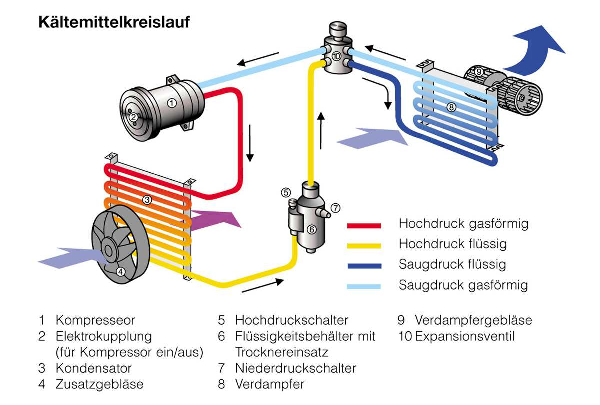
\includegraphics[width=0.7\textwidth]{images/Klima/Klimakreislauf-1.pdf}
\caption{Klimakreislauf}
%\label{fig:}%% anpassen
\end{figure}

\begin{enumerate}
\item
  \textbf{Kompressor} (Gasverdichter, gasförmig, Verdichten, Druck
  steigt) saugt das abgekühlte gasförmige Kältemittel an und verdichtet
  es. Druck und Temperatur steigt (Druckanstieg). Das Kältemittel
  erwärmt sich, wird aber nicht komplett flüssig. Deshalb schieben wir
  es durch den Kondensator.
\item
  \textbf{Kondensator} (Verflüssiger, Kondensieren) hier wird das
  Kältemittel von der Umgebungsluft durchströmt und abgekühlt.
  Aggregatzustand wechsel von gasförmig $\to$ flüssig (Druck ist
  konstant). Kältemittel wird flüssig, wenn es den Kondensator verlässt.
\item
  \textbf{Expansionsventil} (Dosiereinheit, Druckminderer, Drossel,
  Expandieren, flüssig) Kältemittel expandiert durch die Drossel (Druck
  abfall) und lässt bedarfsgerecht eine bestimmte definierte Menge
  Kältemittel durch Strömen.
\item
  \textbf{Verdampfer} (Verdampfen) dadurch wird ein Aggregatzustand
  wechsel von flüssig $\to$ gasförmig (Druck ist konstant)
  gewährleistet. Die durch den Verdampfer strömende Umgebungsluft
  runterkühlen und in den Innenraum einströmen lassen. Dabei entzieht
  das Kältemittel der Umgebungsluft Wärme und kühlt sie ab.
\end{enumerate}

\newpage

\subsection{Kunde bemängelt, Klimaanlage kühlt nicht
richtig}\label{kunde-bemaengelt-klimaanlage-kuehlt-nicht-richtig}

\textbf{Es wurde beispielsweise nur 100 g Kältemittel abgesaugt. Kann
die Klimaanlage wieder befüllt werden?}

Nicht befüllen $\to$ wir machen uns strafbar.

Kältemittel absaugen und mit Stickstoff auf Undichtigkeit prüfen.

\textbf{Verlust an Kältemittel}
$[\%] \, \boxed{= \frac{\text{abgesaugte Menge}}{\text{Füllmenge}} \cdot 100} \quad \text{Beispiel: } \frac{180~g}{640~g} \cdot 100 = 28~\%$

Jährlich ca. $10~\%$ Verlust normal.

\subsection{Was ist der Unterschied zwischen intern und extern geregelte
Klimakompressoren?}\label{was-ist-der-unterschied-zwischen-intern-und-extern-geregelte-klimakompressoren}

\textbf{Intern}, die Stellung der Taumelscheibe und damit die
Fördermenge wird durch ein Regelventil bestimmt. Kann bei Bedarf über
eine Magnetkupplung entkoppelt und damit komplett ausgeschaltet werden.

\emph{Nachteil:} >>kaputt stehen<< eine Klimaanlage nimmt Schaden, wenn
sie nicht regelmäßig eingeschaltet wird (Dichtungen, Schmierung)

\textbf{Extern} keine Magnetkupplung, mit Überlastschutz, Anlage läuft
immer, aber Fördermenge wird runtergeregelt auf ca. $2~\%$

\emph{Nachteil:} Reibung

\subsection{Kältemittel R744 - Problem bei hohen
Außentemperaturen}\label{kaeltemittel-r744-problem-bei-hohen-aussentemperaturen}

Klima funktioniert schlecht bei zu hohen Außentemperaturen
$> 35^\circ\text{C}$. Kältemittel wird nicht genug runtergekühlt.

\subsection{Warum sollte man eine Klimaanlage spülen und welche
Möglichkeiten gibt
es?}\label{warum-sollte-man-eine-klimaanlage-spuelen-und-welche-moeglichkeiten-gibt-es}

Bei Verunreinigungen, Beispiel Kompressor schaden.

\begin{itemize}
\item
  Sieb Einsätze
\item
  Formiergas, Stickstoff, mit Kältemittel (Quelle: Andreas Lamm)
\end{itemize}

\textbf{Offene Anlage} Trockner erneuern oder Anlage verschließen.

\subsection{Desinfizieren einer
Klimaanlage}\label{desinfizieren-einer-klimaanlage}

\begin{itemize}
\item
  Ozongeräte (24h)
\item
  Spray (geringe Wirkung)
\end{itemize}

\subsection{Warum läuft aus der Klimaanlage Wasser bei heißem
Wetter?}\label{warum-laeuft-aus-der-klimaanlage-wasser-bei-heissem-wetter}

\begin{itemize}
\item
  \textbf{Sommer} schwüles Wetter hat eine hohe Luftfeuchtigkeit
\item
  \textbf{Winter} kalte Luft hat eine geringe Luftfeuchtigkeit
\end{itemize}

\subsection{Welche Kältemittelöle gibt es und wo ist der
Unterschied?}\label{welche-kaeltemitteloele-gibt-es-und-wo-ist-der-unterschied}

Herstellerangaben befolgen - Typenschild auf dem Klimakompressor

\begin{itemize}
\item
  \textbf{PAG-Öle} hygroskopisch
\item
  \textbf{POE-Öle} Polyester-Öl, elektrisch isolierendes
  Klimakompressoröl
\end{itemize}

\newpage

\section{Klimaservice}\label{klimaservice}

\textbf{Ruhedruck} (Motor aus)

\begin{itemize}
\item
  Kältemitteldruck abhängig von Umgebungstemperatur (Vgl. Dampftafel /
  Richtwerte \textcite{schmidt:2015:klima} S. 120)
\end{itemize}

\textbf{Betriebsdruck} (Motor an im LL, Klima ON, max. Gebläse, keine
Umluft, Heizung OFF, Temp. LOW, $5 - 10~\text{Min.}$ laufen lassen)

\begin{itemize}
\item
  \textbf{Sollwerte} Quelle: Andreas Lamm \footnote{\url{https://klimacheck.com/}}
\item
  ND $1 - 3~\text{bar}$
\item
  HD $7 - 20~\text{bar}$
\item
  Kühlung

  \begin{itemize}
  \item
    Außentemperatur $20^\circ \text{C} \to 2 - 8^\circ \text{C}$
    \textbf{Ausströmtemperatur}
  \item
    Außentemperatur $30^\circ \text{C} \to \, <15^\circ \text{C}$
    Ausströmtemperatur
  \end{itemize}
\end{itemize}

\subsection{Klimadiagnose}\label{klimadiagnose}

\begin{enumerate}
\item
  Betriebsdruck (Vgl. Sollwerte)

  \begin{itemize}
  \item
    \textbf{Läuft Kondensatorlüfter?}

    \begin{itemize}
    \item
      Wenn Defroster EIN, dann muss Lüfter laufen!
    \end{itemize}
  \end{itemize}
\item
  Ausströmtemperatur (Vgl. Sollwerte)
\item
  Zustand Kältemittel (Schauglas)
\end{enumerate}

\emph{Vgl. Diagnosetabelle}

\begin{table}[!ht]% hier: !ht 
\centering 
	\caption{}% \label{tab:}%% anpassen 
\begin{tabular}{@{}lll@{}}
\hline
\textbf{Hochdruck} & \textbf{Niederdruck} & \textbf{Ursache} \\
\hline
normal, zu hoch & zu niedrig & Expansionsventil, Filter, Kondensator \\
normal, zu niedrig & zu hoch & zu viel Kältemittel, Kompressor \\
normal, zu niedrig & zu niedrig & zu wenig Kältemittel,
Magnetkupplung \\
zu niedrig & zu hoch & zu viel Kältemittel, Kondensator,
Kondensatorlüfter \\
\hline
\end{tabular} 
\end{table}

Anhand der Leitungstemperaturen auf mögliche Defekte im
Kältemittelkreislauf schließen (\textcite{schmidt:2015:klima} S. 115).

Übersicht über fehlerhafte Füllmengen und Komponenten, die sich an den
Druckmanometern widerspiegeln können (\textcite{schmidt:2015:klima} S. 116
-- 117).

\subsection{Magnetkupplung und Kondensatorlüfter
prüfen}\label{magnetkupplung-und-kondensatorluefter-pruefen}

\textbf{Magnetkupplung am Kompressor prüfen}

\begin{enumerate}
\item
  Spannungsversorgung prüfen (Verkabelung, Sicherung, Relais)

  \begin{enumerate}
  \def\labelenumii{\arabic{enumii}.}
  \item
    Magnetkupplung (Spannung am Verbraucher) Soll: $12~V$
  \item
    Masseanschluss (gegen Masse) Soll: $0~V$
  \item
    Relais (gegen Masse) Soll: $12~V$
  \item
    Druckschalter (gegen Masse) Soll: $12~V$
  \end{enumerate}
\item
  Temperatur- und Druckschalter, Steuergerät, Luftspalt
\end{enumerate}

\textbf{Kondensatorlüfter prüfen}

\begin{itemize}
\item
  Sicherung, Relais, Verkabelung, Motor, schwergängig
\end{itemize}

\subsection{Klima-Service-Gerät}\label{klima-service-geraet}

\begin{itemize}
\item
  Vakuumzeit
  $\boxed{60~Min/kg \cdot \text{Kältemittelmenge [kg]}} \quad (1~h~\hat =~ 1~kg)$
\item
  Füllung
\item
  Kompressor-Öl
\end{itemize}

Phasen

\begin{enumerate}
\item
  \textbf{Absaugen} (von Kältemittel und Kompressoröl)
\item
  \textbf{Evakuieren} (Vakuum, Wasser entfernen, Dichtigkeit prüfen)
\item
  \textbf{Aufbereiten} (Kältemittel von Wasser und Öl trennen und
  wiegen)
\item
  \textbf{Auffüllen} (von Kältemittel und Kompressoröl)
\end{enumerate}

\chapter{07-Gemischbildung-Diesel}
%%ju 17-Sep-22 07-Gemischbildung-Diesel.tex
\section{Eigenschaften Dieselmotor}\label{eigenschaften-dieselmotor}

\begin{enumerate}
\item
  Selbstzündung (Kompressionszündung)
\item
  Innere Gemischbildung (Brennraum)
\item
  Qualitative Gemischregulierung (Die eingespritzte Kraftstoffmenge
  reguliert die Leistung des Motors.)
\item
  Heterogenes Gemisch (Das Gemisch aus Luft und Kraftstoff ist im
  Brennraum nicht gleichmäßig verteilt.)
\item
  Hohes Luftverhältnis (Luftüberschuss, d.h. das Verhältnis von Luft zu
  Kraftstoff ist sehr groß.)
\item
  Zündwilliger Kraftstoff (hoch siedend, hohe Cetanzahl)
\end{enumerate}

\section{Warum gibt es einen Klopfsensor beim
Diesel?}\label{warum-gibt-es-einen-klopfsensor-beim-diesel}

Einspritzüberwachung (früher Nadelbewegungssensor): Einspritzbeginn,
Zündbeginn, wie sauber ist die Verbrennung?

\textbf{Was ist ein Klopfsensor?} (am Motorblock verbaut) Piezo-Element:
wenn die seismische Masse in Schwingung gerät, wird durch die Bewegung
eine Spannung erzeugt und im SG verarbeitet. Eine klopfende Verbrennung
wird durch eine ungewöhnlich große Schwingung im Motor erkannt.

\section{Welche Arten von Dieselmotoren gibt
es?}\label{welche-arten-von-dieselmotoren-gibt-es}

\begin{itemize}
\item
  Direkteinspritzung (erste 1988 Audi)
\item
  Indirekte Einspritzung (Vorkammer)

  \begin{itemize}
  \item
    kugelförmig - Vergrößerung der Oberfläche - Wärmeverluste $\to$
    kompensieren durch hohe Drücke und Temperaturen
  \item
    Vorverbrennung $\to$ weiche Verbrennung
  \end{itemize}
\item
  Saugrohreinspritzung
\item
  Turbo aufgeladen
\end{itemize}

\section{Warum haben wir eine höhere Verdichtungsendtemperatur als die
Selbstentzündungstemperatur?}\label{warum-haben-wir-eine-hoehere-verdichtungsendtemperatur-als-die-selbstentzuendungstemperatur}

Das Gemisch muss sich schlagartig und schnell genug entzünden und sauber
genug durchbrennen.

Gay-Lussac - Faktor 2 S. 193 (\textcite{brand:2020:fachkundeKfz}) Erwärmt
man das Gas um $273~K$, so dehnt es sich auf das doppelte aus.
Verhindert man die Ausdehnung beim Verdichten, so verdoppelt sich der
Druck.

\begin{itemize}
\item
  Verdichtungsverhältnis: $14 - 27:1$
\item
  Verdichtungsendtemperatur (Lufttemperatur):
  $600 - 900^\circ\text{C}$
\item
  Verdichtungsenddruck: $30 - 55~\text{bar}$
\item
  Verbrennungshöchstdruck: $200~\text{bar}$
\item
  Druck beim Öffnen des Auslassventils: $4 - 6~\text{bar}$
\item
  Abgastemperatur: $550 - 750^\circ\text{C}$
\end{itemize}

\textbf{vgl. Otto-Saugmotor}

\begin{itemize}
\item
  Verdichtungsverhältnis: $7-12:1$
\item
  Verdichtungsendtemperatur (Lufttemperatur) $400 - 500^\circ\text{C}$
\item
  Verdichtungsenddruck: $18~\text{bar}$
\item
  Verbrennungshöchstdruck: $30 - 60~\text{bar}$
\item
  Druck beim Öffnen des Auslassventils: $3 - 5~\text{bar}$
\item
  Abgastemperatur: $900^\circ\text{C}$
\end{itemize}

Ein \textbf{Arbeitsspiel} läuft in zwei Kurbelwellenumdrehungen ab
$720^\circ\text{KW}$ (Kurbelwinkel). Die \textbf{vier Takte des
Arbeitsspieles} sind Ansaugen, Verdichten, Arbeiten und Ausstoßen.
\textbf{Ein Takt} ist zwischen UT und OT.

\textbf{Ottomotor / Saugrohreinspritzung}

\begin{enumerate}
\item
  Motor / Drosselklappe (fast geschlossen -- offen)
\item
  Ansaugen (geringe -- maximale Menge Kraftstoff-Luftgemisch)
\item
  Füllung (schlecht -- maximal)
\item
  Verdichtungshöchstdruck (gering -- maximal)
\item
  Zündung des Kraftstoff-Luftgemisches, nach der Verbrennung
\item
  Verbrennungshöchstdruck (gering -- maximal)
\item
  wirkt auf die Kolbenfläche und wird auf $\to$ Kolben $\to$ Pleuel
  $\to$ Kurbelwelle übertragen
\item
  Drehmoment an Kurbelwelle (gering -- maximal)
\item
  Drehzahl des Motors (gering -- maximal)
\end{enumerate}

\section{Nageln}\label{nageln}

\textbf{Nageln} harter Motorlauf und zu großer Zündverzug, zum Beispiel
beim Kaltstart des Motors (schlagartige Verbrennung), kann gemindert
werden durch Voreinspritzung.

\textbf{Zu großer Zündverzug tritt ein \ldots{}}

\begin{enumerate}
\item
  kaltem Motor oder kalter Ansaugluft
\item
  schlechter Kompression
\item
  Kraftstoff mit zu niedriger Cetanzahl
\item
  tropfenden Injektoren
\end{enumerate}

\section{Quantitätsregelung und
Qualitätsregelung}\label{quantitaetsregelung-und-qualitaetsregelung}

\textbf{Quantitätsregelung} Ottomotor - Regulierung über die
Gemischmasse, Drosselklappe (Lastzustand) Menge von Luftmasse
(Luftmassenmesser) und Kraftstoffmasse, um das Ziel Lambda = 1 zu
erreichen, wird die Kraftstoffmasse angepasst.

\textbf{Qualitätsregelung} Dieselmotoren - Regulierung über die
Kraftstoffmasse, keine Drosselklappe (systembedingt) nahezu konstante
gleiche Menge Luftmasse, aber die Größe der Kraftstoffmasse kann
geändert werden in Abhängigkeit des Lastwunsches.

\section{Verbrennungsablauf beim
Dieselmotor}\label{verbrennungsablauf-beim-dieselmotor}

\textbf{Verbrennung am Kraftstofftröpfchen} Ausgangslage: Dieseltropfen
wird eingespritzt, Umgebungsluft $600 - 900^\circ\text{C}$,
Kraftstofftröpfchen so gut wie möglich zu verdampfen.

Das Ziel ist ein zündfähiges Gemisch an der Außenlufttemperatur von
selbst zu entzünden, da nur eine sehr geringe Zeit zwischen
Einspritzzeit und kurz vor Ende des Verbrennungsprozesses besteht. Um
die Kraftstofftröpfchen so klein wie möglich zu halten, werden sehr hohe
Drücke und Temperaturen angestrebt.

\textbf{Unvollständige Verbrennung} (durch Sauerstoffmangel)

Wie kann das sein, wir haben doch Sauerstoffüberschuss?

Je größer der Kraftstofftropfen, desto größer ist der Bereich, wo
Luftmangel herrscht.

\textbf{Ursachen für Partikel und Rußbildung} durch unvollständige
Verbrennung

\begin{enumerate}
\item
  Kaltstart- und Warmlaufphase (kalter Motor hat geringere Kompression,
  Kondensationsverluste an Zylinderwand, Wärmeabgabe an Brennraumwände)
\item
  Volllastbetrieb (Kraftstoffüberschuss)
\item
  Sauerstoffmangel (verstopfter Luftfilter, defekter Turbolader,
  undichter Ladeluftkühler)
\item
  Defekte Injektoren (schlechtes Strahlbild, tropfen nach $\to$ mehr
  Kraftstoff)
\item
  Kompressionsverluste (Blow-by, Verdichtungstemperatur wird später
  erreicht)
\end{enumerate}

\section{Was ist EDC? Nenne Vorteile, Ziele und
Merkmale}\label{was-ist-edc-nenne-vorteile-ziele-und-merkmale}

\textbf{EDC} Electronic Diesel Control, Kennfeld (Sollwerte) geregeltes
elektronisches Einspritzsystem

\textbf{Vorteile} bedarfsgerechte Regelung

\textbf{Ziele} Einspritzbeginn und Kraftstoffmenge exakt zu regeln

\textbf{Merkmale} Optimieren von Schadstoffen, Verbrauch, Drehmoment und
Leistung, Laufruhe

\section{Was sind die Hauptsteuergrößen eines jeden
Motors?}\label{was-sind-die-hauptsteuergroessen-eines-jeden-motors}

Last und Drehzahl (Fahrpedalwertsensor, Drehzahlsensor der Kurbelwelle)

\textbf{Korrektursteuergrößen} anpassen der Grundeinspritzzeiten
(abhängig vom Motor)

Einspritzbeginn, $NO_\text{x}-\text{Wert}$, Motortemperatur,
Fahrgeschwindigkeit, AGR-Rate, Ladedruck, Ansauglufttemperatur,
Kraftstofftemperatur, usw.

\section{Einspritzsysteme}\label{einspritzsysteme}

\begin{enumerate}
\item
  \textbf{Reiheneinspritzpumpe}

  \begin{itemize}
  \item
    Einspritzdruck bis etwa 1300 bar
  \item
    Mengenregelung und Förderbeginn (Fliehkraftregler)
  \end{itemize}
\item
  \textbf{Axialkolben-Verteilereinspritzpumpe} (VE)

  \begin{itemize}
  \item
    Einspritzdruck bis etwa 1400 bar
  \item
    Mengenregelung (Verschieben des Regelschiebers) und Förderbeginn
    (hydraulische Spritzversteller), Drehzahl (Fliehkraftregler)
  \end{itemize}
\item
  \textbf{Radialkolben-Verteilereinspritzpumpe} (VP44)

  \begin{itemize}
  \item
    Einspritzdruck bis etwa 1900 bar
  \end{itemize}
\item
  \textbf{Pumpe-Düse-System mit Magnetventil}

  \begin{itemize}
  \item
    Einspritzdruck bis etwa 2200 bar
  \end{itemize}
\item
  \textbf{Pumpe-Düse-System mit Piezoventil}
\item
  \textbf{Pumpe-Leitung-Düse-System} (PLD, Nfz)
\item
  \textbf{Common-Rail}
\end{enumerate}

\subsection{Pumpe-Leitung-Düse-System}\label{pumpe-leitung-duese-system}

Pro Zylinder ein Pumpenelement und eine Einspritzdüse. Einspritzdruck
bis etwa 1800 bar. Eine elektrisch geregelte Voreinspritzung ist
aufgrund der Trägheit des Systems nicht möglich (Länge der
Kraftstoffwege). Um eine Voreinspritzung realisieren zu können, kommen
spezielle Einspritzdüsen zum Einsatz. Die sogenannten
Zweifeder-Düsenhalter (kleine Feder - Voreinspritzung, große Feder -
Haupteinspritzung).

\newpage

\subsection{Pumpe-Düse-System mit
Magnetventil}\label{pumpe-duese-system-mit-magnetventil}

\textbf{Erkläre die Vorgänge - Befüllen, Voreinspritzung,
Haupteinspritzung eines PDE}

\textbf{Befüllen} bei ablaufenden Einspritznocken wird der Pumpenkolben
nach oben gezogen und der Hochdruckraum wird mit Kraftstoff befüllt.
Solange Magnetventil offen ist, fließt der Kraftstoff durch den
Hochdruckraum in den Rücklauf ab. (kühlende Wirkung)

Bei auflaufenden Nocken wird der Pumpenkolben nach unten gedrückt. Das
\emph{Magnetventil} ist geschlossen und verschließt Kraftstoff Vor- und
Rücklaufleitung. Es baut sich ein Hochdruck auf.

\textbf{Voreinspritzung} (Beginn) bei etwa 180 bar ist der Druck größer
als die Düsen-Federkraft. Durch das Einspritzen des Kraftstoffs haben
wir einen kurzen Druckabfall und die Düsennadel schließt (Ende).

Der Ausweichkolben hat seine schräge Druckschulter freigegeben (große
Fläche, große Kraft), wodurch er nach unten gedrückt wird und spannt die
Düsenfeder vor.

\emph{Magnetventil} öffnet und der überschüssige Kraftstoff entweicht in
die Vor- und Rücklaufleitung.

\textbf{Haupteinspritzung} der Druck steigt weiter und drückt bei etwa
300 bar die Düsennadel nach oben (Ende). Durch den Druckabfall schließt
die Düsennadel.

\begin{figure}[!ht]% hier: !ht
\centering
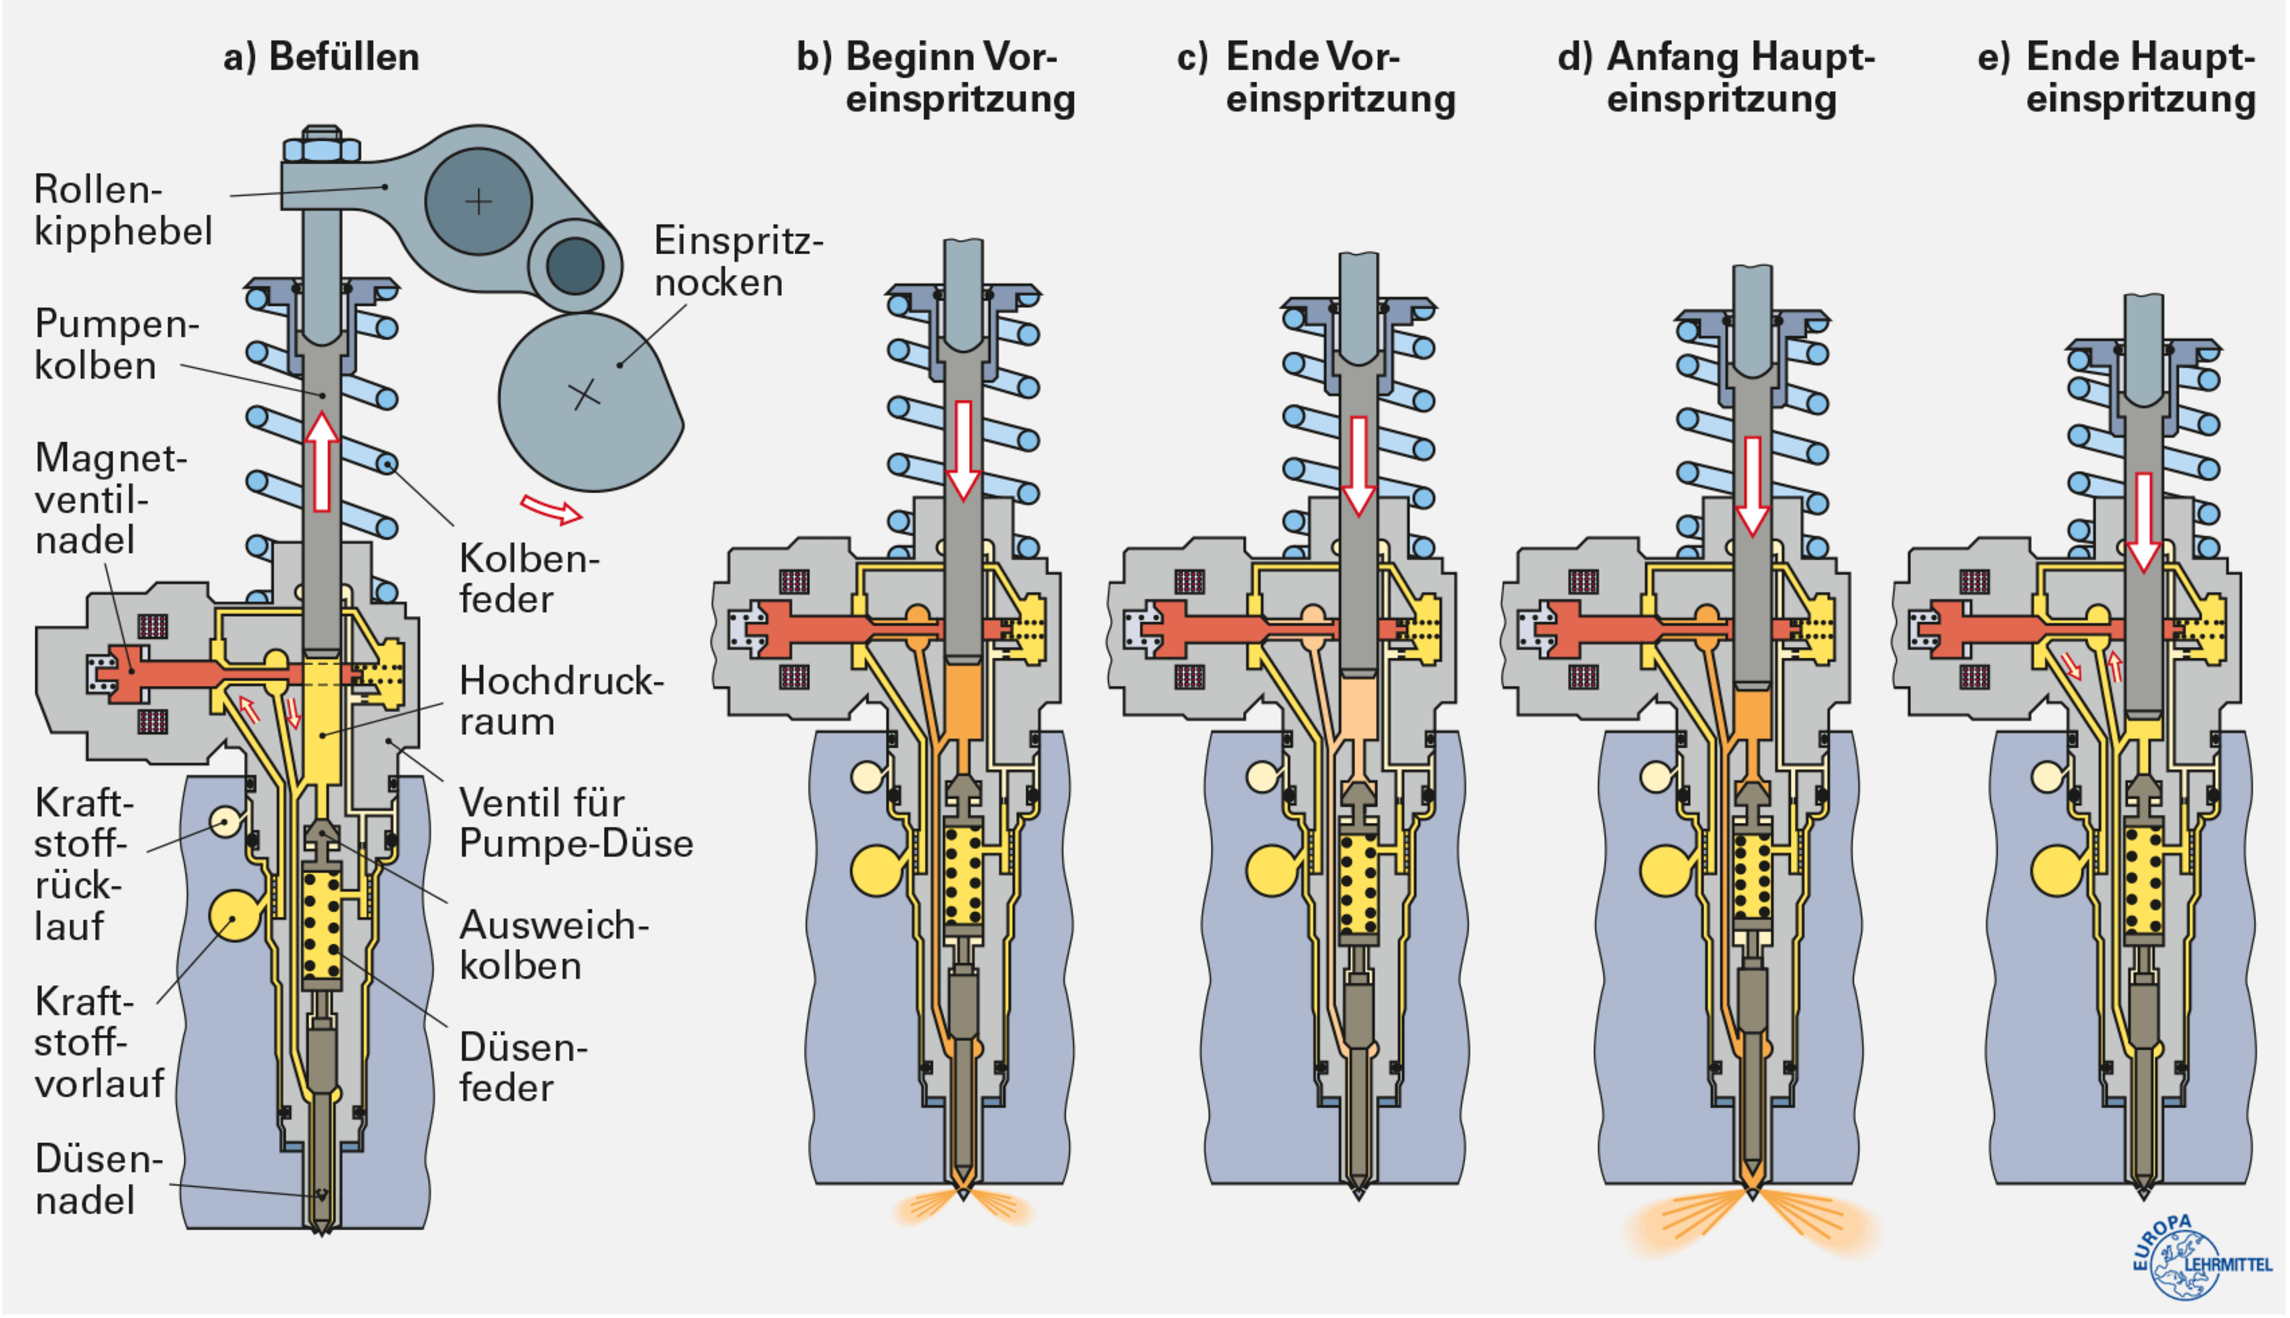
\includegraphics[width=0.7\textwidth]{images/CR/Pumpe-Duese-Elements.png}
\caption{Pumpe-Düse-Element (PDE), Quelle: Europa-Verlag SimKfz}
%\label{fig:}%% anpassen
\end{figure}

\textbf{Nachteile des Pumpe-Düse-Systems mit Magnetventil}

\begin{enumerate}
\item
  Druckerzeugung ist abhängig von Einspritznocken zum Pumpenkolben
\item
  Druck ist nicht konstant, sondern 300 bis 2200 bar
  (Kraftstofftröpfchengröße)
\item
  Hohe Kräfte können auf den Zahnriemen wirken
\item
  Keine Nacheinspritzung (zu Regeneration von DPF)
\item
  Kein mehrmaliges Vorspritzen möglich
\end{enumerate}

\subsection{Pumpe-Düse-System mit
Piezoventil}\label{pumpe-duese-system-mit-piezoventil}

\textbf{Piezoelektrische-Effekt}, übt man auf einen Piezokristall Druck
aus, so erzeugt dieser eine Spannung. (Druck / Krafteinfluss =
Spannungserzeugung)

\emph{Anwendung:} Klopfsensor, Drucksensor (Click-Feuerzeug)

\textbf{Reziproker Piezoelektrischer-Effekt} legt man an einen
Piezokristall eine Spannung an, so verformt er sich. Die Längenänderung
ist proportional zur angelegten Spannung. (Verformung durch
Spannungseinfluss)

\emph{Anwendung:} Injektor

Kfz: Steuerspannung 110-150 V, max. Ausdehnung 0,15 \%

Piezoventil ersetzt Magnetventil (Trägheit - Magnetventil bewegt sich
zeitversetzt, weil der Magnetfeldaufbau gehemmt wird, durch
Gegeninduktion)

\textbf{Piezoventil (Piezoaktor)} besteht aus Piezoaktormodul und
Übersetzermodul (kl. Hebelwerk)

Die Längenausdehnung eines Piezokristalls liegt bei maximal 0,15 \%
(sehr gering). Werden, bis zu 500 Piezokristalle in Reihe geschaltet ist
die Gesamtausdehnung des Piezoaktormodul etwa 0,04 mm. Zum Erreichen der
erforderlichen Ventilöffnung von 0,1 mm wird ein kleines Hebelwerk,
sogenannte Übersetzermodul zwischen Piezoaktormodul und hydraulischen
Ventil geschaltet.

\textbf{Piezoventil geschlossen}, die Verbindung zwischen Hochdruckraum
zur Vor- und Rücklaufleitung ist unterbrochen. Hochdruck kann sich
aufbauen und es wird eingespritzt.

\textbf{Piezoventil offen}, die Verbindung zwischen Hochdruckraum zur
Vor- und Rücklaufleitung ist wieder hergestellt. Hochdruck entweicht und
der Einspritzvorgang ist beendet.

\section{Einspritzventile}\label{einspritzventile}

\begin{itemize}
\item
  Ein- und Zweifeder-Düsenhalter
\item
  Loch- und Zapfendüsen
\end{itemize}

\textbf{Prüfen:} Öffnungsdruck, Strahlbild

\chapter{07-Loesung-Gemischbildung-Diesel}
%%ju 17-Sep-22 07-Loesung-Gemischbildung-Diesel.tex
\textbf{1) Was versteht man unter innerer Gemischbildung beim
Dieselmotor?}

Darunter versteht man, dass das Gemisch im Zylinderraum des Motors
entsteht. Der Dieselkraftstoff also erst dort mit der Ansaugluft in
Berührung kommt.

\textbf{2) Definieren Sie Quantitätsregelung und Qualitätsregelung.}

\begin{enumerate}
\item
  Unter einer \textbf{Quantitätsregelung} versteht man, dass der Motor
  durch eine Anpassung der Gemischmasse zum Beispiel durch eine
  Drosselklappe geregelt wird.
\item
  Bei einer \textbf{Qualitätsregelung} erfolgt die Luftzufuhr nahezu
  Last unabhängig. Lediglich die Kraftstoffmasse wird mit zunehmender
  Last erhöht.
\end{enumerate}

\textbf{3) Bei welcher Temperatur wird Dieselkraftstoff zündfähig und
wann entzündet er sich von selbst?}

\begin{enumerate}
\item
  zündfähig bei etwa $60^\circ\text{C}$
\item
  Selbstzündungstemperatur ca. $220 - 255^\circ\text{C}$
\end{enumerate}

\textbf{4) Erklären Sie ausführlich den Verbrennungsablauf im Brennraum
eines direkt einspritzenden Dieselmotors.}

Gegen Ende des Verdichtungstaktes wird Dieselkraftstoff fein zerstäubt,
in die $600 - 900^\circ\text{C}$ heiße Luft eingespritzt. Diese
verdampft über die Oberfläche der entstandenen Kraftstofftropfen. Je
feiner die Zerstäubung des Kraftstoffes, desto größer ist die Oberfläche
im Verhältnis zum Volumen, was den Vergasungsprozess begünstigt. Die
gasförmigen Kohlenwasserstoffe vermischen sich mit der Ansaugluft und
erhitzen sich, bis sich bei ca. $220^\circ\text{C}$ zur
Selbstentzündung des Kraftstoffes kommt. Je nach System wird dieser
Vorgang Last- und Drehzahlabhängig in mehreren Vorgängen unterteilt, um
den Druckanstieg im Zylinder und damit die Laufkultur des Motors zu
begünstigen.

\textbf{5) Unter welchen motorischen Bedingungen entstehen beim
Dieselmotor unverbrannte Kohlenwasserstoffe?}

\begin{enumerate}
\item
  Kaltstart- und Warmlaufphase (kalter Motor hat geringere Kompression,
  Kondensationsverluste an Zylinderwand, Wärmeabgabe an Brennraumwände)
\item
  Volllastbetrieb (Kraftstoffüberschuss)
\item
  Luftmangel (verstopfter Luftfilter, defekter Turbolader, undichter
  Ladeluftkühler)
\item
  Defekte Injektoren (schlechtes Strahlbild, tropfen nach $\to$ mehr
  Kraftstoff)
\item
  Kompressionsverluste (Verdichtungstemperatur wird später erreicht)
\end{enumerate}

\textbf{6) Warum wird beim Dieselmotor bei Volllast über einen größeren
Zeitraum eingespritzt?}

Da bei Volllast der maximale Einspritzdruck eingestellt wird, geht die
Mengenregelung nur über die Zeit.

\textbf{7) Wie groß ist beim Dieselmotor der Luftüberschuss bei Leerlauf
/ Volllast?}

\begin{itemize}
\item
  Leerlauf $\lambda = 10 \dots 18$
\item
  Volllast $\lambda = 1,15 \dots 2$
\end{itemize}

(Luftzahl / Lambda)

\textbf{8) Definieren Sie Zündverzug. Wie groß ist der Zündverzug?}

Die Zeitspanne von Einspritzbeginn an der Einspritzdüse und dem
Zündbeginn des Kraftstoff-Luft-Gemisches im Brennraum.

betriebswarmer Motor: 1 ms

\textbf{9) Wodurch kann es bei betriebswarmem Motor zum Nageln kommen?}

Durch einen zu großen Zündverzug.

\textbf{Mögliche Ursachen:}

\begin{enumerate}
\item
  zu früher Einspritzbeginn
\item
  Mangelhafte Kompression
\item
  Luftmangel (verstopfter Luftfilter, defekter Turbolader, undichter
  Ladeluftkühler)
\item
  schlechte Kraftstoffqualität (Cetanzahl zu niedrig)
\item
  Nach tropfende Einspritzdüse
\end{enumerate}

\textbf{10) Warum muss beim indirekt einspritzenden Dieselmotor das
Verdichtungsverhältnis 18 - 24:1 betragen, während beim direkt
einspritzenden Dieselmotor ein Verdichtungsverhältnis von 14 bis 18:1
ausreicht?}

Die Oberfläche des Zylinderraumes ist bedingt durch die Vor- oder
Wirbelkammeroberfläche bei indirekt einspritzenden Dieselmotor größer,
wodurch es zu stärkeren Wärmeverlusten kommt. Diese müssen durch eine
stärkere Erwärmung der Luft, also durch ein höheres
Verdichtungsverhältnis, kompensiert werden.

(Eine höhere Kompression kostet aber auch mehr Kompressionsarbeit.)

\chapter{08-Hybrid}
%%ju 31-Dez-22 08-Hybrid.tex
\textbf{Was ist ein Hybridfahrzeug? Hybrid-Vehicle (HV)} ist mit
mindestens zwei unterschiedlichen Energiewandlern und -speichern für den
Antrieb des Fahrzeuges ausgestattet.

Beispiel: Verbrennungsmotor und Kraftstofftank \& E-Motor und
HV-Batterie

\section{Arten von Hybriden}\label{arten-von-hybriden}

\begin{enumerate}
\item
  \textbf{Micro-Hybrid:} Regeneratives Bremsen, Start-Stopp
\item
  \textbf{Mild-Hybrid:} Regeneratives Bremsen, Start-Stopp,
  Drehmomentunterstützung
\item
  \textbf{Full-Hybrid:} Regeneratives Bremsen, Start-Stopp,
  Drehmomentunterstützung, Elektrisches Fahren
\item
  \textbf{Plug-in-Hybrid:} Regeneratives Bremsen, Start-Stopp,
  Drehmomentunterstützung, Elektrisches Fahren, Steckdosenaufladung
\end{enumerate}

\textbf{Boosten} Drehmomentunterstützung (Verbrennungsmotor
unterstützen)

\textbf{Rekuperation} Regeneratives Bremsen (Bremsenergierückgewinnung
$\to$ Batterie Laden)

\section{Antriebskonzepte}\label{antriebskonzepte}

Leistungsverzweigter Hybrid S. 52 (\textcite{schmidt:2021:hybrid}) und
Antriebskonzepte S. 1000 (\textcite{reif:2022:boschkraftfahrtechnisches}).

E-Maschine = \textbf{MG1 / MG2} (E-Motor / Generator), \textbf{V-Motor}
(Verbrennungsmotor), \textbf{Planetengetriebe} (Planetenradsätze und
Lamellenkupplung), Getriebe, Achsantrieb, Inverter (Pulswechselrichter)

\begin{enumerate}
\item
  \textbf{Serieller Hybrid}

  \begin{itemize}
  \item
    Antrieb: durch E-Motor
  \item
    Verbrennungsmotor wird im Drehzahlfenster betrieben (mechanisch
    nicht mit Antriebstrang verbunden)
  \item
    Serieller Energiefluss

    \begin{enumerate}
    \def\labelenumii{\arabic{enumii}.}
    \item
      V-Motor $\to$ Generator $\to$ Inverter $\leftrightarrow$
      HV-Batterie
    \item
      Inverter $\leftrightarrow$ E-Motor $\leftrightarrow$
      Achsantrieb
    \end{enumerate}
  \item
    Nachteil: schlechter Wirkungsgrad ($3\text{x}$ mehr Leistung
    reinstecken!)
  \item
    Beispiel: Range-Extender (Reichweitenverlängerung)
  \end{itemize}
\item
  \textbf{Paralleler Hybrid}

  \begin{itemize}
  \item
    Antrieb: durch E-Motor oder V-Motor (mechanisch mit Antriebstrang
    verbunden) oder beide parallel
  \item
    \emph{eine Kupplung zwischen E-Maschine $\parallel$ Getriebe -
    Achsantrieb}
  \item
    Energiefluss:

    \begin{enumerate}
    \def\labelenumii{\arabic{enumii}.}
    \item
      V-Motor $\to$ Achsantrieb
    \item
      Batterie $\leftrightarrow$ Inverter $\leftrightarrow$ MG
      $\leftrightarrow$ Achsantrieb
    \end{enumerate}
  \item
    \emph{zwei Kupplungen zwischen V-Motor $\parallel$ E-Maschine
    $\parallel$ Getriebe - Achsantrieb}
  \item
    Energiefluss:

    \begin{enumerate}
    \def\labelenumii{\arabic{enumii}.}
    \item
      V-Motor $\to$ Achsantrieb
    \item
      Batterie $\leftrightarrow$ Inverter $\leftrightarrow$ MG
      $\leftrightarrow$ Achsantrieb
    \end{enumerate}
  \end{itemize}
\item
  \textbf{Leistungsverzweigter Hybrid}

  \begin{itemize}
  \item
    Antrieb: durch zwei E-Motoren und V-Motor (mechanisch mit
    Antriebstrang verbunden)
  \item
    Nachteil: aufwändiges Getriebe
  \item
    Leistungsverzweigung (Planetengetriebe)
  \item
    V-Motor (Drehmoment aufteilen)

    \begin{enumerate}
    \def\labelenumii{\arabic{enumii}.}
    \item
      Teil $\to$ MG1 als Generator
    \item
      Teil $\to$ Fahrzeugantrieb
    \end{enumerate}
  \item
    V-Motor + E-Motor $\to$ Fahrzeugantrieb
  \item
    Schub- u. Bremsphase: Generator $\to$ Rekuperation
  \end{itemize}
\end{enumerate}

\chapter{09-Common-Rail-Einspritzung}
%%ju 17-Sep-22 09-Common-Rail-Einspritzung.tex
\begin{figure}[!ht]% hier: !ht
\centering
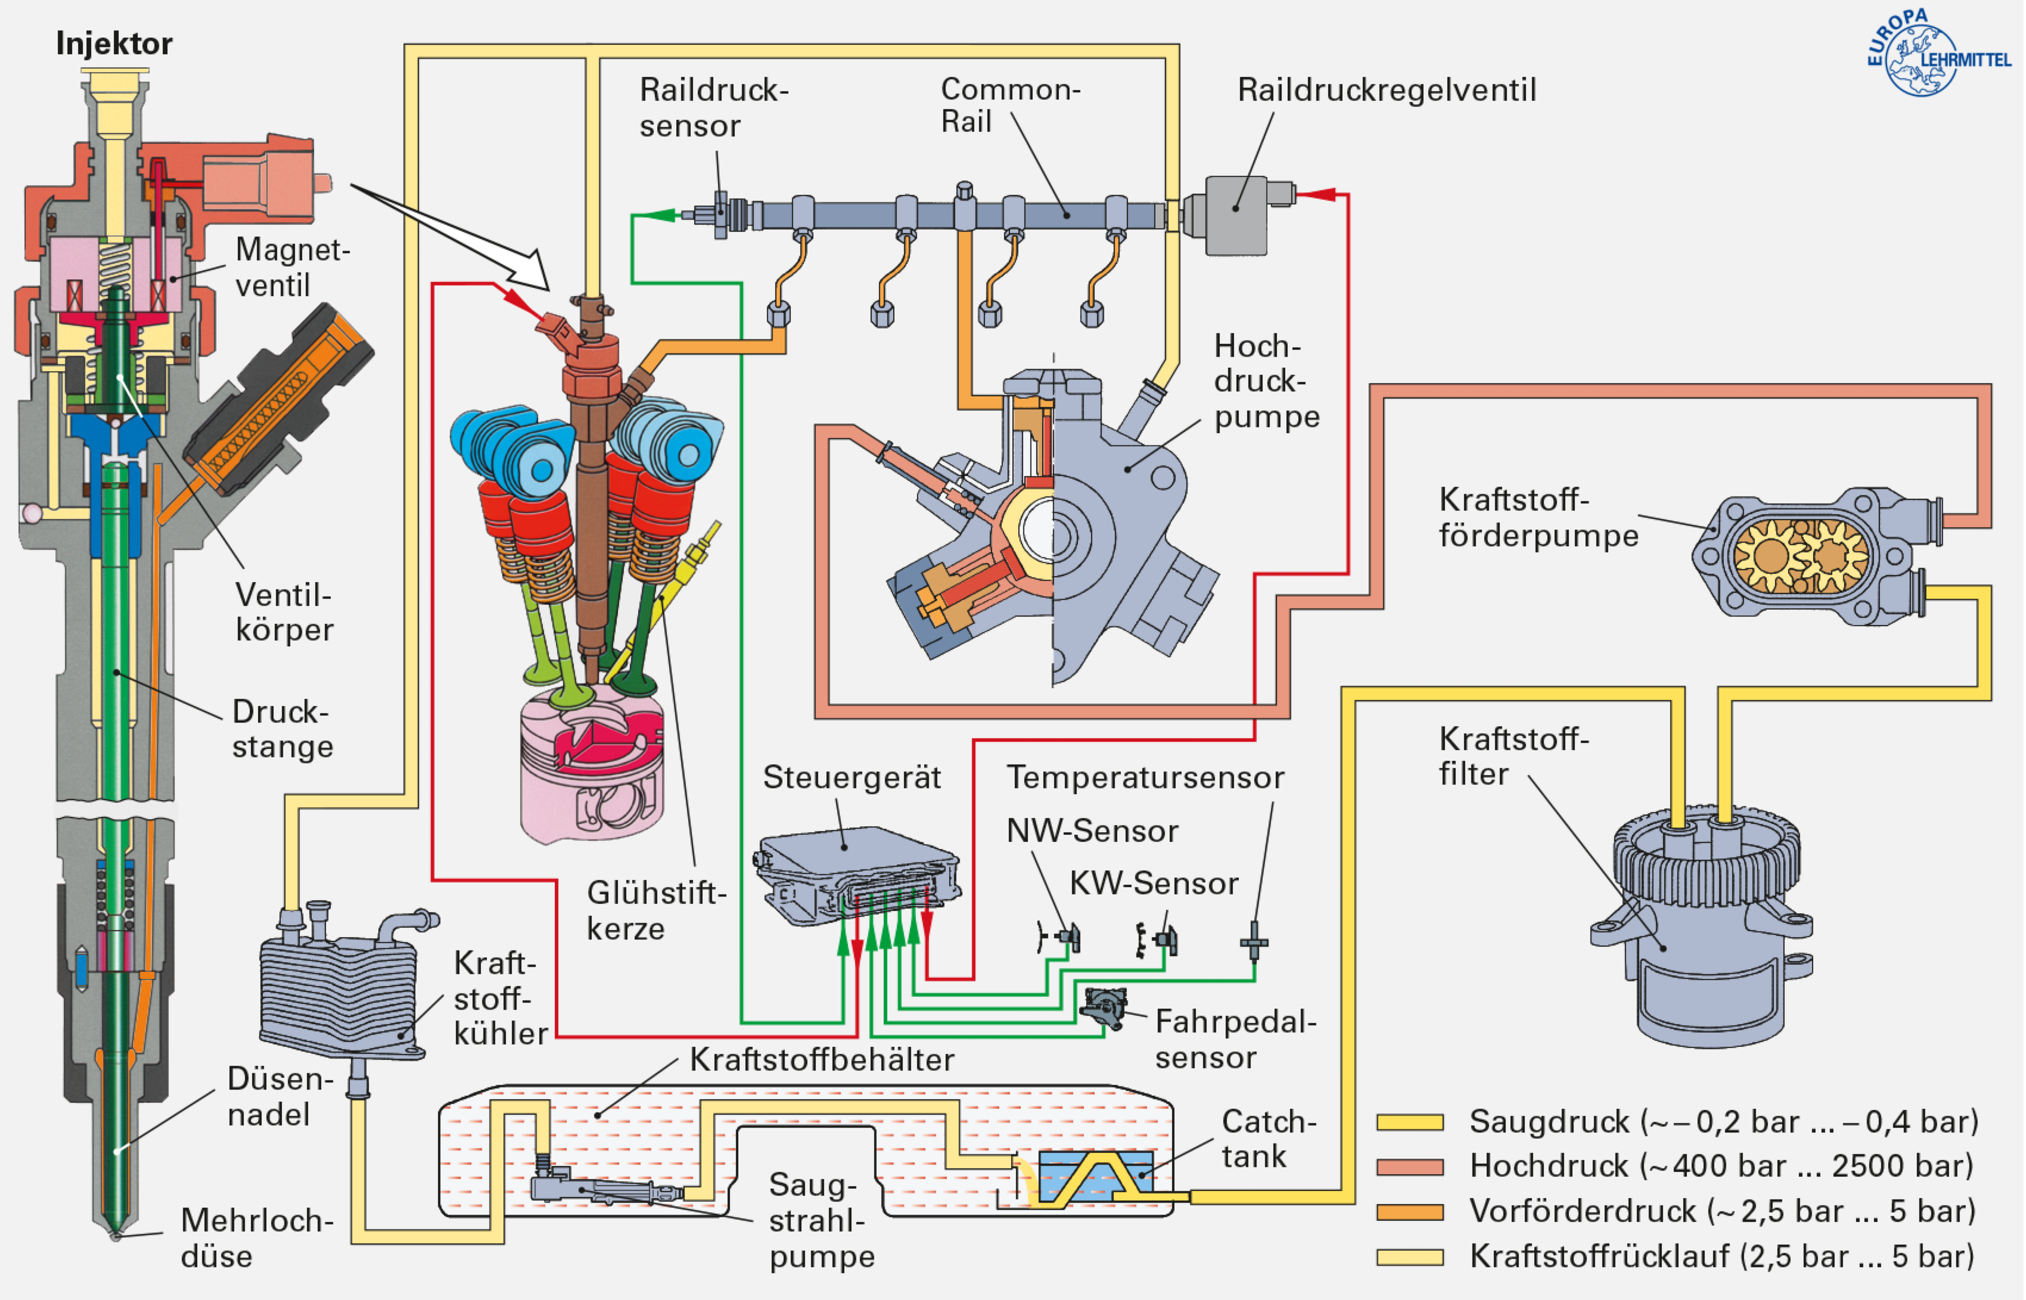
\includegraphics[width=0.7\textwidth]{images/CR/Common-Rail.png}
\caption{Common Rail, Quelle: Europa-Verlag SimKfz}
%\label{fig:}%% anpassen
\end{figure}

\textbf{Bauteile und Aufgaben}

\begin{enumerate}
\item
  \textbf{Elektrische Kraftstoffpumpe} Kraftstoff zu Hochdruckpumpe
  fördern.
\item
  \textbf{Hochdruckpumpe} Kraftstoff unter Hochdruck in das Rail
  fördern.
\item
  \textbf{Rail} Hochdruck speichern und Verteilung des Kraftstoffs auf
  die Injektoren.
\item
  \textbf{Druckregelventil} den erforderlichen Hochdruck an jeden
  Betriebszustand anpassen.
\item
  \textbf{Raildrucksensor} Hochdruck erfassen und als elektrisches
  Signal an das Steuergerät weiterleiten.
\item
  \textbf{Injektor} Kraftstoff dosiert in den Brennraum spritzen
\end{enumerate}

\textbf{Welche Ursachen kommen für den Leistungsverlust infrage?}

\begin{enumerate}
\item
  \textbf{Mechanische Fehler}

  \begin{itemize}
  \item
    Kompressionsverlust durch Verschleiß der Ventile oder des Kolbens
  \item
    Verschleiß der Hochdruckpumpe
  \end{itemize}
\item
  \textbf{Fehler im hydraulischen System}

  \begin{itemize}
  \item
    Undichtigkeit an Injektoren (schließt nicht korrekt, tropft nach,
    Düse ausgewaschen)
  \item
    Undichte Leitungen am Rail
  \end{itemize}
\item
  \textbf{Elektrische Fehler}

  \begin{itemize}
  \item
    Sensoren defekt
  \item
    Aktoren defekt
  \item
    Leitungsunterbrechung
  \item
    Masseschluss
  \end{itemize}
\end{enumerate}

\textbf{Laufruheregelung}, die einzelnen Zylinder bekommen mehr oder
weniger Kraftstoff vom Steuergerät zugeteilt.

\textbf{Was muss beachtet werden beim Einbau eines neuen Injektors?}

\begin{itemize}
\item
  Fertigungstoleranz: muss im Steuergerät einprogrammiert werden
\item
  Zahlen- und Buchstabencodes auf dem Injektor
\item
  Steuergerät korrigiert entsprechend die Grundeinspritzmenge des
  jeweiligen Injektors.
\end{itemize}

\textbf{Erkläre den Spannungs- bzw. Stromverlauf eines intakten
Injektors}

\begin{itemize}
\item
  Injektorspannung beträgt in der Anzugsphase ca. 80 V. Der Anzugstrom
  liegt dadurch bei ca. 20 A. Danach wird der Strom auf ca. 12 A
  begrenzt (Haltestrom), bei einer Spannung von 12 V bis 14 V.
\end{itemize}

\textbf{Wie entsteht die Injektorsspannung von 80 bis 100 V?}

\begin{itemize}
\item
  Beim Ausschalten der Magnetventile wird die entstehende
  Induktionsspannung genutzt, um im Steuergerät einen Kondensator
  aufzuladen.
\end{itemize}

\newpage

\textbf{Welche Druckregelungsarten gibt es?}

\begin{enumerate}
\item
  \textbf{Einsteller-Regelung}

  \begin{itemize}
  \item
    \textbf{Druckregelung hochdruckseitig} (Druckregelung)

    \begin{itemize}
    \item
      Hochdruckpumpe fördert die maximale Fördermenge unabhängig von
      Bedarf an Kraftstoff
    \item
      Raildruck wird über ein Druckregelventil geregelt, nicht
      benötigter Kraftstoff fließt zurück in den Tank
    \item
      \textbf{Nachteil:} Hochdruckpumpe ist konstant maximal belastet,
      dadurch

      \begin{itemize}
      \item
        geringere Nutzleistung
      \item
        erhöhter Kraftstoffverbrauch, Schadstoffausstoß, Verschleiß
      \item
        unnötige Erwärmung des Kraftstoffs
      \end{itemize}
    \end{itemize}
  \item
    \textbf{Druckregelung niederdruckseitig} (Mengenregelung)

    \begin{itemize}
    \item
      Raildruck wird über eine Zumesseinheit an der Hochdruckpumpe
      niederdruckseitig geregelt
    \item
      Bedarfsregelung es gelangt nur so viel Kraftstoff zu
      Hochdruckpumpe wie benötigt wird für die Einspritzung
    \item
      Zumesseinheit regelt die Zuflussmenge zur Hochdruckpumpe

      \begin{itemize}
      \item
        Mengenregelventil unbestromt: voll offen für maximale
        Fördermenge
      \item
        Mengenregelventil bestromt: verringert den Öffnungsquerschnitt
        für minimale Fördermenge\\
      \end{itemize}
    \item
      Druckbegrenzungsventil verhindert zu hohen Raildruck bei Ausfall
      der Zumesseinheit
    \item
      \textbf{Nachteil:}

      \begin{itemize}
      \item
        hohe Trägheit
      \item
        Drucksteigerung erfordert zunächst eine Erhöhung des
        Niederdrucks, dadurch erhöhte Förderleistung der Hochdruckpumpe
      \end{itemize}
    \end{itemize}
  \end{itemize}
\item
  \textbf{Zweisteller-Regelung} (\textbf{Druckregelung nieder- und
  hochdruckseitig})

  \begin{itemize}
  \item
    \textbf{Vorteil}

    \begin{itemize}
    \item
      geringe Leistungsaufnahme der Hochdruckpumpe bei konstant hohen
      Drücken
    \item
      hohe Agilität bei geringen Drücken
    \end{itemize}
  \item
    \textbf{Motorstart und Warmlaufphase} hochdruckseitig geregelt

    \begin{itemize}
    \item
      Kraftstoff soll sich erwärmen und damit fließ- und zündfähiger zu
      machen
    \end{itemize}
  \item
    \textbf{betriebswarmer Motor: Leerlauf / Teillast}
    Zweisteller-Betrieb

    \begin{itemize}
    \item
      große Sprünge des Raildrucks sind wahrscheinlich (Motor im
      Leerlauf / Teillast $\to$ Lastwunsch des Fahrers: Volllast)
    \end{itemize}
  \item
    \textbf{hohen Motorlast} niederdruckseitig geregelt

    \begin{itemize}
    \item
      große Steigerungen des Raildrucks nicht möglich und deshalb ist
      die Trägheit vernachlässigbar
    \end{itemize}
  \end{itemize}
\end{enumerate}

\textbf{Druckregelventil} Druckerfassung durch Membransensor am Rail
(Raildrucksensor)

Ansteuerung: PWM-Signal (Raildruck wird größer, wenn Tastverhältnis
größer wird), wenn Magnetventil bestromt: dadurch wird die Schließkraft
der Ventilnadel erhöht oder gesenkt. Dementsprechend wird der Raildruck
erhöht oder gesenkt.

\begin{enumerate}
\item
  \textbf{unbestromt / stromlos} Raildruck etwa $100~\text{bar}$

  \begin{itemize}
  \item
    Motor abstellen, Ventilfeder hält Druckregelventil geschlossen,
    verhindert ein Leerlaufen des Rails
  \end{itemize}
\item
  Magnetventil bestromt, Lastzustände:

  \begin{itemize}
  \item
    \textbf{Motorstart} Raildruck $> 250~\text{bar}$

    \begin{itemize}
    \item
      Wie hoch ist der Druck im Rail bei Motorstart?
    \end{itemize}
  \item
    \textbf{Leerlauf} Raildruck etwa $400~\text{bar}$
  \item
    \textbf{Vollast} Raildruck etwa $2000~\text{bar}$
  \end{itemize}
\end{enumerate}

\textbf{Warum lässt sich ein Fahrzeug mit defektem Druckregelventil
nicht mehr starten?}

Durch die im Druckregelventil verbaute Feder verbleibt im Rail ein
Restdruck von ca. 100 bar. Da für einen sicheren Motorstart der Druck im
Rail mind. 250 bar betragen muss, ist ein Motorstart nicht möglich.

\newpage

\subsubsection{Injektoren}\label{injektoren}

Injektoren vs.~Einspritzdüsen: haben keinen festen Öffnungsdruck,
sondern öffnen und schließen unter dem jeweiligen variablen
Einspritzdruck.

Kraft = Druck x Fläche

\textbf{Wie werden Piezoinjektoren angesteuert?}

SG $\to$ Spannung anlegen $\to$ Längenänderung, bleibt in Position
bis Kurzschluss $\to$ abschließende Spannung.

\textbf{Erklären Sie die Funktionsweise eines Magnetspuleninjektors im
geschlossenen und geöffneten Zustand.}

\begin{figure}[!ht]% hier: !ht
\centering
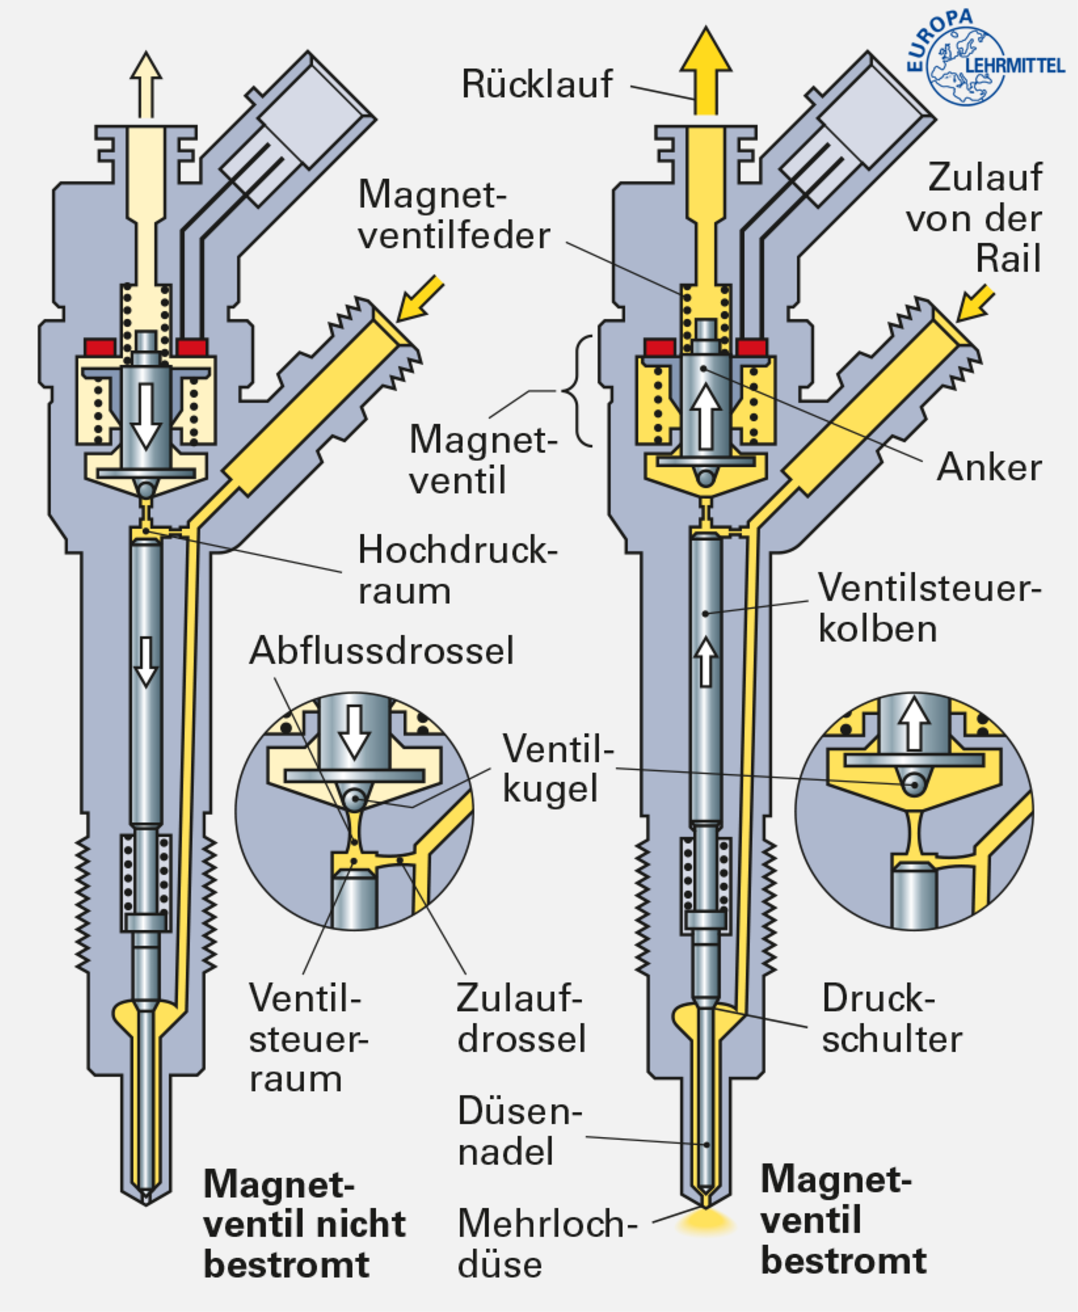
\includegraphics[width=0.4\textwidth]{images/CR/Wirkungsweise-Magnetventilinjektors.png}
\caption{Injektor mit Magnetventil, Quelle: Europa-Verlag SimKfz}
%\label{fig:}%% anpassen
\end{figure}

\begin{itemize}
\item
  \textbf{Magnetventil unbestromt - geschlossenen Zustand} dann wirkt im
  Ventilsteuerraum auf der Stirnfläche des Ventilsteuerkolbens und auf
  der Druckschulter der Düsennadel gleicher Kraftstoffkochdruck.
  Einspritzventil ist geschlossen.
\item
  \textbf{Magnetventil bestromt - geöffneten Zustand,} dann wird der
  Rücklauf geöffnet. Über die Ablaufdrossel entweicht mehr Kraftstoff,
  als über die Zulaufdrossel abfließen kann. Es kommt zum Druckabfall im
  Ventilsteuerraum. Der Druck auf die Druckschulter der Düsennadel kann
  die Düse öffnen. Düsennadel öffnet die Düse.
\end{itemize}

\textbf{Erklären Sie die Funktionsweise eines Injektors mit Piezoventil}

Piezoinjektoren erlauben hohe Schaltgeschwindigkeiten und damit viele
Teileinspritzungen.

\begin{itemize}
\item
  Piezo-Aktormodul wird bestromt und dehnt sich aus.
\item
  Über den hydraulischen Koppler findet eine Hubvergrößerung statt.
\item
  Öffnet das Servoventil und damit den Rücklauf.
\item
  Über die Ablaufdrossel fließt Kraftstoff aus dem Ventilsteuerraum ab.
\item
  Über die Zulaufdrossel kann weniger Kraftstoff in den Ventilsteuerraum
  zufließen. Es kommt zum Druckabfall.
\item
  Der Druck auf die Druckschulter der Düsennadel öffnet die Düsennadel
  des Injektors. Einspritzbeginn.
\end{itemize}

\chapter{Gemischbildung-Ottomotor}
%%ju 26-Dez-22 Gemischbildung-Ottomotor.tex
\section{Gemischbildungssysteme}\label{gemischbildungssysteme}

sollen für jeden Betriebszustand des Motors ein Kraftstoff-Luft-Gemisch
herstellen, das in der \emph{Menge ausreichend} ist und im Motor
möglichst \emph{vollständig verbrannt} wird.

\section{Betriebszustände}\label{betriebszustaende}

\begin{itemize}
\item
  \textbf{Kaltstart}

  \begin{itemize}
  \item
    Kraftstoff kondensiert an kalten Saugrohr- und Zylinderwänden
  \item
    $\to$ sehr fettes Gemisch (bis $\lambda = 0,3$) nötig
  \end{itemize}
\item
  \textbf{Warmlauf}

  \begin{itemize}
  \item
    Kondensationsverluste verringert sich
  \item
    $\to$ Kraftstoffmenge wird temperaturabhängig verringert
  \end{itemize}
\item
  \textbf{Leerlauf}
\item
  \textbf{Übergang, Beschleunigung}

  \begin{itemize}
  \item
    beim Öffnen der Drosselklappe magert das Gemisch kurzzeitig ab
  \item
    $\to$ kurzzeitig mehr Kraftstoff einspritzen
  \end{itemize}
\item
  \textbf{Teillast}
\item
  \textbf{Volllast}

  \begin{itemize}
  \item
    maximale Motorleistung bei voll geöffneter Drosselklappe
  \item
    $\to$ Anreicherung des Gemisches auf $\lambda = 0,85 \dots 0,95$
  \end{itemize}
\item
  \textbf{Schubabschaltung}

  \begin{itemize}
  \item
    Drosselklappe geschlossen bei hoher Drehzahl (Bergab fahren oder Fuß
    vom Gas bei hoher Geschwindigkeit)
  \item
    $\to$ keine Einspritzung von Benzin bis Drosselklappe wieder
    geöffnet
  \end{itemize}
\end{itemize}

\section{Mischungsverhältnis}\label{mischungsverhaeltnis}

beschreibt die \emph{Zusammensetzung des Kraftstoff-Luft-Gemisches}. Man
unterscheidet ein theoretisches und ein praktisches Mischungsverhältnis.

\begin{enumerate}
\item
  \textbf{Theoretisches Mischungsverhältnis} (stöchiometrisches
  Verhältnis):

  \begin{itemize}
  \item
    zur \emph{vollständigen Verbrennung} von $1~kg$ Super werden
    $14,7~Kg$ Luft benötigt
  \end{itemize}
\item
  \textbf{Praktisches Mischungsverhältnis}

  \begin{itemize}
  \item
    weicht je nach Betriebszustand vom theoretischen Verhältnis ab
  \item
    \emph{Fettes Gemisch} (Luftmangel): z. B. $1:13$
  \item
    \emph{Mageres Gemisch} (Luftüberschuss): z. B. $1:16$
  \end{itemize}
\end{enumerate}

\section{Luftverhältnis}\label{luftverhaeltnis}

$\lambda$ ist das Verhältnis zwischen der tatsächlich der Verbrennung
zugeführten Luftmasse und der zur vollständigen Verbrennung theoretisch
erforderlichen Luftmasse

\begin{itemize}
\item
  Luftverhältnis
  $\lambda = \frac{\text{zugeführte Luftmasse in [kg]}} {\text{theoretische Luftmasse in [kg]}}$
\item
  Beim theoretischen Mischungsverhältnis $1:14,7$ ist $\lambda = 1$
\item
  $\lambda = \frac{16~kg}{14,7~kg} > 1$ (mager)
\end{itemize}

\textbf{Mischungsverhältnisse für Super}

\begin{figure}[!ht]% hier: !ht
\centering
\includegraphics[width=0.6\textwidth]{images/skizze/Mischungs-Luftverhaeltnis.pdf}
\caption{Mischungsverhältnis}
%\label{fig:}%% anpassen
\end{figure}

\section{Gemischzusammensetzung}\label{gemischzusammensetzung}

\begin{enumerate}
\item
  \textbf{Homogenes Gemisch}

  \begin{itemize}
  \item
    im gesamten Brennraum ist die Gemischzusammensetzung gleich
  \item
    Einspritzung im Ansaugtakt
  \item
    braucht Zeit für eine gleichmäßige Durchmischung des
    Kraftstoff-Luft-Gemisches
  \end{itemize}
\item
  \textbf{Heterogenes Gemisch}

  \begin{itemize}
  \item
    im Brennraum gibt es Bereiche unterschiedlicher
    Gemischzusammensetzung (\textbf{Schichtladung})

    \begin{itemize}
    \item
      Fettes Gemisch in der Nähe der Zündkerze ($\lambda = 1$)
    \item
      Mageres Gemisch im äußeren Bereich ($\lambda > 1,3$)
    \item
      späte Einspritzung während des Verdichtungstaktes
    \end{itemize}
  \item
    Saugrohrklappe geschlossen
  \item
    man kann sehr mager fahren, um Sprit zu sparen
  \end{itemize}
\end{enumerate}

\textbf{Ort der Gemischbildung}

\begin{enumerate}
\item
  \textbf{Äußere Gemischbildung} Kraftstoff wird in das Saugrohr
  eingespritzt

  \begin{itemize}
  \item
    Homogenes Gemisch
  \end{itemize}
\item
  \textbf{Innere Gemischbildung} Kraftstoff wird direkt in den Brennraum
  eingespritzt

  \begin{itemize}
  \item
    Heterogenes Gemisch

    \begin{itemize}
    \item
      späte Einspritzung während des Verdichtungstaktes kurz vor Zündung
    \item
      Kraftstoff und Luft kann sich nicht gleichmäßig vermischen
    \end{itemize}
  \item
    Homogenes Gemisch

    \begin{itemize}
    \item
      Einspritzung zu Beginn des Ansaugtaktes
    \end{itemize}
  \end{itemize}
\item
  \textbf{Kombi aus äußere und innere Gemischbildung}
\end{enumerate}

\section{Leistungsregelung}\label{leistungsregelung}

\begin{enumerate}
\item
  \textbf{Quantitätsregelung} Motoren mit äußerer Gemischbildung und
  homogenem Gemisch

  \begin{itemize}
  \item
    Je nach Lastzustand ändert sich die Drosselklappe und damit die
    angesaugte Luftmenge.
  \item
    Die Zusammensetzung des Gemisches muss dabei nahezu gleich bleiben
    ($\lambda = 1$)
  \end{itemize}
\item
  \textbf{Qualitätsregelung} Motoren mit innerer Gemischbildung und
  heterogenem Gemisch

  \begin{itemize}
  \item
    Bei geöffneter Drosselklappe wird verschieden viel Kraftstoff
    eingespritzt. Die angesaugte Luftmenge bleibt dabei nahezu gleich
  \item
    Die Zusammensetzung des Gemisches im Brennraum ändert sich somit je
    nach Lastzustand.
  \end{itemize}
\end{enumerate}

\section{Arten der
Benzineinspritzung}\label{arten-der-benzineinspritzung}

\textbf{Vergaser}

Luft wird angesaugt vom Motor, vor der Drosselklappe gibt es eine
Verengung, durch die Verengung erhöht sich die Strömungsgeschwindigkeit
der angesaugten Luft (Venturi-Rohr). Der Kraftstoff im Vergaser gelangt
über eine Düse in Tropfenform in das Ansaugluftgemisch. Durch die hohe
Strömungsgeschwindigkeit der angesaugten Luft wird der Kraftstoff
mitgerissen.

Vorzerstäubung, Feinzerstäubung $\to$ Kraftstoff-Luft-Gemisch

Die Luftdurchflussmenge wird über Luftdruck (Luftdichte) und Temperatur
gemessen. Daraus wird die Düsengröße berechnet und damit die
Kraftstoffmenge.

\textbf{Indirekte Einspritzung}

\emph{Einzelpunkteinspritzung}

\begin{itemize}
\item
  vor der Drosselklappe befindet sich ein Einspritzventil
\item
  die angesaugte Luft wird mit Kraftstoff versetzt, sodass ich hier ein
  Gemisch gebildet habe
\item
  Gemischzusammensetzung war nicht so genau, durch unterschiedliche
  Ansaugwege
\end{itemize}

\begin{table}[!ht]% hier: !ht 
\centering 
	\caption{}% \label{tab:}%% anpassen 
\begin{tabular}{@{}ll@{}}
\hline
\textbf{\#} & \textbf{Beschreibung} \\
\hline
Art der Einspritzung & \textbf{SPI = Single Point Injection} \\
Ort der Einspritzung & Indirekt - vor der Drosselklappe \\
Gemischzusammensetzung & homogen \\
\hline
\end{tabular} 
\end{table}

\emph{Mehrpunkteinspritzung}

\begin{itemize}
\item
  die angesaugte Luft strömt durch die Drosselklappe in das
  Verteilerrohr
\item
  Kraftstoffverteilerrohr mit einzelne Einspitzventilen, die direkt in
  das Saugrohr einspritzen
\item
  Gemischzusammensetzung ist gleich (gleiche Ansaugwege)
\end{itemize}

\begin{table}[!ht]% hier: !ht 
\centering 
	\caption{}% \label{tab:}%% anpassen 
\begin{tabular}{@{}ll@{}}
\hline
\textbf{\#} & \textbf{Beschreibung} \\
\hline
Art der Einspritzung & \textbf{MPI = Multi Point Injection} \\
Ort der Einspritzung & Indirekt - vor das Einlassventil \\
Gemischzusammensetzung & homogen \\
\hline
\end{tabular} 
\end{table}

\textbf{Direkte Einspritzung}

\begin{table}[!ht]% hier: !ht 
\centering 
	\caption{}% \label{tab:}%% anpassen 
\begin{tabular}{@{}ll@{}}
\hline
\textbf{\#} & \textbf{Beschreibung} \\
\hline
Art der Einspritzung & \textbf{MPI = Multi Point Injection} \\
Ort der Einspritzung & Direkt - in den Zylinder \\
Gemischzusammensetzung & homogen oder heterogen \\
\hline
\end{tabular} 
\end{table}

\section{Öffnung der
Einspritzventile}\label{oeffnung-der-einspritzventile}

\begin{itemize}
\item
  Simultane Einspritzung
\item
  Sequenzielle Einspritzung
\item
  Zylinderselektive Einspritzung
\end{itemize}

\section{Zündanlage}\label{zuendanlage}

\textbf{Zündanlage mit Unterbrecherkontakt}

Bat. 12 V $\to$ Zündspannung 40.000 V

Batterie - 30 - Zündschalter - 15 - Zündspule

\begin{itemize}
\item
  1 - Unterbrecherkontakt - Masse wird geschaltet durch Nocken

  \begin{itemize}
  \item
    geschlossen - in Primärspule baut sich Magnetfeld auf
  \item
    offen - Magnetfeld bricht zusammen, es wird eine Spannung in der
    Sekundärspule indiziert - Spannung geht weiter an den Zündverteiler
  \end{itemize}
\item
  4 - Zündverteiler - Zündkerze - Zündfunken - Masse
\end{itemize}

\textbf{Zündanlage mit Einzelfunkzündspule}

\begin{itemize}
\item
  Eingabe - Wann soll gezündet werden?

  \begin{itemize}
  \item
    Positionsgeber an Nockenwelle und Fahrpedal
  \end{itemize}
\item
  Verarbeitung erfolgt im Steuergerät

  \begin{itemize}
  \item
    Kennfeld - abhängig von Drehzahl und Last wird ein Zündwinkel
    berechnet
  \end{itemize}
\item
  Ausgabe an Zündspule
\end{itemize}

\section{Sensoren und Aktoren}\label{sensoren-und-aktoren}

\begin{table}[!ht]% hier: !ht 
\centering 
	\caption{}% \label{tab:}%% anpassen 
\begin{tabular}{@{}lll@{}}
\hline
\textbf{\#} & \textbf{Sensoren} & \textbf{Aktoren} \\
\hline
\textbf{Zentraleinspritzung} & Drehzahlgeber &
Drosselklappenansteller \\
& Motortemperaturfühler & Regenerierventil \\
& Lufttemperaturfühler & Einspritzventil \\
& Drosselklappenpotentiometer & \\
& Lambdasonde & \\
& OT-Geber & \\
\textbf{MED - Motronic} & Luftmassenmesser & Kraftstoffpumpe \\
& Saugrohrdrucksensor & E-Gas Stellmotor \\
& Differenzdrucksensor & Lambdasondenheizung \\
& Fahrpedalsensor & NOx-Sensorheizung \\
& NOx-Sensor & Tankentlüftungsventil \\
& Abgastemperatursensor & Abgasrückführventil \\
& Saugrohrklappenpotentiometer & Kraftstoffdruckregelventil \\
& & Saugrohrklappenventil \\
\hline
\end{tabular} 
\end{table}

\chapter{Kfz-Links}
%%ju 13-Aug-22 Kfz-Links.tex
\textbf{Mathe}

\url{https://mathematrick.de/}

\url{https://www.youtube.com/channel/UCMZgTsrg4GbC7meNeOL86fg}

\url{https://www.youtube.com/channel/UCQZ9qA2fMEXn6kysdywXCdw}

\textbf{Kraftfahrzeugtechnik pur}

\url{https://www.youtube.com/user/kfz4metube/videos}

\textbf{Rebecca Elizabeth}

\url{https://youtube.com/c/RebeccaElizabeth}

\textbf{ccd Car-Diagnostics}

\url{https://www.youtube.com/c/ccdCarDiagnostics}

\textbf{Reynald Hirschi}

\url{https://youtube.com/c/ReynaldHirschi}

\textbf{Fahrzeugakademie}

\url{https://youtube.com/c/FahrzeugakademieDe1}

\textbf{Michael von Werder}

\url{https://www.youtube.com/channel/UCCd9ydGN4dguE_b83b_HrrQ}

\textbf{Motoren Zimmer}

\url{https://motorenzimmer.de}

\url{https://www.youtube.com/channel/UCWAEPOo1hVr_hnSoGvkvJJg}

\textbf{Bloch erklärt}

\url{https://www.youtube.com/channel/UCLINPbYQ9sy6qc-TqtBeVnw}

\textbf{Attractor}

\url{https://www.youtube.com/channel/UCL5DBQu4rk1IoK_shRFXc4w}

\textbf{Die Autodoktoren - offizieller Kanal}

\url{https://www.youtube.com/channel/UCcnmNzv0yEEYPM6Oa86unhQ}

\textbf{Horst Weinkauf}

\url{https://www.horst-weinkauf.de/index.php/downloads}

\textbf{E-Learning Kraftfahrzeugtechnik}

\url{https://www.youtube.com/c/ELearningKraftfahrzeugtechnik}

\chapter{Motoroel}
%%ju 17-Sep-22 Motoroel.tex
\textbf{Aufgabe} Schmieren, Kühlen und vor Korrosion schützen, Reinigen,
Abdichten, Geräusche dämpfen

\textbf{Zusammensetzung}

\begin{enumerate}
\item
  Grundöl $80~\%$

  \begin{itemize}
  \item
    Mineralöl: \emph{Erdöl - Destillieren - schwersiedende Bestandteile
    - Raffinieren (reinigen/veredeln)} z. B. 15W-40, Hochtemperatur
    stabil bis: 130 °C
  \item
    Synthetisches Öl: \emph{Erdöl - Destillieren - Rohbenzin - Cracken}
    z. B. 5W-30, Hochtemperatur stabil bis: 180 °C
  \end{itemize}
\item
  Additive (Eigenschaften verbessern) $20~\%$
\end{enumerate}

\textbf{Viskosität}

\begin{itemize}
\item
  Grad der Zähflüssigkeit (Fließfähigkeit bei niedrigen und hohen
  Temperaturen)
\item
  niedrige Viskosität: dünnflüssig, hohe Viskosität: zähflüssig
\item
  SAE-Viskositätklasse, Mehrbereichsöl, z. B. 5W-30 (Tieftemperatur,
  Winter, Hochtemperatur)
\end{itemize}

\textbf{Hochtemperatur Querstabilität} Schmierfilm nicht abreißen
(Temperatur, Drehzahl abhängig)

\textbf{API - Leistungsklassen (Amerika)}

\textbf{ACEA - Spezifikation (Europa)}

Mindestanforderung an die Qualität von Motorölen

\textbf{Automobilhersteller Spezifikation}

\textbf{Anteil gering} Schwefel, Asche, Phosphor (Abgasnachbehandlung)

\textbf{Ölstand} >>Bei betriebswarmen Motor messen.<<

\begin{enumerate}
\item
  zu wenig
\item
  zu viel (Nachteil)

  \begin{itemize}
  \item
    Öl verbrennen > Motor durchgehen
  \item
    Öl aufschäumen > keine Schmierwirkung
  \end{itemize}
\end{enumerate}

>>Kurzstrecke<< (Wasser, Kraftstoff > Öl)

\begin{itemize}
\item
  Motor kalt: Ölstand hoch
\item
  Motor warm: niedrig
\end{itemize}

\textbf{Haltbarkeit}

\begin{itemize}
\item
  \emph{Altes Öl} ca. drei Jahre haltbar (wenn geöffnet)
\item
  \emph{Neues Öl} ca. fünf Jahre haltbar (original verschlossen)
\end{itemize}

\textbf{Hersteller}

Wolf Öl \footnote{\url{https://www.wolflubes.com/de_de/products/default.aspx}}
5W-30 C1 Produktcode: 65605

Castrol EDGE 5W-30 LL Motorenöl

\chapter{Pruefungstrainer-Kfz-Technik}
%%ju 26-Dez-22 Pruefungstrainer-Kfz-Technik.tex
\section{Kraftfahrzeug, Wartung,
Instandhaltung}\label{kraftfahrzeug-wartung-instandhaltung}

\subsection{Technisches System
Kraftfahrzeug}\label{technisches-system-kraftfahrzeug}

\begin{enumerate}
\item
  Energiefluss\\
\item
  Technik: Energie\\
\item
  Öffnungskraft\\
\item
  Resultierende Kraft\\
\item
  Produkt aus Kraft und Hebelarm\\
\item
  Anzugsmoment\\
\item
  Kettenraddurchmesser\\
\item
  Hubeinrichtung\\
\item
  Kolben im Arbeitstakt\\
\item
  Mechanische Arbeit\\
\item
  Wirkungsgrad\\
\item
  Energie\\
\item
  Hauptfunktion des Kraftfahrzeugs\\
\item
  Systemgrenze\\
\item
  Straßenfahrzeuge\\
\item
  Kraftfahrzeuge\\
\item
  Unterscheidung Straßenfahrzeuge\\
\item
  EVA-Prinzip\\
\item
  Funktionseinheiten des Kraftfahrzeugs
\end{enumerate}

\subsection{Wartung und
Instandhaltung}\label{wartung-und-instandhaltung}

\begin{enumerate}
\item
  Wartungsabstände\\
\item
  Flexible Serviceintervalle\\
\item
  Wartungsplan\\
\item
  Luftfilter\\
\item
  Stark verschmutzter Luftfilter\\
\item
  Kraftstofffilter\\
\item
  Kraftstofffilterbauart\\
\item
  Nassluftfilter\\
\item
  Schleuderluftfilter\\
\item
  Wechselfilter\\
\item
  Kfz-Starterbatterie\\
\item
  Kühlwasser\\
\item
  Schäden an Autoscheiben\\
\item
  Bremsenbauart\\
\item
  Bremsflüssigkeit\\
\item
  Radbremszylinder\\
\item
  Bremse\\
\item
  Scheibenbremsbeläge\\
\item
  Zweikreisbremse\\
\item
  Wartung und Instandhaltung\\
\item
  Wartungsplan\\
\item
  Ölwechselintervall\\
\item
  Verschleißzustand von Bremsbelägen\\
\item
  Servicezeitpunkt\\
\item
  Filterbauarten\\
\item
  Verschmutzter Luftfilter\\
\item
  Boxfilter\\
\item
  Fahrzeuglackierung\\
\item
  Lackzustand\\
\item
  Reinigung mit Hochdruckwascher
\end{enumerate}

\subsection{Betriebsstoffe,
Hilfsstoffe}\label{betriebsstoffe-hilfsstoffe}

\begin{enumerate}
\item
  Motoren-Kraftstoffe\\
\item
  Kettenförmig aufgebaute Kraftstoffmoleküle\\
\item
  Cracken\\
\item
  Ottokraftstoffe\\
\item
  Kohlenwasserstoff-Verbindungen\\
\item
  Superbenzin - Super E10\\
\item
  Oktanzahl\\
\item
  Siedekurven von Ottokraftstoff\\
\item
  Cetanzahl\\
\item
  Dieselkraftstoffe\\
\item
  Eigenschaft des Dieselkraftstoffes\\
\item
  Diesel- und Ottokraftstoff\\
\item
  ROZ 98\\
\item
  Cetanzahlen des Dieselkraftstoffs\\
\item
  Viskosität\\
\item
  Mehrbereichsöl\\
\item
  Additive\\
\item
  SAE-Klassen\\
\item
  API-Klassifikation\\
\item
  Anforderungen an Motorenöle\\
\item
  ACEA-Spezifikation\\
\item
  Öle für Automatikgetriebe\\
\item
  Ölverdickung\\
\item
  Ölnormung\\
\item
  Ölnormung\\
\item
  SAE-Klassifikation\\
\item
  Kühlflüssigkeit\\
\item
  Bremsflüssigkeit\\
\item
  Falscher Kraftstoff\\
\item
  Viskosität\\
\item
  Glykol\\
\item
  Betriebs- und Hilfsstoffe\\
\item
  Kohlenwasserstoff-Moleküle\\
\item
  Vergleich Otto- und Dieselkraftstoffe\\
\item
  Arten von Schmierstoffen\\
\item
  Aufgaben von Schmierölen\\
\item
  Viskosität der Schmieröle\\
\item
  API-Klassifikation von Motorölen\\
\item
  Eigenschaftsänderungen von Motorölen\\
\item
  Getriebeöle\\
\item
  Eigenschaften von Kühlflüssigkeiten\\
\item
  Eigenschaften von Bremsflüssigkeiten\\
\item
  Wechsel von Bremsflüssigkeiten\\
\item
  Altöl
\end{enumerate}

\subsection{Umweltschutz}\label{umweltschutz}

\begin{enumerate}
\item
  Luftverschmutzung\\
\item
  Versickern von Mineralölprodukten\\
\item
  Kreislaufwirtschafts- und Abfallgesetz\\
\item
  Recycling\\
\item
  Recyclate\\
\item
  Weiterverwertbare Abfälle\\
\item
  Wiederverwertbare Abfallstoffe des Kfz-Bereiches\\
\item
  Gefährliche Stoffe\\
\item
  Gefahrenklasse A1\\
\item
  Sammeln und Lagern von Altöl\\
\item
  Altöle bekannter Herkunft\\
\item
  Altöle unbekannter Herkunft\\
\item
  Überwachungsbedürftige Abfälle\\
\item
  Überwachungsbedürftige Abfälle\\
\item
  Nicht besonders überwachungsbedürftige verwertbare Abfälle\\
\item
  Beseitigung besonders überwachungsbedürftiger Abfälle\\
\item
  Abfallgruppe\\
\item
  Verschmutzter Kaltreiniger\\
\item
  Entsorgungsnachweis\\
\item
  Schadstoffe\\
\item
  Typische Abfälle zur Verwertung\\
\item
  Abfälle zur Beseitigung\\
\item
  Wiederverwertbare, nachweispflichtige Abfälle\\
\item
  Gewässerverschmutzung\\
\item
  Recycling von Kunststoffteilen
\end{enumerate}

\subsection{Arbeitsschutz}\label{arbeitsschutz}

\begin{enumerate}
\item
  Umgang mit Benzin\\
\item
  Organisationen\\
\item
  Berufsgenossenschaften\\
\item
  Verbindliche Unfallverhütungsvorschriften\\
\item
  Sicherheitszeichen unterscheiden\\
\item
  Gebotszeichen\\
\item
  Sicherheitszeichen\\
\item
  Gelbgrundige Sicherheitszeichen\\
\item
  Rettungszeichen\\
\item
  Bedeutung von Sicherheitszeichen\\
\item
  Rettungswege\\
\item
  Menschliches Versagen\\
\item
  Hebebühne bedienen\\
\item
  Arbeits- oder Wegeunfälle\\
\item
  Hochvoltkomponenten\\
\item
  Arbeits- oder Wegeunfall - Arzt\\
\item
  Unfallmeldung\\
\item
  Betriebsstoffe und Warnzeichen\\
\item
  Gefahrenklasse Al\\
\item
  Gebotszeichen - Tätigkeiten\\
\item
  Arten von Sicherheitszeichen\\
\item
  Symbol - Bedeutung\\
\item
  Fahrzeugteilen mit Reibbelägen\\
\item
  Verpflichtung zu helfen
\end{enumerate}

\section{Steuern und Regeln, Prüf- und
Fertigungstechnik}\label{steuern-und-regeln-pruef--und-fertigungstechnik}

\subsection{Steuern und Regeln}\label{steuern-und-regeln}

\begin{enumerate}
\item
  Steuern und Regeln\\
\item
  Merkmal einer Steuerung\\
\item
  Aktor\\
\item
  Steuerungs- und Regelungsvorgänge\\
\item
  Stellglieder (Aktoren)\\
\item
  Steuerkette\\
\item
  Regelungsvorgang\\
\item
  Energieträger bei pneumatischen Steuerungen\\
\item
  Regelgröße\\
\item
  Regelkreis\\
\item
  Signalarten\\
\item
  Symbole\\
\item
  Wegeventile\\
\item
  Wegeventil: Anschlüsse und Schaltstellungen\\
\item
  3/2 Wegeventil\\
\item
  Ventil\\
\item
  Einfach wirkendes Rückschlagventil\\
\item
  Bauelement\\
\item
  Schaltung\\
\item
  Steuerglieder (Steuergeräte)\\
\item
  Signalformen\\
\item
  Wegeventile\\
\item
  Rückschlagventil
\end{enumerate}

\subsection{Prüftechnik}\label{prueftechnik}

\begin{enumerate}
\item
  Prüftechnik: Begriffe\\
\item
  Physikalische Größen und Einheiten\\
\item
  1/20 Nonius\\
\item
  Messgerät\\
\item
  Messschraube\\
\item
  Überprüfen einer Ventilführung\\
\item
  Erwärmte Messschraube\\
\item
  Messuhren\\
\item
  Universalwinkelmesser\\
\item
  Fühlerlehre\\
\item
  Planlaufabweichung\\
\item
  Messgerät und Messvorgang\\
\item
  Druckeinheiten\\
\item
  Sl-Basiseinheiten\\
\item
  Längenprüftechnik: Messen\\
\item
  Basiseinheit der Länge\\
\item
  Handhabung des Messgerätes\\
\item
  Messschieber\\
\item
  Messschieber: Messungen
\end{enumerate}

\subsection{Fertigungstechnik}\label{fertigungstechnik}

\begin{enumerate}
\item
  Hauptgruppen der Fertigungsverfahren\\
\item
  Sintern\\
\item
  Zu groß gebohrtes Kernloch\\
\item
  Winkel\\
\item
  Freiwinkel am Schneidkeil\\
\item
  Keilwinkel eines Meißels\\
\item
  Zahnteilung von Sägeblättern\\
\item
  Freischneiden des Sägeblattes\\
\item
  Begriffe zuordnen\\
\item
  Feilenzähne\\
\item
  Schaben\\
\item
  Schneidkeil\\
\item
  Schaber\\
\item
  Reiben\\
\item
  Reibahlen\\
\item
  Handreibahle\\
\item
  Satzgewindebohrer\\
\item
  Gewindeschneiden\\
\item
  ISO-Gewinde\\
\item
  Abgebrochene Gewindebohrer\\
\item
  Spiralbohrer mit ungleichen Hauptschneiden\\
\item
  Spiralbohrer mit ungleichen Schneidenwinkel\\
\item
  Zerteilen\\
\item
  Trennen durch Zerteilen\\
\item
  Fertigungsverfahren\\
\item
  Fügen\\
\item
  Stoffschlüssige Fügeverbindungen\\
\item
  Lösbare Verbindungen\\
\item
  Schraubensicherungen\\
\item
  Schraube\\
\item
  Löten\\
\item
  Flussmittel beim Löten\\
\item
  Lötspalt\\
\item
  MIG/MAG-Schweißen\\
\item
  Stahlkarosserie-Instandsetzung\\
\item
  Schutzgas\\
\item
  Schweißen: Acetyle und Sauerstoff\\
\item
  Kleben\\
\item
  Zweikomponentenkleber\\
\item
  Urformen\\
\item
  Druckgießen\\
\item
  Sintern\\
\item
  Biegen\\
\item
  Richten\\
\item
  Meißel\\
\item
  Handbügelsäge\\
\item
  Reiben\\
\item
  Stiftverbindungen\\
\item
  Werkzeuge für Innen- und Außengewinde\\
\item
  Bohrwerkzeug A\\
\item
  Bohrwerkzeug B\\
\item
  Lösbare Verbindungen\\
\item
  Unlösbare Verbindungen\\
\item
  Gewindebezeichnungen\\
\item
  Festigkeitswerte\\
\item
  Flussmittel beim Löten\\
\item
  Löten\\
\item
  Schweißen\\
\item
  Schutzgasschweißen\\
\item
  Schweißnähte\\
\item
  Klebeverbindungen\\
\item
  Beschichten
\end{enumerate}

\subsection{Werkstofftechnik}\label{werkstofftechnik}

\begin{enumerate}
\item
  Physikalische Werkstoffeigenschaften\\
\item
  Technologische Werkstoffeigenschaften\\
\item
  Chemische Werkstoffeigenschaften\\
\item
  Härte\\
\item
  Dichte\\
\item
  Festigkeit\\
\item
  Hilfsstoffe\\
\item
  Positionsnummern\\
\item
  Zugfestigkeit, Streckgrenze, Bruchdehnung\\
\item
  Stoffeigenschaftänderung\\
\item
  Stahlguss\\
\item
  Nichtmetalle\\
\item
  Metalle\\
\item
  Vergüten und Härten\\
\item
  Vergüten\\
\item
  Vergütungsstahl\\
\item
  Achsteile\\
\item
  Nichteisenmetalle\\
\item
  Leichtmetalle\\
\item
  Legieren\\
\item
  Aluminium\\
\item
  G-AlSi 12\\
\item
  Kolben\\
\item
  Gusseisen mit Lamellengrafit\\
\item
  Kunststoffe\\
\item
  Duroplaste\\
\item
  Elastomere\\
\item
  Thermoplaste\\
\item
  Anwendungsbeispiele für Elastomere\\
\item
  Verbundwerkstoffe\\
\item
  Festigkeit\\
\item
  Elastizität\\
\item
  Härte\\
\item
  Korrosion\\
\item
  Elektrochemische Korrosion\\
\item
  Werkstoffe - Hauptgruppen\\
\item
  Grauguss\\
\item
  Nichteisenmetalle\\
\item
  Kupfer\\
\item
  Kunststoffe - Gruppen\\
\item
  Einscheibensicherheitsglas\\
\item
  Verbundsicherheitsglas\\
\item
  Verbundwerkstoffe
\end{enumerate}

\subsection{Reibung, Schmierung, Lager und
Dichtungen}\label{reibung-schmierung-lager-und-dichtungen}

\begin{enumerate}
\item
  \textbf{Reibungsart >>Ölfilm zwischen Lager und Welle<<:}

  \begin{itemize}
  \item
    Flüssigkeitsreibung
  \end{itemize}
\item
  \textbf{Gleitreibungsarten}

  \begin{itemize}
  \item
    Festkörper-, Misch-, Flüssigkeitsreibung
  \end{itemize}
\item
  \textbf{Lager (Aufgabe)}

  \begin{itemize}
  \item
    Wellen führen und abstützen
  \end{itemize}
\item
  \textbf{Wälzlager}

  \begin{itemize}
  \item
    Außenring, Innenring, Käfig, Wälzkörper
  \end{itemize}
\item
  \textbf{Lagerbenennungen (Bild)}

  \begin{itemize}
  \item
    Schrägkugellager, Nadellager, Kegelrollenlager
  \end{itemize}
\item
  \textbf{Lager >>Belastung eines Schrägkugellagers<<}

  \begin{itemize}
  \item
    Kleine Axialkraft, große Radialkraft
  \end{itemize}
\item
  \textbf{Rollenlager vs.~Kugellager}

  \begin{itemize}
  \item
    Übertragen Radialkräfte auf einer Linie
  \end{itemize}
\item
  \textbf{Lagerung >>Kegelrollenlager<<:}

  \begin{itemize}
  \item
    Radiales Spiel kann nicht beeinflusst werden
  \end{itemize}
\item
  \textbf{Wälzlager vs.~Gleitlager (Vorteile)}

  \begin{itemize}
  \item
    Geringere Reibung
  \end{itemize}
\item
  \textbf{Weichstoffdichtung >>Dichtwirkung erfolgt<<}

  \begin{itemize}
  \item
    Flächenpressung und Verformung des Dichtwerkstoffes
  \end{itemize}
\item
  \textbf{Profildichtungen (Anwendung):}

  \begin{itemize}
  \item
    Türgummi, o-Ring
  \end{itemize}
\item
  \textbf{Dynamische Dichtungen}

  \begin{itemize}
  \item
    Dichtwerkstoff muss Undichtheit gering halten
  \item
    Dichtlippe, Schutzlippe, Feder, Versteifungsring
  \end{itemize}
\item
  \textbf{Reibungsarten}

  \begin{itemize}
  \item
    Gleitreibung, Haftreibung, Rollreibung
  \end{itemize}
\item
  \textbf{Reibungsarten: Schmierzustand}

  \begin{itemize}
  \item
    Flüssigkeitsreibung, Trockenereibung, Mischreibung
  \end{itemize}
\item
  \textbf{Aufgaben: Lager}

  \begin{itemize}
  \item
    Führen und Abstützen von Wellen, Verschleiß verringern
  \end{itemize}
\item
  \textbf{Radlagerung bei Vorderradantrieb}

  \begin{itemize}
  \item
    2x Kegelrollenlager (entgegengesetzt), 2x Schrägkugellager
  \end{itemize}
\item
  \textbf{Fettschmierung von Wälzlagern}

  \begin{itemize}
  \item
    Gehäusehohlräume nur zu Hälfte mit Fett füllen
  \item
    Wälzlagerfett oder Mehrzweckfett
  \end{itemize}
\end{enumerate}

\section{Viertaktmotor}\label{viertaktmotor}

\subsection{Grundlagen
Otto-Dieselmotor}\label{grundlagen-otto-dieselmotor}

\begin{enumerate}
\item
  Otto-Viertaktmotor\\
\item
  Dieselmotor\\
\item
  Verdichtungsverhältnis bei Dieselmotoren\\
\item
  Dieselmotoren\\
\item
  Dieselmotor\\
\item
  Innere Gemischbildung beim Dieselmotor\\
\item
  Zündverzug beim Dieselmotor\\
\item
  Nageln beim Dieselmotor\\
\item
  Verbrennungsmotoren\\
\item
  Gemischbildung Dieselmotor\\
\item
  Arbeitsspiel des Viertaktmotors\\
\item
  Dieselmotor
\end{enumerate}

\subsection{Physikale und chemische
Grundlagen}\label{physikale-und-chemische-grundlagen}

\begin{enumerate}
\item
  Verbrennungsmotoren\\
\item
  Viertaktmotor\\
\item
  Einlassventil\\
\item
  Vergrößerung des Hubes\\
\item
  Druck und Temperatur\\
\item
  Verdichtungsverhältnis\\
\item
  Ansaugtakt\\
\item
  Arbeitsweise des Dieselmotors\\
\item
  Ottomotor/Dieselmotor
\end{enumerate}

\subsection{Motor-Diagramme,-
Kennlinien}\label{motor-diagramme--kennlinien}

\begin{enumerate}
\item
  Zündzeitpunkt im Arbeitsdiagramm\\
\item
  Angaben im Arbeitsdiagramm\\
\item
  Angaben im Steuerdiagramm\\
\item
  Steuerdiagramm\\
\item
  Drehrichtung der Kurbelwelle\\
\item
  Zündreihenfolge\\
\item
  Zylindernummerierung\\
\item
  Takte bestimmen\\
\item
  Kurbelwellenbauformen\\
\item
  Zylinderhubraum\\
\item
  Volllastkennlinien Otto-Viertaktmotor\\
\item
  Drehzahl-Drehmoment-Kennlinien Otto-Viertaktmotor\\
\item
  Drehmoment- Drehzahlverlauf Otto-Viertaktmotor\\
\item
  Kurzhub- und Langhubmotoren\\
\item
  Hubraumleistung\\
\item
  Leistungsgewicht\\
\item
  Ventilüberschneidung\\
\item
  Normgerechte Zylindernummerierung\\
\item
  Zündabstand\\
\item
  Motordiagramm
\end{enumerate}

\subsection{Grundlagen Motor}\label{grundlagen-motor}

\subsubsection{Motormechanik}\label{motormechanik}

\begin{enumerate}
\item
  Motorgehäuse\\
\item
  Verdichtungsverhältnis\\
\item
  Motorbauteil\\
\item
  Zylinderlaufbuchsen\\
\item
  Zylinderkopfdichtung\\
\item
  Kurbelgehäuseentlüftung\\
\item
  Kompressionsdruckverlustprüfung\\
\item
  Kompressionsdruckprüfung\\
\item
  Druckverlustprüfung\\
\item
  Kurbelradius\\
\item
  Kolbenringe\\
\item
  Pleuelstange\\
\item
  Pleuelstange - Bauteile\\
\item
  Pleuelstange - Beanspruchungsarten\\
\item
  Pleuelstange\\
\item
  Kurbelwelle\\
\item
  Beanspruchungen der Kurbelwelle\\
\item
  Bestandteile der Kurbelwelle\\
\item
  Pleuelstangen mit schräg geteiltem Pleuelfuß\\
\item
  Zylinder und Zylinderkopf\\
\item
  Zylinderlaufbuchsen\\
\item
  Zylinderkopfdichtung\\
\item
  Zylinderkopfdichtung auswechseln\\
\item
  Motorlagern\\
\item
  Zylinderkopfschrauben\\
\item
  Prüfung des Kompressionsdruckes (OM)\\
\item
  Kompressionsdruckverlust-Prüfung
\end{enumerate}

\subsubsection{Motorkühlsystem}\label{motorkuehlsystem}

\begin{enumerate}
\item
  \textbf{Aufgabe der Motorkühlung}

  \begin{itemize}
  \item
    Überschüssige Verbrennungswärme aus dem Motor an die Umgebungsluft
    abführen
  \end{itemize}
\item
  \textbf{Verbrennungswärme} Welchen Anteil muss die Kühlung abführen?

  \begin{itemize}
  \item
    25 - 33 \%
  \end{itemize}
\item
  \textbf{Auswirkung der Motorkühlung}

  \begin{itemize}
  \item
    Die Füllung wird verbessert
  \end{itemize}
\item
  \textbf{Flüssigkeitskühlung} (Vorteil)

  \begin{itemize}
  \item
    Gleichmäßige Kühlwirkung
  \end{itemize}
\item
  \textbf{Woraus besteht Kühlflüssigkeit}

  \begin{itemize}
  \item
    Gemisch aus Wasser, Gefrierschutzmittel und Korrosionsschutz
  \end{itemize}
\item
  \textbf{Kühler (Aufgabe)}

  \begin{itemize}
  \item
    Er überträgt die Kühlflüssigkeitswärme auf die Umgebungsluft
  \end{itemize}
\item
  \textbf{Überdruck im Kühlsystem (Welche Auswirkung)}

  \begin{itemize}
  \item
    Die Kühlflüssigkeitstemperatur kann auf 100°C bis 120°C ansteigen
  \end{itemize}
\item
  \textbf{Einfüllverschluss - Warum ist ein Unterdruckventil eingebaut?}

  \begin{itemize}
  \item
    Damit sich der Kühler bei Abkühlung nicht einbeult
  \end{itemize}
\item
  \textbf{Thermostat im Kühlsystem (Aufgabe)}

  \begin{itemize}
  \item
    Er steuert die Kühlflüssigkeitsmenge, die den Kühler durchströmt.
  \end{itemize}
\item
  \textbf{Kühlflüssigkeit immer wieder nachfüllen (mögliche Ursache)}

  \begin{itemize}
  \item
    Das Überdruckventil des Verschlussdeckel ist defekt
  \end{itemize}
\item
  \textbf{Kühlwasserthermostat schließt nicht mehr (Auswirkung)}

  \begin{itemize}
  \item
    Der Motor hat besonders im Winter einen höheren Kraftstoffverbrauch,
    da der Motor seine Betriebstemperatur nicht erreicht.
  \end{itemize}
\item
  \textbf{Siedende Kühlflüssigkeit Welche Fehler kann vorliegen?}

  \begin{itemize}
  \item
    Das Überdruckventil des Kühlerverschlusses ist undicht
  \end{itemize}
\item
  \textbf{Aufgabe der Motorkühlung}

  \begin{itemize}
  \item
    Überschüssige Verbrennungswärme, die auf Modobauteile und auf das
    Motoröl übergegangen ist, an die Umgebungsluft abzuführen.
  \end{itemize}
\item
  \textbf{Kühlung Was muss gekühlt werden?}

  \begin{itemize}
  \item
    Die Hitzebeständigkeit der Werkstoffe ist begrenzt
  \item
    die Schmierfähigkeit des Motoröls ist bei zu hoher Temperatur nicht
    gewährleistet
  \item
    bei Otto-Motoren könnte klopfende Verbrennung auftreten
  \end{itemize}
\item
  \textbf{Ventilator Aufgabe}

  \begin{itemize}
  \item
    Er soll den Kühler und den Motorraum mit ausreichender Kühlluftmenge
    durchströmen, wenn das Fahrzeug langsam fährt oder der Motor bei
    stehenden Fahrzeug läuft.
  \end{itemize}
\item
  \textbf{Aufgabe der Kühler}

  \begin{itemize}
  \item
    Die von der Kühlflüssigkeit im Motor aufgenommene Wärme an die
    Umgebungsluft abführen.
  \end{itemize}
\item
  \textbf{Temperaturregler (Thermostat) Aufgabe}

  \begin{itemize}
  \item
    Er sorgt dafür, dass der Motor schnell seine Betriebstemperatur
    erreicht und während des Betriebs möglichst gleichmäßig hält.
  \end{itemize}
\item
  \textbf{Zu hohe Kühlflüssigkeitstemperatur (Fehlermöglichkeiten)}

  \begin{itemize}
  \item
    Kühlflüssigkeitsverlust
  \item
    Defekter oder nicht ausreichend gespannter Keilriemen
  \item
    Defekter Thermostat
  \item
    Stark verschmutzter Kühler
  \item
    Defekter Lüfter
  \end{itemize}
\item
  \textbf{Prüfschritte, wenn die Kühlflüssigkeit im Fahrzeugbetrieb zu
  heiß wird.}

  \begin{itemize}
  \item
    Kühlmittelstand und Keilriemen prüfen
  \item
    Dichtigkeit prüfen
  \item
    Lüfterfunktion prüfen
  \item
    Thermostat auf Funktion prüfen
  \item
    Durchflussmenge prüfen
  \item
    Fehlerspeicher auslesen
  \end{itemize}
\item
  \textbf{Nachfüllen von Kühlflüssigkeit Was ist zu beachten?}

  \begin{itemize}
  \item
    Kalte Flüssigkeit darf nur in den Ausgleichsbehälter bzw. Kühler
    geschüttet werden, wenn der Motor läuft. Die kalte Flüssigkeit ist
    langsam einzugießen, damit gefährliche Spannungen im Motorblock und
    Zylinderkopf vermieden werden.
  \end{itemize}
\item
  \textbf{Wie kann ein Thermostat auf Funktion überprüft werden?}

  \begin{itemize}
  \item
    Er wird im ausgebauten Zustand im Wasserbad auf Funktion geprüft.
    Das Wasser wird langsam erhitzt. Mit dem Thermometer wird der
    Öffnungsbeginn des Thermostaten überprüft.
  \end{itemize}
\end{enumerate}

\subsubsection{Motorschmierung}\label{motorschmierung}

\begin{enumerate}
\item
  Ölverdünnung\\
\item
  Ölverdickung\\
\item
  Bauart der Motorschmierung\\
\item
  Motorschmierung\\
\item
  Überströmventil des Ölfilters\\
\item
  Druckbegrenzungsventil\\
\item
  Öldruckschalter\\
\item
  Ölpumpe\\
\item
  Bezeichnungen zuordnen\\
\item
  Ölfilteranordnung\\
\item
  Zweck der Schmierung\\
\item
  Aufgabe des Schmieröls\\
\item
  Alterung des Schmieröls\\
\item
  Ölverdünnung\\
\item
  Ölwechsel\\
\item
  Ölkreislauf\\
\item
  Ölkühlung\\
\item
  Ölsensor
\end{enumerate}

\subsubsection{Motorsteuerung}\label{motorsteuerung}

\begin{enumerate}
\item
  Aufgabe der Motorsteuerung\\
\item
  Drehrichtung des Motors\\
\item
  Bauteile der Motorsteuerung\\
\item
  Merkmale eines dohc-Motors\\
\item
  Motorsteuerung\\
\item
  Zylinderkopf eines ohc-Motors\\
\item
  Bimetall-Ventile\\
\item
  Beanspruchung\\
\item
  Zu kleines Ventilspiel\\
\item
  Zu großes Ventilspiel\\
\item
  Ventilfedern\\
\item
  Spielfreie, selbstnachstellende Ventileinstellung\\
\item
  Antriebsarten für Nockenwellen\\
\item
  Gliederketten vs.~Zahnriemen\\
\item
  Undichte Ventilschaftdichtung\\
\item
  Hydraulischer Ventilspielausgleich\\
\item
  Aufgaben der Motorsteuerung\\
\item
  Übersetzung von der Kurbelwelle zur Nockenwelle\\
\item
  Spielfreie, selbstnachstellende Ventilspieleinstellung\\
\item
  Nockenwellenantrieben
\end{enumerate}

\subsubsection{Füllungsoptimierung}\label{fuellungsoptimierung}

\begin{enumerate}
\item
  Aufgeladener Motor\\
\item
  Aufladesystem\\
\item
  Leistung eines Verbrennungsmotors\\
\item
  Vorteile des aufgeladenen Motors\\
\item
  Aufladung von Motoren\\
\item
  Abgasturbolader\\
\item
  Verdichter\\
\item
  Ladeluftkühler\\
\item
  Mehrventiltechnik\\
\item
  Ladermotor\\
\item
  Aufgeladene Motoren\\
\item
  Abgasturbolader
\end{enumerate}

\subsection{Motorbauarten}\label{motorbauarten}

\subsubsection{Otto-Zweitaktmotor}\label{otto-zweitaktmotor}

\begin{enumerate}
\item
  Hauptunterschiede: Otto-Zweitaktmotor vs.~Otto-Viertaktmotor\\
\item
  \begin{enumerate}
  \def\labelenumii{\arabic{enumii}.}
  \setcounter{enumii}{1}
  \item
    Takt\\
  \end{enumerate}
\item
  Ansaug- und Auspuffanlagen von Zweitaktmotoren\\
\item
  Otto-Zweitaktmotor vs.~Otto-Viertaktmotor\\
\item
  Zweitaktmotor\\
\item
  Offener Gaswechsel\\
\item
  Begriffe zuordnen\\
\item
  Kurbelwellenumdrehungen, Kolbenhübe\\
\item
  Gaswechsel\\
\item
  Stark verrußte Auspuffanlage\\
\item
  Motorschmierung\\
\item
  Kurbelkammer des Zweitaktmotors
\end{enumerate}

\subsubsection{Kreiskolbenmotor}\label{kreiskolbenmotor}

\begin{enumerate}
\item
  Hauptteile des Kreiskolbenmotors\\
\item
  Kolbenumdrehung\\
\item
  Kreiskolbenmotor\\
\item
  Bauteile benennen\\
\item
  Vorgänge benennen\\
\item
  Gaswechsel Kreiskolbenmotor\\
\item
  Läuferumdrehung eines Einscheibenkreiskolbenmotors\\
\item
  Umdrehung des Kreiskolbens
\end{enumerate}

\subsubsection{Alternative
Antriebskonzepte}\label{alternative-antriebskonzepte}

\begin{enumerate}
\item
  Alternative Antriebe von Kraftfahrzeugen\\
\item
  Hybridantrieb\\
\item
  Elektromotor\\
\item
  Bivalentes Antriebssystem\\
\item
  Erneuerbare Energien\\
\item
  Elektrische Energie\\
\item
  Wasserstoff\\
\item
  CNG\\
\item
  LPG\\
\item
  Hybridantrieb\\
\item
  Regeneratives Bremsen\\
\item
  Voll-Hybrid-Fahrzeug\\
\item
  Verdampfer
\end{enumerate}

\section{Räder, Reifen}\label{raeder-reifen}

\begin{enumerate}
\item
  \textbf{Räder} (Anforderungen)

  \begin{itemize}
  \item
    geringe Masse, gute Wärmeableitung, formfest
  \end{itemize}
\item
  \textbf{Aufgaben der Bereifung}

  \begin{itemize}
  \item
    Gewichtskraft, übertragen von Antriebs-, Brems- und
    Seitenführungskraft
  \end{itemize}
\item
  \textbf{TWI}

  \begin{itemize}
  \item
    Abriebindikator, Restprofiltiefe
  \end{itemize}
\item
  \textbf{Reifentragfähigkeit $[kg]$ abhängig:}

  \begin{itemize}
  \item
    Druck, Volumen, Sturz, Geschwindigkeit, Bauart
  \end{itemize}
\item
  \textbf{Verschleißbild Profilbild >>Wellenförmige Auswaschungen<<:}

  \begin{itemize}
  \item
    Unwucht, Spiel in Lenkung oder Lager, Dämpfer
  \end{itemize}
\item
  \textbf{Hump-Felge Vorteil:}

  \begin{itemize}
  \item
    Bei niedrigen Reifendruck wird Reifen auf Felgenschulter gehalten
  \end{itemize}
\item
  \textbf{Felgenbezeichnung >>6 1/2<<}

  \begin{itemize}
  \item
    Maulweite in Zoll
  \end{itemize}
\item
  \textbf{Einpresstiefe verkleinern, dann:}

  \begin{itemize}
  \item
    vergrößert sich die Spurweite
  \end{itemize}
\item
  \textbf{Latsch}

  \begin{itemize}
  \item
    Reifenaufstandsfläche
  \end{itemize}
\item
  \textbf{Reifenkennzeichnung >>255/45 R 20 101V<<}

  \begin{itemize}
  \item
    Reifenbreite, Verhältnis, Radial, Felgendurchmesser,
    Reifentragfähigkeit, Vmax
  \end{itemize}
\item
  \textbf{Herstellungsdatum Reifen >>3620<<}

  \begin{itemize}
  \item
    Woche: 36 und Jahr: 2020
  \end{itemize}
\item
  \textbf{Verschleißbild Reifenprofil >>Abrieb Reifenmitte<<}

  \begin{itemize}
  \item
    hoher Reifendruck oder Geschwindigkeit
  \end{itemize}
\item
  \textbf{Felgenkennzeichnung >>7 1/2J x 17, ET40<<}

  \begin{itemize}
  \item
    Maulweite, Felgenhorn, Tiefbett, Felgendurchmesser, Einpresstiefe
  \end{itemize}
\item
  \textbf{Einpresstiefe}

  \begin{itemize}
  \item
    Felgenmitte bis zur Anlagefläche des Rades an Radnabe
  \end{itemize}
\item
  \textbf{Reifeninnendruck zu gering:}

  \begin{itemize}
  \item
    thermisch und mechanische Überbelastung
  \end{itemize}
\item
  \textbf{Reifenkennzeichnung >>XL oder Reinforced<<}

  \begin{itemize}
  \item
    erhöhte Tragfähigkeit
  \end{itemize}
\item
  \textbf{Run-Flat-Reifen (RFT)}

  \begin{itemize}
  \item
    Reifendruckkontrollsystem notwendig
  \item
    weiterfahrt bei Luftverlust möglich, Vmax = 80 Km/h Wegstrecke = 200
    km
  \item
    hat verstärkte Seitenwand gegenüber Normalreifen
  \end{itemize}
\item
  \textbf{Räderkennzeichnung >>LK 5/120<<:}

  \begin{itemize}
  \item
    Lochkreis 120 mm 5x Bohrungen
  \end{itemize}
\item
  \textbf{Montagefülldrücke bei Pkw-Reifen >>Springdruck, Setzdruck<<:}

  \begin{itemize}
  \item
    Springdruck: max. 3,3 bar, Setzdruck: 4 bar
  \end{itemize}
\item
  \textbf{Unwucht/Auswuchten}

  \begin{itemize}
  \item
    springt, taumelt
  \item
    Laufunruhe, Reifenverschleiß
  \end{itemize}
\item
  \textbf{Reifendruckkontrollsysteme (RDKS, Erstzulassung nach 2014)
  >>direkt, indirekt<<:}

  \begin{itemize}
  \item
    direkt: Sensor misst Luftdruck und Temperatur
  \item
    indirekt: Raddrehzahlsensor
  \end{itemize}
\end{enumerate}

\section{Grundlagen Elektrotechnik
Kfz}\label{grundlagen-elektrotechnik-kfz}

\subsection{Elektrische
Grundgrößen}\label{elektrische-grundgroessen}

\begin{enumerate}
\item
  Kleinstes Teilchen einer chemischen Verbindung\\
\item
  Kleinste, chemisch nicht mehr aufspaltbare Teilchen\\
\item
  Atommodell\\
\item
  Ladungszustand\\
\item
  Verhalten von elektrischen Ladungen\\
\item
  Definition der elektrischen Spannung\\
\item
  Minuspol einer Batterie\\
\item
  Formelzeichen und Einheit\\
\item
  Umrechnung\\
\item
  Elektrischer Strom\\
\item
  Schaltung\\
\item
  Technische Stromrichtung\\
\item
  Formelzeichen und Einheit\\
\item
  Umrechnung\\
\item
  Wechselstrom\\
\item
  Stromleitung in metallischen Leitern\\
\item
  Stromdichte\\
\item
  Querschnitt\\
\item
  Aufbau eines Atoms\\
\item
  Bestandteile eines Atomkerns
\end{enumerate}

\subsection{Spannung, Strom,Widerstand}\label{spannung-stromwiderstand}

\begin{enumerate}
\item
  Elektrischer Widerstand\\
\item
  Widerstandswert\\
\item
  Temperaturverhalten von Widerständen\\
\item
  Widerstandsart\\
\item
  PTC-Widerstände\\
\item
  NTC-Widerstände\\
\item
  Temperaturfühler\\
\item
  Temperatur und Widerstandswert\\
\item
  Umrechnung\\
\item
  Schaltzeichen für Heiß- und Kaltleiter\\
\item
  VDR-Widerstände\\
\item
  Widerstandswert eines Fotowiderstandes\\
\item
  Fotowiderstände\\
\item
  Elektrische Spannung\\
\item
  Elektrischer Strom\\
\item
  Elektrische Stromstärke\\
\item
  Stromkreis\\
\item
  Elektrischer Stromkreis\\
\item
  Elektrische Sicherungen\\
\item
  Elektrischer Widerstand\\
\item
  Kaltleiter\\
\item
  Heißleiter\\
\item
  Direkte Widerstandsmessung mit einem Multimeter
\end{enumerate}

\subsection{Ohmsches Gesetz, Leistung, Arbeit,
Wirkungsgrad}\label{ohmsches-gesetz-leistung-arbeit-wirkungsgrad}

\begin{enumerate}
\item
  Ohmsches Gesetz - Formel\\
\item
  Indirekte Widerstandsermittlung\\
\item
  Spannung und Strom im Stromkreis\\
\item
  Strom und Widerstand im Stromkreis\\
\item
  Elektrische Arbeit\\
\item
  Einheiten der elektrischen Arbeit\\
\item
  Elektrische Arbeit - Messgeräte\\
\item
  Elektrische Leistung\\
\item
  Einheiten der elektrischen Leistung\\
\item
  Wirkungsgrad\\
\item
  Ohmsches Gesetz\\
\item
  Elektrische Arbeit\\
\item
  Elektrische Leistung
\end{enumerate}

\subsection{Schaltung von
Widerständen}\label{schaltung-von-widerstaenden}

\begin{enumerate}
\item
  Reihenschaltung - elektrische Größen\\
\item
  Reihenschaltung - Formel\\
\item
  Gesamtwiderstand einer Reihenschaltung\\
\item
  Parallelschaltung - Gesamtstrom\\
\item
  Bauelement\\
\item
  Potentiometer\\
\item
  Unbelasteter Spannungsteiler - Spannung\\
\item
  Schaltung\\
\item
  Beziehung zwischen Widerständen\\
\item
  Reihenschaltung von Widerständen\\
\item
  Parallelschaltung von Widerständen
\end{enumerate}

\subsection{Messungen im elektrischen
Stromkreis}\label{messungen-im-elektrischen-stromkreis}

\begin{enumerate}
\item
  Spannungs- und Strommesser\\
\item
  Messgeräte mit digitaler Anzeige\\
\item
  Multimeter\\
\item
  Messung und Messbereich\\
\item
  Spannungs- und Strommessung\\
\item
  Elektrische Prüfgeräte\\
\item
  Diodenlampe\\
\item
  Multimeter\\
\item
  Oszilloskop
\end{enumerate}

\subsection{Wirkungen, Gefahren elektrischer
Strom}\label{wirkungen-gefahren-elektrischer-strom}

\begin{enumerate}
\item
  Auswirkungen durch Stromwirkungen\\
\item
  Erwärmung von metallischen Leitern\\
\item
  Lichtwirkung in Glühlampen\\
\item
  Lichtwirkung in einer Leuchtstofflampe\\
\item
  Elektrolyte\\
\item
  Stromleitung in Flüssigkeiten und Gasen\\
\item
  Elektrolyse\\
\item
  Galvanisieren\\
\item
  Feldlinienverlauf von Stabmagneten\\
\item
  Pole eines Stabmagneten\\
\item
  Magnetfeld einer stromdurchflossenen Spule\\
\item
  Remanenz\\
\item
  Stromrichtung und Feldlinienrichtung\\
\item
  Feldlinienrichtung und Kraftwirkung\\
\item
  Drehrichtung der stromdurchflossenen Spule\\
\item
  Wirkungen des elektrischen Stromes\\
\item
  Wärmewirkung des elektrischen Stroms\\
\item
  Magnetismus\\
\item
  Selbstinduktion\\
\item
  Spannungserzeugung
\end{enumerate}

\subsection{Spannungserzeugung,
Elektrochemie}\label{spannungserzeugung-elektrochemie}

\begin{enumerate}
\item
  Bauelemente zur Spannungserzeugung\\
\item
  Spannungserzeugung durch Induktion\\
\item
  Höhe der induzierten Spannung\\
\item
  Periodische Änderung des magnetischen Flusses\\
\item
  Induktion in einer Spule\\
\item
  Transformator\\
\item
  Transformator - Spannungswert\\
\item
  Verlustfreier Transformator\\
\item
  Stromleitung im Elektrolyten\\
\item
  Spannung in einem galvanischen Element\\
\item
  Höhe der Spannung in einem galvanischen Element\\
\item
  Spannungshöhe eines Kohle-Zink-Elements bzw. eines
  Kupfer-Aluminium-Elements\\
\item
  Elektrode\\
\item
  Erzeugung elektrischer Spannung\\
\item
  Galvanisches Element\\
\item
  Spannung in einem Fotoelement\\
\item
  Piezoelektrischer Effekt
\end{enumerate}

\subsection{Elektronische Bauelemente, Anwendungen der
Elektrotechnik}\label{elektronische-bauelemente-anwendungen-der-elektrotechnik}

\begin{enumerate}
\item
  Dioden\\
\item
  Diodenkennlinie\\
\item
  Schleusenspannung und Diodentyp\\
\item
  Z-Dioden\\
\item
  Schaltung mit Dioden\\
\item
  Kennziffern zuordnen\\
\item
  Polaritäten\\
\item
  Schaltplan\\
\item
  Transistor als Schalter\\
\item
  Kapazität eines Kondensators\\
\item
  Elektronische Bauelemente\\
\item
  Wichtigste elektronische Bauelemente\\
\item
  Halbleiter\\
\item
  Eigenschaften einer Diode\\
\item
  Transistorbauarten\\
\item
  Halbleiterzonen eines Transistors\\
\item
  Transistor als Schalter\\
\item
  Thyristor\\
\item
  Arten von elektrischen Schaltplänen\\
\item
  Blink- und Signalanlage
\end{enumerate}

\subsection{Beleuchtungsanlage, Spannungsversorgung im
Kfz}\label{beleuchtungsanlage-spannungsversorgung-im-kfz}

\subsubsection{Beleuchtungsanlage}\label{beleuchtungsanlage}

\begin{enumerate}
\item
  Lichttechnische Einrichtungen\\
\item
  Lampenarten\\
\item
  Scheinwerferlampen\\
\item
  Halogenlampen\\
\item
  Gasentladungslampen\\
\item
  Kurvenlicht\\
\item
  Scheinwerfereinstellung - Prüfbilder\\
\item
  Scheinwerfereinstellung\\
\item
  Scheinwerfersysteme für Fern- und Abblendlicht\\
\item
  Aufgaben von Leuchten\\
\item
  Bezeichnungen für die Reflektorgrundformen\\
\item
  Lampen mit Abblend-Fernlicht-Leuchtkörpern\\
\item
  Paraboloidförmiger Reflektor bei Fernlicht\\
\item
  Paraboloidförmiger Reflektor bei Ablendlicht\\
\item
  Halogenlampen vs.~Glühlampen\\
\item
  Halogenlampen - Schwärzung\\
\item
  Gasentladungslampen\\
\item
  Aufgabe der Leuchtweitenregelung\\
\item
  Klemmenbezeichnungen\\
\item
  Scheinwerfersystem\\
\item
  Scheinwerfersystem für Kurvenlicht
\end{enumerate}

\subsubsection{Batterie}\label{batterie}

\begin{enumerate}
\item
  Aufgaben einer Starterbatterie\\
\item
  Bestandteile einer Starterbatterie\\
\item
  Energieumformungen\\
\item
  Batteriekennzeichnung\\
\item
  Kapazität\\
\item
  Starthilfe\\
\item
  Laden/Entladen einer Starterbatterie\\
\item
  Nennspannung\\
\item
  Zellen einer 12-V-Starterbatterie\\
\item
  Separatoren\\
\item
  Aktive Masse einer geladenen Starterbatterie\\
\item
  Aktive Masse einer entladenen Starterbatterie\\
\item
  Säuredichte\\
\item
  Lagerung einer außer Betrieb gesetzten Starterbatterie\\
\item
  Nennkapazität\\
\item
  Kennzeichnung einer Starterbatterie\\
\item
  Spannungswerte\\
\item
  12-V-Starterbatterie\\
\item
  Kälteprüfstrom\\
\item
  Zu niedriger Säurestand\\
\item
  Gesamtspannung und Gesamtkapazität\\
\item
  Gesamtbetriebsspannung und Gesamtkapazität\\
\item
  Normalladung einer Starterbatterie\\
\item
  Ladung einer 12-V-Starterbatterie\\
\item
  Selbstentladung einer Säurebatterie\\
\item
  Gel-Batterie
\end{enumerate}

\subsubsection{Generator}\label{generator}

\begin{enumerate}
\item
  Prinzip der Spannungserzeugung\\
\item
  Gleichrichtung des Ladestromes\\
\item
  Drehstromgenerator\\
\item
  Regelung von Generatoren\\
\item
  Regelzustände\\
\item
  Multifunktionsregler\\
\item
  Technische Daten\\
\item
  Drehstromgenerator\\
\item
  Induktion in einem Drehstromgenerator\\
\item
  Klauenpolläufer\\
\item
  Verbinden von drei Einzelwicklungen zur Sternschaltung\\
\item
  Gleichrichterschaltung\\
\item
  Stromkreise eines Generators\\
\item
  Generatorkontrolllampe - Klemmen\\
\item
  Defekte Generatorkontrolllampe\\
\item
  Regler in einem Drehstromgenerator\\
\item
  Spannungsregelung bei einem Drehstromgenerator\\
\item
  Generatorspannung oberhalb des zulässigen Höchstwerts\\
\item
  Generatorspannung unterhalb der Soll-Spannung\\
\item
  Transistor\\
\item
  Prüfung\\
\item
  Oszillogramm eines Drehstromgenerators\\
\item
  Multifunktionsregler\\
\item
  Leitstückgenerator mit Flüssigkeitskühlung
\end{enumerate}

\subsubsection{Starter}\label{starter}

\begin{enumerate}
\item
  Baugruppen des Starters\\
\item
  Gleichstrommotoren\\
\item
  Aufbau und Funktion des Schub-Schraubtrieb-Starters\\
\item
  Nebenschlussmotor\\
\item
  Startdrehzahlen von Verbrennungsmotoren\\
\item
  Anschlussklemmen im Einrückrelais\\
\item
  Starterbauart\\
\item
  Bauteile\\
\item
  Freilaufsystem eines Starters\\
\item
  Aufgabe des Einrückrelais
\end{enumerate}

\section{Motormechanik}\label{motormechanik-1}

\subsection{Motorsteuerung}\label{motorsteuerung-1}

\begin{enumerate}
\item
  Aufgabe der Motorsteuerung\\
\item
  Obengesteuerte Motoren\\
\item
  Zu großes Ventilspiel\\
\item
  Obengesteuerte Motoren\\
\item
  dohc-Motor\\
\item
  ohc-Motor\\
\item
  Bauteile der Motosteuerung\\
\item
  Ventilteile\\
\item
  Einlassventile bei Mehrventilmotoren\\
\item
  Beanspruchung von Ventilen\\
\item
  Beeinflussung der Ventilsitzbreite\\
\item
  Winkel am Ventilsitz\\
\item
  Ventilsitzbreite\\
\item
  Ventileinstellung\\
\item
  Drehzahl der Nockenwelle\\
\item
  Drehzahl der Kurbelwelle\\
\item
  Nockenform\\
\item
  Hydraulischer Ventilspielausgleich\\
\item
  Undichte Ventilschaftsdichtung\\
\item
  Zahnriementrieb\\
\item
  Aufgaben der Motorsteuerung\\
\item
  Zeitpunkte der Motorsteuerung\\
\item
  Öffnungsdauer eines Ventils\\
\item
  Übersetzung von Kurbelwelle zu Nockenwelle\\
\item
  Anordnung der Nockenwelle\\
\item
  Motorsteuerungsarten\\
\item
  Motorsteuerung\\
\item
  Ventile\\
\item
  Bimetallventile\\
\item
  Vorteile von Bimetallventilen\\
\item
  Natriumgefüllte Auslassventile\\
\item
  Motor mit hydraulischem Ventilspielausgleich\\
\item
  Schadhafte Ventilschaftsabdichtung\\
\item
  Breite des Ventilsitzes\\
\item
  Aufgabe der Ventilfedern\\
\item
  Tassenstößel\\
\item
  Nockenwellenantriebe\\
\item
  Zahnriementriebe\\
\item
  Aufbau eines Ventils\\
\item
  Defekte Ventilschaftabdichtungen\\
\item
  Mehrventiltechnik\\
\item
  Motoren mit Mehrventiltechnik\\
\item
  Hydraulischer Ventilspielausgleich\\
\item
  Ventilführung\\
\item
  Mehrventiltechnik\\
\item
  Zahnriemenantrieb\\
\item
  Kettenantrieb
\end{enumerate}

\subsection{Füllungsoptimierung}\label{fuellungsoptimierung-1}

\begin{enumerate}
\item
  Aufgeladener Motor\\
\item
  Aufladesystem\\
\item
  Vorteile des aufgeladenen Motors\\
\item
  Aufladung von Motoren\\
\item
  Serien-Dieselmotoren\\
\item
  Abgasturbolader\\
\item
  Laufzeug eines Abgasturboladers\\
\item
  Abgasturbolader\\
\item
  Aufbau eines Abgasturboladers\\
\item
  Bauteile eines Aufladesystems\\
\item
  Verwendung von Ladeluftkühlern\\
\item
  Ladeluftkühlung\\
\item
  Ladedruckregelung\\
\item
  Kennlinien von hubraumgleichem Saugmotor und Ladermotor\\
\item
  Verstellbare Leitschaufeln\\
\item
  Motorkennlinien\\
\item
  Verstellbarer Abgasturbolader\\
\item
  Verdichtung der Ladeluft\\
\item
  VTG-Lader\\
\item
  VTG-Lader Bauteile\\
\item
  VTG-Lader Funktionsweise\\
\item
  Laderbauart\\
\item
  Diagramm\\
\item
  Nockenwellenverstellung\\
\item
  Dynamisches Aufladungssystem\\
\item
  Dynamische Aufladung\\
\item
  Saugrohrlänge bei Schwingsaugrohraufladung\\
\item
  Aufladung\\
\item
  Overboost\\
\item
  Schwingsaugrohrsysteme\\
\item
  Drehmomentzuwachs\\
\item
  Variabler hydraulischer Ventiltrieb mit schaltbaren Tassenstößeln\\
\item
  Nockenwellenverstellung\\
\item
  Nockenwellenverstellung\\
\item
  Nockenwellenverstellung\\
\item
  Flügelzellenversteller\\
\item
  Variabler Ventiltrieb\\
\item
  Mechanische Aufladung\\
\item
  Elektrischer Turbolader\\
\item
  Mehrventiltechnik\\
\item
  Vierventiler\\
\item
  Variable Steuerzeiten\\
\item
  Erzeugung variabler Steuerzeiten\\
\item
  Einlasssteuerzeiten\\
\item
  Verstellung der Einlassnockenwelle\\
\item
  Variabler Ventiltrieb und Nockenwellenverstellung\\
\item
  Liefergrad\\
\item
  Laderbauarten\\
\item
  Ladeluftkühlung\\
\item
  Ladedrücke von Ladermotoren\\
\item
  Umluftventil\\
\item
  Leitschaufelverstellung -- VTG-Lader\\
\item
  Doppelaufladung\\
\item
  Registeraufladung\\
\item
  Abgasturbolader und Kompressor\\
\item
  Resonanzaufladung\\
\item
  Resonanzaufladung\\
\item
  Signalfolge\\
\item
  Vollvariabler elektromechanischer Ventiltrieb\\
\item
  Vollvariabler Ventiltrieb\\
\item
  Wirkungsablauf des vollvariablen elektromechanischen Ventiltriebs\\
\item
  Kombination von Abgasturbolader und Kompressor\\
\item
  Vergleich füllungsoptimierter und nicht füllungsoptimierter Motor\\
\item
  Flügelzellenversteller\\
\item
  Doppelaufladungssystem\\
\item
  Registeraufladung\\
\item
  Doppelvanos-System\\
\item
  Nockenwellenverstellung
\end{enumerate}

\section{Motormanagement Ottomotor}\label{motormanagement-ottomotor}

\subsection{Grundlagen der
Gemischbildungssysteme}\label{grundlagen-der-gemischbildungssysteme}

\begin{enumerate}
\item
  Theoretisches Mischungsverhältnis\\
\item
  Luftverhältnis $\lambda$\\
\item
  Kraftstoff-Luft-Gemisch\\
\item
  Benzin-Luft-Gemisch\\
\item
  Homogenes Gemisch\\
\item
  Heterogenes Gemisch\\
\item
  Fettes Kraftstoff-Luftgemisch\\
\item
  Folgen eines zu fetten Kraftstoff-Luft-Gemisches\\
\item
  Betriebsbedinungen\\
\item
  Mischungsverhältnis des Kraftstoff-Luft-Gemisches\\
\item
  Gemischbildung Ottomotor\\
\item
  Qualitätsregelung\\
\item
  Quantitätsregelung
\end{enumerate}

\subsection{Kraftstoffversorgungsanlagen bei
Ottomotoren}\label{kraftstoffversorgungsanlagen-bei-ottomotoren}

\begin{enumerate}
\item
  Kraftstoffversorgungsanlage\\
\item
  Aktivkohlefilter\\
\item
  Schwerkraftventil\\
\item
  Elektrisch angetriebene Kraftstoffpumpen\\
\item
  Saugstrahlpumpen\\
\item
  Kraftstofffördersystem\\
\item
  Kraftstoffpumpenrelais\\
\item
  Funktion des Kraftstoffpumpenrelais überprüfen\\
\item
  Kraftstoffpumpe\\
\item
  Aufgabe der Kraftstoff-Förderanlage\\
\item
  Kraftstoff-Förderanlage\\
\item
  Belüftung des Kraftstoffbehälters\\
\item
  Catch-Tank\\
\item
  Aktivkohlefilter\\
\item
  Kraftstoffleitungen\\
\item
  Regenerierventil\\
\item
  Zuleitung der Saugstrahlpumpe\\
\item
  Kraftstoffförderanlage\\
\item
  Kraftstoffförderanlage\\
\item
  Kraftstoffpumpen
\end{enumerate}

\subsection{Benzineinspritzung}\label{benzineinspritzung}

\subsubsection{Aufbau und Funktion der elektronischen
Benzineinspritzung}\label{aufbau-und-funktion-der-elektronischen-benzineinspritzung}

\begin{enumerate}
\item
  Aufgaben der Benzineinspritzung\\
\item
  Sequentielle Einspritzung\\
\item
  ME-Motronic\\
\item
  ME-Motronic, Sensoren, Aktoren\\
\item
  ME-Motronic, Steuergrößen\\
\item
  Kaltstartanreicherung\\
\item
  ME-Motronic, Leerlauffüllungsregelung\\
\item
  Sensoren in Benzineinspritzanlagen\\
\item
  Steuergerät - $\lambda$-Sondenspannung\\
\item
  Schubabschaltung\\
\item
  Benzindirekteinspritzung, Schichtladungsbetrieb\\
\item
  Benzineinspritzung\\
\item
  Direkte Erfassung der Luftmasse\\
\item
  Benzineinspritzanlage, Bauteil zur Lasterfassung\\
\item
  Benzineinspritzanlage, Luftmassenmesser\\
\item
  Leerlauffüllungsregelung\\
\item
  Motronic\\
\item
  MED-Benzineinspritzanlage\\
\item
  Drehmomentenverlauf eines FSI-Motors\\
\item
  Elektronisches Gaspedal\\
\item
  Funktion des elektronischen Gaspedals\\
\item
  ME-Motronic-System\\
\item
  Benzinmotoren mit Direkteinspritzung\\
\item
  Vergleich Benzindirekteinspritzung - Saugrohreinspritzung\\
\item
  Schichtladung\\
\item
  Spannungsversorgung am Einspritzventil\\
\item
  Strommessung am Einspritzventil\\
\item
  Spannungsmessung am Luftmassenmesser\\
\item
  Schichtladungsbetrieb bei Ottomotoren mit Direkteinspritzung\\
\item
  Ottomotor mit strahlgeführter Direkteinspritzung\\
\item
  Ottomotor mit Direkteinspritzung - Homogenbetrieb\\
\item
  Ottomotor mit Direkteinspritzung\\
\item
  Kraftstoffversorgungsanlage bei Ottomotoren mit Direkteinspritzung\\
\item
  ME-Motronic, Einspritzventil\\
\item
  ME-Motronic, Leerlaufregelung\\
\item
  ME-Motronic, Bauteilzuordnung\\
\item
  ME-Motronic, E-Gas-System\\
\item
  ME-Motronic, Schaltplan\\
\item
  ME-Motronic, Spannungsverlauf Einspritzventil\\
\item
  Duales Benzineinspritzsystem
\end{enumerate}

\subsubsection{Zündanlagen,
Zündkerzen}\label{zuendanlagen-zuendkerzen}

\begin{enumerate}
\item
  Zündanlage\\
\item
  Zündspannungsbedarf\\
\item
  Normaloszillogramm Sekundärkreis einer Zündanlage\\
\item
  Zündspule\\
\item
  Zündzeitpunkt\\
\item
  Schließwinkel\\
\item
  Zündabstand\\
\item
  Impulsverlauf eines Hallgebersignals\\
\item
  Zündkennfeld\\
\item
  Bestimmung des Zündzeitpunkts\\
\item
  Zündaussetzer\\
\item
  Ruhende Hochspannungsverteilung\\
\item
  Ansteuerung Primärstromkreis\\
\item
  Messwiderstand bei Zündanlage mit Einzelfunkenzündspulen\\
\item
  Aufgabe Zündkerze in Ottomotoren\\
\item
  Zündkerzeneinbau\\
\item
  Spulenzündanlage\\
\item
  Zündabstand\\
\item
  Schließwinkel\\
\item
  Zündzeitpunkt\\
\item
  Zündimpulsgeber\\
\item
  Hallgeber\\
\item
  Halleffekt\\
\item
  Klopfregelung\\
\item
  Klopfsensor\\
\item
  Vollelektronische Zündanlage\\
\item
  Zündanlage\\
\item
  Aufgabe der Diode\\
\item
  Anlage mit Einzelfunkenzündspulen\\
\item
  Zylinderselektive Klopfregelung\\
\item
  Zündspannungsbedarf\\
\item
  Zündkerze\\
\item
  Zündkerzen\\
\item
  Zündkerzen-Gesichter
\end{enumerate}

\section{Schadstoffminderung}\label{schadstoffminderung}

\subsection{Abgasanlage}\label{abgasanlage}

\begin{enumerate}
\item
  Bestandteile der Abgasanlage\\
\item
  Undichtigkeiten bei Abgasanlagen\\
\item
  Abänderungen bei Abgasanlagen\\
\item
  Dezibel\\
\item
  Schalldämpferbauart\\
\item
  Schalldämpferbauart\\
\item
  Abgasanlage eines Kraftfahrzeugs\\
\item
  Abgasanlage\\
\item
  Abgasanlage mit Abgasreinigungssystem
\end{enumerate}

\subsection{Schadstoffminderung
Ottomotor}\label{schadstoffminderung-ottomotor}

\begin{enumerate}
\item
  Ungiftige Bestandteile in Abgasen\\
\item
  Schadstoffe im Abgas\\
\item
  Aufgabe Katalysator\\
\item
  Betriebstemperatur für Dreiwege-Katalysatoren\\
\item
  Katalysatorfenster/Lambda-Fenster\\
\item
  Konvertierungsrate Katalysator\\
\item
  Aufgabe der Lambdasonde\\
\item
  Lambdasonde nach Kaltstart des Motors\\
\item
  MI-Lampe\\
\item
  Vollkommene Verbrennung\\
\item
  Schadstoffwert\\
\item
  Verbrennungsprodukte\\
\item
  Dreiwegekatalysator\\
\item
  Geregeltes Gemischbildungssystem\\
\item
  Umwandlung schädlicher Abgasbestandteile\\
\item
  Abgasbestandteil\\
\item
  Lambda-Sonde\\
\item
  Luftverhältnis und Lambdasondenspannung\\
\item
  Rohemissionen des verbrannten Kraftstoff-Luft-Gemisches\\
\item
  Lambdasonde\\
\item
  System zur Minderung von NOx im Abgas\\
\item
  Abgasrückführung bei Verbrennungsmotoren\\
\item
  MIL-Anzeige\\
\item
  Diagnoseprotokoll und Diagnoseaussagen\\
\item
  Vorkatsonde, Nachkatsonde und Katalysator\\
\item
  Kennlinie Vorkatsonde (Gutbild)\\
\item
  Lambdasignal -- Gemischzuordnung\\
\item
  Signalbild Vorkatsonde\\
\item
  Signalbild gealterte Lambdasonde\\
\item
  Regelkreis Lambdasonde\\
\item
  Signalbild Nachkatsonde\\
\item
  Signalbilder Vorkat- und Nachkatsonde\\
\item
  Schadstoffkonzentration und Luftverhältnis vor dem Katalysator\\
\item
  Luftverhältnis Lambda\\
\item
  Aufgabe Katalysator\\
\item
  Katalysator\\
\item
  Signalspannung Lambdasonde\\
\item
  Lambdasonde\\
\item
  System zur Abgasreduzierung\\
\item
  Sekundärluftsystem\\
\item
  Breitbandlambdasonde\\
\item
  AU bei Fahrzeugen mit G-Kat und OBD\\
\item
  Readinesscode
\end{enumerate}

\section{Motormanagement
Dieselmotor}\label{motormanagement-dieselmotor}

\subsection{Gemischbildung und
Verbrennungsablauf}\label{gemischbildung-und-verbrennungsablauf}

\begin{enumerate}
\item
  Arbeitsweise des Dieselmotors\\
\item
  Innere Gemischbildung\\
\item
  Selbstzündung\\
\item
  Beginn des Verbrennungsablaufs\\
\item
  Qualität der Gemischbildung\\
\item
  Innere Gemischbildung bei Dieselmotoren\\
\item
  Einlasskanalsteuerung Dieselmotor\\
\item
  Innere Gemischbildung bei Dieselmotoren\\
\item
  Zündverzug\\
\item
  Nageln des Dieselmotors\\
\item
  Verbrennung Ottomotor - Dieselmotor
\end{enumerate}

\subsection{Starthilfsanlagen und
Einspritzsysteme}\label{starthilfsanlagen-und-einspritzsysteme}

\begin{enumerate}
\item
  Selbstregelnde Glühstiftkerzen\\
\item
  Glühstiftkerzen - Bauarten\\
\item
  Elektronisch geregelte Glühstiftkerze\\
\item
  Glühphasen\\
\item
  Einspritzdruck Dieselmotor\\
\item
  Kraftstoffanlage Dieselmotor\\
\item
  Einspritzanlage Dieselmotor\\
\item
  Einspritzmenge bei Common-Rail\\
\item
  Einspritzsystem Dieselmotor\\
\item
  Einspritzsystem Dieselmotor\\
\item
  Aufgabe der Vorglühanlage\\
\item
  Glühkerzenbauart\\
\item
  Selbstregelnde Glühkerze\\
\item
  Glühzeitsteuerung\\
\item
  Stromaufnahme bei selbstregelnden Glühstiftkerzen\\
\item
  Starthilfsanlagen
\end{enumerate}

\subsection{Common-Rail-Systeme}\label{common-rail-systeme}

\begin{enumerate}
\item
  Common-Rail-System\\
\item
  Common Rail\\
\item
  Raildrucksensor\\
\item
  Raildruckregelventil\\
\item
  Common-Rail-System\\
\item
  Kraftstoffverteilung bei Common-Rail Anlage\\
\item
  Öffnung Magnetventilinjektor\\
\item
  Magnetventil-Injektor\\
\item
  Common-Rail-System\\
\item
  Raildruckregelventil\\
\item
  Kraftstoffmengenregelung\\
\item
  Magnetventil-Injektor
\end{enumerate}

\subsection{Pumpe-Düse-System}\label{pumpe-duese-system}

\begin{enumerate}
\item
  Pumpe-Düse System\\
\item
  Pumpe-Düse-Element\\
\item
  Öffnungsvorgang Pumpe-Düse-Element\\
\item
  Verteilung des Kraftstoffs\\
\item
  Einspritzvorgang Pumpe-Düse Element\\
\item
  Kraftstoffmenge Pumpe-Düse-System\\
\item
  Spritzbeginn Pumpe-Düse-Element\\
\item
  Einspritzsystem
\end{enumerate}

\subsection{Schadstoffminderung bei
Dieselmotoren}\label{schadstoffminderung-bei-dieselmotoren}

\begin{enumerate}
\item
  CO Verbrennung bei Dieselmotoren\\
\item
  Abgaskomponenten\\
\item
  Partikelbildung Diesel\\
\item
  Regeneration eines Partikelfilters\\
\item
  Abgasaufbereitung SCR-System\\
\item
  Partikelbildung\\
\item
  Dieselpartikel\\
\item
  Schadstoffe im Dieselabgas\\
\item
  Reduktion von Stickoxiden\\
\item
  Partikelbildung beim Dieselmotor\\
\item
  Abgasreinigung bei Dieselmotoren\\
\item
  Dieselabgasanlage\\
\item
  Oxidationskatalysator\\
\item
  Schadstoffminderung\\
\item
  Regeneration Partikelfilter
\end{enumerate}

\section{Alternative
Antriebskonzepte}\label{alternative-antriebskonzepte-1}

\subsection{Alternative Energieträger, Teil- und Vollelektrische
Antriebe}\label{alternative-energietraeger-teil--und-vollelektrische-antriebe}

\begin{enumerate}
\item
  Vorteile von Fahrzeugantrieben mit elektrischer Energie\\
\item
  Aufbau Hybridfahrzeug\\
\item
  Regeneratives Bremsen\\
\item
  Sicherheitsregeln HV-Fahrzeug\\
\item
  Aufbau IT-Netz\\
\item
  Biodiesel\\
\item
  Erneuerbare Energien\\
\item
  Hybridsystem\\
\item
  Leistungsverzweigter Hybridantrieb\\
\item
  Serieller Hybridantrieb\\
\item
  Paralleler Hybridantrieb\\
\item
  Leistungsverzweigter Hybridantrieb\\
\item
  Schaltplan HV-Batterie (Schütze)\\
\item
  Hochvolt Vorschrift\\
\item
  Hochvoltqualifizierung\\
\item
  Fünf Sicherheitsregeln laut VDE0105\\
\item
  Sicherheitslinie\\
\item
  Sicherheitslinie\\
\item
  IT-Netz\\
\item
  Wartungsstecker\\
\item
  HV-Leitungen\\
\item
  Isolationsprüfung HV-System\\
\item
  Isolationsprüfung\\
\item
  Potentialausgleich\\
\item
  Potentialausgleich
\end{enumerate}

\subsection{Antriebe mit
Brennstoffzellen}\label{antriebe-mit-brennstoffzellen}

\begin{enumerate}
\item
  Wirkungsweise von Brennstoffzellen\\
\item
  Aufbau Brennstoffzelle\\
\item
  Aufbau Brennstoffzellenantrieb\\
\item
  Energieflüsse Brennstoffzellenantrieb\\
\item
  Funktionsprinzip Brennstoffzelle\\
\item
  Brennstoffzelle Protonentransport\\
\item
  Aufbau Brennstoffzellenstapel\\
\item
  Aufbau Wasserstoffversorgungssystem\\
\item
  Vorgang anodische Halbzelle Brennstoffzelle\\
\item
  Herausforderung anodische Halbzelle Brennstoffzelle\\
\item
  Vorgänge Anode Brennstoffzelle\\
\item
  Luftversorgungssystem Brennstoffzelle\\
\item
  Luftbefeuchter Brennstoffzelle\\
\item
  Temperaturmanagementsystem Brennstoffzelle\\
\item
  Deionisator Brennstoffzelle\\
\item
  Ursachen für Leistungsreduzierung Brennstoffzelle
\end{enumerate}

\subsection{Energiespeicherung, Ladesteckertypen,
Ladebetriebsarten}\label{energiespeicherung-ladesteckertypen-ladebetriebsarten}

\begin{enumerate}
\item
  Hybridantrieb\\
\item
  Bezeichnung Ladestecker\\
\item
  Ladesteckertypen\\
\item
  Signalleitungen Ladestecker\\
\item
  Ladekabelvarianten\\
\item
  Ladearten\\
\item
  Ladeprüfschritte\\
\item
  Laden im Hausnetz\\
\item
  Schnellladung\\
\item
  Lademodi
\end{enumerate}

\subsection{Elektrische
Antriebsmotoren}\label{elektrische-antriebsmotoren}

\begin{enumerate}
\item
  Aufbau elektrischer Antriebsmotoren\\
\item
  Merkmale elektrischer Antriebsmotoren\\
\item
  Drehrichtung Magnetfeld\\
\item
  Asynchronmaschine\\
\item
  Kippmoment Asynchronmaschine\\
\item
  Aufbau asynchroner Drehfeldmaschinen\\
\item
  Vorteile von Fahrzeugantrieben mit elektrischer Energie\\
\item
  Akkumulatoren für elektrische Antriebe
\end{enumerate}

\subsection{Arbeiten an HV-Fahrzeugen}\label{arbeiten-an-hv-fahrzeugen}

\begin{enumerate}
\item
  Sicherheitsregeln HV-Fahrzeug\\
\item
  Fahrzeug mit Hybrid-Antrieb\\
\item
  Verbotszeichen\\
\item
  Hybrid-Fahrzeuge\\
\item
  Reparatur eines HV-Fahrzeugs\\
\item
  Qualifikation eines Kfz-Mechatronikers\\
\item
  Freischaltung\\
\item
  Hybrid-Fahrzeug\\
\item
  Spannungsfreiheit eines HV-Systems\\
\item
  Sofortmaßnahmen bei Stromschlag\\
\item
  Hybridsystem\\
\item
  Austausch eines HV-Kabelstrangs\\
\item
  Auswirkungen hoher Spannungen auf den Menschen\\
\item
  Hochvoltkomponenten\\
\item
  Sicherheitskennzeichnungen\\
\item
  Vollhybrid\\
\item
  Bauteile HV-Fahrzeug\\
\item
  HV-Freischaltung bei Fahrzeug mit Hybrid-Antrieb\\
\item
  Gefahren von Fahrzeugen mit Hochvoltsystemen\\
\item
  Maximale Berührungsspannungen\\
\item
  Schutzmaßnahmen\\
\item
  Stromführende Leitungen\\
\item
  HV-Netz eines Hybridfahrzeugs\\
\item
  Gefahrenhinweise HV-Fahrzeuge\\
\item
  Körperdurchströmung\\
\item
  Strom-Gefährdungs-Kennlinie\\
\item
  Gefährlichkeit von Hochvoltanlagen\\
\item
  Körperdurchströmung\\
\item
  Rettungsmittel\\
\item
  Hybridantriebe\\
\item
  Warnhinweis auf Fahrzeugbauteilen\\
\item
  Gefährlichkeit von Hochvoltanlagen\\
\item
  Aufgabe des Verbrennungsmotors\\
\item
  Hybridantrieb\\
\item
  Nennspannung\\
\item
  Arbeiten an HV-Fahrzeugen\\
\item
  Vorteile der Hybridfahrzeuge\\
\item
  Arbeiten an unter Spannung stehenden HV-Komponenten\\
\item
  HV-Batterie-Messgerät\\
\item
  Qualifikation zum Messen der HV-Batterie\\
\item
  Ziehen des Wartungs-/Sicherheitssteckers (HV-Disconnect)\\
\item
  Hochvoltleitung\\
\item
  IT-Netz\\
\item
  Überprüfung einer HV-Leitung\\
\item
  Ladestrom und Spannung\\
\item
  Abkürzungen der Verbindungspole\\
\item
  Elektrische Innenraumheizung\\
\item
  HV-Lithium-Batterien\\
\item
  Energie-und Leistungsdichte\\
\item
  Vorteile von Lithium-Ionen-Batterien\\
\item
  Komponenten Elektrofahrzeug
\end{enumerate}

\subsection{Erdgasantrieb, Flüssiggasantriebe, Arbeiten an Fahrzeugen
mit
Gasantrieben}\label{erdgasantrieb-fluessiggasantriebe-arbeiten-an-fahrzeugen-mit-gasantrieben}

\begin{enumerate}
\item
  Erdgas\\
\item
  Systemübersicht einer LPG-Anlage\\
\item
  Aufgabe des Gasdruckreglers\\
\item
  Bauteile einer LPG-Anlage\\
\item
  Autogas/LPG\\
\item
  Flüssiggas\\
\item
  Bauteile eines CNG-Systems\\
\item
  Übersicht CNG-System\\
\item
  Flüssiggasanlage mit direkter Einspritzung\\
\item
  Flüssiggasanlage mit direkter Einspritzung (Systemübersicht)\\
\item
  Dichtheitsprüfung\\
\item
  Füllstandsregelung\\
\item
  Sensordaten der LPG-Anlage\\
\item
  Flüssiggastank\\
\item
  Gefährdungen bei Arbeiten an Fahrzeugen mit Gasantrieb\\
\item
  Schutzmaßnahmen bei Arbeiten an Fahrzeugen mit Gasantrieb\\
\item
  Gasanlagenprüfung\\
\item
  Verwendung von Biodiesel\\
\item
  Erneuerbare Energien
\end{enumerate}

\section{Antriebsstrang}\label{antriebsstrang}

\subsection{Antriebsarten}\label{antriebsarten}

\begin{enumerate}
\item
  Antriebsmöglichkeiten bei Personen- und Nutzkraftfahrzeugen\\
\item
  Vorteile von Hinterradantrieben\\
\item
  Vorteile von Mittelmotorantrieben\\
\item
  Unterflurmotor-Antrieb\\
\item
  Allradantriebe\\
\item
  Zentrale Ausgleichsmöglichkeit bei Allradantrieben\\
\item
  Aufgaben des Wechselgetriebes\\
\item
  Hinterradantriebe mit Frontmotor\\
\item
  Antriebsarten
\end{enumerate}

\subsection{Kupplung}\label{kupplung}

\begin{enumerate}
\item
  Arten von Kupplungen\\
\item
  Unterbrechung des Kraftflusses\\
\item
  Einscheiben-Reibungskupplung\\
\item
  Aufgaben der Kupplungsscheibe\\
\item
  Reibungsart\\
\item
  Reibungskraft\\
\item
  Übertragbares Drehmoment einer Reibungskupplung\\
\item
  Weiches Einkuppeln\\
\item
  Eigenschaften von Kupplungsbelägen\\
\item
  Arten von Kupplungsbelägen\\
\item
  Hydraulische Kupplungsbetätigung\\
\item
  Aufgabe des Geberzylinders\\
\item
  Aufgabe des Nehmerzylinders\\
\item
  Störungen bei Kupplungen\\
\item
  Auswechseln einer Kupplungsscheibe\\
\item
  Verölen von Kupplungsbelägen\\
\item
  SAC-Kupplung\\
\item
  Kupplung\\
\item
  Bauteile Membranfederkupplung\\
\item
  Verbindung von Kupplungsscheibe und Getriebeabtriebswelle\\
\item
  Aufgabe der Membranfeder einer Reibungskupplung\\
\item
  Kupplungsbauart von Personenkraftwagen\\
\item
  Lüftungsspiel einer Reibungskupplung\\
\item
  Auskuppeln\\
\item
  Kraftfluss\\
\item
  Erhöhung des übertragbaren Kupplungsdrehmomentes\\
\item
  Membranfederkupplung\\
\item
  Nasse Kupplung\\
\item
  Geberzylinder einer hydraulischen Kupplungsbetätigung\\
\item
  Kupplungsbetätigung\\
\item
  Bauteile der hydraulischen Kupplungsbetätigung\\
\item
  Kupplung trennt nicht
\end{enumerate}

\subsection{Wechselgetriebe, Handgeschaltete
Wechselgetriebe}\label{wechselgetriebe-handgeschaltete-wechselgetriebe}

\begin{enumerate}
\item
  Aufgaben des Wechselgetriebes\\
\item
  Schalten der Gänge in einem Wechselgetriebe\\
\item
  Arten von Wechselgetrieben\\
\item
  Mögliche Fehler eines Wechselgetriebes\\
\item
  Aufgabe der Synchronisiereinrichtung\\
\item
  Vorteile der Mehrfach-Synchronisation\\
\item
  Kraftfluss im Wechselgetriebe\\
\item
  Kraftfluss im 5-Gang-Getriebe\\
\item
  Motordrehmoment bei Verbrennungsmotoren\\
\item
  Maximale Steigung\\
\item
  Geschwindigkeitsbereich Wechselgetriebe\\
\item
  Übersetzung im Wechselgetriebe\\
\item
  Wechselgetriebe\\
\item
  Kraftfluss im Getriebe\\
\item
  Übersetzung der Vorwärtsgänge\\
\item
  Synchronisiereinrichtung (Innensynchronisation)\\
\item
  Stellung der Synchronisiereinrichtung\\
\item
  Gleichlauf im Schaltgetriebe\\
\item
  Borg-Warner-Synchronisiereinrichtung\\
\item
  Schadhafter Synchronring\\
\item
  Synchronisierung\\
\item
  Wechselgetriebe\\
\item
  Schalten des 5. Ganges
\end{enumerate}

\subsection{Automatische Getriebe}\label{automatische-getriebe}

\begin{enumerate}
\item
  Automatische Getriebe\\
\item
  Automatisierte Getriebe (DSG)\\
\item
  DSG - Elektrohydraulische Steuereinheit\\
\item
  Direktschaltgetriebe\\
\item
  Drehmomentwandler\\
\item
  Drehmomentwandler, Kupplungspunkt\\
\item
  Drehmomentwandler, Wandler-Überbrückungskupplung\\
\item
  Planetenradsatz\\
\item
  Schaltelemente in Planetengetrieben\\
\item
  Ölpumpe in Automatikgetrieben\\
\item
  Adaptive Getriebesteuerung (AGS)\\
\item
  Hydraulische Schaltventile\\
\item
  Automatikgetriebe, Haupsteuergrößen\\
\item
  Überschneidungssteuerung\\
\item
  Parksperre\\
\item
  Einfacher Planetenradsatz - Kraftfluss\\
\item
  Planetengetriebe\\
\item
  Planetenradsatz\\
\item
  Ravigneauxsatz\\
\item
  Planetenradsatz\\
\item
  Simpson-Planetenradsatz\\
\item
  Baugruppe Automatikgetriebe\\
\item
  Drehmomentwandler\\
\item
  Drehmomentwandler\\
\item
  Drehmomentwandler\\
\item
  Drehmomentwandler\\
\item
  Drehmomentwandler, Wandler-Überbrückungskupplung\\
\item
  Gestufte vollautomatische Getriebe\\
\item
  Automatikgetriebe, Hauptsteuergrößen\\
\item
  Wählhebel\\
\item
  Elektronisch gesteuerte automatische Getriebe\\
\item
  Funktion Kick-Down\\
\item
  Magnetventil und Schaltventil im Automatikgetriebe\\
\item
  Direktschaltgetriebe\\
\item
  8-Gang-Automatikgetriebe\\
\item
  8- Gang-Automatikgetriebe, Kraftfluss 1. Gang\\
\item
  Stufenloses-Automatikgetriebe\\
\item
  Stufenloses-Automatikgetriebe\\
\item
  Stufenloses Automatik-Getriebe (CVT) mit Schubgliederband
\end{enumerate}

\subsection{Gelenkwellen, Antriebswellen,
Gelenke}\label{gelenkwellen-antriebswellen-gelenke}

\begin{enumerate}
\item
  Teile der Gelenkwelle\\
\item
  Trockengelenke\\
\item
  Einbau von Gelenkwellen und Gelenken\\
\item
  Gelenke\\
\item
  Aufgabe eines Antriebsgelenks\\
\item
  Homokinetisches Gelenk\\
\item
  Beugungswinkel bei Gleichlaufgelenken\\
\item
  Gleichlauf an Gelenkwellen\\
\item
  Gelenkwellen\\
\item
  Gleichlaufgelenke\\
\item
  Antriebswelle
\end{enumerate}

\subsection{Achsgetriebe}\label{achsgetriebe}

\begin{enumerate}
\item
  Aufgaben des Achsgetriebes\\
\item
  Differenziale beim Allradantrieb\\
\item
  Kegelrad-Achsgetriebe\\
\item
  Vorteile von Achsgetrieben mit versetzten Achsen\\
\item
  Einsatz von Getriebeölen\\
\item
  Umlenkung des Kraftflusses\\
\item
  Aufgaben eines Achsgetriebes\\
\item
  Übersetzungen bei Pkw-Achsgetrieben\\
\item
  Bauteile Achsgetriebe/Differenzial\\
\item
  Notwendigkeit des Ausgleichsgetriebes\\
\item
  Funktion Ausgleichsgetriebe\\
\item
  Ausgleichsgetriebe
\end{enumerate}

\subsection{Ausgleichssperren}\label{ausgleichssperren}

\begin{enumerate}
\item
  Sperren\\
\item
  Ausgleichssperren\\
\item
  Sperrwirkung bei Sperrdifferenzialen\\
\item
  Selbstsperrendes Ausgleichsgetriebe\\
\item
  Elektronisches Sperrdifferenzial ESD\\
\item
  Elektromechanisch betätigtes Sperrdifferenzial\\
\item
  Elektromechanisch betätigtes Sperrdifferenzial\\
\item
  Aktives Sperrdifferenzial\\
\item
  Aktives Sperrdifferenzial\\
\item
  Torsen-Differenzial als Längssperre\\
\item
  Ausgleichssperre mit Lamellenkupplung\\
\item
  Kraftfluss bei Ausgleichssperre
\end{enumerate}

\subsection{Allradantrieb}\label{allradantrieb}

\begin{enumerate}
\item
  Vorteile eines Fahrzeuges mit permanentem Allradantrieb\\
\item
  Allrad-Antriebssysteme\\
\item
  Aufgabe eines Verteilergetriebes\\
\item
  Aufgabe des zentralen Ausgleichsgetriebes\\
\item
  Aggregate bei permanentem Allradantrieb\\
\item
  Drehmomentverteilung Mittendifferenzial\\
\item
  Allradsystem mit Haldex-Kupplung\\
\item
  Allradantrieb\\
\item
  Permanenter Allradantrieb\\
\item
  Torsen-Differenzial\\
\item
  Allradantrieb\\
\item
  Aggregate Allradantrieb\\
\item
  Planetengetriebe als Mittendifferenzial\\
\item
  Mittendifferenzial\\
\item
  Mittendifferenzial\\
\item
  Kronenraddifferenzial\\
\item
  Asymmetrische Drehmomentverteilung beim Kronenraddifferenzial\\
\item
  Baugruppen des Allradantriebes\\
\item
  Haldex-Kupplung\\
\item
  Bauteile Haldex-Kupplung\\
\item
  Funktion Haldex-Kupplung\\
\item
  Bauteilbezeichnungen Allradantrieb\\
\item
  Differenzialsperren bei Allradantrieben\\
\item
  Bauteile Differenzialsperre xDrive\\
\item
  Kraftfluss im xDrive- System\\
\item
  Kraftfverteilung im xDrive- System
\end{enumerate}

\section{Fahrwerk}\label{fahrwerk}

\subsection{Fahrdynamik}\label{fahrdynamik}

\begin{enumerate}
\item
  Raumachsen am Fahrzeug\\
\item
  Symmetrieachse\\
\item
  Geometrische Fahrachse\\
\item
  Fahrverhalten Kurvenfahrt\\
\item
  Schwingungsart\\
\item
  Untersteuern\\
\item
  Negativer Sturz\\
\item
  Positiver und negativer Sturz\\
\item
  Sturz\\
\item
  Vorderradaufhängung\\
\item
  Fahrwinkel\\
\item
  Negativer Sturz\\
\item
  Lenkrollradius\\
\item
  Spur
\end{enumerate}

\subsection{Lenkung}\label{lenkung}

\subsubsection{Grundlagen der Lenkung,
Lenkgetriebe}\label{grundlagen-der-lenkung-lenkgetriebe}

\begin{enumerate}
\item
  Lenkung eines Kraftfahrzeugs\\
\item
  Aufgaben der Lenkung\\
\item
  Auswirkung der Verwendung eines Lenktrapezes\\
\item
  Lenkungsbauart\\
\item
  Lenktrapez\\
\item
  Aufgaben des Lenkgetriebes\\
\item
  Lenkung\\
\item
  Aufgabe des Lenkgetriebes\\
\item
  Lenkgetriebe\\
\item
  Bauteile des Lenkgetriebes\\
\item
  Rückstellkräfte\\
\item
  Übersetzung des Lenkgetriebes\\
\item
  Variable Übersetzung\\
\item
  Unterstützungskraft
\end{enumerate}

\subsubsection{Hilfskraftlenksysteme, elektrohydraulische,- elektrische
Servolenkung}\label{hilfskraftlenksysteme-elektrohydraulische--elektrische-servolenkung}

\begin{enumerate}
\item
  Hilfskraftlenksystem\\
\item
  Bauteile elektrische Servolenkung\\
\item
  Servolenkung\\
\item
  Elektronisch geregelte Servolenkung\\
\item
  Lenkkraftunterstützung\\
\item
  Radstellung Kurvenfahrt Lenkung\\
\item
  Lenksystem\\
\item
  Servounterstützung Servoelectric\\
\item
  EVA Prinzip Servoelectric
\end{enumerate}

\subsubsection{Überlagerungs,-
Hinterachs,-Allradlenkung}\label{ueberlagerungs--hinterachs-allradlenkung}

\begin{enumerate}
\item
  Lenkung\\
\item
  Fahrzustände Aktivlenkung\\
\item
  Überlagerungslenkung Lenkübersetzung
\end{enumerate}

\subsubsection{Radstellungen}\label{radstellungen}

\begin{enumerate}
\item
  Spreizung\\
\item
  Lenkrollradius\\
\item
  Spurdifferenzwinkel\\
\item
  Postiver Nachlaufwinkel\\
\item
  Spurdifferenzwinkel\\
\item
  Schräglaufwinkel\\
\item
  Radstellung des Fahrzeugs bei Kurvenfahrt\\
\item
  Radeinstellgröße\\
\item
  Vergrößerung der Spurweite\\
\item
  Bezugsgrößen am Fahrwerk\\
\item
  Achsvermessungsprotokoll\\
\item
  Begriffe am Fahrwerk
\end{enumerate}

\subsubsection{Fahrwerksvermessung}\label{fahrwerksvermessung}

\begin{enumerate}
\item
  Achsvermessung\\
\item
  Spurdifferenzwinkel an den Vorderrädern\\
\item
  Radeinstellungsgröße\\
\item
  Richtig eingestellte Spurwerte\\
\item
  Werkstatteinrichtungen für Achsvermessungen\\
\item
  Bremsenspanner bei Achsvermessungen\\
\item
  Einstellarbeiten bei der Achsvermessung\\
\item
  3D-Achsvermessung
\end{enumerate}

\subsection{Radaufhängungen, Federung, Schwingungsdämpfer,
Federung}\label{radaufhaengungen-federung-schwingungsdaempfer-federung}

\begin{enumerate}
\item
  Achskonstruktionen\\
\item
  Halbstarrachsen\\
\item
  Verbundlenkerachse\\
\item
  Gefederte, ungefederte Massen\\
\item
  Aufgaben von Federung und Dämpfung\\
\item
  Gefederte und ungefederte Massen\\
\item
  Gedämpfte Schwingung\\
\item
  Federarten\\
\item
  Progressive Kennlinie\\
\item
  Luftfederung\\
\item
  Vorteile einer Luftfederung\\
\item
  Schwingungsdämpferbauarten\\
\item
  Vorteile von Einrohr-Gasdruckdämpfern\\
\item
  Überprüfung von Stoßdämpfern\\
\item
  Aktives Fahrwerkssystem\\
\item
  Radaufhängung\\
\item
  Sturzänderung\\
\item
  U-förmiger Stabilisator\\
\item
  Achsbauarten\\
\item
  Verbundlenkerachse\\
\item
  Radaufhängung an einer McPhersonachse\\
\item
  Frequenz der Feder\\
\item
  Progressive Federkennlinie\\
\item
  Ungefederte Massen\\
\item
  Federkennlinie\\
\item
  Fahrzeugfederung\\
\item
  Progressive Federkennlinie\\
\item
  Hydropneumatische Feder\\
\item
  Federbein\\
\item
  Fahrzeug mit Luftfederdämpfer\\
\item
  Hydractives Fahrwerk\\
\item
  Active Body Control\\
\item
  Fahrwerkssystem\\
\item
  Beschleunigungsvorgang beim ABC Fahrwerk\\
\item
  Defekter Stoßdämpfer\\
\item
  Stoßdämpfer\\
\item
  Zweirohr-Gasdruckdämpfer\\
\item
  Einrohr-Stoßdämpfer\\
\item
  Zweirohr-Schwingungsdämpfer\\
\item
  Vorteil des Einrohr-Stoßdämpfers\\
\item
  Magnetic Ride
\end{enumerate}

\subsection{Bremsanlage}\label{bremsanlage}

\subsubsection{Grundlagen, Hauptzylinder,
Radzylinder}\label{grundlagen-hauptzylinder-radzylinder}

\begin{enumerate}
\item
  Aufgaben der Betriebsbremsanlage\\
\item
  Sicherheitsvorteil der Zweikreisbremsanlage\\
\item
  Aufgaben des Hauptzylinders\\
\item
  Zentralventil\\
\item
  Hauptzylinder\\
\item
  Tandemhauptzylinder\\
\item
  Primärmanschette des Hauptzylinders\\
\item
  Bauteile Hauptzylinder\\
\item
  Füllscheibe des Hauptzylinders\\
\item
  Leck im Bremskreis\\
\item
  Bremsbelag\\
\item
  Bremsflüssigkeit\\
\item
  Bremskraftverstärker\\
\item
  Kamm'scher Reibkreis\\
\item
  ABS-Arbeitsbereich\\
\item
  Aktive Raddrehzahlsensoren\\
\item
  Zweikreisbremsanlage\\
\item
  Bremsanlage mit II (TT)-Aufteilung\\
\item
  Bremsbacken\\
\item
  Bremsfading
\end{enumerate}

\subsubsection{Trommel-und Scheibenbremse,
Feststellbremse}\label{trommel-und-scheibenbremse-feststellbremse}

\begin{enumerate}
\item
  Feststellbremse\\
\item
  Merkmale einer Trommelbremse\\
\item
  Arten von Scheibenbremsanlagen\\
\item
  Merkmale einer Scheibenbremse\\
\item
  Bremskolben der Scheibenbremse\\
\item
  Lüftspiel der Scheibenbremse\\
\item
  Vorteil der Scheibenbremse\\
\item
  Nachgebendes Bremspedal\\
\item
  Merkmale von Trommelbremsen\\
\item
  Trommelbremse\\
\item
  Scheibenbremse\\
\item
  Scheibenbremsbeläge\\
\item
  Bremsscheibendicke\\
\item
  Bezeichnungen Scheibenbremse\\
\item
  Beurteilung Bremsscheibenstärke\\
\item
  Beurteilung Belagstärke Scheibenbremse\\
\item
  Beurteilung Belagstärke Trommelbremse
\end{enumerate}

\subsubsection{Hilfskraftbremse}\label{hilfskraftbremse}

\begin{enumerate}
\item
  Hilfskraftbremsanlage\\
\item
  Bremskraftverstärker\\
\item
  Unterdruck-Bremskraftverstärker in Lösestellung\\
\item
  Bremsstellung des Bremskraftverstärkers BKV\\
\item
  Elektro-mechanischer Bremskraftverstärker eBKV\\
\item
  Verzögerung beim Elektro-mechanischem Bremskraftverstärker eBKV\\
\item
  Elektro-mechanischer Bremskraftverstärker eBKV\\
\item
  Blended Braking
\end{enumerate}

\subsubsection{Elektronische Fahrwerk-Regelsysteme, Grundlagen, ABS,
EBV,
ESP,SBC,BAS}\label{elektronische-fahrwerk-regelsysteme-grundlagen-abs-ebv-espsbcbas}

\begin{enumerate}
\item
  Vorteile des Anti-Blockier-Systems\\
\item
  Regelphasen des ABS\\
\item
  Druckaufbau eines ABS-Systems\\
\item
  Aufgabe des Bremsassistents BAS\\
\item
  Fahrdynamikregelung\\
\item
  Wirkung des ESP/FDR-Systems\\
\item
  Fehler an der hydraulischen Bremse\\
\item
  Nieder-Hochdruckprüfgerät\\
\item
  Bremsassistent\\
\item
  Unterdruck-Bremskraftverstärker\\
\item
  Bremssystem\\
\item
  Aufgabe von Anti-Blockier-Systemen\\
\item
  Vorteile des Anti-Blockier-Systems\\
\item
  Anti-Blockier-System\\
\item
  Regelphasen des Anti-Blockier-Systems\\
\item
  Select-low-Prinzip beim Anti-Blockier-System\\
\item
  ABS Regelkreis\\
\item
  Anti-Blockier-System Regelphasen\\
\item
  Magnetventil eines Anti-Blockier-Systems\\
\item
  Funktion der Magnetventile\\
\item
  2/2-Wegeventile in ABS Anlagen\\
\item
  Hydraulikkreislauf Anti-Blockier-System\\
\item
  Druckregelphasen des ABS-Systems\\
\item
  ABS/ASR-Anlage\\
\item
  Schaltplan ABS-System Druckabbau\\
\item
  Sensor\\
\item
  Drehzahlfühler HL\\
\item
  ABS-System\\
\item
  Antriebsschlupfregelungen\\
\item
  Elektronisches Fahrpedal beim ASR-System\\
\item
  Antriebsschlupfregelung ASR\\
\item
  Fahrsituationen FDR / ESP\\
\item
  Übersteuern des Fahrzeugs\\
\item
  Fahrdynamikregelsystem FDR\\
\item
  Verzögerung von Hybrid- und Elektrofahrzeugen
\end{enumerate}

\section{Fahrzeugaufbau}\label{fahrzeugaufbau}

\subsection{Fahrzeugaufbau /
Karosserie}\label{fahrzeugaufbau-karosserie}

\begin{enumerate}
\item
  Rahmen für Lastkraftwagen\\
\item
  Schadensbeurteilung durch Sichtprüfung\\
\item
  Bauweise von Karosserien\\
\item
  Karosseriebauformen\\
\item
  Selbstragende Fahrzeugaufbauten\\
\item
  Stechmaß/Stechzirkel bei der in Karosserievermessung\\
\item
  Verformte Rahmenteile richten\\
\item
  Schadensbeurteilung - Karosserie\\
\item
  Karosserieseitenteil\\
\item
  Richtbank mit mechanischem Messsystem\\
\item
  Karosseriemesssysteme\\
\item
  Karosserievermessung\\
\item
  Richten einer Karosserie 4
\item
  Arbeiten an der Karosserie\\
\item
  Fügen bei der Karosseriereparatur\\
\item
  Spachteln bei der Karosseriereparatur\\
\item
  Sicherheitskarosserie\\
\item
  Pralldämpfer
\end{enumerate}

\subsection{Korrosionsschutz an
Kraftfahrzeugen}\label{korrosionsschutz-an-kraftfahrzeugen}

\begin{enumerate}
\item
  Hohlraumversiegelung\\
\item
  Passiver Korrosionsschutz\\
\item
  Konservierungsverfahren\\
\item
  Korrosionsarten
\end{enumerate}

\subsection{Fahrzeuglackierung}\label{fahrzeuglackierung}

\begin{enumerate}
\item
  Aufgabe der Grundierung\\
\item
  Aufgabe des Füllers\\
\item
  Aufbau einer Fahrzeuglackierung\\
\item
  Reparaturlackierung eines Fahrzeugs\\
\item
  Lackierungen\\
\item
  Kataphorese\\
\item
  Lackierungen - Anforderungen
\end{enumerate}

\section{Komfort- und
Sicherheitssysteme}\label{komfort--und-sicherheitssysteme}

\subsection{Fahrzeugsicherheit}\label{fahrzeugsicherheit}

\begin{enumerate}
\item
  Passive Sicherheit\\
\item
  Frontalaufprall\\
\item
  Aktive Sicherheit\\
\item
  Verbundglas\\
\item
  Windschutzscheibe\\
\item
  Einklemmschutz bei elektrischen Fensterhebern\\
\item
  Belegungserkennung bei Sitzen\\
\item
  Sicherheitsgurte\\
\item
  Gurtstraffer\\
\item
  Aufgaben von Knautschzonen\\
\item
  Aufgabe von Frontairbags\\
\item
  Frontairbag\\
\item
  Fahrzeugrückhaltesystem\\
\item
  Fahrzeugrückhaltesystem - Gurtstraffersystem\\
\item
  Fahrzeugrückhaltesystem -- Wickelfeder\\
\item
  Fahrerairbag\\
\item
  Arbeiten an Fahrzeugrückhaltesystemen\\
\item
  Airbagkontrollleuchte\\
\item
  Diagnose - Fahrzeugrückhaltesystem\\
\item
  Steckverbindungen -- Airbag/Gurtstraffer\\
\item
  Arbeiten an Fahrzeugrückhaltesystemen\\
\item
  Gurtstraffersysteme\\
\item
  Airbaggenerator\\
\item
  Sicherheitslenksäule\\
\item
  Rückhaltesystem\\
\item
  Arbeiten an Airbag und Gurtstraffer\\
\item
  Aktive Sicherheit\\
\item
  Reversibler Gurtstraffer\\
\item
  Fußgängerairbag\\
\item
  Rohrgasgenerator\\
\item
  Endbeschlaggurtstraffer/Beckengurtstraffer\\
\item
  Interaktionsairbag\\
\item
  Pyrotechnische Batteriesicherheitsklemme\\
\item
  Post-Crash-Maßnahmen\\
\item
  Rettungskarte\\
\item
  Abschaltung Beifahrerairbag
\end{enumerate}

\subsection{Fahrerassistenzsysteme}\label{fahrerassistenzsysteme}

\begin{enumerate}
\item
  Adaptive Geschwindigkeitsregelung\\
\item
  Betriebs- und Fahrdatenanzeige\\
\item
  Erkennung des vorausfahrenden Fahrzeugs (Systeme)\\
\item
  Erkennung des vorausfahrenden Fahrzeugs (Sensoren)\\
\item
  Fahrerassistenzsysteme\\
\item
  Einparkhilfe\\
\item
  Einparkassistent\\
\item
  Vollautomatischer Einparkassistent\\
\item
  Anhängerassistent (Knickwinkel)\\
\item
  ACC mit Stop\&Go-Funktion\\
\item
  Spurhalteassistent\\
\item
  Aktiver Spurhalteassistent\\
\item
  Spurwechselassistent\\
\item
  Nachtsichtsystem\\
\item
  Head-Up-Display\\
\item
  Verkehrszeichenerkennung\\
\item
  Kalibrierung des Radarsensors\\
\item
  Kalibrierung\\
\item
  Statische Kalibrierung einer Frontkamera\\
\item
  Dynamische Kalibrierung einer Frontkamera\\
\item
  Kalibrier-Matten
\end{enumerate}

\subsection{Infotainmentsysteme}\label{infotainmentsysteme}

\begin{enumerate}
\item
  Infotainment\\
\item
  Infotainmentsysteme\\
\item
  Beispiele für Infotainmentsysteme\\
\item
  Automatisches Notrufsystem\\
\item
  eCall (Datentransport)\\
\item
  Automatisches Notrufsystem „eCall>> -- Wirkungsweise\\
\item
  eCall-Daten
\end{enumerate}

\subsection{Komfortsysteme}\label{komfortsysteme}

\begin{enumerate}
\item
  Navigationssysteme\\
\item
  GPS\\
\item
  Systembenennung\\
\item
  Navigationssystem: Systemkomponenten\\
\item
  Positionsgenauigkeit\\
\item
  Navigationssystem (Ortung)\\
\item
  Navigationssystem / GPS\\
\item
  Bauarten von Navigationssystemen\\
\item
  Dynamische Zielführung\\
\item
  Navigationssysteme / POI\\
\item
  Koppelortung
\end{enumerate}

\subsection{Belüftung, Heizung,
Klimatisierung}\label{belueftung-heizung-klimatisierung}

\begin{enumerate}
\item
  Heizen des Fahrzeuginnenraums\\
\item
  Aufgabe des Kondensators im Kältemittelkreislauf\\
\item
  Aufgabe des Expansionsventils\\
\item
  Drossel in Klimaanlage\\
\item
  Wagenheizung\\
\item
  Innenraumheizung\\
\item
  Heizleistung\\
\item
  Aufgaben der Klimaanlage\\
\item
  Bauteile der Klimaanlage\\
\item
  Klimaanlage\\
\item
  Aufgabe des Verdampfers der Klimaanlage\\
\item
  Aufgabe des Kompressors der Klimaanlage\\
\item
  Kältemitteldampf im Kondensator\\
\item
  Aufgabe des Expansionsventils in der Klimaanlage\\
\item
  Druck und Aggregatzustand des Kältemittels\\
\item
  Arbeiten an der Klimaanlage
\end{enumerate}

\subsection{Diebstahlschutzsysteme}\label{diebstahlschutzsysteme}

\begin{enumerate}
\item
  Komponenten Diebstahlschutzsystem\\
\item
  Bedienung der Zentralverriegelungsanlage\\
\item
  Wegfahrsperre\\
\item
  Passiver Zugang\\
\item
  Diebstahlschutzsysteme\\
\item
  Aufbau Wegfahrsperre
\end{enumerate}

\section{Elektrische Systeme}\label{elektrische-systeme}

\subsection{Beleuchtungsanlage, Scheinwerfer,
Lichttechnik}\label{beleuchtungsanlage-scheinwerfer-lichttechnik}

\begin{enumerate}
\item
  Lichttechnische Einrichtungen\\
\item
  Lampenarten 4
\item
  Scheinwerferlampen\\
\item
  Halogenlampen\\
\item
  Gasentladungslampen\\
\item
  Kurvenlicht\\
\item
  Scheinwerfereinstellung - Prüfbilder\\
\item
  Scheinwerfereinstellgerät\\
\item
  Reflektorarten\\
\item
  H4 Halogenlampen\\
\item
  Paraboloidförmiger Reflektor\\
\item
  Halogenlampen vs.~Glühlampen\\
\item
  Gasentladungslampen\\
\item
  Leuchtweitenregelung\\
\item
  Klemmenbezeichnungen Lampen\\
\item
  Scheinwerfersystem\\
\item
  Kurvenlicht\\
\item
  Reflektor\\
\item
  Lichtfunktionen LED\\
\item
  Definition Scheinwerfer und Leuchten\\
\item
  Lampenarten\\
\item
  Halogenlampen\\
\item
  Bi-Xenon Scheinwerfer\\
\item
  LED-Scheinwerfer\\
\item
  Laser-Scheinwerfer\\
\item
  Neigungsmaß - Scheinwerfereinstellung\\
\item
  Scheinwerfereinstellung\\
\item
  Blendwert Abblendlicht\\
\item
  Fehlersuche Kennzeichenleuchte\\
\item
  Fehlersuche Blinkanlage\\
\item
  Arbeitsschritte Scheinwerfereinstellgerät\\
\item
  Scheinwerfereinstellung - Prüfvoraussetzungen\\
\item
  Lichttechnik LKW Vorderseite\\
\item
  Lichttechnik LKW Rückseite\\
\item
  Lichttechnik PKW Vorderseite\\
\item
  Lichttechnik PKW Rückseite
\end{enumerate}

\subsection{Elektrische Motoren,
Starter}\label{elektrische-motoren-starter}

\begin{enumerate}
\item
  Baugruppen des Starters\\
\item
  Gleichstrommotoren\\
\item
  Aufbau und Funktion des Schub-Schraubtrieb-Starters\\
\item
  Bauarten von Elektromotoren\\
\item
  Startdrehzahlen von Verbrennungsmotoren\\
\item
  Einrückrelais Starter\\
\item
  Starterbauart\\
\item
  Starterbauteile\\
\item
  Freilaufsystem Starter\\
\item
  Aufgabe des Einrückrelais\\
\item
  Startvorgang\\
\item
  Klemmenbezeichnungen am Starter\\
\item
  Reihenschlussmotor\\
\item
  Starter für PKW/LKW\\
\item
  Kommutator\\
\item
  Freilauf Bauteile\\
\item
  Bauteile eines Starters\\
\item
  Messungen am Starter\\
\item
  Fehlersuche am Starter (1)\\
\item
  Widerstand Starterhauptleitung\\
\item
  Strom durch Starterhauptleitung\\
\item
  Starter Temperaturprobleme
\end{enumerate}

\subsection{Sensoren}\label{sensoren}

\begin{enumerate}
\item
  Aufgabe von Sensoren\\
\item
  Funktion Reed-Kontakt\\
\item
  Aufbau Drosselklappenpotentiometer\\
\item
  Funktion induktiver Drehbewegungssensor\\
\item
  Aufbau induktiver Drehzahlgeber\\
\item
  Diagnose Hall-Bezugsmarkengeber\\
\item
  Aufbau Hall-Drehzahlgeber\\
\item
  Hall-Effekt\\
\item
  Aufbau Aktiver Raddrehzahlgeber\\
\item
  Funktion Hall-Winkelsensor\\
\item
  Funktion Klopfsensor\\
\item
  Temperatursensor\\
\item
  Drucksensor\\
\item
  Luftmassenmesser\\
\item
  Aufbau einer Lambdasonde\\
\item
  Schaltzeichen von Sensoren\\
\item
  Aufbau induktiver Drehbewegungssensor\\
\item
  Aufbau Klopfsensor\\
\item
  Kennlinien von Sensoren\\
\item
  Signalbild Hall-Bezugsmarkengeber\\
\item
  Aktive und passive Sensoren\\
\item
  Potentiometer\\
\item
  Induktive Drehzahlgeber\\
\item
  Temperaturmessung\\
\item
  Klopfsensor\\
\item
  Austausch eines Klopfsensors\\
\item
  Signalbilder von Sensoren
\end{enumerate}

\subsection{Hochvolttechnik}\label{hochvolttechnik}

\begin{enumerate}
\item
  Spannungshöhe Hochvolt\\
\item
  Bauteile Hochvolt-System\\
\item
  Arten elektrischer Maschinen\\
\item
  Elektrische Maschinen\\
\item
  Elektrische Maschine - Bauteile\\
\item
  Funktionsbeschreibung Drehstromasynchronmotor\\
\item
  Drehzahl Drehstromsynchronmotor\\
\item
  Vorteile und Nachteile von Drehstrommotoren\\
\item
  Arten von HV-Batterien\\
\item
  Merkmale von HV-Batterien\\
\item
  Sicherheitsschaltung in HV-Speichern\\
\item
  Lithium-Ionen-Batterie\\
\item
  Aufgabe Leistungselektronik\\
\item
  Leistungselektronik\\
\item
  DC/DC Wandler\\
\item
  Isolationswiderstand\\
\item
  Potentialausgleich\\
\item
  Isolationswiderstand\\
\item
  Netzsystem Hochvolt\\
\item
  Eigensicheres Fahrzeug\\
\item
  Isolationsfehler\\
\item
  Teil- und Vollelektrische Antriebe\\
\item
  Hybridkonzepte\\
\item
  Extended Range Electric Vehicle (EREV)\\
\item
  Stromfluss in elektrischen Maschinen\\
\item
  Energiefluss Leistungselektronik\\
\item
  Sicherheitslinie\\
\item
  Wartungsstecker\\
\item
  Klemme 30c\\
\item
  Hochvolt-Leitungen\\
\item
  Persönliche Schutzausrüstung (PSA)\\
\item
  Komponenten eines vollelektrischen Antriebs\\
\item
  Sicherheitsregeln\\
\item
  Ladezeit\\
\item
  Drehzahl Synchronmotor\\
\item
  Polpaarzahl Synchronmotor\\
\item
  Schlupf Asynchronmaschine\\
\item
  Pilotlinie\\
\item
  HV-Komponenten\\
\item
  Verschaltung der Batteriezellen e-tron\\
\item
  Verschaltung der Batteriezellen e-Golf
\end{enumerate}

\section{Messen, Testen, Diagnose}\label{messen-testen-diagnose}

\begin{enumerate}
\item
  Sporadische Fehlern\\
\item
  Einstellung am Multimeter\\
\item
  Multimeter\\
\item
  Strommessung mit Multimeter\\
\item
  Messung mit dem Oszilloskop\\
\item
  Prüfungen mit Multimeter\\
\item
  Geführte Fehlersuche\\
\item
  Systematische Fehlersuche\\
\item
  Oszilloskop\\
\item
  Spannungsverlauf\\
\item
  Spannung und Periodendauer\\
\item
  Spannung mit Multimeter bestimmen\\
\item
  Messung zur Fehlerbestimmung\\
\item
  Messungen\\
\item
  Schaltung\\
\item
  Widerstand\\
\item
  Messen mit dem Oszilloskop\\
\item
  Signal\\
\item
  Ein- und Ausschaltdauer\\
\item
  Einstellung des Multimeters\\
\item
  Oszilloskop oder Multimeter\\
\item
  Ein- und Ausschaltdauern\\
\item
  Schaltung\\
\item
  Erfassung von Messwerten\\
\item
  Erfassung von Messwerten\\
\item
  Signalbilder im Oszilloskop
\end{enumerate}

\section{Netzwerktechnik}\label{netzwerktechnik}

\subsection{Grundlagen
Informationstechnik}\label{grundlagen-informationstechnik}

\begin{enumerate}
\item
  Oszillogramm eines fehlerfreien CAN Class B Signals\\
\item
  Oszillogramm CAN Class B Signal\\
\item
  Fehler eines CAN-Bus Class B\\
\item
  Fehler im CAN Class B\\
\item
  CAN\\
\item
  Signalart\\
\item
  Digitale Signale\\
\item
  Pegel LIN-Bussystem
\end{enumerate}

\subsection{Datenübertragung im
Kraftfahrzeug}\label{datenuebertragung-im-kraftfahrzeug}

\begin{enumerate}
\item
  Asynchrone Datenübertragung\\
\item
  Fehlerursachen bei der Datenübertragung mit Lichtwellenleitern\\
\item
  Datenübertragungsgeschwindigkeit\\
\item
  Datenübertragungsart\\
\item
  Datenübertragungsgeschwindigkeit\\
\item
  Aufgabe der transparenten Beschichtung des Kerns im
  Lichtwellenleiter\\
\item
  Lichtwellenleiter 2
\item
  Datenübertragungssystem\\
\item
  Aufgabe des Protokolls in der Datenübertragung
\end{enumerate}

\subsection{Datenbussysteme, elektrische,
optische}\label{datenbussysteme-elektrische-optische}

\begin{enumerate}
\item
  Vorteile der Datenbusübertragung\\
\item
  Datenbussysteme\\
\item
  Informationsübertragung\\
\item
  Bestandteile von Knoten in Datenbussystemen\\
\item
  Übertragungsprinzip von LIN-Bussystemen\\
\item
  Aufgaben des Master-Steuergeräts im LIN-Bussystem\\
\item
  Dominanter Spannungspegel LIN-Bus\\
\item
  CAN-high-Leitung\\
\item
  Sleep-Modus\\
\item
  Merkmale von optischen Datenbussystemen\\
\item
  Nachteil Ringstruktur Datenbussystem\\
\item
  Aufgabe Ringbruchdiagnose MOST-Datenbussystem\\
\item
  Eindrahtfähigkeit\\
\item
  Datenbussystem\\
\item
  Funktionsprinzip der LIN-Datenbussysteme\\
\item
  Unterbrechung des Lichtwellenleiters\\
\item
  Fehlerursache eines Ringbruchs\\
\item
  Vorteil durch Verwendung von CAN-Datenbus-Systemen\\
\item
  CAN-Bus\\
\item
  Vorteile der Systemkopplung\\
\item
  Aufgabe des Statusfelds\\
\item
  Aufgabe des Datenfelds
\end{enumerate}

\subsection{Hochfrequenztechnik}\label{hochfrequenztechnik}

\begin{enumerate}
\item
  Sende-/Empfangsanlage\\
\item
  Trägerfrequenz\\
\item
  Empfangsantennen\\
\item
  Funkschatten\\
\item
  Informationsübertragung mit Funkwellen\\
\item
  Hochfrequenz-Sendeanlage\\
\item
  Modulationsart\\
\item
  Amplitudenmodulation\\
\item
  Funktion einer Empfangsstabantenne\\
\item
  Länge einer Empfangsstabantenne\\
\item
  Wellenwiderstand\\
\item
  Mehrwegeempfang\\
\item
  Messung zur Prüfung einer Rundfunk-Empfangsanlage\\
\item
  Antennenleitung\\
\item
  Antenne\\
\item
  Elektromagnetische Verträglichkeit
\end{enumerate}

\section{Nutzfahrzeugtechnik}\label{nutzfahrzeugtechnik}

\subsection{Nutzfahrzeugtechnik}\label{nutzfahrzeugtechnik-1}

\begin{enumerate}
\item
  Stickoxidemission senken bei Dieselmotoren\\
\item
  SCR-Verfahren\\
\item
  Felgenbezeichnung bei Nutzfahrzeugen\\
\item
  Gruppengetriebe\\
\item
  PLD\\
\item
  Bauteile einer NFZ-Einspritzanlage\\
\item
  Einspritzanlage\\
\item
  Pumpe-Leitungs-Düse-System\\
\item
  SCR-Anlage\\
\item
  Starthilfsanlage\\
\item
  Vorteil der Luftfederung\\
\item
  Luftgefederte Achse\\
\item
  Einteilige Felge\\
\item
  Lkw-Radialreifen\\
\item
  Gelenkte Vorderachsen\\
\item
  Zwei-Wellen-Vorgelege-Getriebe\\
\item
  Blattfederung Nfz\\
\item
  Luftfederung Nfz\\
\item
  Reifenbezeichnung Nfz\\
\item
  Felgenarten Nfz\\
\item
  Antriebsachse mit Hypoidantrieb\\
\item
  Common-Rail-System Nfz\\
\item
  Verteilergetriebe Nfz\\
\item
  Common-Rail-Anlage NkW mit X-Pulse
\end{enumerate}

\subsection{Nutzfahrzeugbremsen}\label{nutzfahrzeugbremsen}

\begin{enumerate}
\item
  Aufgaben des Druckreglers\\
\item
  Aufgaben des Vierkreisschutzventils\\
\item
  Aufgaben des Betriebsbremsventils\\
\item
  Aufgaben des Feststell- und Hilfsbremsventils\\
\item
  Bauarten von Dauerbremsen\\
\item
  ASR-Anlage für Druckluftbremsanlagen\\
\item
  Elektronisches Bremssystem EBS\\
\item
  Dauerbremse\\
\item
  Druckluftversorgungsanlage\\
\item
  Höchstdruck in der Druckluftbremsanlage\\
\item
  Betriebsbremsanlage\\
\item
  Betriebsbremsventil\\
\item
  Feststellbremsventil\\
\item
  Kombibremszylinder\\
\item
  Drücke beim Kombibremszylinder\\
\item
  Dauerbremse\\
\item
  Vorteile von Dauerbremsen\\
\item
  Elektronisches Bremssystem\\
\item
  Bremszylinder Nfz\\
\item
  Dauerbremsanlage\\
\item
  Pneumatisch betätigte Scheibenbremse\\
\item
  Lufttrockner\\
\item
  Bremswertgeber der EBS-Anlage\\
\item
  ABS-Magnetventil\\
\item
  Funktion ABS-Magnetventil\\
\item
  Achsmodulator EBS-Anlage\\
\item
  Merkmale EBS-Anlage
\end{enumerate}


%%%%%%%%%%%%%%%%%%%%%%%%%%%%%%%%%%%%%%%%%%%%%%%%%%

% archiv/

%\chapter{Pics-files}
%% ---------------------------------------------
% Alle Abbildungen 'images/' in Latex speichern 
%     * 'archiv/Pics-files.tex' 
%     * Bildgröße: 0.80/1 
% ju 26-Dez-2022 Pics-files.tex
% ---------------------------------------------
%
%\section{01_Anordnung-der-Nockenwelle_Skizze}
%
%01_Anordnung-der-Nockenwelle_Skizze (\autoref{fig:01_Anordnung-der-Nockenwelle_Skizze}).% Referenz
%
\begin{figure}[!hb]% hier: !hb
    \centering
  \includegraphics[width=.80\textwidth]{images/01_Anordnung-der-Nockenwelle_Skizze.pdf}%
  \caption{01_Anordnung-der-Nockenwelle_Skizze}%\label{fig:01_Anordnung-der-Nockenwelle_Skizze}%% anpassen
\end{figure}

%\newpage
%\section{02_Nockenformen_Skizze}
%
%02_Nockenformen_Skizze (\autoref{fig:02_Nockenformen_Skizze}).% Referenz
%
\begin{figure}[!hb]% hier: !hb
    \centering
  \includegraphics[width=.80\textwidth]{images/02_Nockenformen_Skizze.pdf}%
  \caption{02_Nockenformen_Skizze}%\label{fig:02_Nockenformen_Skizze}%% anpassen
\end{figure}

%\newpage
%\section{03_Arten-von-Ventilbetaetigung_Skizze}
%
%03_Arten-von-Ventilbetaetigung_Skizze (\autoref{fig:03_Arten-von-Ventilbetaetigung_Skizze}).% Referenz
%
\begin{figure}[!hb]% hier: !hb
    \centering
  \includegraphics[width=.80\textwidth]{images/03_Arten-von-Ventilbetaetigung_Skizze.pdf}%
  \caption{03_Arten-von-Ventilbetaetigung_Skizze}%\label{fig:03_Arten-von-Ventilbetaetigung_Skizze}%% anpassen
\end{figure}

%\newpage
%\section{04_Ventilspielausgleich_Skizze}
%
%04_Ventilspielausgleich_Skizze (\autoref{fig:04_Ventilspielausgleich_Skizze}).% Referenz
%
\begin{figure}[!hb]% hier: !hb
    \centering
  \includegraphics[width=.80\textwidth]{images/04_Ventilspielausgleich_Skizze.pdf}%
  \caption{04_Ventilspielausgleich_Skizze}%\label{fig:04_Ventilspielausgleich_Skizze}%% anpassen
\end{figure}

%\newpage
%\section{05_Dreiventiltechnik_Skizze}
%
%05_Dreiventiltechnik_Skizze (\autoref{fig:05_Dreiventiltechnik_Skizze}).% Referenz
%
\begin{figure}[!hb]% hier: !hb
    \centering
  \includegraphics[width=.80\textwidth]{images/05_Dreiventiltechnik_Skizze.pdf}%
  \caption{05_Dreiventiltechnik_Skizze}%\label{fig:05_Dreiventiltechnik_Skizze}%% anpassen
\end{figure}

%\newpage
%\section{Mischungs-Luftverhaeltnis}
%
%Mischungs-Luftverhaeltnis (\autoref{fig:Mischungs-Luftverhaeltnis}).% Referenz
%
\begin{figure}[!hb]% hier: !hb
    \centering
  \includegraphics[width=.80\textwidth]{images/Mischungs-Luftverhaeltnis.pdf}%
  \caption{Mischungs-Luftverhaeltnis}%\label{fig:Mischungs-Luftverhaeltnis}%% anpassen
\end{figure}

%\newpage
%\section{Motorzylinder_v2}
%
%Motorzylinder_v2 (\autoref{fig:Motorzylinder_v2}).% Referenz
%
\begin{figure}[!hb]% hier: !hb
    \centering
  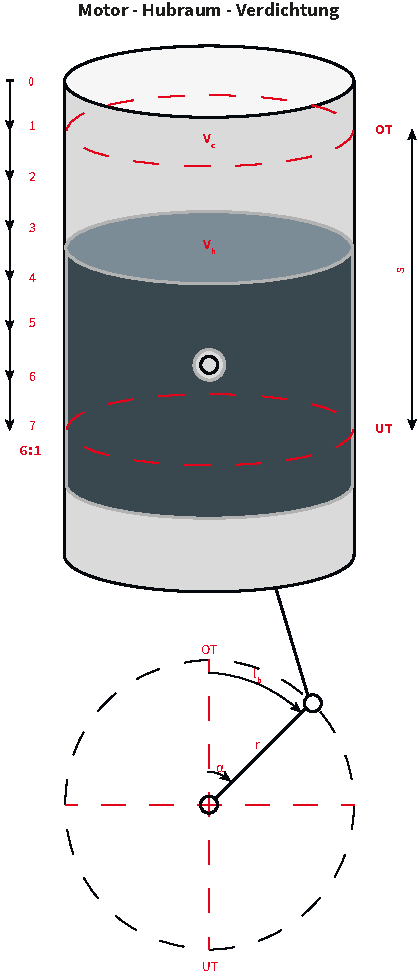
\includegraphics[width=.80\textwidth]{images/Motorzylinder_v2.pdf}%
  \caption{Motorzylinder_v2}%\label{fig:Motorzylinder_v2}%% anpassen
\end{figure}

%\newpage

%\chapter{Quellcode-files}
%% ---------------------------------
% Quellcode 'code/' in Latex speichern. 
% 'archiv/Quellcode-files.tex' 
% HTML, Python, Bash, C, C++, TeX 
% ju 17-Sep-2022 Quellcode-files.tex
% ---------------------------------
%

\section{Python_keywords}

%Python_keywords.py (\autoref{code:Python_keywords-1}).% Referenz
%
\lstset{language=Python}% HTML, Python, Bash, C, C++, TeX
\lstinputlisting[% anpassen
    caption={Quellcode in Python: Python_keywords.py}, %label={code:Python_keywords-1}
]{code/Python_keywords.py}% file

\newpage


%%%%%%%%%%%%%%%%%%%%%%%%%%%%%%%%%%%%%%%%%%%%%%%%%%

% Tabellen/

%\chapter{PDFs}
%% ju 28-Nov-2021 PDFs.tex

% -------
\section{Druck - Volumen - Temperatur}\label{sec:Druck-Volumen-Temp}\index{Druck-Volumen-Temp}
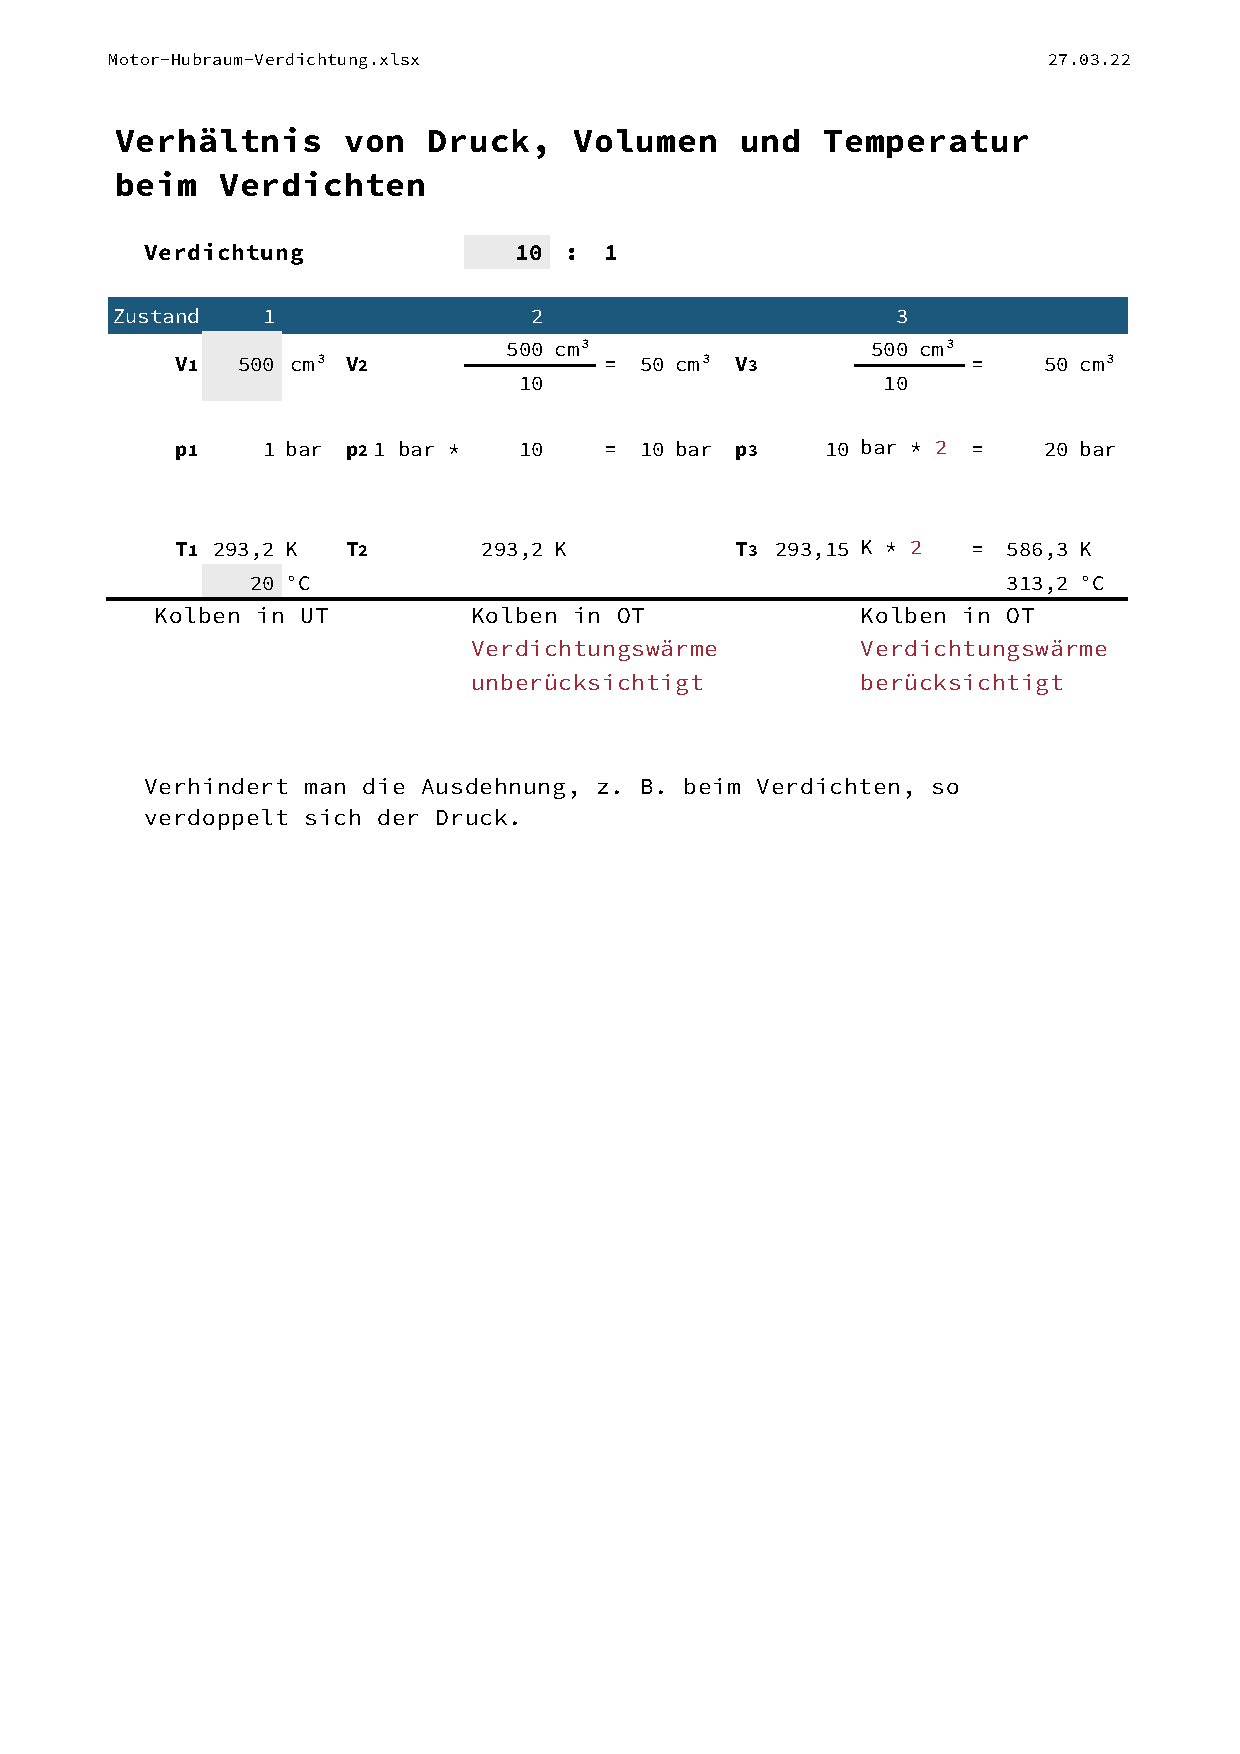
\includepdf[pages=-]{Tabellen/PDF/Druck-Volumen-Temp.pdf}

% -------
\section{Motor - Hubraum - Verdichtung}\label{sec:Motor-Hubraum-Verdichtung}\index{Motor-Hubraum-Verdichtung}
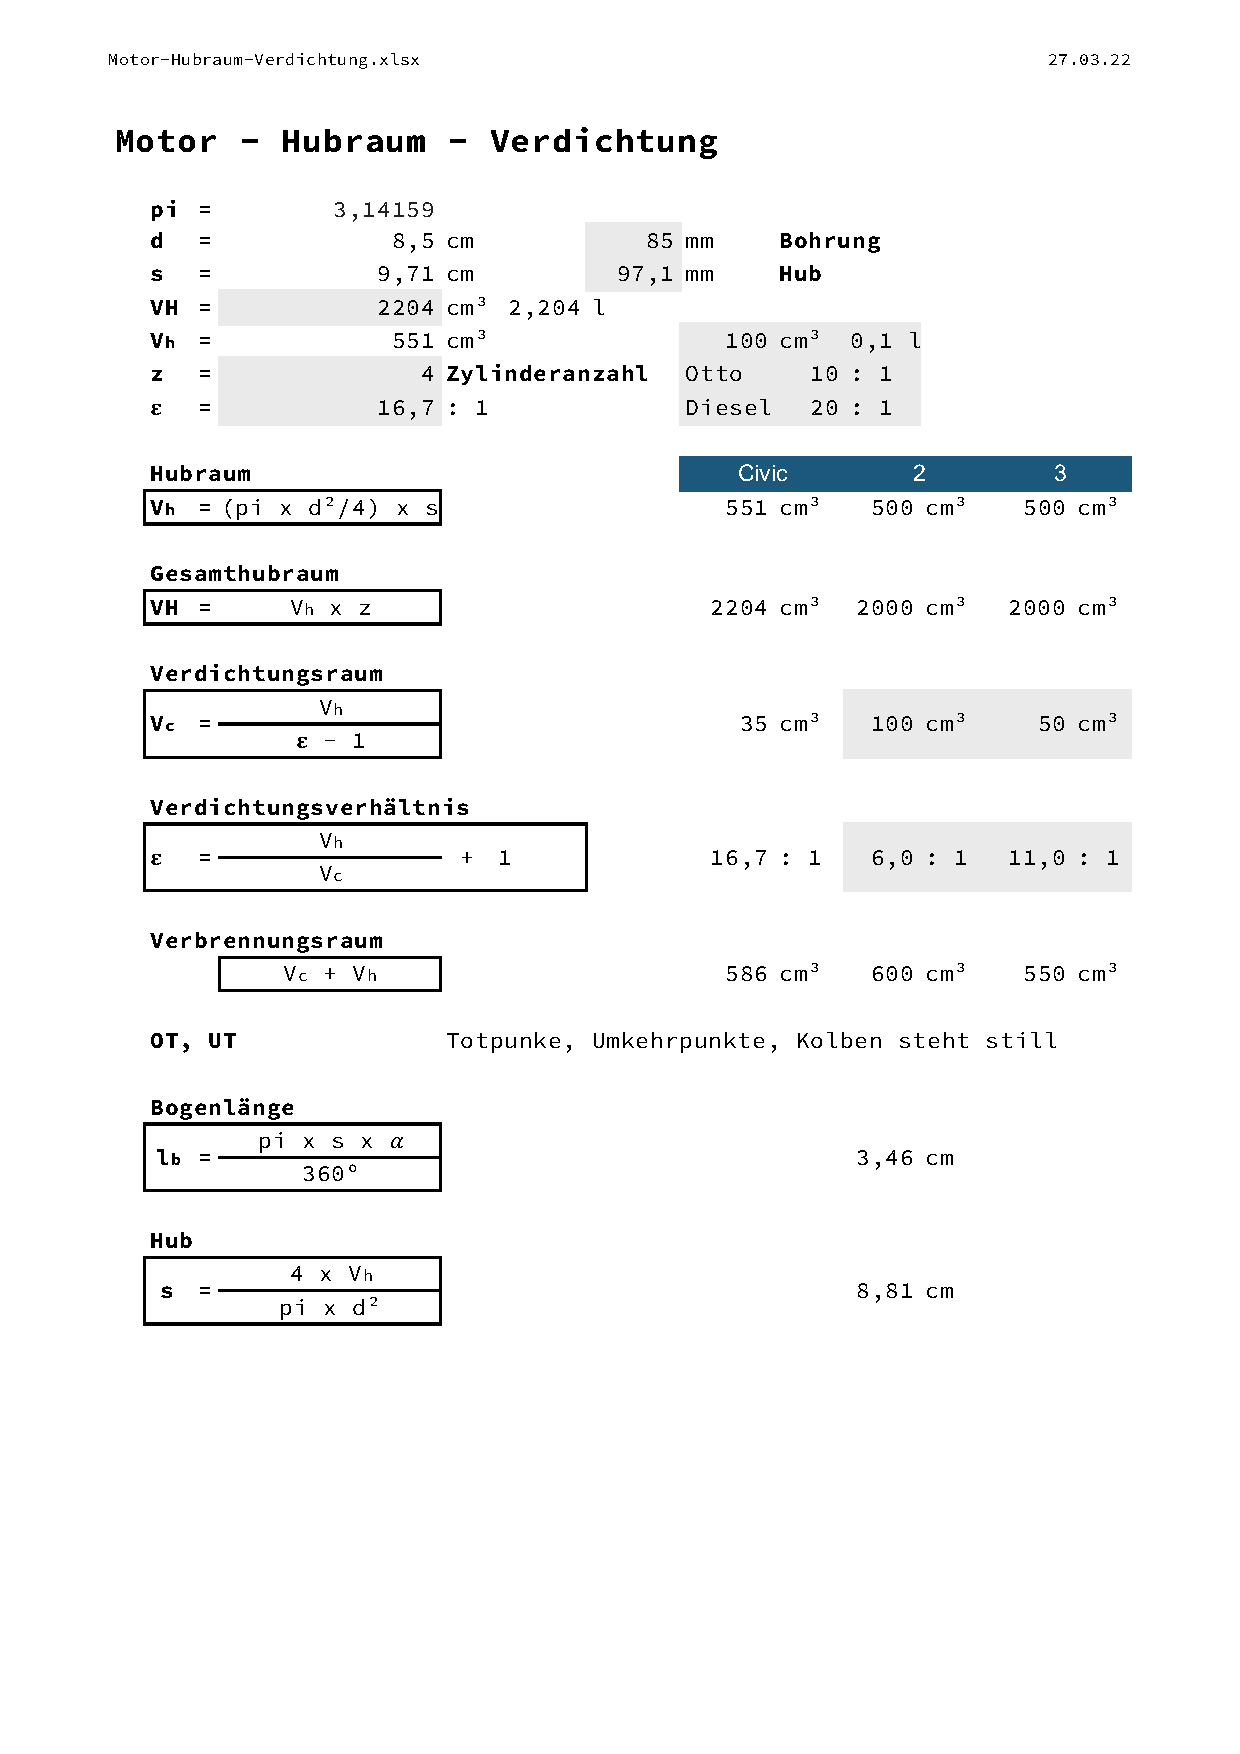
\includepdf[pages=-]{Tabellen/PDF/Motor-Hubraum-Verdichtung.pdf}






%%%%%%%%%%%%%%%%%%%%%%%%%%%%%%%%%%%%%%%%%%%%%%%%%%

% content/beispiele/tex/

%\chapter{Aufbau-der-Arbeit}
%%\chapter{Aufbau der Arbeit}

Jede Arbeit besteht in der Regel aus einer \textbf{Problemstellung}, einem \textbf{definitorischen Abschnitt}, der eigentlichen \textbf{Behandlung der Problemstellung} sowie einer \textbf{Zusammenfassung der zentralen Ergebnisse}.

\begin{description}

	\item[Einleitung] Im Zentrum des erstens Teils stehen die Darstellung des Themas der Arbeit und die genaue Auflistung der Fragestellungen (Wieso ist das Thema relevant?). Ebenso sollten schon einzelne Aspekte des Problems herausgearbeitet werden. Dabei ist es hilfreich, die zentralen Fragen aufzulisten, die im Rahmen der Arbeit beantwortet werden sollen.
	
	Außerdem sollte ein knapper Überblick gegeben werden, in welchen Schritten die Problembehandlung erfolgt: Hinführung zum Thema, Herleitung und Ausformulierung der Fragestellung, Abgrenzung des Themas (Angabe von Aspekten, die zum Thema gehören, aber ausgeklammert werden) und Aufbau der Arbeit (Begründung der Gliederung).
	
	\item[Grundlagen (definitorischer Teil)] Im zweiten Teil sollen zentrale Begriffe definiert und eingeordnet werden. Es geht dabei nicht darum, Definitionen aus Lexika zu suchen; stattdessen sollten problemorientierte Definitionen verwendet werden. Häufig können einzelne Begriffe unterschiedlich weit oder eng definiert werden, sodass auch eine Diskussion unterschiedlicher Definitionsansätze hilfreich sein kann, bevor eine für die weitere Arbeit verbindliche Definition gewählt wird. Zudem sollte ein Überblick über die in der Literatur vorhandenen Methoden bzw. Lösungsansätze, der aktuelle Stand der Technik und verwandte Arbeiten gegeben werden.
	
	\item[Hauptteil] Im Hauptteil der Arbeit (der in der Gliederung selbstverständlich nicht so zu benennen ist\ldots) erfolgt die eigentliche eigentliche Auseinandersetzung mit der Problemstellung. In diesem Teil kommt es darauf an, nicht nur Lehrbuchwissen zusammenzutragen, sondern die Problemstellung reflektiert zu bearbeiteten. Aussagen sollten durch herangezogene Literatur gestützt und belegt werden. Bitte darauf achten, in logischen, nachvollziehbaren Schritten vorzugehen.
	
	\item[Schlussbetrachtung] Die Antwort auf die in der Problemstellung aufgeworfenen Fragen soll kurz und prägnant zusammengefasst werden. Ebenso sollte ein Ausblick auf offen gebliebene Fragen sowie auf interessante Fragestellungen, die sich aus der Arbeit ergeben, gegeben werden. Eine kritische Betrachtung der eigenen Arbeit ist an dieser Stelle ebenfalls sinnvoll.

\end{description}

\noindent
Eine Sammlung unserer Tipps für das Schreiben von Ausarbeitungen befindet sich online unter \url{https://www.dcl.hpi.uni-potsdam.de/media/theses/}.

%\chapter{LaTeX-Beispiel-beamer}
%% ju 23-Jul-21
\section*{Einleitung}

\emph{Sonderzeichen}  wie <<\& oder \%>> müssen mit einem Backslash \verb|\& oder \%| maskiert werden, 
damit sie von LaTeX nicht als Befehle missverstanden werden.


\emph{Website} \footnote{\url{https://golatex.de/wiki/Hauptseite}} \verb|\footnote{\url{https://golatex.de/wiki/Hauptseite}}| 

\emph{PDF Datei einbinden} \verb|\includepdf[landscape=false]{images/logo.eps}| 
\includepdf[landscape=false]{images/logo.eps} 

\clearpage
\subsection*{Stand der Forschung}

Während die traditionelle Latexproduktion bereits hinreichend erforscht ist (\autoref{fig:latex}) \\
\verb|(\autoref{fig:latex})|, bleibt das wissenschaftliche Verständnis elektronischer Verarbeitungsprozesse dieses 
vielseitigen Materials weiterhin lückenhaft. 


\begin{figure}[!ht]% hier: !ht
	\centering
	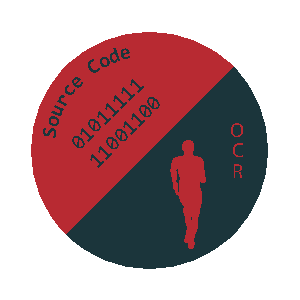
\includegraphics[width=0.25\textwidth]{images/logo.eps}
	\caption{Traditionelle Latexproduktion}\label{fig:latex}%
\end{figure}

\lstset{language=TeX}% C, TeX, Bash, Python 
\begin{lstlisting}[
	%caption={}, label={code:}%% anpassen
]
% Optionen
scale = Wert, Vergrösserungsfaktor
width/height = Wert für die Einstellung der Breite/Höhe
angle = Wert, Winkel (in Grad)
b = bottom - Seitenende 
t = top - Seitenanfang
h = here
p = page - komplette Seite  
% Abbildung
\begin{figure}[!ht]% hier: !ht
	\centering
	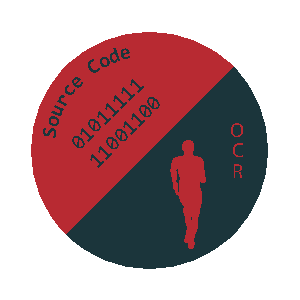
\includegraphics[width=0.25\textwidth]{images/logo.eps}
	\caption{Traditionelle Latexproduktion}\label{fig:latex}%
\end{figure}
\end{lstlisting}


\clearpage
\section*{Methodik}

Unter Zuhilfenahme der Formeln \autoref{eq:ekin} \verb|\autoref{eq:ekin}| und \autoref{eq:impuls} \verb|\autoref{eq:impuls}| werden wir 
diese Forschungslücke schließen.  
$E_{kin}$ \verb|$E_{kin}$| ist die kinetische Energie, $m$ \verb|$m$| die Masse und $\vec{v}$ \verb|$\vec{v}$| die Geschwindigkeit.

Wurzel $\sqrt{2}$ \verb|$\sqrt{2}$|

Bruch $\frac{\text{Zähler}}{\text{Nenner}}$ \verb|$\frac{\text{Zähler}}{\text{Nenner}}$|

\begin{equation}
	\label{eq:ekin}% 
	\sum E_{kin} = \sum E'_{kin}
\end{equation}

\begin{equation}
	\label{eq:impuls}% 
	\vec{v_1} - \vec{v_1'} = \frac{m_2}{m_1} (\vec{v_2'} - \vec{v_2})
\end{equation}

\lstset{language=TeX}% C, TeX, Bash, Python 
\begin{lstlisting}[
	%caption={}, label={code:}%% anpassen
]
% Mathe
\begin{equation}
	\label{eq:ekin}% 
	\sum E_{kin} = \sum E'_{kin}
\end{equation}
\end{lstlisting}


\clearpage
\section*{Ausblick}

Daraus ergeben sich gemäß (\autoref{tab:schritte}) \verb|(\autoref{tab:schritte})| folgende nächste Schritte, 
deren sequenzielle Ausführung von essenzieller Bedeutung ist.

\begin{table}[!ht]% hier: !ht
	\centering
	\begin{tabular}{@{}cl@{}}% lcr
		\toprule
		\textbf{Nr.} & \textbf{Vorgehen} \\
		\midrule
		1 & Aktuellen Forschungsstand recherchieren \\
		2 & Methoden entwickeln \\
		3 & Schlussfolgerung aufstellen \\
		\bottomrule
	\end{tabular}
	\caption{Nächste Schritte}\label{tab:schritte}
\end{table}

\clearpage
\lstset{language=TeX}% C, TeX, Bash, Python 
\begin{lstlisting}[
	%caption={}, label={code:}%% anpassen
]
% Tabelle
\begin{table}[!ht]% hier: !ht
	\centering
	\begin{tabular}{@{}cl@{}}% lcr
		\toprule
		\textbf{Nr.} & \textbf{Vorgehen} \\
		\midrule
		1 & Aktuellen Forschungsstand recherchieren \\
		2 & Methoden entwickeln \\
		3 & Schlussfolgerung aufstellen \\
		\bottomrule
	\end{tabular}
	\caption{Nächste Schritte}\label{tab:schritte}
\end{table}
\end{lstlisting}
%\chapter{Latex-install-Ubuntu}
%% letztes Update: 27-Jul-20
Quelle: Dr.~Uwe Ziegenhagen -- Anleitung zur TEX Live Installation

\section{TEX Live Download}\label{tex-live-download}

Download \footnote{\url{http://mirror.ctan.org/systems/texlive/tlnet}}

Download-texlive vgl.~(\autoref{code:Download-texlive}).

\lstset{language=C}% C, TeX, Bash, Python 
\begin{lstlisting}[%% anpassen
caption={Download-texlive},label={code:Download-texlive}
]
cd Downloads
tar xvfz install-tl-unx.tar.gz
cd install-tl-20200114
perl install-tl
perl install-tl -gui
\end{lstlisting}

\section{TeX Version}\label{tex-version}

tex --version

\section{TEX Live Installation}\label{tex-live-installation}

Install-texlive vgl.~(\autoref{code:Install-texlive}).

\lstset{language=C}% C, TeX, Bash, Python 
\begin{lstlisting}[%% anpassen
caption={Install-texlive},label={code:Install-texlive}
]
sudo apt install texlive texlive-latex-recommended texlive-fonts-recommended \
    texlive-latex-base texlive-base texlive-latex-extra texlive-lang-german

# Verbesserte Schriftarten bei T1-Kodierung
sudo apt-get install cm-super 
\end{lstlisting}

\section{Umgebungsvariablen für
Unix}\label{umgebungsvariablen-fuer-unix}

Umgebungsvariable vgl.~(\autoref{code:Umgebungsvariable}).

\lstset{language=C}% C, TeX, Bash, Python 
\begin{lstlisting}[%% anpassen
caption={Umgebungsvariable},label={code:Umgebungsvariable}
]
vi ~/.profile
# Datei 
PATH=/usr/local/texlive/2019/bin/x86_64-linux:$PATH; export PATH
MANPATH=/usr/local/texlive/2019/texmf-dist/doc/man:$MANPATH; export MANPATH
INFOPATH=/usr/local/texlive/2019/texmf-dist/doc/info:$INFOPATH; export INFOPATH

sudo vi /etc/manpath.config
# Datei 
MANPATH_MAP /usr/local/texlive/2019/bin/x86_64-linux \
  /usr/local/texlive/2019/texmf-dist/doc/man  
\end{lstlisting}

%\chapter{Mathe-Aufgaben}
%
\textbf{Aufgabe 1:} \enspace Jasmin hat ihre Freunde Nico, Laura und Anna zum Geburtstag eingeladen. Nico will nicht kommen, wenn Laura nicht kommt. Laura und Anna kommen beide oder kommen beide nicht. Aber Anna sagt: >>Wenn Nico und Laura beide nicht kommen, dann komme ich.<< Wer von den dreien wird unter diesen Bedingungen tatsächlich zum Geburtstag erscheinen?


\textbf{Aufgabe 2:} \enspace In der Anwaltsserie >>Suits<< (Staffel 4, Folge 1) kommt es zu Folgendem Gespräch zwischen Mike und seiner Sekräterin Amy.


\begin{enumerate}[label={\protect\ding{\value*}},start=192]
    \item Amy: >>Und wie lief dein Treffen mit dem geheimnisvollen Harvey Specter?<<
    \item Mike: >>Ein Arsch zu sein macht einen nicht geheimnisvoll.<<
    \item Amy: >>Na dann bist du ja ein ganz offenes Buch.<<
\end{enumerate}

Untersuchen Sie das Gespräch aussagenlogisch und prüfen Sie den Wahrheitswert von Amys Aussage.


\textbf{Aufgabe 3:} \enspace Formalisieren Sie die folgenden Aussagen und verneinen Sie sie anschließend (ohne das Wort nicht davor zu setzen) und übersetzen Sie wieder in Umgangssprache:

\begin{enumerate}[label=(\alph*)]
    \item Volksmund: >>Bei Nacht sind alle Katzen grau.<<
    \item Plakatwerbung: >>Wenn einer hochguckt, dann gucken alle.<<
    \item Gorbatschov: >>Wer zu spät kommt, den bestraft das Leben.<<
\end{enumerate}

\textbf{Aufgabe 4:} \enspace Wurzel

\begin{multicols}{3}
    \begin{enumerate}[label=(\alph*)]
        \item $\sqrt{169}$
        \item $\sqrt{0,36}$
        \item $\frac{\sqrt{45}}{\sqrt{80}}$
        \item $\sqrt{32}$
        \item $\sqrt{2}$
        \item $\sqrt{1,44}$
        \item $\sqrt{\frac{75}{12}}$
    \end{enumerate}
\end{multicols}
%\chapter{Mathe-Latex}
%\section{\textbf{Text Unterstreichen}}
    \underline{wichtiger Text} und \emph{kursiver Text} und \textbf{fetter Text}

 
\section{\textsc{Kapitaelchen}}  
    Text in Grossbuchstaben setzen durch \LaTeX
    \begin{itemize} % \item[] avoids bullet
        \item[] Einen längeren Satz\\ einrücken.
    \end{itemize}

\section{Vor- und Nachteile}
    \begin{tabular}[h]{ll}
        {\textbf{Vorteile}}   &  {\textbf{Nachteile}} \\
        Argument 1            &  Argument 2 \\
        Argument A            &  Argument B \\
    \end{tabular} 

\section{Summe}
    \begin{tabular}[h]{clrr}
        & Betrag &               &  $1.000,00$ \\
    $-$ & Skonto & $2\%$         &     $20,00$ \\
        \hline
    $=$ & $\sum$ &               &    $980,00$  
    \end{tabular} 
    
\section{Division Zinsen}
    $
        \frac{\text{ Betrag } \cdot \text{ Prozentsatz } \cdot \text{ Zeit } }{100 \cdot \text{ Zeitgröße }} 
        = \frac{12.597,90 \cdot 12 \cdot 20 \text{ T } }{100 \cdot 360} 
        = 83,99 \text{ \euro }
    $

    \begin{align*}
        \frac{\text{ Betrag } \cdot \text{ Prozentsatz } \cdot \text{ Zeit } }{100 \cdot \text{ Zeitgröße }} 
        = \frac{12.597,90 \cdot 12 \cdot 20 \text{ T } }{100 \cdot 360} 
        = 83,99 \text{ \euro }
    \end{align*} 

\section{Tabelle 2}
    \begin{table}[!ht]% hier: !ht 
        \begin{tabular}{@{}lcr@{}}
        \toprule 
        \textbf{Großbuchstaben} & \textbf{Kleinbuchstaben} & \textbf{Name}\\
        \midrule
        21 \euro & 22000 & 230.000 \\
        $31$ \euro & $32000$ & $330.000$ \\
        \bottomrule
        \end{tabular}
    \end{table}

\section{Checkliste}
    Meine Liste
    \begin{itemize} \itemsep -2pt  % reduce space between items
        \item[$\Box$]   Punkt 1
        \item[$\Box$]   Aufgabe 2 
    \end{itemize}

    \begin{itemize}[label=\checkmark] \itemsep -2pt
        \item Check 1
        \item Check 2   
    \end{itemize}

\section{\textcolor{rot5}{Nenne 4x Lerzielstufen (Taxonomien)}}
    \begin{enumerate}[label={\protect\ding{\value*}},start=192]
        \item Reproduktion
        \item Reorganisieren
        \item Transfer
        \item Kreativ
    \end{enumerate}

\section{Wurzel berechnen}
    \begin{multicols}{3}
        \begin{enumerate}[label=(\alph*)]
            \item $\sqrt{169}$
            \item $\sqrt{0,36}$
            \item $\frac{\sqrt{45}}{\sqrt{80}}$
        \end{enumerate}
    \end{multicols}

\section{Aufgabe Logik}
    Formalisieren Sie die folgenden Aussagen und verneinen Sie sie anschließend (ohne das Wort nicht davor zu setzen) und übersetzen Sie wieder in Umgangssprache:

    \begin{enumerate}[label=(\alph*)]
        \item Volksmund: >>Bei Nacht sind alle Katzen grau.<<
        \item Plakatwerbung: >>Wenn einer hochguckt, dann gucken alle.<<
        \item Gorbatschov: >>Wer zu spät kommt, den bestraft das Leben.<<
    \end{enumerate}

\section{Quotientenregel}
    \begin{itemize} % \item[] ohne bullet
        \item[] $\left(\frac{u}{v}\right)^{\prime} = \frac{u^{\prime} \cdot v-u \cdot v^{\prime}}{v^{2}}$
        
        \item[] $\frac{\text{ Ableiten } \cdot \text{ Stehen lassen } - \text{ Stehen lassen } \cdot \text{ Ableiten }}{\text{ Nenner}^2}$
    \end{itemize}

    
\section{Logarithmus}
    \begin{align}
        ln(a \cdot b)   &= ln(a) + ln(b) \\
        ln(\frac{a}{b}) &= ln(a) - ln(b) \\
        ln(a^b)         &= b \cdot ln(a)
    \end{align}

    \newpage
\section{\LaTeX - Assistent}
    Formeleditor~\footnote{\url{https://www.matheretter.de/rechner/latex}}
    \begin{align}
        \text{ Matrix }       &= \begin{pmatrix} a & b \\ c & d \end{pmatrix} \\
        \text{ Vektor }       &= \begin{pmatrix} x\\y \end{pmatrix} \\
        \text{ Vektorbuchstabe } &= \vec{x} \\
        \text{ Wurzel }       &= \sqrt[n]{a} \text{ Potenz } a^{b} \\
        \text{ Bruch }        &= \frac{a}{b} \\
        \text{ Log }          &= \log_{b}{a} \\
        \text{ Summe }        &= \sum \limits_{n=0}^{\infty} \\
        \text{ Index }        &= x_{1,2} \\
        \text{ Klammern }     &= \left\{x, y\right\} \\
        \text{ Alphabet kl. } &= +\\%α β γ δ ε ζ η θ ι κ λ μ ν ξ ο π ρ σ τ υ φ χ ψ ω \\
        \text{ Alphabet gr. } &= +\\%Α Β Γ Δ Ε Ζ Η Θ Ι Κ Λ Μ Ν Ξ Ο Π Ρ Σ Τ Υ Φ Χ Ψ Ω \\
        \text{ Element }      &= \in \notin \sum \quad \prod \quad () \quad \to \quad \infty\\
        \text{ Mengen }       &= \mathbb{N} \mathbb{Z} \mathbb{Q} \mathbb{R} \mathbb{I} \mathbb{C} \mathbb{L} \\
        \text{ Relation }     &= < > \geq \leq \neq \subset \subseteq \approx \in \supset \supseteq \notin \\
        \text{ Pfeile }       &= +\\%\rightarrow \leftarrow \Longleftrightarrow \Longrightarrow \Longleftarrow \\
    \end{align}

\section{Formeln in einer Zeile}
    $
        u = \bar{u} + \epsilon \cdot u_1 \quad
        v = \bar{v} + \epsilon \cdot v_1 \quad
        w = \bar{w} + \epsilon \cdot w_1 \quad
    $

    $
        \left( \begin{array}{rrr}
            1 & 0 & 0 \\                                              
            0 & 1 & 0 \\
            0 & 0 & 1 \\                                              
        \end{array}\right)
    $

\section{Sonderzeichen}
    \textbackslash \{...\} \$ \& \# \textdegree \^{} \_ \textasciitilde \%

\section{Währungszeichen}
    \euro 100 \textdollar 100 \textsterling 100 $1.000,00 \text{ \euro }$ 1.000,00 \euro

\section{Leerzeichen}
\begin{itemize} % \item[] avoids bullet
    \item[] [a\,b] ($0.16667em$)
    \item[] [a\:b] ($0.2222em$)
    \item[] [a\enspace b] ($0.5em$)
    \item[] [a\quad b] ($1em$)
    \item[] [a\hspace{5em} b] (5em)
\end{itemize}

\newpage
\section{Griechisches Alphabet}
    \begin{table}[!ht]% hier: !ht 
        \begin{tabular}{@{}ccl@{}}
        \toprule 
        \textbf{Großbuchstaben} & \textbf{Kleinbuchstaben} & \textbf{Name}\\
        \midrule
        A & $\alpha$ & Alpha\\
        B & $\beta$ & Beta\\
        $\Gamma$ & $\gamma$ & Gamma \\
        $\Delta$ & $\delta$ & Delta\\
        E & $\epsilon$, $\varepsilon$ & Epsilon\\
        Z & $\zeta$ & Zeta\\
        H & $\eta$ & Eta\\
        $\Theta$ & $\theta$, $\vartheta$ & Theta\\
        I & $\iota$ & Iota\\
        K & $\kappa$, $\varkappa$ & Kappa\\
        $\Lambda$ & $\lambda$ & Lambda\\
        M & $\mu$ & My\\
        N & $\nu$ & Ny\\
        $\Xi$ & $\xi$ & Xi\\
        O & o & Omikron\\
        $\Pi$ & $\pi$, $\varpi$ & Pi\\
        P & $\rho$, $\varrho$ & Rho\\
        $\Sigma$ & $\sigma$, $\varsigma$ & Sigma\\
        T & $\tau$ & Tau\\
        Y & $\upsilon$ & Ypsilon\\
        $\Phi$ & $\phi$, $\varphi$ & Phi\\
        X & $\chi$ & Chi\\
        $\Psi$ & $\psi$ & Psi\\
        $\Omega$ & $\omega$ & Omega\\
        \bottomrule
        \end{tabular}
    \end{table}

\section{Tabelle 3}
    Tabellengenerator~\footnote{\url{https://www.tablesgenerator.com/}} 
    und Rechner~\footnote{\url{https://www.matheretter.de/rechner/latex}}

    \begin{multicols}{2}
        \begin{tabular}[h]{ll|l}
            &  A     & B     \\ 
        \hline
        1)* &  $a_1$ & $b_1$ \\
        2)  &  $a_2$ & $b_2$ \\
        3)  &  $a_3$ & $b_3$ 
        \end{tabular}
        
        \columnbreak% Spalte
        *Beachte: $\sqrt[n]{x} = x^\frac{1}{n}$       
    \end{multicols}

\section{Tabelle und Grafik}
    \begin{multicols}{2}
        \begin{tabular}[h]{l|c|r}
            Spalte 1 & Spalte 2 & Spalte 3 \\
            \hline
            heise & tipps & tricks \\
        \end{tabular}    

        \columnbreak% Spalte

        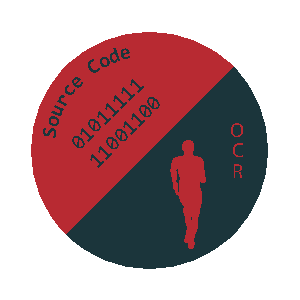
\includegraphics[width=2.0cm]{images/logo.eps}% Logo   
    \end{multicols}  

\newpage
\section{Farben}
    \begin{testcolors}[rgb,cmyk,HTML,gray]
        \testcolor{black}
        \testcolor{white}
        \testcolor{darkgray}
        \testcolor{gray}
        \testcolor{lightgray}
        \testcolor{red}
        \testcolor{green}
        \testcolor{blue}
        \testcolor{cyan}
        \testcolor{magenta}
        \testcolor{yellow}
        \testcolor{brown}
        \testcolor{lime}
        \testcolor{olive}
        \testcolor{orange}
        \testcolor{pink}
        \testcolor{purple}
        \testcolor{teal}
        \testcolor{violet}
        \testcolor{rot5}
        \testcolor{blau5}  
        \testcolor{grau2}    
        \testcolor{orange}                       
    \end{testcolors}
    
\section{Farbenfolgen}
    \definecolorseries{test}{rgb}{step}[rgb]{.95,.85,.55}{.17,.47,.37}
    \definecolorseries{test}{hsb}{step}[hsb]{.575,1,1}{.11,-.05,0}
    \definecolorseries{test}{rgb}{grad}[rgb]{.95,.85,.55}{3,11,17}
    \definecolorseries{test}{hsb}{grad}[hsb]{.575,1,1}{.987,-.234,0}
    \definecolorseries{test}{rgb}{last}[rgb]{.95,.85,.55}[rgb]{.05,.15,.55}
    \definecolorseries{test}{hsb}{last}[hsb]{.575,1,1}[hsb]{-.425,.15,1}
    \definecolorseries{test}{rgb}{last}{red!50}{blue}
    \definecolorseries{test}{hsb}{last}{yellow!50}{black}
    \definecolorseries{test}{cmy}{last}{orange!50}{green}

    \resetcolorseries[12]{test}
    \rowcolors[\hline]{1}{test!!+}{test!!+}
    \setlength{\tabcolsep}{5mm} % Abstände zwischen den Spalten
    \begin{tabular}[h]{c||c||c||c||c||c||c||c||c||c}
        $S_1$ & $S_2$ & $G_1$ & $G_2$ & $L_1$ & $L_2$ & $L_3$ & $L_4$ & $L_5$ \\
        \hline \hline
        \number\rownum & \number\rownum & \number\rownum & \number\rownum & \number\rownum & \number\rownum & \number\rownum & \number\rownum & \number\rownum \\
        \number\rownum & \number\rownum & \number\rownum & \number\rownum & \number\rownum & \number\rownum & \number\rownum & \number\rownum & \number\rownum \\
        \number\rownum & \number\rownum & \number\rownum & \number\rownum & \number\rownum & \number\rownum & \number\rownum & \number\rownum & \number\rownum \\
        \number\rownum & \number\rownum & \number\rownum & \number\rownum & \number\rownum & \number\rownum & \number\rownum & \number\rownum & \number\rownum \\
        \number\rownum & \number\rownum & \number\rownum & \number\rownum & \number\rownum & \number\rownum & \number\rownum & \number\rownum & \number\rownum \\
        \number\rownum & \number\rownum & \number\rownum & \number\rownum & \number\rownum & \number\rownum & \number\rownum & \number\rownum & \number\rownum \\
        \number\rownum & \number\rownum & \number\rownum & \number\rownum & \number\rownum & \number\rownum & \number\rownum & \number\rownum & \number\rownum \\
        \number\rownum & \number\rownum & \number\rownum & \number\rownum & \number\rownum & \number\rownum & \number\rownum & \number\rownum & \number\rownum \\
        \number\rownum & \number\rownum & \number\rownum & \number\rownum & \number\rownum & \number\rownum & \number\rownum & \number\rownum & \number\rownum \\
        \number\rownum & \number\rownum & \number\rownum & \number\rownum & \number\rownum & \number\rownum & \number\rownum & \number\rownum & \number\rownum \\
        \number\rownum & \number\rownum & \number\rownum & \number\rownum & \number\rownum & \number\rownum & \number\rownum & \number\rownum & \number\rownum \\
        \number\rownum & \number\rownum & \number\rownum & \number\rownum & \number\rownum & \number\rownum & \number\rownum & \number\rownum & \number\rownum \\
        \number\rownum & \number\rownum & \number\rownum & \number\rownum & \number\rownum & \number\rownum & \number\rownum & \number\rownum & \number\rownum \\
        \number\rownum & \number\rownum & \number\rownum & \number\rownum & \number\rownum & \number\rownum & \number\rownum & \number\rownum & \number\rownum \\
        \number\rownum & \number\rownum & \number\rownum & \number\rownum & \number\rownum & \number\rownum & \number\rownum & \number\rownum & \number\rownum \\ 
    \end{tabular}
%\chapter{Sprachlich-formale-Aspekte}
%%\chapter{Sprachlich-formale Aspekte}

Wissenschaftliche Ausarbeitungen dienen der Wissensvermittlung -- es ist überaus wichtig, Lesenden die Informationsaufnahme möglichst einfach zu machen, Inhalte logisch zu gliedern und in guter sprachlicher Form darzustellen.


\section{Textverständlichkeit}

Der Text ist logisch aufzubauen und so zu formulieren, dass er auch für den nicht an der Durchführung der Arbeit beteiligten Lesenden verständlich und nachvollziehbar ist. Die behandelten Themen müssen leicht erkennbar sein. Größere Abschnitte sollten einen kurzen Überblick über ihre Inhalte geben. Die Verständlichkeit des Textes kann durch die Verwendung von kurzen Sätzen, einer einfachen, aber fachsprachlich korrekten Wortwahl und durch die Vermeidung von Füllworten und überflüssigen Fremdworten wesentlich erhöht werden.

\begin{itemize}
\item Keine Prosa, sondern präzise Begriffe und Sätze!
\item Eine einheitliche Terminologie verwenden, damit Begriffe wiedererkannt werden können.
\item Zentrale Begriffe klären und die Arbeit für interessierte Laien verständlich halten.
\item Pure Textblöcke, die sich über mehrere Seiten erstrecken, sind ein Zeichen für mangelnde strukturelle Leseunterstützung. Weiter unterteilen oder variantenreichere Inhaltsarten (Schriftarten, Listen, Diagramme, Tabellen, \ldots) einsetzen.
\item Das schnelle überfliegen des Textes und das Springen in der Arbeit muss aktiv unterstützt werden. Lesende müssen jederzeit die wesentlichen gerade diskutierten Themen schnell erkennen und auch bestimmte vorher schon einmal gelesene Fakten schnell wiederfinden können.
\item Kurz einen Gesamtüberblick (Einordnung ins >>große Bild<<, eine Tabelle) geben und dann tiefer in die Details. Z. B. vor dem Start einer Reihe von Subsections die verschiedene Ausprägungen eines Sachverhalts diskutieren, diese Sachverhalte vorher alle aufzählen und kurz erläutern.
\item Fremdworte/Fachbegriffe nicht einfach ohne weitere Erläuterung verwenden und als bekannt voraussetzen. Selbst wenn der Begriff etabliert und bekannt scheint -- das ist oft auch nur in einem Teilgebiet (der Informatik) so. Deshalb generell Fachbegriffe und Fremdworte erläutern.
\item Die einzelnen Abschnitte sollten entsprechend auf einander verweisen. Überleitungen und Zusammenfassungen zwischen Kapiteln sind hilfreich.
\item Zu Beginn eines Kapitels ist eine Übersicht über dessen Inhalt sinnvoll. Am Ende eines Kapitels kann eine Überleitung zum nächsten Kapitel helfen, den roten Faden aufzuzeigen.
\item Gute Überschriften, vielseitige Präsentation der Inhalte (Diagramme, Tabellen, Auflistungen, \ldots) und aussagekräftige Inhaltsunterschriften verwenden.
\item Durch eine Kombination aus Text und Bild lassen sich komplexe Sachverhalte vereinfacht darstellen und verständlich vermitteln.
\item Verwendet sprechende Titel für Kapitel/Sections/\ldots! Nicht einfach nur >>Aufbau<<, >>Mechanismen<<, >>Dritter Schritt<<, etc. Man sollte nicht erst den Text lesen müssen, um den Kontext zu verstehen. Viel besser: >>Aufbau einer Ausführungsumgebung für Microservices<<, >>Mechanismen zur Fehlervermeidung und Fehlerbeseitigung<<, >>Dritter Schritt: Implementierung der Schnittstellen zwischen Diensten<<.
\item Statt in der Textform z. B. >>mittels einerseits \ldots andererseits<<,\\>>erstens\ldots zweitens\ldots drittens<< o. ä. lieber Aufzählungszeichen verwenden. Dies unterstützt die Lesbarkeit teilweise enorm.
\item Möglichkeiten zur Hervorhebung (z. B. Fettdruck) und Textstrukturierung (Gedankenstriche, Klammern, Semikolon, Doppelpunkt, \ldots) nutzen.
\end{itemize}



\section{Ausdruck \& Stil}

Eine wissenschaftliche Ausdrucksweise ist sachlich, präzise und bemüht sich um Objektivität. Die Verwendung umgangssprachlicher Ausdrücke, schwammiger Formulierungen und übertriebener literarischer Stilmittel (z. B. Verwendung von Synonymen) stören die wissenschaftliche Ausdrucksweise.

\begin{itemize}
\item Umgangssprachliche Formulierungen vermeiden (>>von vorneherein<<, >>wird es richtig teuer<<, >>ziemlich simpel<<, >>Gehen wir das ganze einmal durch<<, >>zum Laufen zu bringen<<, >>sprich\ldots<<, >>Fazit: \ldots<<, >>Ich habe mir gedacht,\ldots<<)
\item Komponenten nicht personifizieren (>>der JBoss/er<<, >>die Apaches<<, >>JBosse<<).
\item    Vermeidet das Wort >>offensichtlich<<. Das wirkt, als hieltet ihr die Lesenden für dumm.
\item    Vermeidet Füllwörter wie >>sehr<<. Wenn etwas >>sehr wichtig<< ist, dann sind in der Schriftsprache Worte wie >>zentral<<, >>fundamental<<, >>essentiell<<, etc. eleganter.
\item    Worte wie >>sehr<<, >>relativ<<, >>ziemlich<<, >>quasi<<, >>gewissermaßen<< sind in den allermeisten Fällen überflüssig und ungenau.
\item    Die Begriffe, für die Demonstrativpronomen (dieser/jener/welcher) Stellvertreter sind, müssen eindeutig erkennbar sein.
\item    Nicht zu umständliche Stellvertreterausdrücke verwenden (>>der zur Diskussion stehende Sachverhalt<<, >>die vorbezeichneten Gegenstände<<, etc.) -- da müssen Lesende viel zu viel nachdenken (und erstmal den Lesefluss stoppen und nachgucken, welche drei Sachen eigentlich gemeint sind).
\item    Nicht verschiedenste Synonyme für ein und denselben Begriff verwenden -- insbesondere, wenn der Begriff etabliert ist (Negativbeispiel: >>künstliche neuronale Netze<<, >>artifizielle Netze<<, >>die in Rede stehenden Netze<<, >>ebenjene Netze<<, >>die beschriebenen Netze<<)
\end{itemize}



\section{Rechtschreibung \& Grammatik}

Mindestens ebenso wichtig wie die Verständlichkeit ist die sprachliche Korrektheit. Ausarbeitungen müssen hinsichtlich Rechtschreibung, Grammatik, Satzbau und Zeichensetzung ohne Fehler sein. Ein nennenswerter Fehleranteil wird oft als Indikator für mangelnde Sorgfalt und Ernsthaftigkeit der Arbeit gewertet. Solche Arbeiten werden nicht anerkannt auch nicht als Vor-Version!).

\begin{itemize}
\item Alles, was die Rechtschreibkontrolle nicht kennt, ist entweder falsch geschrieben oder muss als Fremdwort, Eigenname, \verb|\code| etc. hervorgehoben sein.
\item Es empfiehlt sich generell, Freunde, Kommilitonen, und eine Software zur Prüfung der Rechtschreibung \& Grammatik nochmal auf den Text schauen zu lassen. Als Autor bekommt man schnell einen Tunnelblick und sieht die Fehler nicht mehr.
\item Beachtet schwierige Wörter. >>zum einen<<, >>zum anderen<<, >>des Weiteren<<
\item Regeln für das Setzen von Bindestrichen: Deutsch > immer (>>Hasso-Plattner-Institut<<), Englisch > in der Regel nicht (>>Hasso Plattner Institute<<), Deutsch+Englisch > kombiniert (>>Java EE-Sicherheitsmodell<<). Im Deutschen kommt es äußerst selten vor, dass Worte weder Bindestrich haben noch zusammengeschrieben werden können. Es heißt z. B. nicht >>Download Modus<<, sondern >>Download-Modus<< oder (da Download im Duden steht) >>Downloadmodus<<.
\item Zu einem >>einerseits<< muss es ein >>andererseits<< geben, zu einem >>erstens<< auch ein >>zweitens<<, zu einem >>sowohl<< auch ein >>als auch<<, usw.
\end{itemize}

Schreibung von Zahlen (deutsch):

\begin{itemize}
\item Zahlen von eins bis zwölf werden in der Regel ausgeschrieben. Ansonsten nur ein- und zweisilbige Zahlwörter (hundert, tausend, \ldots)
\item Vor Zeichen, Abkürzungen von Maßen, Gewichten, Geldsorten usw. ist die Zahl in Ziffern zu schreiben: 3 km; 7,4 kg; 6 EUR. Steht statt der Abkürzung die entsprechende Vollform, kann man sowohl in Ziffern als auch in Buchstaben schreiben: 11 Kilometer/elf Kilometer; 2 Euro/zwei Euro.
\item Die Zahlen von 13 an können -- sofern sie Übersichtlich sind -- auch ausgeschrieben werden.
\item Im IT-Bereich gibt es sehr oft einen Unterschied zwischen 0 (dem Zahlenwert) und null (dem Nullwert/NIL, Fehlen eines Wertes)!
\item Zahlen sollten zur besseren Lesbarkeit in Dreiergruppen gegliedert werden, und zwar sowohl links als auch rechts des Dezimaltrennzeichens. Laut ISO 80000 soll das Tausendertrennzeichen ein schmales Leerzeichen sein, niemals ein Komma, Punkt oder irgendein anderes Zeichen. Zahlen sollten (außer bei tabellarischer Darstellung) erst ab fünf Stellen untergliedert werden.
\item Sätze nie mit Konjunktionen (>>und<<, >>oder<<, >>aber<<, sondern) beginnen. Konjunktionen sind -- wie der Name schon sagt -- Verbindungswörter und stellen die syntaktische Verbindung zwischen Wörtern, Satzteilen oder Sätzen her.
\end{itemize}


\section{Grafiken, Tabellen \& Codeausschnitte}

Jede Fließumgebung (Grafiken, Graphen, Diagramme, Tabellen, Codeausschnitte, \ldots) muss beschriftet sein (>>captions<<).

\begin{itemize}
\item Die Beschreibungen der Abbildungen, Tabellen, Diagramme, Quellcode, etc. müssen jene auch ohne Kontext beschreiben -- erläutern, was man alles sehen und erkennen kann. So muss man beim Betrachten nicht zurück in den Fließtext springen.
\item In jeder Beschriftung müssen folgende Fragen beantwortet werden: Was ist dargestellt? Welche Besonderheiten sind zu erkennen? Welche Rückschlüsse ergeben sich daraus für den momentan behandelten Sachverhalt?
\item Die Achsen von Diagrammen ordentlich beschriften (Metrik und Einheiten). Bei Vergleichen angeben, ob große oder ob kleine Werte besser sind. Fehlerbalken verwenden.
\item Wenn Text in den Abbildungen auf Englisch ist, man aber einen deutschen Text schreibt: Entweder den Text in der Abbildungen übersetzen, oder die Bildunterschrift so gestalten, dass man das auch verstehen kann, wenn man kein Englisch kann.
\item Bilder so skalieren, dass die Textgrößen verschiedener Abbildungen etwa konsistent sind und nicht sehr viel größer (oder kleiner) als die normale Textschriftgröße.
\item Grafiken, Tabellen etc. müssen auch im Text referenziert werden um die Verbindung zwischen Text und Abbildungen herzustellen.
\end{itemize}

\section{weitere wichtige Formalien}

Bei den Formalien gibt es verschiedene Möglichkeiten -- die Grundregel sollte jedoch sein: Hauptsache einheitlich, Übersichtlich und systematisch!

\begin{itemize}
\item Fachbegriffe, Produkt-/Eigennamen und fremdsprachlichen Begriffen (z. B. Java EE, Java Virtual Machine, Enterprise Services, Application Client Container) bei der ersten Verwendung kenntlich machen (z. B. mittels \verb|\emph|) und auch eine kurze Erläuterung mit hinzufügen. Oft lässt sich das Erläutern eines Fremdworts/Fachbegriffs leicht durch eine Übersetzung implementieren; manchmal aber auch nicht: Dann muss ein Nebensatz, eine Fußnote o. ä. investiert werden, um den Fachbegriff/das Fremdwort genauer zu erklären. Danach kann auch das Fremdwort normal verwendet werden.
\item Bei englischen Begriffen, die leicht durch deutsche Begriffe ersetzt werden können, dies bitte auch tun (z. B. >>Interface<< vs. >>Schnittstelle<<, >>Button<< vs. >>Schaltfläche<<).
\item Abkürzungen sind grundsätzlich bei ihrer ersten Verwendung einmal aufzuschlüsseln. Auch Begriffe, die im Glossar erwähnt sind, sind bei der ersten Verwendung in der Arbeit noch einmal kurz zu erläutern (z. B. Pan- und Pitch-Gesten).
\item Bei Verwendung von Unterpunkten müssen mindestens zwei Unterpunkte vorhanden sein (also >>2.<< >>2.1<< >>2.2<< \ldots >>3.<< statt >>2<< >>2.1<< >>3<<).
\item Eine Section, auf die sofort eine Subsection (ohne Text dazwischen) folgt, ist unschön.
\item Bei Nennung von Produkten die URL der Bezugsquelle als Fußnote angeben.
\item URLs nicht in den Fließtext integrieren, sondern als Fußnote oder ggf. als Referenz darauf verweisen (sonst unterbrechen sie durch ihre Länge den Lesefluss). Bei Verwendung von LaTeX die URLs immer auch in die \verb|\url|-Umgebung einfügen.
\item Schreiben in der ersten Person Singular vermeiden. >>Ich<< ist üblicherweise nur akzeptabel, wenn es um eigene Leistungen/Beiträge geht.
\item Aufzählung einzelner Begriffe nur machen, wenn sie in der Auflistung noch etwas genauer erklärt werden. Ansonsten einfach als Fließtext hintereinander aufschreiben.
\item Sind Subsections wirklich immer nötig? Oder tut es vielleicht auch eine einfache Auflistung?
\item Keine zusätzlichen Formatierungen in Überschriften verwenden.
\end{itemize}



\section{spezielle Hinweise für Ausarbeitungen, die mit LaTeX bearbeitet werden}

\begin{itemize}
\item Absätze nicht mit \verb|\\| trennen, sondern durch eine Leerzeile. Die beiden Sachen sehen im erstellten Dokument unterschiedlich aus (sonst werden z. B. die Absätze nicht eingerückt).
\item Für Gedankenstriche bitte \verb|--| benutzen (doppeltes Minus).
    Mithilfe einer \verb|~| (Tilde) kann ein geschütztes Leerzeichen (engl. no-break space) eingefügt werden, dass einen automatischen Zeilenumbruch an dieser Position verhindert (bzw. verzögert) und dadurch die Lesbarkeit verbessert (z. B. \verb|123~kg|, \verb|3~Liter|, \verb|DB~Systel|, \verb|S.~42~ff.| oder auch zur Umbruchsteuerung bei Titel-Angaben).
\item Bei allen Quellen, die im Quellenverzeichnis auftauchen sollen, muss irgendwo eine Referenz darauf existieren (kein \verb|\NoCite|!).
\item URLs bitte in die \verb|\url|-Umgebung einfügen, möglichst in eine Fußnote (\verb|\footnote|) packen, den Seitentitel nennen und ggf. das Abrufdatum angeben.
\item Kein \verb|\emph| o. ä. in Überschriften verwenden.
\item Literaturverzeichnis: Als *.bib-Datei!
\item Bei Firmen-/Organisationsbezeichnungen im author-Feld die sich aus mehreren Wörtern zusammensetzen (und die keine Vornamen/Nachnamen sind) diese separat in \verb|{}| packen. Zum Beispiel \verb|{{Microsoft Corporation}}| (damit sie nicht als Vor-/Nachname formatiert werden).
\item Bei mehreren Autoren diese nicht mit Komma voneinander trennen, sondern mit and.
\end{itemize}



\section{Korrektur \& Abgabe}

Eine gute schriftliche Ausarbeitung braucht eine gute Argumentation und eine gute Schlussüberarbeitung. Diese sind jedoch nicht nach ersten Niederschrift fertig -- daher sind mehrere Überarbeitungen vor Abgabe der Endfassung unbedingt notwendig. Kurze und präzise Formulierungen entwickelt man nicht beim ersten Nachdenken über ein Problem. Logikfehler oder fehlende Argumente fallen nicht sofort auf.

\begin{itemize}
\item Den Text mehrfach lesen und überarbeiten.
\item Wiederholungen beseitigen, Abschnitte eventuell umstellen, umformulieren, Brüche glätten, Teile verbinden, Aussagen präzisieren, an der Sprache feilen.
\item Den roten Faden durchgängig kenntlich machen, die Fragestellung und Argumentation schärfen, deren Nachvollziehbarkeit überprüfen.
\item Möglichst auch noch einmal eine (externe) Rechtschreibkontrolle zu Rate ziehen -- eine korrekte Rechtschreibung und Grammatik sind ein Muss!
\item Ebenfalls solltet ihr vor der Abgabe eines Dokuments noch einmal (gründlich) nachschauen, ob alles so aussieht, wie es soll passt das Layout, wurden alle (gravierenden) overfull-Boxes beseitigt, sind die Referenzen ordentlich gesetzt, ist das Literaturverzeichnis vorhanden usw.
\item Wichtig ist auch, dass ihr euch jeden einzelnen Eintrag im Literaturverzeichnis noch einmal anschaut -- sind notwendigen Angaben alle dargestellt, ist die Autorenliste korrekt, sieht man bei Online-Quellen auch die Adresse etc.
\end{itemize}

\section{Drucken \& Binden}

Nach dem Schreiben der Abschluss-Arbeit muss diese noch gedruckt und gebunden werden. Damit das möglichst hochwertig, schnell und preiswert geschehen kann, solltet ihr folgende Dinge beachten:

\begin{itemize}
\item \emph{Papierstärke} Für den Ausdruck bitte ordentliches Papier verwenden (so, dass man die Rückseite nicht durchschimmern sieht). Um professionell zu wirken, sollte Papier mit mind. $100~g/m^2$ gewählt werden.
\item \emph{Bindung} Wir raten dazu, beim Binden ein >>Softcover mit Aufdruck auf der Vorderseite<< zu wählen; ein Hardcover geht natürlich auch, ist allerdings etwas teurer. Beide Bindungsmöglichkeiten haben ein professionelles Aussehen und sind sehr langlebig. Falls zum Binden ein Plastikbinderücken verwendet werden sollte -- bitte auch einen Binderücken wählen, der zur Papierstärke passt. Das sieht sonst lächerlich aus. Die Plastikbindung ist eine günstige Lösung; im Gegensatz zu anderen Bindungsmöglichkeiten wirkt es allerdings weniger professionell. Denkt schon vor dem Drucken ggf. an eine Bindungskorrektur (diese kann in der Vorlage \emph{praeambel.sty} mittels \verb|\bcor| eingestellt werden).
\end{itemize}

%\chapter{Text-Formatierungen}
%%\chapter{Beispiel für Formatierungen}

Dieses Kapitel demonstriert die üblichsten Formatierungsmöglichkeiten. Hierbei sollte der \LaTeX-Quellcode (anstatt des resultierenden Dokuments) als zu Rate gezogen werden. :-)


\verb|\textbf| \textbf{Ein formatierter Text} normaler Text \verb|\emph|  \emph{Ein formatierter Text} normaler Text \verb|\footnote| \footnote{Fussnote}. \verb|\enquote| \enquote{Anführungszeichen} oder >>Anführungszeichen<<

12~Byte, 6~kg, 100~EUR, 1--12, 299~792~458~m/s, 3~Liter, von \ldots bis \ldots

$12~Byte, 6~kg, 100~EUR, 299~792~458~m/s, 3~Liter$

\verb|12~Byte|, \verb|6~kg|, \verb|100~EUR|, \verb|1--12|, \verb|299~792~458~m/s|, \verb|3~Liter|, \verb|von \ldots bis \ldots|

Liste der recht­schreib­lich schwieri­gen Wörter\footnote{\url{https://www.duden.de/Liste-der-rechtschreiblich-schwierigen-Woerter}}.

Rechtschreibkontrolle - eine korrekte Rechtschreibung und Grammatik sind ein Muss!\footnote{\url{https://languagetool.org/de/}}.



\section{Aufzählungen}

\begin{itemize}
	\item a
	\item b
\end{itemize}

\begin{enumerate}
	\item eins 
	\item zwei
\end{enumerate}


\begin{description}
	\item[Beschreibung...] xyz 
	\item[Beschreibung...] zyx
\end{description}


\section{Gliederung -- Abschnitte, Unterabschnitte \& Absätze} \label{sec:structure}
Ein (Latex-)Dokument lässt je nach Dokumentenklasse (nicht jede Klasse unterstützt jede Untergliederung) unterteilen bzw. gliedern. In diesem Dokument stehen folgende Befehle zur Verfügung:
\begin{itemize}
	\item \verb|\chapter{...}|
	\item \verb|\section{...}      \label{sec:...}|
	\item \verb|\subsection{...}   \label{subsec:...}|
	\item \verb|\subsubsection{...}\label{subsubsec:...}|
	\item \verb|\paragraph{...}    \label{par:...}|
	\item \verb|\subparagraph{...} \label{subpar:...}|
\end{itemize}

\section{Referenzen}

\paragraph{Verweise (label + autoref)}
\verb|\autoref| \& \verb|\label| Text (\autoref{code:one}). Text (\autoref{fig:Chicken1}) Text \autoref{tab:tabneu} Text \autoref{sec:structure}.

\paragraph{Quellenangaben (cite)}
\verb|\cite| Text\cite{monk:2014:raspberry} Quelle: ~\cite{kofler:2015:raspberry}

\paragraph{Quellenangaben (textcite)}
\verb|\textcite| Text \textcite{monk:2014:raspberry} Quelle: ~\textcite{kofler:2015:raspberry}

\paragraph{Quellenangaben (footfullcite)}
\verb|\footfullcite| Text\footfullcite{monk:2014:raspberry} Quelle: ~\footfullcite{kofler:2015:raspberry}

\emph{Aplpe TV}\footnote{\url{http://www.aplpe.cmo}}


\section{Abbildungen}

Text (\autoref{fig:Chicken1}).
\begin{figure}[!hb]% hier: !hb
	\centering
	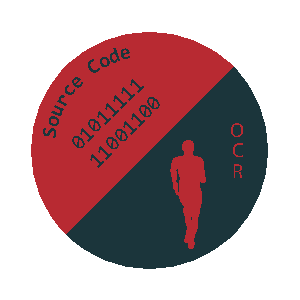
\includegraphics[width=0.4\linewidth]{images/logo}
	\caption{Chicken chien}\label{fig:Chicken1}%% anpassen
\end{figure}

Text (\autoref{fig:Chicken2} und \autoref{fig:Chicken1}).

\begin{figure}[!hb]% hier: !hb
	\centering
	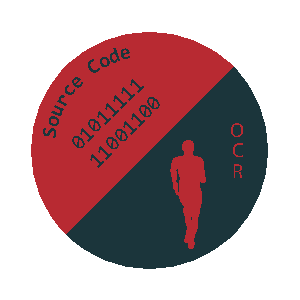
\includegraphics[height=0.4\linewidth,angle=90]{images/logo}
	\caption{Bild 90 Grad drehen.}\label{fig:Chicken2}%% anpassen
\end{figure}


\section{Quelltext}
\verb|\lstinline| oder \verb|\verb|.

\paragraph{verb}
Bsp. \verb|int|, \verb|bool| (\autoref{code:one}).

\paragraph{lstlisting}

\lstset{language=C++}% C, TeX, Bash, Python
\begin{lstlisting}[%% anpassen
caption={Es ist eine alte Tradition, eine neue Programmiersprache mit einem Hello-World-Programm einzuweihen. Auch dieses Buch soll mit der Tradition nicht brechen, hier ist das Hello-World-Programm in C++}, label=code:one]
// Ein- und Ausgabebibliothek
#include <iostream>

int main(){// Hauptfunktion
	std::cout << "Hallo Welt!" << std::endl;// Ausgabe
	return 0;
}
\end{lstlisting}

\section{Tabellen neu}

(\autoref{tab:tabneu}).
\begin{table}[!ht]% hier: !ht
	\centering 
	\caption{Tabelle neu, gute Beschreibung einfügen}\label{tab:tabneu}%% anpassen
	\begin{tabular}{@{}rlc@{}}
	\toprule 
    \textbf{Nr.} & \textbf{Begriffe} & \textbf{Erklärung}\\
	\midrule
    1 & a1 & a2\\
    2 & b1 & b2\\
    3 & c1 & c2\\
    4 & a1 & a2\\
	\bottomrule
 	\end{tabular}
\end{table}


\section{Gleichungen}

$x$--$y$, \( x^2 + y^2 = 1 \)

(\autoref{eq:summe}).
\begin{equation}\label{eq:summe}%% anpassen
	\sum \limits_{i=1}^n i = \frac{n(n+1)}{2}
\end{equation}




%\chapter{vorlage-abbildungen}
%\textbf{Vorlage -- Abbildungen}

Abbildung1 (\autoref{fig:Abbildung1}).
%
\begin{figure}[!hb]% hier: !hb
	\centering
	\includegraphics[width=.60\textwidth]{images/Chili-1.pdf}%
	\caption{Abbildung1}\label{fig:Abbildung1}%% anpassen
\end{figure}

Abbildung2 (\autoref{fig:Abbildung2}).
%
\begin{figure}[!hb]% hier: !hb
	\centering
	\includegraphics[width=.95\textwidth]{images/Logo-Details.eps}%
	\caption{Abbildung2}\label{fig:Abbildung2}%% anpassen
\end{figure}


Logo in Neg, Grau, Schwarz (\autoref{fig:logoneggrauschwarz}).
%
\begin{figure}[!hb]% hier: !hb
	\centering
	\begin{minipage}[b]{0.40\textwidth}
		
\includegraphics[width=\textwidth]{images/Logo-negativ.eps}%
	\end{minipage}
	\hfill
	\begin{minipage}[b]{0.30\textwidth}
		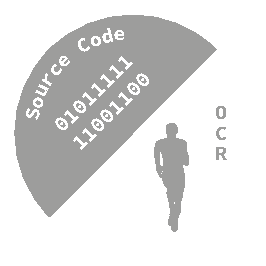
\includegraphics[width=\textwidth]{images/Logo-Grau.eps}%
	\end{minipage}
	\hfill
	\begin{minipage}[b]{0.20\textwidth}
		
\includegraphics[width=\textwidth]{images/Logo-SW.eps}%
	\end{minipage}
	\caption{Logo in Neg, Grau, Schwarz}\label{fig:logoneggrauschwarz}%% anpassen
\end{figure}



%\chapter{vorlage-literaturangabe-kfz}
%% letztes Update: 28-Jul-20
\textbf{Zitat -- KFZ}

Quelle: ~\textcite{schmidt:2015:klima}

Quelle: ~\textcite{sternbeck:2015:bremsen}

Quelle: ~\textcite{schneehage:2018:aktoren}

Quelle: ~\textcite{frei:2017:hochvolt}

Quelle: ~\textcite{frei:2013:elektrik}

Quelle: ~\textcite{gunther:2019:commonrail}

Quelle: ~\textcite{peter:2015:benzindirekt}

Quelle: ~\textcite{schneehage:2014:sensoren}

Quelle: ~\textcite{frei:2018:vernetztesysteme}

Quelle: ~\textcite{bosch:2020:training}

%\chapter{vorlage-literaturangabe-sport}
%% letztes Update: 28-Jul-20
\textbf{Zitat -- Sport}

\textbf{Kraft}

Quelle: ~\textcite{lauren:2014:fit90tage}

Quelle: ~\textcite{lauren:2016:fitkraftstoff}

Quelle: ~\textcite{lauren:2017:fit}

\textbf{Laufen}

Quelle: ~\textcite{marquardt:2015:laufbibel}

Quelle: ~\textcite{steffny:2006:laufbuch}

Quelle: ~\textcite{zeller:2017:hindernis}

\textbf{Lauftechnik verbessern}

Quelle: ~\textcite{marquardt:2018:laufstil}

\textbf{Fußtraining}

Quelle: ~\textcite{marquardt:2018:fusstraining}

Quelle: ~\textcite{marquardt:2018:fusstrainingsplan}

\textbf{Trainingsrechner}

\begin{itemize}
\item
  Tempo und die Durchgangszeiten Wettkampf
\item
  Schrittfrequenz
\item
  Zeit/Gewicht
\item
  Lauftempo in Min/km, km/h und m/s umrechnen
\item
  Wettkampfzeit
\item
  Pulsbereiche
\item
  Intervallzeiten
\item
  BMI
\item
  Kalorien/Energie
\end{itemize}

Quelle: ~\textcite{marquardt:2018:trainingsrechner}

\textbf{Trainingspuls finden}

Quelle: ~\textcite{marquardt:2018:pulspace}

\textbf{Trainingspläne für Läufer}

Quelle: ~\textcite{marquardt:2018:trainingsplan5km}

Quelle: ~\textcite{marquardt:2018:trainingsplan10km}

Quelle: ~\textcite{marquardt:2018:trainingsplan21km}

Quelle: ~\textcite{marquardt:2018:trainingsplan42km}

\textbf{Athletik}

Quelle: ~\textcite{marquardt:2018:koordinationstrainingeinsteiger}

Quelle: ~\textcite{marquardt:2018:koordinationstraininglaufen}

Quelle: ~\textcite{marquardt:2018:rueckenuebung}

Quelle: ~\textcite{marquardt:2018:knieuebung}

Quelle: ~\textcite{marquardt:2018:fussuebung}

\textbf{Sport Verletzung}

Quelle: ~\textcite{marquardt:2018:schmerzendesknie}

Quelle: ~\textcite{marquardt:2018:verletzteachilles}

\textbf{Sport Check-up}

Quelle: ~\textcite{marquardt:2018:sportmedizinischertest}

Quelle: ~\textcite{marquardt:2018:bewegungsanalyse}

Quelle: ~\textcite{marquardt:2018:leistungsdiagnostik}

Quelle: ~\textcite{marquardt:2018:laufschuhberatungssysteme}

%\chapter{vorlage-literaturangabe}
%% letztes Update: 28-Jul-20
\textbf{Zitat}

Quelle: ~\textcite{monk:2014:raspberry}

Quelle: ~\textcite{monk:2016:action}

Quelle: ~\textcite{monk:2013:elektronikhacks}

Quelle: ~\textcite{weigend:2018:python}

Quelle: ~\textcite{weigend:2016:raspberry}

Quelle: ~\textcite{schlosser:2016:latex}

Quelle: ~\textcite{homofaciens:2018:projekt}

Quelle: ~\textcite{bartmann:2018:bastelseite}

Quelle: ~\textcite{bartmann:2017:arduino}

Quelle: ~\textcite{joos:2018:windows}

Quelle: ~\textcite{joos:2012:win7}

Quelle: ~\textcite{kofler:2018:infoseite}

Quelle: ~\textcite{kofler:2015:raspberry}

Quelle: ~\textcite{kofler:2017:linux}

Quelle: ~\textcite{kofler:2018:hacking}

Quelle: ~\textcite{kofler:2016:shellbefehle}

Quelle: ~\textcite{kuveler:2009:inf}

Quelle: ~\textcite{loviscach:2018:videos}

Quelle: ~\textcite{riesinger:2017:mathe}

Quelle: ~\textcite{riesinger:2006:inf}

Quelle: ~\textcite{schwichtenberg:2017:ps}

Quelle: ~\textcite{heiderich:2016:technprobleme}

Quelle: ~\textcite{will:2014:einfuehrungcpp}

Quelle: ~\textcite{will:2018:handbuchcpp}

Quelle: ~\textcite{preisel:2017:git}

Quelle: ~\textcite{theis:2017:einstiegcpp}

Quelle: ~\textcite{theis:2017:einstiegc}

Quelle: ~\textcite{theis:2017:einstiegphp}

Quelle: ~\textcite{theis:2017:einstiegpython}

Quelle: ~\textcite{gaicher:2012:programmierenc}

Quelle: ~\textcite{gaicher:2015:avrc}

Quelle: ~\textcite{plotzeneder:2013:powerprojektec}

Quelle: ~\textcite{kuhlee:2012:forensik}

Quelle: ~\textcite{erickson:2008:hacking}

Quelle: ~\textcite{ernesti:2015:python}

